\documentclass[american]{ntnuthesis}

%\geometry{showframe}

\usepackage{epigraph}

\usepackage{pgf,tikz,tikz-3dplot}
\usetikzlibrary{arrows,arrows.meta}
\usetikzlibrary{positioning}
\usetikzlibrary{math,calc}
\usepackage{pgfplots} 
\pgfplotsset{compat=newest}

\usepackage{import}

\usepackage{amsthm}
\usepackage{mathtools}
\usepackage{bm}
\usepackage{multirow,multicol,tabularx}

\usepackage{siunitx}
\usepackage{xfrac}

\captionsetup[sub]{font=footnotesize}

\usepackage{xcolor}
\definecolor{emerald}{RGB}{0,128,0}
\definecolor{navy}{RGB}{0,0,128}
\definecolor{maroon}{RGB}{128,0,0}

\newtheorem{asm}{Assumption}
\newtheorem{prop}{Proposition}
\newtheorem*{rmk}{Remark}
\newtheorem{lemma}{Lemma}
\newtheorem{theorem}{Theorem}
\newtheorem{innercustomasm}{Assumption} % assumption with custom number
\newenvironment{customasm}[1]
  {\renewcommand\theinnercustomasm{#1}\innercustomasm}
  {\endinnercustomasm}
\newtheorem{dfn}{Definition}

\newcommand{\figref}[1]{Figure~\ref{#1}} % unify references to figures

\newcommand*{\scale}[2][1]{\scalebox{#1}{\ensuremath{#2}}}
\newcommand{\mat}[1]{\mathbf{#1}} % vectors/matrices
\newcommand{\bs}[1]{\bm{#1}}      % bold Greek symbols
\newcommand{\T}{^{\mathrm{T}}}
\newcommand{\inlinevector}[1]{\left[#1\right]\T}
\newcommand{\norm}[1]{\left\|#1\right\|}
\newcommand{\abs}[1]{\left|#1\right|}

\newcommand{\pose}{\bs{\eta}}
\newcommand{\vel}{\bs{\nu}}
\newcommand{\ocean}{\mat{V}_c}
\newcommand{\oceanhat}{\hat{\mat{V}}_c}
\newcommand{\oceantilde}{\tilde{\mat{V}}_c}
\newcommand{\mass}{\mat{M}}
\newcommand{\cor}{\mat{C}\left(\bs{\nu}_r\right)}
\newcommand{\drag}{\mat{D}\left(\bs{\nu}_r\right)}
\newcommand{\grav}{\mat{g}\left(\pose\right)}
\newcommand{\rot}{\mat{R}\left(\theta, \psi\right)}
\newcommand{\trans}{\mat{T}\left(\theta\right)}
\newcommand{\transform}{\mat{J}\left(\pose\right)}

\DeclareMathOperator*{\argmin}{arg\,min}
\DeclareMathOperator*{\diag}{diag}
\DeclareMathOperator*{\blkdiag}{blkdiag}
\DeclareMathOperator*{\rank}{rank}

\title{Cooperative Control of Formations of Underwater Vehicles}
\shorttitle{Cooperative Control of Formations of Underwater Vehicles}
\author{Josef Matou\v{s}}
\shortauthor{J. Matou\v{s}}
\setyear{2023}
\setmonth{May}
\isbnprinted{}
\isbnelectronic{}
\serialnumber{}

\addbibresource{references-introduction.bib}
\addbibresource{references-ccta.bib}
\addbibresource{references-5dof_nsb.bib}
\addbibresource{references-nsb_R.bib}
\addbibresource{references-distr_NSB.bib}
\addbibresource{references-background.bib}


% From https://www.overleaf.com/learn/latex/Glossaries

\makeglossaries % Prepare for adding glossary entries

% --------------------
% ----- Acronyms -----
% --------------------

\newacronym{phd}{PhD}{Philosophiae Doctor}
\newacronym{ntnu}{NTNU}{Norwegian University of Science and Technology}
\newacronym{itk}{ITK}{Department of Engineering Cybernetics}
\newacronym{auf}{AUF}{Autonomous Underwater Fleets}
\newacronym{auv}{AUV}{autonomous underwater vehicle}
\newacronym[longplural={degrees of freedom}]{dof}{DOF}{degree of freedom}
\newacronym{colav}{COLAV}{collision avoidance}
\newacronym{mpc}{MPC}{model predictive control}
\newacronym{cbf}{CBF}{control barrier function}
\newacronym{asv}{ASV}{autonomous surface vehicle}
\newacronym{ned}{NED}{north-east-down}
\newacronym{los}{LOS}{line-of-sight}
\newacronym{dune}{DUNE}{Unified Navigation Environment}
 % add glossary and acronym lists before document

\begin{document}

\chapter*{Summary}

This thesis investigates various control algorithms for marine vehicles.
Most of the algorithms proposed in the thesis address the formation path-following problem for a fleet of underactuated \acrlongpl{auv}, although other types of vehicles, such as \acrlongpl{asv} and differential drive robots, and other types of control problems, such as collision avoidance, trajectory tracking, and path following, are also considered.
The thesis is divided into three parts.

In the first part, we develop a collision avoidance algorithm for overactuated vehicles.
The vehicles must reach a desired position while maintaining some minimum safety distance from each other.
To solve this problem, we propose an optimization-based control allocation scheme augmented with \acrlongpl{cbf}.
Control allocation is a collection of methods for finding an actuator configuration that satisfies a given goal (\emph{e.g.}, reaching a desired position),
while \acrlongpl{cbf} allow us to enforce constraints on dynamical systems (\emph{e.g.}, keeping a minimum safety distance).
By combining control allocation with \acrlongpl{cbf}, we can create a controller that satisfies a given goal while avoiding collisions.
The proposed controller is tested in numerical simulations on two types of \acrlongpl{asv}: the milliAmpere ferry, and the Inocean Cat I drillship.

The second part addresses the formation path-following problem.
We propose to solve the problem using the \acrlong{nsb} method.
This method allows us to decompose the problem into several tasks.
Then, by combining these tasks in a hierarchic manner, we can achieve the desired behavior.
To solve the formation path-following problem, we define three tasks: collision avoidance, formation keeping, and path following.
In this thesis, we develop and analyze three different \acrlong{nsb} algorithms for the formation path-following problem.
The first algorithm uses a model of an \acrlong{auv} with five \acrlongpl{dof}.
Using Lyapunov analysis, we show that the path-following task is \acrlongpl{usges}.
Numerical simulations then validate this result.
The second algorithm uses a six-degree-of-freedom model.
Compared to the previous method, this algorithm does not suffer from numerical singularities.
This algorithm also contains additional tasks, namely obstacle avoidance and depth limiting.
Moreover, we prove that both the path-following and the formation-keeping tasks are \acrlongpl{usges}.
These theoretical results are then validated in numerical simulations.
One issue with \acrlong{nsb} algorithms is that they are centralized.
In many applications, centralized algorithms are difficult to implement, as they require a central node or an agent that can communicate and coordinate with other agents in real-time.
To solve this issue, the third algorithm combines the \acrlong{nsb} method with consensus, resulting in a fully distributed controller.
We propose two types of consensus algorithms.
First, we propose a continuous-time consensus algorithm and prove its stability using Lyapunov analysis.
Then, we present a modified discrete-time version of the algorithm based on event-triggered control.
The effectiveness of both the continuous- and discrete-time algorithms is demonstrated in numerical simulations.
Furthermore, the discrete-time version is also tested in field experiments.

The third part of the thesis extends the hand position approach to underactuated underwater vehicles moving in three dimensions.
This approach was originally developed to stabilize nonholonomic vehicles.
By treating the hand position of the vehicle as the output of the system, we can use input-output feedback linearization to transform the underactuated highly nonlinear vehicle model into a system with linear external dynamics and nonlinear internal dynamics.
We analyze the closed-loop behavior of a generic hand position-based controller and present four applications of the hand position approach.
First, we use this approach to solve the trajectory-tracking and path-following problems.
We propose simple PID-based controllers to solve these problems and show that using these controllers renders the external states \acrlongpl{ges}, while the internal states remain bounded.
The theoretical results are validated in numerical simulations as well as field experiments.
Next, we present a spline-based \acrlong{mpc} method for solving the formation path-following problem.
The proposed method is not restricted to the hand position approach only.
In fact, the method is applicable to any vehicle with a differentially flat model.
To demonstrate this, we present two case studies: underwater vehicles with the hand position controller, and differential drive robots.
Next, we use the hand position concept to solve the tracking-in-formation problem for a fleet of \acrlongpl{auv}.
The proposed method combines consensus with \acrlongpl{blf}, allowing the fleet to reach the desired formation while avoiding collisions and maintaining connectivity.
We show that the closed-loop system is almost-everywhere uniformly asymptotically stable and that the output error dynamics converge to the origin exponentially fast while satisfying the constraints.
The theoretical results are verified in numerical simulations.
Finally, we combine the hand position approach with \acrlong{nsb} control.
Specifically, we extend the \acrlong{nsb} algorithm, which was originally developed for first-order kinematic systems, to second-order systems.
Similarly to our previous work, we then design the path-following, formation-keeping, and collision-avoidance tasks, so that the fleet can follow a given path in a formation while avoiding collisions.
We prove the stability of the control scheme using Lyapunov analysis and verify its effectiveness in simulations. 

\chapter*{Preface}

This thesis is submitted in partial fulfillment of the requirements for the degree of \gls{phd} at the \gls{ntnu}, Trondheim.

The work presented has been conducted at the \gls{itk}, \gls{ntnu}, as part of the \gls{auf} project.
Professor Kristin Ytterstad Pettersen from the \gls{itk} has been the main supervisor. 
Professor Damiano Varagnolo from the \gls{itk} and Department of Information Engineering, University of Padova, Italy, and doctor Claudio Paliotta from SINTEF Digital and Aker Solutions have been the co-supervisors.
This work was partly supported by the Research Council of Norway through project No. 302435 and the Centres of Excellence funding scheme, project No. 223254.

\section*{Acknowledgments}

First and foremost, I would like to thank my supervisor, Kristin.
Not only she gave me this opportunity to study PhD, but she has also been an excellent supervisor, always positive and optimistic, gently nudging me towards the right direction. 
Furthermore, she possesses an incredible ability to refine my very coarse ideas into something presentable.

I would also like to thank my co-supervisors, Damiano and Claudio, for taking the time off their very busy schedules to guide and help me.
I remember that on multiple occasions, Damiano took a half-day off just to give me detailed feedback on my work, and Claudio has continued to work with me even after leaving SINTEF and getting a new job at Aker Solutions.
Thank you both for that.

I also must not forget to thank my former supervisors from the Czech Technical University in Prague, Tomáš Michálek and Martin Gurtner, as well as the head of the research group, Professor Zdeňek Hurák, for helping me to find the position at NTNU and encouraging me to apply.

The work presented in this thesis is not a work of a single person.
To this end, I would like to thank everyone who contributed to the presented results.
This includes my supervisors, as well as Erlend Basso and Emil Thyri, who helped me with my very first scientific paper, Esteban Restrepo, who visited NTNU for two months in 2022 and with whom we have had a fruitful collaboration ever since, and Erling Lie, whose brilliant Master's project became a conference paper.

Demonstrating that the presented theory actually works typically requires some nice plots and results.
While numerical simulations are nice, there is no substitute for field experiments with very expensive and delicate hardware placed in a hostile environment.
To this end, I would like to thank Professor Jo\~{a}o Tasso de Figueiredo Borges de Sousa and the engineering team at Laborat\'{o}rio de Sistemas e Tecnologias Subaqu\'{a}ticas (LSTS), Faculty of Engineering, University of Porto, and Prof. Martin Ludvigsen, Dr. Antonio Vasilijevic, and the engineering team at the Applied Underwater Robotics Laboratory (AUR-lab), NTNU, for providing access to their underwater vehicles and facilities, and invaluable support before and during the experiments. 
In addition, I wish to thank Tore Mo-Bjørkelund from the AUR-lab and Renato Campos from OceanScan-MST for their help with deploying the control algorithms to the vehicles.

Furthermore, I would like to thank all my friends and colleagues at NTNU for helping me to survive these incredible three years.
Last but not least, I would like to thank my family, my father Josef, my mother Vladislava, and my sister Vladim\'{i}ra, for their support and the relaxing summer and Christmas holidays.


\tableofcontents
%\listoffigures
%\listoftables
%\lstlistoflistings

\printglossary[type=\acronymtype] % Print acronyms
%\printglossary                    % Print glossary
%\printunsrtglossary[type=symbols,style=long]
\chapter*{List of Symbols}

\begin{tabularx}{\textwidth}{lX}
    \ensuremath{\mathbb{R}}              & The set of real numbers. \\
    \ensuremath{\mathbb{Z}_{\geq 0}}     & The set of nonnegative integers. \\
    \ensuremath{\mathbb{R}^n}            & The set of $n$-dimensional real vectors. \\
    \ensuremath{\mathbb{R}^{n \times m}} & The set of $n$-by-$m$ real matrices. \\
    \ensuremath{SO(3)}                   & The special orthogonal group of dimension 3. \\
    \ensuremath{\mathfrak{so}(3)}        & The space of 3-by-3 skew-symmetric matrices, and the Lie algebra of $SO(3)$. \\
    \ball[n]{r}                          & The $n$-dimensional ball of radius $r$ ($\ball[n]{r} = \left\{\mat{x} \in \mathbb{R}^n | \norm{\mat{x}} \leq r\right\}$). \\
    \ensuremath{\mat{I}_n}               & The $n$-by-$n$ identity matrix. \\
    \ensuremath{\mat{O}_{n \times m}}    & The $n$-by-$m$ null matrix. \\
    \ensuremath{\mat{0}_{n}}             & The $n$-dimensional null vector. \\
    \ensuremath{\mat{1}_{n}}             & The $n$-dimensional vector of ones. \\
    \ensuremath{\mat{1}_{n \times m}}    & The $n$-by-$m$ matrix of ones. \\
    \ensuremath{\norm{\mat{x}}}          & The Euclidean norm of a vector $\mat{x} \in \mathbb{R}^n$. \\
    \ensuremath{\mat{A}^{\dagger}}       & The Moore-Penrose pseudoinverse of a matrix $\mat{A} \in \mathbb{R}^{n \times m}$. \\
    \ensuremath{\mat{A} \otimes \mat{B}} & The Kronecker tensor product of matrices $\mat{A} \in \mathbb{R}^{n_a \times m_a}$ and $\mat{B} \in \mathbb{R}^{n_b \times m_b}$. \\
    \ensuremath{\arctan_2}               & Four-quadrant inverse tan; $\arctan_2(y, x)$ is equivalent to the phase of the complex number $x + iy$.
\end{tabularx}


\chapter{Introduction}
\label{chap:introduction}

\setlength{\epigraphwidth}{0.5\textwidth}
\epigraph{ \it
    In the beginning the Universe was created.
    This has made a lot of people very angry and been widely regarded as a bad move.
}{--- Douglas Adams, ``The Restaurant at the End of the Universe,'' 1980.}

\section{Motivation}

\section{Literature Review and Motivation}
\label{sec:introduction_literature}

In this section, we present a general introduction to the problems studied in the thesis, as well as an overview of the existing literature.

\subsection{Marine Robots}

In this section, we briefly introduce the three main types of marine robots and their use.
Unmanned marine vehicles are being increasingly used in a variety of applications such as transportation \cite{pi_transportation_2021,brekke_milliampere_2022}, inspection, maintenance and repair \cite{palomer_inspection_2019,mcleod_inspection_repair_maintenance_2010}, mapping of underwater structures, \emph{e.g.,} shipwrecks \cite{bingham_shipwreck_2010}, and various oceanographic and environmental missions such as tracking of oil spills \cite{petillo_plume_tracking_2012} and harmful algal blooms \cite{robbins_harmful_algae_2006}.
These vehicles often operate in environments that are inaccessible or dangerous to humans, such as the deep sea or the Arctic.

Marine robots can generally be split into three categories: \glspl{asv}, \glspl{rov}, and \glspl{auv}.
\Glspl{asv} are also referred to as \emph{autonomous ships}, since their design is commonly based on surface vessels such as kayaks \cite{kimball_jetkayak_2014}, catamarans \cite{choi_asv_2020,zolich_catamaran_2022}, and miniature ferries \cite{brekke_milliampere_2022}. \Glspl{asv} are used in scientific missions as well as transportation.
\Glspl{rov}, also referred to as \emph{underwater drones}, are small, box-shaped vehicles with thrusters.
\Glspl{rov} are typically \emph{fully actuated}, meaning that the configuration of thrusters allows the vehicle to move and rotate in any direction.
\Glspl{rov} are designed for low speeds, often less than $1.5$ meters per second, and due to the high power demands of the thrusters, the vehicles can only operate for a few hours \cite{bluerov2}.
Consequently, \glspl{rov} are used for short-term inspection, maintenance and repair missions.
To complete these missions, \glspl{rov} are connected to an operator via a series of cables, referred to as the \emph{tether}.

Conversely, \glspl{auv} are able to operate independently and without any connecting cables.
There are various types of \glspl{auv}.
This thesis studies slender, torpedo-shaped \glspl{auv} with a propeller that provides forward (surge) thrust, and fins that provide torque.
This configuration of actuators means that these \glspl{auv} are \emph{underactuated}, as we cannot directly control the lateral (sway and heave) velocities.
Compared to \glspl{rov}, \glspl{auv} can reach higher speeds and operate longer \cite{sousa_LAUV_2012,purcell_remus_2000}, making them suitable for long-term oceanographic missions.
%This thesis is mostly focused on developing control algorithms for \glspl{auv}.

\subsection{Control Problems for AUVs}

This section presents the various control problems for \glspl{auv} studied in this thesis.

\subsubsection{The Trajectory-Tracking and Path-Following Problems}

Arguably, the trajectory-tracking and path-following problems are the most interesting and significant ones,
since many high-level mission planners assume that the vehicle is able to follow a given path or trajectory.

\dt{
For the purposes of this thesis, a path is a curve (\emph{i.e.,} a one-dimensional object in two- or three-dimensional Euclidean space), while a trajectory is a time-varying reference position.
In the literature, it is often stated that a trajectory is a ``path with temporal constraints'' \cite{paliotta_trajectory_2019}.
Consequently, in trajectory tracking, the desired position of the vehicle for a given time is fixed, while in path following, we have some freedom in choosing which point on the desired path should be followed at a given time.
A more detailed discussion on the differences between trajectory tracking and path following is presented in Section~\ref{sec:background_formation_path_following}.
}

To solve the trajectory-tracking problem, numerous methods based on backstepping \cite{rezazadegan_trajectory-tracking-backstepping_2015,alonge_trajectory-tracking-backstepping_2001}, sliding-mode control \cite{elmokadem_trajectory-tracking-SMC_2016}, \glspl{clf} \cite{aguiar_trajectory-tracking-CLF_2007}, and \gls{mpc} \cite{abdelaal_trajectory-tracking-MPC_2015} have been proposed. 

To solve the path-following problem, most controllers utilize \gls{los} guidance.
In \cite{caharija_path-following-ILOS_2016}, an integral \gls{los} guidance scheme is used to counteract the sea loads, \cite{xiang_path-following-robust_2017} combines \gls{los} guidance with an adaptively tuned PID controller, and \cite{miao_path-following-curvilinear_2017} uses \gls{los} with active disturbance rejection control.

\subsubsection{The Formation Path-Following Problem}

%\Glspl{auv} are being increasingly used in a number of applications such as transportation \cite{conti_manipulation_2015}, oceanography \cite{edgar_oceanography_2001,faria_oceanography_2014}, and ocean energy industry-related tasks \cite{albiez_flatfish_2015,lizunkova_AUVwelding_2009}.
In many applications, it is advantageous to perform the tasks with a group of cooperating \glspl{auv}.
Compared to a single vehicle, a group of \glspl{auv} can cover a larger area (\emph{e.g.,} in inspection and oceanographic tasks).
A group is also more flexible, able to reconfigure if the parameters of the mission change, and able to complete the task even if one or more \glspl{auv} fail.
Many of the aforementioned applications can be formulated as a formation path-following problem, \emph{i.e.,} a problem of steering a group of \glspl{auv} along a predefined path in a given formation.

As presented in \cite{das_cooperative_2016}, there exists a plethora of formation path-following methods, most of them based on two concepts: coordinated path-following \cite{borhaug_2006_formation,praveen_cooperative_2018} and leader-follower \cite{rongxin_2010_leader,soorki_2011_robust}.
In the \emph{coordinated path-following} approach, each vehicle follows a predefined path separately.
Formation is then achieved by coordinating the motion of the vehicles along these paths.
In this approach, the formation-keeping error (\emph{i.e.,} the difference between the actual and desired relative position of the vehicles) may initially grow as the vehicles converge to their predefined paths.
In the \emph{leader-follower} approach, one leading vehicle tracks the given path while the followers adjust their speed and position to obtain the desired formation shape, relative to the leader.

Both the coordinated path-following and the leader-follower method can be solved using \acrlong{mpc} \cite{wang_path_2021,kanjanawanishkul_distributed_2008}.
\Gls{mpc} is a model-based optimal control method that allows us to enforce constraints on the inputs and states of the vehicles.
However, most \gls{mpc} methods are based on sampling.
Consequently, any constraints on the inputs or states can only be enforced at discrete-time instances.
In other words, we have no control over the behavior of the system between the samples.
We can mitigate this issue by decreasing the sampling time.
However, by decreasing the sampling time, we increase the number of optimized variables, thus increasing the computational requirements.

In recent years, researchers have focused on computationally tractable \gls{mpc} schemes.
One possibility of reducing the computational requirements is to parametrize the vehicles' trajectories using splines.
A spline-based path-planning \gls{mpc} algorithm for first-order nonholonomic vehicles was proposed \cite{saska_2016_predictive}.
The algorithm solves the point-to-point formation tracking problem with static obstacles.
Another spline-based \gls{mpc} algorithm was proposed in \cite{van_parys_2017_DMPC}.
This algorithm is applicable to a wider range of systems compared to \cite{saska_2016_predictive}, and it has been demonstrated on point-to-point and trajectory-tracking problems.

Another method that can be applied to the formation path-following problem is the so-called \gls{nsb} algorithm \cite{antonelli_experiments_2009,arrichiello_formation_2006,pang_2019_formation,eek_formation_2021}.
In the \gls{nsb} framework, the control objective is expressed using multiple tasks.
By combining several simple tasks, the vehicles can exhibit the desired complex behavior.
In the literature, there are many examples of \gls{nsb} algorithms applied to kinematic vehicles \cite{antonelli_experiments_2009} and marine vehicles moving in the 
horizontal plane \cite{arrichiello_formation_2006,pang_2019_formation,eek_formation_2021}.

However, the standard \gls{nsb} algorithm is centralized, meaning that in a real-life application, there must be a central node that communicates and coordinates with all the vehicles.
While underwater, the \glspl{auv} typically communicate via acoustic modems.
These modems have low bandwidth and significant delays, making them unsuitable for real-time control.
A distributed \gls{nsb} algorithm was proposed in \cite{ahmad_multirobot_2014}.
In this algorithm, the group of vehicles is split into smaller, fully connected subgroups.
Each subgroup performs the standard, centralized \gls{nsb} algorithm.
%Consequently, there is still a need for fast and reliable communications.
The proposed method is limited to static formations.
A similar scheme was proposed in \cite{tan_coordinated_2022}, where a group of heterogenous surface vehicles is split into homogenous subgroups.
Each subgroup has one leading vehicle that exchanges information with the leaders of other subgroups.
%This scheme still requires fast and reliable communications, both within the subgroups and between the leaders.
%Furthermore, the proposed scheme is vulnerable to failures of the leading vehicles.

\subsection{Safety Constraints}
\label{sec:introduction_safety}

This section presents the various constraints that need to be considered when deploying autonomous vehicles.

\subsubsection{Collision Avoidance}
Autonomous vehicles are often used in cluttered and unpredictable environments where considerations to other vehicles and obstacles need to be made. 
Therefore, the control system of autonomous vehicles should include some form of \gls{colav}.

Reviews of various \gls{colav} concepts are presented in \cite{statheros_autonomous_2008,tam_review_2009,hoy_algorithms_2015}.
In general, algorithms for \gls{colav} can be split into two categories: motion planning and reactive algorithms.

Motion planning algorithms include, among others, various types of path planning algorithms \cite{wang_ship_2017,kuwata_safe_2014,chiang_colreg-rrt_2018,lazarowska_ships_2015}, the dynamic window algorithm \cite{fox_dynamic_1997}, and \gls{mpc}.
\gls{mpc} can be used both for a single vehicle \cite{hagen_mpc-based_2018,sun_collision_2018} and for multi-agent systems in a distributed form \cite{kuriki_formation_2015,dai_distributed_2017}.
Some motion planning algorithms also include consideration of relevant traffic protocols that apply in the given domain, \emph{e.g.,} the regulations for marine vehicles known as COLREGs \cite{wang_ship_2017,kuwata_safe_2014,chiang_colreg-rrt_2018}.

Reactive algorithms for \gls{colav} include, among others, virtual potential fields \cite{roussos_3d_2008}, geometric guidance \cite{mujumdar_reactive_2011}, and \glspl{cbf} \cite{squires_constructive_2018,igarashi_collision_2018,romdlony_stabilization_2016,basso_safety-critical_2020,ames_control_2014}.
Reactive algorithms are often used together with motion planning algorithms in a hybrid controller.
In such a controller, the reactive algorithm ensures the safety of the vehicle in unexpected situations.
Such an algorithm is proposed in \cite{hedjar_automatic_2019}, where a collision-free velocity reference is obtained through numerical optimization.
%The proposed algorithm is designed specifically for \glspl{asv}.

\Glspl{cbf} offer a \gls{colav} method that is applicable to a wide range of systems \cite{ames_control_2019}.
In the literature, there are typically two ways in which \glspl{cbf} are applied for \gls{colav}.
They are either applied to a simplified model of the vehicle (\emph{e.g.,} a unicycle model \cite{squires_constructive_2018,igarashi_collision_2018}) to provide safe velocity references, or they are used together with \glspl{clf} \cite{romdlony_stabilization_2016,basso_safety-critical_2020,ames_control_2014} on the complete model.

Reactive \gls{colav} methods that work with a simplified model do not take into account the physical limitations of the vehicle, such as acceleration or actuator constraints.
Consequently, these methods may output reference signals that the underlying controllers cannot track.
To mitigate this, reactive \gls{colav} methods should be included at the lowest-possible control level.

\subsubsection{Connectivity Maintenance}
In addition to \gls{colav}, autonomous vehicles often need to maintain a sufficiently close distance to each other to guarantee the reliability of the communication and the connectivity of the multi-agent system.
In special cases when the vehicles use optical sensors or communications, the vehicles are also limited by \gls{fov} constraints.

Many works in the literature address the coordination problem of multiple marine vehicles under such inter-agent constraints. In \cite{gan2014online,gomes2018MPC} planning-based methods are developed to generate trajectories that satisfy the constraints. However, planning algorithms usually require \emph{a priori} knowledge of the environment, which might be unrealistic in highly dynamical environments, such as under water. Reactive algorithms are based, \emph{e.g.}, on artificial potential fields \cite{jia2007formation,brinon2010contraction} and \glspl{blf} \cite{gao2019velocity-free,naderolasli2023platoon}.


\section{Research Questions}

\section{Outline}

\subsection{Unifying Reactive Collision Avoidance and Control Allocation}
\fullcite{matous_unifying_2021}.

\subsection{Formation Path-following using the Null-space-based Behavioral Algorithm}
\fullcite{matouvs_formation_2022}.

\noindent\fullcite{matous_singularity_2023}.

\noindent\fullcite{matous_distributed_2023}.

\subsection{Hand Position and Its Applications}
\fullcite{matous_trajectory_2023}.

\noindent\fullcite{matous_MPC_2022}

\noindent\fullcite{restrepo_formation_2022}

\noindent\fullcite{restrepo_tracking_2023}

\noindent\fullcite{lie_formation_2023}

\chapter{Background}
\label{chap:background}

Information on background theory, methods, etc.

\section{Geometric Paths}
\label{sec:background_paths}

This section presents the definitions of paths in the context of guidance.
The theory presented in this section applies to two- and three-dimensional Euclidean spaces.
Let $n_d \in \{2,3\}$ denote the number of dimensions.

\subsubsection*{Paths and their parametrizations}
A \emph{path} is a curve in $n_d$-dimensional space.
A \emph{parametrization} of a path is a function $\mat{p}_p : \mathbb{R} \mapsto \mathbb{R}^{n_d}$ that describes the curve.
Note that there exist infinitely many parametrizations of the same path.
For example, the following two functions
\begin{align}
    \mat{p}_{p, 1}(s) &= \inlinevector{s, 0, 0}, &
    \mat{p}_{p, 1}(s) &= \inlinevector{s^3, 0, 0}, &
\end{align}
represent the same path --- a straight line going through the origin, parallel to the $x$-axis.

\subsubsection*{Continuity and regularity}
There are two types of continuity --- \emph{parametric} and \emph{geometric}.
Parametric continuity is related to a specific parametrization of a path, while geometric continuity is related to the curve itself.
Here, we will only present the definition of parametric continuity, as it will be used furhter in the thesis.
For details on geometric continuity, the reader is referred to \cite{barsky_geometric_1984}.
Parametric continuity is denoted $\mathcal{C}_n$, where $n \in \mathbb{Z}_{\geq 0}$ is the order.
A parametrization $\mat{p}_p(s)$ is $\mathcal{C}_n$ if it is $n$-times continuously differentiable.

A parametrization if \emph{regular} if 


\chapter{Unifying Reactive Collision Avoidance and Control Allocation}
\label{chap:collision_avoidance}

To enable autonomous vehicles to operate in cluttered and unpredictable environments with numerous obstacles, such vehicles need a collision avoidance system that can react to and handle sudden changes in the environment.
This chapter discusses an optimization-based reactive collision avoidance system that uses control barrier functions integrated into the control allocation.
%We demonstrate the ability of the method to track the reference waypoints while maintaining safe distances through numerical simulations where the method is applied to autonomous surface vehicles.
We demonstrate the effectiveness of this method through numerical simulations of autonomous surface vehicles. The simulated vehicles track their reference waypoints while maintaining safe distances.
The proposed method can be readily implemented on vehicles that already use an optimization-based control allocation method.
The contents of this chapter are based on \cite{matous_unifying_2021}.

%%%%%%%%%%%%%%%%%%%%%%%%%%%%%%%%%%%%%%%%%%%%%%%%%%%%%%%%%%%%%%%%%%%%%%%%%%%%%%%%
\section{Introduction}
%Overactuated vehicles, \emph{i.e.,} vehicles with more actuators than degrees of freedom (DOFs), often use control allocation in their lowest-level controller \cite{johansen_control_2013}.
In this chapter, we consider overactuated vehicles, \emph{i.e.,} vehicles with more actuators than \acrfullpl{dof}, with a control system consisting of blocks shown in Figure \ref{fig:ccta_diagram}.
The control system contains a long-term, deliberate planner, a high-level controller that outputs desired forces and torques ($\bs{\tau}_d$), and a control allocation block.
The goal of control allocation is to find actuator control inputs ($\mathbf{u}$) that generate the desired forces and torques.
Most control allocation methods are based on numerical optimization \cite{oppenheimer_control_2006,harkegard_dynamic_2004,johansen_constrained_2004} which makes them ideal for augmenting with \acrfullpl{cbf}.

\begin{figure}[t]
    \centering
    \tikzstyle{block} = [draw, fill=white, rectangle, 
    minimum height=3em, minimum width=6em]
%\tikzstyle{sum} = [draw, fill=white, circle, node distance=1cm]
%\tikzstyle{input} = [coordinate]
\tikzstyle{pinstyle} = [pin edge={to-,thin,black}]

\begin{tikzpicture}[auto, node distance=3.75cm,>=latex']
    \node [block, align=center] (planner) {Planner};
    \node [block, right of=planner, text width=2.5cm, align=center, node distance=3cm] (highlevel) {High-level \\ controller};
    \node [block, right of=highlevel, text width=2.5cm, align=center] (alloc) {Control \\ allocation};
    \node [block, right of=alloc, align=center, node distance=3.25cm] (actuators) {Actuators};
    \draw [->] (planner) -- (highlevel);
    \draw [->] (highlevel) -- node [align=center] {$\boldsymbol{\tau}_d$} (alloc);
    \draw [->] (alloc) -- node [align=center] {$\mathbf{u}$} (actuators);
    %\draw [->] (highlevel) -- (alloc);
    %\draw [->] (alloc) -- (actuators);
\end{tikzpicture}
    %\includegraphics[width=.45\textwidth]{figures/ccta/diagram.pdf}
    \vspace{-1mm}
    \caption{Control system of overactuated vehicles considered in this chapter}
    \label{fig:ccta_diagram}
\end{figure}

The main contribution of this chapter is a reactive \acrfull{colav} algorithm that is included at the lowest level in the control pipeline, \emph{i.e.} in the control allocation, to ensure the safety of the vehicle regarding collision avoidance.
Since it is included at the lowest-possible control level, it also ensures the ``baseline'' safety of any other higher level (long term/deliberate) planners of the vehicle guidance, navigation and control system.
The algorithm can easily be implemented on vehicles that apply a numerical optimization-based method to control allocation.
Moreover, the algorithm does not rely on any communication between the vehicles; the only required information is the position and velocity of other vehicles.
The chapter extends the results in \cite{thyri_reactive_2020}, which only considers \acrfullpl{asv} and simple encounters between one \gls{asv} and a vessel moving at a constant course and speed, making the method applicable to a wider range of vehicles and scenarios with multiple autonomous vehicles.

The remainder of the chapter is organized as follows.
Section \ref{sec:ccta_model} defines the notation and describes the model of the vehicle.
The proposed control allocation method and \glspl{cbf} are introduced in Sections \ref{sec:ccta_alloc} and \ref{sec:ccta_CBF}.
%Section \ref{sec:ccta_alloc} introduces control allocation and Section \ref{sec:ccta_CBF} introduces CBFs.
Section \ref{sec:ccta_optimization} describes the resulting combined \gls{colav} and control allocation optimization problem.
Section \ref{sec:ccta_simulations} presents the results of numerical simulations using models of \glspl{asv}.
Finally, Section \ref{sec:ccta_conclusion} contains some concluding remarks.

\section{Vehicle Model}
\label{sec:ccta_model}

\subsection{Notation}
\label{sec:ccta_notation}

Let $\mathbf{p}$ denote the position and $\bs{\Theta}$ the orientation (expressed using the Euler angles) of the vehicle in a \acrfull{ned} reference frame.
%The test models presented in Section~\ref{sec:ccta_simulations} have three degrees of freedom (DOFs), with the position and orientation defined as follows
%\begin{align}
%    \mathbf{p} &= \left[ x ,\, y \right]^{\rm T}, &
%    \bs{\Theta} = \psi,
%\end{align}
%where $x$ is the North coordinate, $y$ is the East coordinate, and $\psi$ is the yaw angle.
%
Let $\pose$ be the pose of the vehicle
\begin{equation}
    \pose = \left[ \mathbf{p}^{\rm T} ,\, \bs{\Theta}^{\rm T} \right]^{\rm T}.
\end{equation}

Let $\vel$ be the velocities of the vehicle in the body-fixed frame.
%For our 3DOF models
%\begin{equation}
%    \vel = \left[ u ,\, v ,\, r \right]^{\rm T},
%\end{equation}
%where $u$ and $v$ are the surge and sway velocities, respectively, and $r$ is the yaw rate.
%
The complete state of the vehicle, $\mathbf{x}$, is defined as
\begin{equation}
    \mathbf{x} = \left[ \pose^{\rm T} \,, \vel^{\rm T} \right]^{\rm T}.
\end{equation}

Let $\bs{\tau}$ be the vector of generalized forces acting on the vehicle.
%For our 3DOF models
%\begin{equation}
%    \bs{\tau} = \left[ X ,\, Y ,\, N \right]^{\rm T},
%\end{equation}
%where $X$ and $Y$ are the forces in the surge and sway direction, respectively, and $N$ is the yaw moment.
Let $K$ be the number of actuator parameters and $\mathbf{u} \in \mathbb{R}^{K}$ the vector of inputs.
Furthermore, let $b : \mathbb{R}^{K} \rightarrow \mathbb{R}^{n_{\rm DOF}}$ be a nonlinear function that maps the inputs to the generalized forces ($n_{\rm DOF}$ is the number of \glspl{dof}).

\subsection{Equations of Motion}

The time-derivative of the pose can be obtained by transforming the velocities. % to the NED frame.
In addition, we assume that the time-derivatives of the velocities are affine in the generalized forces.
We thus consider vehicles described by the following dynamical equations
\begin{equation}
    \dot{\mathbf{x}} = \begin{bmatrix} \dot{\pose} \\ \dot{\vel} \end{bmatrix} = \begin{bmatrix}
        \mathbf{J}(\bs{\Theta})\,\vel \\ f(\mathbf{x}) + g(\mathbf{x})\,\bs{\tau}
    \end{bmatrix} = \begin{bmatrix}
        \mathbf{J}(\bs{\Theta})\,\vel \\ f(\mathbf{x}) + g(\mathbf{x})\,b(\mathbf{u})
    \end{bmatrix},
    \label{eq:ccta_affine_model}
\end{equation}

\noindent where $\mathbf{J}(\bs{\Theta})$ is the transformation matrix. % from body-fixed to NED frame. 
This equation describes a large class of systems, including the matrix-vector model of marine vessels \cite{fossen_handbook_2011}
\begin{subequations}
    \begin{align}
        \dot{\pose} &= \mathbf{J}(\bs{\Theta})\,\vel, \\
        \mathbf{M}\,\dot{\vel} + \left(\mathbf{C}(\vel) + \mathbf{D}(\vel)\right)\,\vel + \mathbf{g}(\pose) &= b(\mathbf{u}),% + \bs{\tau}_w,
    \end{align}
    \label{eq:ccta_matrix_model}
    \vspace{-4mm}
\end{subequations}

\noindent This model can be converted to the form in \eqref{eq:ccta_affine_model} since the matrix $\mathbf{M}$ is invertible.

\section{Control Allocation}
\label{sec:ccta_alloc}

As stated in the Introduction, the goal of the control allocation is to find the inputs that generate the desired forces given by the high-level controller.
For details on control allocation techniques for both linear and nonlinear systems, the reader is referred to \cite{johansen_control_2013}.

In this chapter, we consider systems where the function $b$ can be nonlinear.
In the literature, nonlinear control allocation is commonly solved by linearizing the function $b$ \cite{harkegard_dynamic_2004,johansen_constrained_2004}%, \emph{i.e.,}
\begin{equation}
    b(\mathbf{u}_0 + \Delta\mathbf{u}) \approx b(\mathbf{u}_0) + \mathbf{B}(\mathbf{u}_0)\,\Delta\mathbf{u},
    \label{eq:ccta_forces_approximation}
\end{equation}
where $\mathbf{u}_0$ are the inputs around which we linearize, $\Delta\mathbf{u}$ is the increment, and
\begin{equation}
    \mathbf{B}(\mathbf{u}_0) = \frac{\partial b(\mathbf{u})}{\partial \mathbf{u}}\bigg|_{\mathbf{u}_0},
\end{equation}
is the Jacobian of $b$ evaluated at $\mathbf{u}_0$.
Let $\bs{\tau}_d$ be the desired forces.
The goal of our control allocation scheme is to find optimal inputs $\mathbf{u}^*$ that satisfy
\begin{equation}
    \mathbf{u}^* = \argmin_{\mathbf{u}\in\mathbb{R}^{K}}\,\left\| b(\mathbf{u}) - \bs{\tau}_d \right\|^2.
\end{equation}

Using the approximation \eqref{eq:ccta_forces_approximation}, we can formulate the control allocation problem as a \acrfull{qp} 
\begin{align}
    \mathbf{u}^* &= \mathbf{u}_0 + \Delta\mathbf{u}^*, \\
    \Delta\mathbf{u}^* &= \argmin_{\Delta\mathbf{u}\in\mathbb{R}^{K}}\,\left\| b(\mathbf{u}_{0}) + \mathbf{B}(\mathbf{u}_{0})\,\Delta\mathbf{u} - \bs{\tau}_{d} \right\|^2.
\end{align} 

\section{Control Barrier Functions}
\label{sec:ccta_CBF}
In this section, we will briefly present the theory behind \acrfullpl{cbf}.
For more details, the reader is referred to \cite{ames_control_2019}.
After presenting the notation for multiple vehicles, we define the \gls{cbf} for \gls{colav}.

\subsection{Introduction to CBFs}
Consider a nonlinear control-affine system
\begin{equation}
    \dot{\mathbf{x}} = \widetilde{f}(\mathbf{x}) + \widetilde{g}(\mathbf{x})\,\mathbf{u},
    \label{eq:ccta_control_affine_system}
\end{equation}
\noindent where $\mathbf{x} \in \mathbb{R}^n$.
Suppose that the system must satisfy a safety constraint
$
    h(\mat{x}) \geq 0,
$
where $h : \mathbb{R}^{n} \rightarrow \mathbb{R}$ is the so-called \emph{barrier function}.
Then, we can define the so-called \emph{safe set}, a set of all states that satisfy the safety constraint, as
\begin{equation}
    \mathcal{C} = \left\{ \mathbf{x} \,|\, h(\mathbf{x}) \geq 0 \right\}.
\end{equation}
If the initial condition of the system \eqref{eq:ccta_control_affine_system} lies in the safe set, the system trajectory will stay within $\mathcal{C}$ if the following inequality holds \cite{ames_control_2019}
\begin{equation}
    \frac{{\rm d}}{{\rm d}t}h(\mathbf{x}) = \frac{\partial h(\mathbf{x})}{\partial \mathbf{x}}\,\left(\widetilde{f}(\mathbf{x}) + \widetilde{g}(\mathbf{x})\,\mathbf{u}\right) \geq - \gamma\bigl(h(\mathbf{x})\bigr),
    \label{eq:ccta_cbf_inequality}
\end{equation}
where $\gamma$ is an extended class-$\mathcal{K}_{\infty}$ function. 
If there exists an input $\mathbf{u}$ such that \eqref{eq:ccta_cbf_inequality} is satisfied, then $h$ is a valid \gls{cbf} for the system \eqref{eq:ccta_control_affine_system}.

\subsection{CBFs for Reactive Collision Avoidance}
%First, we need to extend the notation from Section~\ref{sec:ccta_notation} to multi-vehicle systems.
Let there be $N$ vehicles.
We shall denote the variables that belong to a given vehicle by a lower index (\emph{e.g.,} $\mathbf{x}_{i}$ is the state of the $i^{\rm th}$ vehicle).
In addition, let us define a relative position of vehicles $i$ and $j$ as
\begin{equation}
    \mathbf{p}_{ij} = \mathbf{p}_{i} - \mathbf{p}_{j}.
    \label{eq:ccta_p_ij}
\end{equation}

To ensure safety, we need a collection of \glspl{cbf} that enforce safe distances between each pair of vehicles.
In the literature, vehicles described by the model \eqref{eq:ccta_affine_model} frequently use \glspl{cbf} in the following form \cite{basso_safety-critical_2020,thyri_reactive_2020}
\begin{equation}
    %h_{ij}(\mathbf{x}_{i}, \mathbf{x}_{j}) = \|\mathbf{p}_{ij}\| - d_{\min} + k_v\,\frac{1}{\|\mathbf{p}_{ij}\|}\,\mathbf{p}_{ij}_{\rm T}\,\dot{\mathbf{p}}_{ij},
    h_{ij}(\mathbf{x}_{i}, \mathbf{x}_{j}) = \|\mathbf{p}_{ij}\| - d_{\min} + k_v\,\frac{\rm d}{{\rm d}t}\|\mathbf{p}_{ij}\|,
    \label{eq:ccta_CBF}
\end{equation}
where $d_{\min}$ is a minimum safe distance, and $k_v$ is a coefficient that penalizes the relative speed of the vehicles.

To use $h_{ij}$ as a control barrier function, we need to calculate its time-derivative.
Differentiating \eqref{eq:ccta_CBF} with respect to time yields
\begin{equation}
    \frac{\rm d}{{\rm d}t}h_{ij}(\mathbf{x}_{i}, \mathbf{x}_{j}) = \frac{\rm d}{{\rm d}t}\|\mathbf{p}_{ij}\| + k_v\,\frac{\rm d_2}{{\rm d}t_2}\|\mathbf{p}_{ij}\|.
\end{equation}

%Note that the norm $\|\mathbf{p}_{ij}\|$ can be defined as
%\begin{equation}
%    \|\mathbf{p}_{ij}\| = \sqrt{(\mathbf{p}_{ij})_{\rm T}\,\mathbf{p}_{ij}}.
%\end{equation}

%By applying the chain rule, we get
%\begin{align}
%    \frac{\rm d}{{\rm d}t}\|\mathbf{p}_{ij}\| &= \frac{1}{\|\mathbf{p}_{ij}\|}\,(\mathbf{p}_{ij})_{\rm T}\,\dot{\mathbf{p}}_{ij}, \\
%    \begin{split}
%        \frac{\rm d_2}{{\rm d}t_2}\|\mathbf{p}_{ij}\| &=  - \frac{1}{\|\mathbf{p}_{ij}\|_3}\,\left((\mathbf{p}_{ij})_{\rm T}\,\dot{\mathbf{p}}_{ij}\right)_2 \\
%        +&\frac{1}{\|\mathbf{p}_{ij}\|}\,\left((\dot{\mathbf{p}}_{ij})_{\rm T}\,\dot{\mathbf{p}}_{ij} + (\mathbf{p}_{ij})_{\rm T}\,\ddot{\mathbf{p}}_{ij}\right).
%    \end{split}        
%\end{align}

To calculate the first and second time-derivative of the relative distance, we need to find the first and second time-derivatives of the relative position.
For $\dot{\mathbf{p}}_{ij}$, we split the derivative of $\pose$ from \eqref{eq:ccta_affine_model} into the derivatives of position and orientation \vspace{-2mm}
\begin{equation}
    \dot{\pose}_{i} = \begin{bmatrix} \dot{\mathbf{p}}_{i} \\ \dot{\bs{\Theta}}_{i} \end{bmatrix} = \begin{bmatrix}
        \mathbf{J}_{\mathbf{p}}(\bs{\Theta}_{i}) \\ \mathbf{J}_{\bs{\Theta}}(\bs{\Theta}_{i})
    \end{bmatrix}\,\vel_{i}.
\end{equation}

\noindent Substituting this into the time-derivative of \eqref{eq:ccta_p_ij} yields
\begin{equation}
    \dot{\mathbf{p}}_{ij} = \mathbf{J}_{\mathbf{p}}(\bs{\Theta}_{i}) \, \vel_{i} - \mathbf{J}_{\mathbf{p}}(\bs{\Theta}_{j}) \, \vel_{j}.
    \label{eq:ccta_p_dot}
\end{equation}

\noindent For $\ddot{\mathbf{p}}_{ij}$, we assume that the target maintains its velocity, \emph{i.e.,}
\begin{equation}
    \ddot{\mathbf{p}}_{ij} \approx \ddot{\mathbf{p}}_{i},
\end{equation}
when calculating the time-derivative for the $i^{\rm th}$ vehicle.
As discussed in \cite{thyri_reactive_2020}, this is a ``mild worst-case'' assumption, since maneuvers of the target vehicle tend to aid to resolving the situation.
Thus, taking the time-derivative of \eqref{eq:ccta_p_dot} yields
\begin{equation}
    \ddot{\mathbf{p}}_{i} = \dot{\mathbf{J}}_{\mathbf{p}}(\bs{\Theta}_{i}) \, \vel_{i} + \mathbf{J}_{\mathbf{p}}(\bs{\Theta}_{i}) \, \dot{\vel}_{i}.
    \label{eq:ccta_p_ddot}
\end{equation}

Finally, we substitute the approximation of forces from \eqref{eq:ccta_forces_approximation} into the equation for $\dot{\vel}$ in \eqref{eq:ccta_affine_model} to get
\begin{equation}
    \dot{\vel}_{i} = f(\mathbf{x}_{i}) + g(\mathbf{x}_{i})\,\left(b(\mathbf{u}_{0,i}) + \mathbf{B}(\mathbf{u}_{0,i})\,\Delta\mathbf{u}_{i}\right),
\end{equation}
which we can substitute into \eqref{eq:ccta_p_ddot} to calculate $\ddot{\mathbf{p}}_{i}$.

\section{Formulating the Optimization Problem}
\label{sec:ccta_optimization}
Now we can combine the definitions from Sections~\ref{sec:ccta_alloc} and \ref{sec:ccta_CBF} to formulate the proposed optimization problem for control allocation with multi-vehicle \gls{colav}.

\subsection{The Basic Optimization Problem}
Let $\mathbf{u}_{0,i}$ be the inputs of vehicle $i$ from the previous control period.
The new inputs are calculated as
\begin{equation}
    \mathbf{u}_{i} = \mathbf{u}_{0,i} + \Delta\mathbf{u}_{i}^*,
\end{equation}
where $\Delta\mathbf{u}_{i}^*$ is obtained by solving the following \gls{qp}
\begin{subequations}
    \begin{align}
        \Delta\mathbf{u}_{i}^* &= \argmin_{\Delta\mathbf{u}_{i}\in\mathbb{R}^{K}}\,\left\| b(\mathbf{u}_{0,i}) + \mathbf{B}(\mathbf{u}_{0,i})\,\Delta\mathbf{u}_{i} - \bs{\tau}_{d,i} \right\|^2\,, \label{eq:ccta_combined_avoidance_allocation_criterion} \\
        \begin{split}
            \text{s.t. }& \frac{{\rm d}}{{\rm d}t}h_{ij}(\mathbf{x}_{i}, \mathbf{x}_{j}) \geq - \gamma\left(h_{ij}(\mathbf{x}_{i}, \mathbf{x}_{j})\right), \\
            & j \in \left\{ 1, \ldots, N \right\} \setminus \left\{ i \right\},
        \end{split} \label{eq:ccta_combined_avoidance_allocation_constraint} \\
        & \mathbf{u}_{i,\min} \leq \mathbf{u}_{0,i} + \Delta\mathbf{u}_{i} \leq \mathbf{u}_{i,\max}, \\
        & \Delta\mathbf{u}_{i,\min} \leq \Delta\mathbf{u}_{i} \leq \Delta\mathbf{u}_{i,\max}, \label{eq:ccta_combined_avoidance_allocation_delta_u}
    \end{align}
    \label{eq:ccta_combined_avoidance_allocation}
\end{subequations}
\noindent where $\mathbf{u}_{i,\min}$ and $\mathbf{u}_{i,\max}$ are the absolute actuator limits, and $\Delta\mathbf{u}_{i,\min}$ and $\Delta\mathbf{u}_{i,\max}$ are the actuator rate limits.
The absolute limits are usually given by the physical limitations of the vehicle (\emph{e.g.,} the thrust of a propeller or the deflection of control surfaces) whereas the rate limits are user-defined to reduce the rapid changes that wear out the actuators.

Simulation results using this control allocation algorithm are presented in Section~\ref{sec:ccta_simulations}.

\subsection{Modified Optimization Problem}
The algorithm in \eqref{eq:ccta_combined_avoidance_allocation} is suitable for vehicles where the number of actuators is equivalent to the number of DOFs.
Applying the algorithm to vehicles where the number of actuators is much greater than the number of DOFs results in inefficient usage of the available actuators, as can be seen in Section~\ref{sec:ccta_simulations}.

To reduce this effect, we add penalty terms on the actuator usage, similar to those proposed in \cite{johansen_constrained_2004}, in the cost function.
To simplify the notation, let $\|\mathbf{x}\|_{\mathbf{Q}}^2$ be the squared norm of a vector $\mathbf{x}$ weighted by a matrix $\mathbf{Q}$, \emph{i.e.,}
\begin{equation}
    \|\mathbf{x}\|_{\mathbf{Q}}^2 = \mathbf{x}^{\rm T}\,\mathbf{Q}\,\mathbf{x}.
\end{equation}

The modified optimization problem is defined as follows
\begin{subequations}
    \begin{align}
    \begin{split}
        \Delta\mathbf{u}_{i}^* &= \argmin_{\Delta\mathbf{u}_{i}\in\mathbb{R}^{K}}\,\left\| b(\mathbf{u}_{i,0}) + \mathbf{B}(\mathbf{u}_{i,0})\,\Delta\mathbf{u}_{i} - \bs{\tau}_{d,i} \right\|_{\mathbf{Q}}^2 \\
        &\quad \quad \quad + \left\| \mathbf{u}_{0,i} + \Delta\mathbf{u}_{i} \right\|_{\mathbf{R}_{\rm abs}}^2 + \left\|\Delta\mathbf{u}_{i}\right\|_{\mathbf{R}_{\rm rel}}^2,
    \end{split} \\    
%    \begin{split}
%        \text{s.t. }& \frac{{\rm d}}{{\rm d}t}h^{ij}(\mathbf{x}^{i}, \mathbf{x}^{j}) \geq - \gamma\left(h^{ij}(\mathbf{x}^{i}, \mathbf{x}^{j})\right), \\
%        & j \in \left\{ 1, \ldots, n \right\} \setminus \left\{ i \right\},
%    \end{split} \\
%    & \mathbf{u}^{i}_{\min} \leq \mathbf{u}^{i}_{0} + \Delta\mathbf{u}^{i} \leq \mathbf{u}^{i}_{\max}, \\
%    & \Delta\mathbf{u}^{i}_{\min} \leq \Delta\mathbf{u}^{i} \leq \Delta\mathbf{u}^{i}_{\max},
    \text{s.t. }&\text{constraints \eqref{eq:ccta_combined_avoidance_allocation_constraint}--\eqref{eq:ccta_combined_avoidance_allocation_delta_u},}
    \end{align}
    \label{eq:ccta_combined_avoidance_allocation_modified}
\end{subequations}
\noindent where $\mathbf{Q}$ is a positive definite matrix that penalizes the difference between the desired and actual forces, and $\mathbf{R}_{\rm abs}$ and $\mathbf{R}_{\rm rel}$ are positive semidefinite matrices that penalize the absolute and incremental usage of actuators, respectively.

Note that both \eqref{eq:ccta_combined_avoidance_allocation} and \eqref{eq:ccta_combined_avoidance_allocation_modified} use only local information and measurements, and can thus be solved locally for each vehicle.

When choosing the weight matrices, we first note that the vector $\bs{\tau}$ contains both forces and torques.
The matrix $\mathbf{Q}$ should penalize them differently.
In the simulations in Section~\ref{sec:ccta_simulations}, we choose
\begin{equation}
   \mathbf{Q} = \diag{(1,1,\frac{1}{L^2})},
\end{equation}
where $\diag(.)$ is a diagonal matrix and $L$ is the smallest distance of the thrusters from the center of mass.

\section{Simulations}
\label{sec:ccta_simulations}
In the simulations, we test the ability of the proposed algorithms to resolve a situation when four surface vessels are simultaneously in danger of collision.
Each vessel starts in the corner of a square and is guided towards a reference located in the diagonally opposite corner.

We tested the proposed algorithms on two models of ASVs --- the \emph{milliAmpere} ferry \cite{pedersen_optimization_2019} and the $1:90$ scaled model of the Inocean Cat I drillship \cite{bjorno_thruster-assisted_2016} --- using Simulink.
Both vessels are equipped with azimuth thrusters; the \emph{milliAmpere} has two and the drillship has six.
Each thruster is parametrized by two values: its thrust force and its azimuth.
The input vector for these vessels is defined as \vspace{-2mm}
\begin{equation}
    \mathbf{u} = \left[ f_1 ,\, \ldots ,\, f_k ,\, \alpha_1 ,\, \ldots ,\, \alpha_k \right]^{\rm T},
\end{equation}
where $f_i$ is the thrust force and $\alpha_i$ is the azimuth angle of the $i^{\rm th}$ thruster, and $k$ is the number of thrusters.
%
Both ASV models have 3DOFs, \emph{i.e.,} the North-East position and the yaw angle.
The function that maps the inputs to the generalized forces is \vspace{-2mm}
\begin{equation}
    \scale[0.93]{b(\mathbf{u}) = \sum_{i=1}^k f_i \left[ \cos\alpha_i, \sin\alpha_i, L_x^i\,\sin\alpha_i - L_y^i\,\cos\alpha_i \right]^{\rm T},}
\end{equation}
where $L_x^i$ and $L_y^i$ is the position of the $i^{\rm th}$ thruster, relative to the center of mass.

\pgfplotsset{table/search path={figures/ccta/data}}
\begin{figure*}[!ht]
    \centering
    \begin{subfigure}{\linewidth}
        \centering
        %\includegraphics[width = \textwidth]{figures/ccta/milliAmpere_orig.pdf}
        \input{figures/ccta/milliAmpere_orig.tex}
        \vspace{-0.5em}
        \caption{Algorithm \eqref{eq:ccta_combined_avoidance_allocation} on four \emph{milliAmpere} vessels}
        %\vspace*{1em}
    \end{subfigure}
    \vspace{-1em}
    \begin{subfigure}{\linewidth}
        \centering
        %\includegraphics[width = \textwidth]{figures/ccta/drillship_orig.pdf}
        \input{figures/ccta/drillship_orig.tex}
        \vspace{-2em}
        \caption{Algorithm \eqref{eq:ccta_combined_avoidance_allocation} on four drillships}
    \end{subfigure}
    \caption{Simulations of the control allocation algorithm \eqref{eq:ccta_combined_avoidance_allocation}}
    \label{fig:ccta_orig}
\end{figure*}

\begin{figure}[p]
    \centering
    \begin{subfigure}{\linewidth}
        \centering
        %\includegraphics[width = \textwidth]{figures/ccta/milliAmpere_modified.pdf}
        \input{figures/ccta/milliAmpere_modified.tex}
        \caption{Algorithm \eqref{eq:ccta_combined_avoidance_allocation_modified} on four \emph{milliAmpere} vessels}
        \vspace*{1em}
    \end{subfigure}
    \begin{subfigure}{\linewidth}
        \centering
        %\includegraphics[width = \textwidth]{figures/ccta/drillship_modified.pdf}
        \input{figures/ccta/drillship_modified.tex}
        \caption{Algorithm \eqref{eq:ccta_combined_avoidance_allocation_modified} on four drillships}
    \end{subfigure}
    \caption{Simulations of the modified control allocation algorithm \eqref{eq:ccta_combined_avoidance_allocation_modified}}
    \label{fig:ccta_modified}
\end{figure}

\begin{table}[p]
    \centering
    \begin{tabular}{c|cc}
        {\bf Parameter} & {\bf \emph{milliAmpere}} & {\bf drillship} \\ \hline
        %$\bs{\Omega}_{bw}$ & $\diag{(0.1,\,0.1,\,0.5)}$ & $\diag{(0.1,\,0.1,\,0.5)}$ \\
        $\bs{\Omega}_{bw}$ & \multicolumn{2}{c}{$\diag{(0.1,\,0.1,\,0.5)}$} \\
        %$\mathbf{Z}$ & $\diag{(0.95,\,0.95,\,0.97)}$ & $\diag{(0.95,\,0.95,\,0.97)}$ \\
        $\mathbf{Z}$ & \multicolumn{2}{c}{$\diag{(0.95,\,0.95,\,0.97)}$} \\
        $\mathbf{Q}$ & $\diag{(1,1,0.7)}$ & $\diag{(1,1,1.13)}$ \\
        %$\mathbf{R}_{\rm abs}$ & $\begin{bmatrix} \mathbf{I}_{2 \times 2} & \\ & \mathbf{0}_{2 \times 2} \end{bmatrix}$ & $\begin{bmatrix} \mathbf{I}_{6 \times 6} & \\ & \mathbf{0}_{6 \times 6} \end{bmatrix}$ \\
        $r_{\rm abs}$ & $1$ & $1$ \\
        %$\mathbf{R}_{\rm rel}$ & $\begin{bmatrix} \mathbf{0}_{2 \times 2} & \\ & 100\mathbf{I}_{2 \times 2} \end{bmatrix}$ & $\begin{bmatrix} \mathbf{0}_{6 \times 6} & \\ & \mathbf{I}_{6 \times 6} \end{bmatrix}$ \\
        $r_{\rm rel}$ & $100$ & $1$ \\
        $d_{\min} \, [{\rm m}]$ & $15$ & $2.5$ \\
        $k_v \, [{\rm s}]$ & $15$ & $15$ \\
        $\gamma(h)$ & $0.1\,h$ & $0.1\,h$ \\
        $f_{\min} \, [{\rm N}]$ & $-350$ & $-0.8$ \\
        $f_{\max} \, [{\rm N}]$ & $500$ & $1.5$ \\
        $\Delta f_{\max} \, [{\rm N}]$ & $350$ & $0.5$ \\
        $\Delta \alpha_{\max} \, [{\rm rad}]$ & $\frac{\pi}{8}$ & $\frac{\pi}{8}$
    \end{tabular}
    \caption{Simulation parameters. Parameters $\bs{\Omega}_{bw}$ and $\bs{Z}$ are identical for both scenarios, $\diag{(.)}$ is a diagonal matrix}
    \label{tab:ccta_params}
\end{table}

For the higher-level controller that provides the desired forces, we use a nonlinear PID controller \cite{fossen_handbook_2011}.
The nonlinear PID is an output-linearizing controller that transforms the nonlinear dynamical equations from \eqref{eq:ccta_matrix_model} to
\begin{equation}
    \ddot{\pose} + 2\,\bs{\Omega}_n\,\mathbf{Z}\,\dot{\pose} + \bs{\Omega}_n^2\,\pose = 0,
\end{equation}
where $\mathbf{Z}$ is the diagonal relative damping matrix, and $\bs{\Omega}_n$ is the diagonal natural frequency matrix.
Both matrices are tuning parameters.
For convenience, we express $\bs{\Omega}_n$ in terms of a bandwidth matrix $\bs{\Omega}_{bw}$
\begin{equation}
    \bs{\Omega}_n = \bs{\Omega}_{bw} \, \left(\sqrt{\mathbf{I} - 2\,\mathbf{Z}^2 + \sqrt{4\,\mathbf{Z}^4 - 4\,\mathbf{Z}^2 + 2\,\mathbf{I}}}\right)^{-1},
\end{equation}
where $\sqrt{.}$ is an elementwise square root.

The simulation parameters for both vessels are summarized in Table~\ref{tab:ccta_params}.
% The matrix $\mathbf{Q}$ is chosen as
% \begin{align}
%     \mathbf{Q} &= \diag{\left( 1,1,\frac{1}{L^2} \right)},&
%     L &= \min_{i} \sqrt{\left(L_x^i\right)^2 + \left(L_y^i\right)^2}.
% \end{align}

\noindent Since the power consumption of a thruster increases with the absolute value of its thrust force and the increment of its azimuth, the matrices $\mathbf{R}_{\rm abs}$ and $\mathbf{R}_{\rm rel}$ are chosen as
%\begin{align}
%    \mathbf{R}_{\rm abs} &= \begin{bmatrix} r_{\rm abs}\,\mathbf{I}_{k} & \\ & \mathbf{0}_{k \times k} \end{bmatrix},
%    \mathbf{R}_{\rm rel} &= \begin{bmatrix} \mathbf{0}_{k \times k} & \\ & r_{\rm rel}\,\mathbf{I}_{k} \end{bmatrix},
%\end{align}
\begin{equation}
    \scale[0.931]{\mathbf{R}_{\rm abs} = \begin{bmatrix} r_{\rm abs}\,\mathbf{I}_{k} & \mathbf{O}_{k \times k} \\ \mathbf{O}_{k \times k} & \mathbf{O}_{k \times k} \end{bmatrix}, \,
    \mathbf{R}_{\rm rel} = \begin{bmatrix} \mathbf{O}_{k \times k} & \mathbf{O}_{k \times k} \\ \mathbf{O}_{k \times k} & r_{\rm rel}\,\mathbf{I}_{k} \end{bmatrix},}
\end{equation}
The rate constraints are identical for all thrusters and symmetric, \emph{i.e.,}
\begin{align}
    \Delta\mathbf{u}_{\max} &= \begin{bmatrix} \Delta f_{\max}\,\mathbf{1}_k \\ \Delta \alpha_{\max}\,\mathbf{1}_k \end{bmatrix}, &
    \Delta\mathbf{u}_{\min} &= - \Delta\mathbf{u}_{\max},
\end{align}
where $\Delta f_{\max}$ and $\Delta \alpha_{\max}$ are the force and azimuth rate constraints, respectively, and $\mathbf{1}_k$ is a vector of ones.

\begin{figure}[t]
    \centering
    \begin{subfigure}{\linewidth}
        \centering
        %\includegraphics[width = \textwidth]{figures/ccta/milliAmpere_modified_uncontrolled.pdf}
        % This file was created by matlab2tikz.
%
%The latest updates can be retrieved from
%  http://www.mathworks.com/matlabcentral/fileexchange/22022-matlab2tikz-matlab2tikz
%where you can also make suggestions and rate matlab2tikz.
%
\definecolor{mycolor1}{rgb}{0.00000,0.44700,0.74100}%
\definecolor{mycolor2}{rgb}{0.85000,0.32500,0.09800}%
\definecolor{mycolor3}{rgb}{0.92900,0.69400,0.12500}%
\definecolor{mycolor4}{rgb}{0.49400,0.18400,0.55600}%

%
\begin{tikzpicture}

\begin{axis}[%
width=0.24\textwidth,
height=0.24\textwidth,
at={(0,0)},
scale only axis,
xmin=-10,
xmax=70,
xlabel style={font=\color{white!15!black}\small, yshift=1.5mm},
xlabel={East [m]},
ticklabel style={font=\small},
ymin=-4,
ymax=78,
ylabel style={font=\color{white!15!black}\small, yshift=-1.5mm},
ylabel={North [m]},
axis background/.style={fill=white},
title style={font=\bfseries, yshift=-2.5mm},
title={Trajectory},
xmajorgrids,
ymajorgrids,
]
\def\nboatplots{10}

\addplot [color=black, line width=0.8pt]
  table[]{milliAmpere_modified_uncontrolled-1.tsv};
\foreach \i in {1,...,\nboatplots}
  \addplot[area legend, draw=black, fill=black, fill opacity=0.75, line width=0.5pt]
  table[x=x\i, y=y\i]{milliAmpere_modified_uncontrolled-asv-1.tsv};

\addplot [color=mycolor2, line width=0.8pt]
  table[]{milliAmpere_modified_uncontrolled-2.tsv};
\foreach \i in {1,...,\nboatplots}
  \addplot[area legend, draw=black, fill=mycolor2, fill opacity=0.75, line width=0.5pt]
  table[x=x\i, y=y\i]{milliAmpere_modified_uncontrolled-asv-2.tsv};

\addplot [color=mycolor3, line width=0.8pt]
  table[]{milliAmpere_modified_uncontrolled-3.tsv};
\foreach \i in {1,...,\nboatplots}
  \addplot[area legend, draw=black, fill=mycolor3, fill opacity=0.75, line width=0.5pt]
  table[x=x\i, y=y\i]{milliAmpere_modified_uncontrolled-asv-3.tsv};

\addplot [color=mycolor4, line width=0.8pt]
  table[]{milliAmpere_modified_uncontrolled-4.tsv};
\foreach \i in {1,...,\nboatplots}
  \addplot[area legend, draw=black, fill=mycolor4, fill opacity=0.75, line width=0.5pt]
  table[x=x\i, y=y\i]{milliAmpere_modified_uncontrolled-asv-4.tsv};

\end{axis}

\begin{axis}[%
width=0.54\textwidth,
height=0.24\textwidth,
at={(0.35\textwidth,0)},
scale only axis,
xmin=0,
xmax=120,
xlabel style={font=\color{white!15!black}\small, yshift=1.5mm},
xlabel={Time [s]},
ymin=0,
ymax=61,
xmajorgrids,
ymajorgrids,
ticklabel style={font=\small},
ylabel style={font=\color{white!15!black}\small, yshift=-1.5mm},
ylabel={Distance [m]},
axis background/.style={fill=white},
title style={font=\bfseries, yshift=-2mm},
title={Shortest distance between vessels},
legend style={/tikz/column 2/.style={column sep=5pt,}, font=\small, at={(0.675,0.95)}, anchor=north east},
]
\addplot [color=mycolor1, line width=0.8pt]
  table[]{milliAmpere_modified_uncontrolled-5.tsv};
%\addlegendentry{Shortest distance}

\addplot [color=black, dashed, line width=1.5pt]
  table[]{milliAmpere_modified_uncontrolled-6.tsv};
%\addlegendentry{Minimum distance}

\end{axis}
\end{tikzpicture}%
        \vspace{-6mm}
        \caption{Algorithm \eqref{eq:ccta_combined_avoidance_allocation_modified} on four \emph{milliAmpere} vessels with one uncontrolled vessel}
        \vspace{0em}
    \end{subfigure}
    \begin{subfigure}{\linewidth}
        \centering
        %\includegraphics[width = \textwidth]{figures/ccta/drillship_modified_uncontrolled.pdf}
        \input{figures/ccta/drillship_modified_uncontrolled.tex}
        \vspace{-6mm}
        \caption{Algorithm \eqref{eq:ccta_combined_avoidance_allocation_modified} on four drillships with one uncontrolled vessel}
        \label{fig:ccta_drillship_unc}
        \vspace{-1.5mm}
    \end{subfigure}
    \caption{Simulations of the modified control allocation algorithm \eqref{eq:ccta_combined_avoidance_allocation_modified} with one uncontrolled vessel (plotted in black)}
    \label{fig:ccta_uncontrolled}
\end{figure}

The results of the simulations are shown in Figures \ref{fig:ccta_orig}, \ref{fig:ccta_modified}, and \ref{fig:ccta_uncontrolled}.
Figure \ref{fig:ccta_orig} shows the results of algorithm \eqref{eq:ccta_combined_avoidance_allocation}.
Figure \ref{fig:ccta_modified} shows the results of algorithm \eqref{eq:ccta_combined_avoidance_allocation_modified}.
Each figure consists of two plots.
The plot on the left displays the trajectory of the vessels.
The colored lines show the trajectory of each vessel, the boat-shaped polygons represent the pose of the vessels at several evenly spaced time-instances, and the colored crosses show the reference of each vessel.
The plot on the right shows the smallest distance between the vessels compared to the minimum safe distance $d_{\min}$.
In both scenarios, the vessels reach their reference position while maintaining safe distance.

We also tested a scenario where one of the vessels is uncontrolled.
The results are shown in Figure~\ref{fig:ccta_uncontrolled}.
In this scenario, the uncontrolled vessel (plotted in black) solves the control allocation problem without the \gls{cbf} constraints \eqref{eq:ccta_combined_avoidance_allocation_constraint}.
Although the time it takes the vessels to converge to their goal positions is greater, the minimum safe distance is still maintained.

In this section, we have provided some insight into how to chose some of the parameters for the simulated models.
When it comes to the choice of the coefficient $k_v$, introduced in \eqref{eq:ccta_CBF}, and the extended class-$\mathcal{K}_{\infty}$ function $\gamma$, introduced in \eqref{eq:ccta_combined_avoidance_allocation}, the following considerations can be made.
Intuitively, increasing $k_v$ increases the size of the ``unsafe'' region where the barrier function is negative, causing the system to react sooner in situations where two vehicles are on collision course.
Conversely, increasing the slope of $\gamma$ decreases the size of the region where the constraint \eqref{eq:ccta_combined_avoidance_allocation_constraint} is active, causing the system to react later.

\section{Conclusions}
\label{sec:ccta_conclusion}
In this chapter, we have proposed a method for integrating a \gls{colav} scheme into control allocation through control barrier functions.
We have demonstrated its effectiveness on two models of ASVs, where it significantly improved the safety.
The proposed method can be readily implemented on vehicles that already use optimization-based control allocation by simply including the constraints given by the control barrier functions in the optimization.

\begin{table}[t]
    \centering
    \begin{tabular}{cc|rrr}
        \multirow{2}{*}{\textbf{Vessel}} & \multirow{2}{*}{\textbf{Scenario}} & \multicolumn{3}{|c}{\textbf{Thruster utilization [\%]}} \\
        & & \textbf{Maximum} & \textbf{Minimum} & \textbf{Mean} \\ \hline
        \multirow{2}{*}{\textbf{milliAmpere}} & \textbf{basic} & $2.074$ & $1.550$ & $1.822$ \\
        & \textbf{modified} & $0.838$ & $0.835$ & $0.837$ \\
        \multirow{2}{*}{\textbf{drillship}} & \textbf{basic} & $100.000$ & $1.282$ & $51.496$ \\
        & \textbf{modified} & $6.161$ & $0.259$ & $3.816$ 
    \end{tabular}
    \caption{Steady-state thruster utilization of the \emph{basic} algorithm \eqref{eq:ccta_combined_avoidance_allocation} and the \emph{modified} algorithm \eqref{eq:ccta_combined_avoidance_allocation_modified}.}
    \label{tab:thruster_utilization}
\end{table}

Finding a systematic method for choosing the parameter values that guarantee safety for a given vehicle model is a topic for future work.

\part{Formation Path-following using the Null-space-based Behavioral Algorithm}
\label{part:NSB}

\chapter{Formation Path-following Control of 5DOF Underactuated AUVs}
\label{chap:5dof_nsb}

\setlength{\epigraphwidth}{0.55\textwidth}
\epigraph{\it
    An ant is very stupid \dots \\ and yet, many ants together are smart.
}{
    Kurzgesagt --- In a Nutshell, ``Emergence,'' \url{youtu.be/16W7c0mb-rE}.
}

This chapter presents a novel method for formation path following of multiple underactuated autonomous underwater vehicles.
The method combines \acrlong{los} guidance with \acrlong{nsb} control, allowing the vehicles to follow curved paths while maintaining the desired formation.
We investigate the dynamics of the path-following error using cascaded systems theory, and show that the closed-loop system is \acrlongpl{usges}.
We validate the theoretical results through numerical simulations.
The contents of this chapter are based on \cite{matouvs_formation_2022}.

\section{Introduction}

The work presented in this chapter extends the results of \cite{eek_formation_2021}, where a \acrfull{nsb} algorithm is used to guide two surface vessels moving in the horizontal plane.
Specifically, we propose an algorithm that works with an arbitrary number of \acrfullpl{auv} with five \acrfullpl{dof} moving in 3D.
Similarly to \cite{eek_formation_2021}, we solve the path-following task using \acrfull{los} guidance.
Using the cascaded systems theory results of \cite{pettersen_lyapunov_2017}, we prove that the closed-loop system consisting of a decoupled \gls{los} guidance law, combined with surge, pitch, and yaw autopilots based on \cite{moe_LOS_2016}, is \acrfullpl{usges} and \acrfullpl{ugas}.
The theoretical results are verified through numerical simulations.

The remainder of the chapter is organized as follows.
Section \ref{sec:nsb_5dof_model} defines the formation path-following problem that is addressed in this chapter.
In Section \ref{sec:nsb_5dof_control}, we describe the control system.
The stability of the control system is proven in Section \ref{sec:nsb_5dof_path_stability}.
Section \ref{sec:nsb_5dof_simulations} contains the results of a numerical simulation.
Finally, Section \ref{sec:nsb_5dof_conclusion} contains some concluding remarks.

\section{Problem Definition}
\label{sec:nsb_5dof_model}
In this section, we briefly present the \gls{auv} model and the formation path-following problem.

\subsection{Vehicle Model}
We consider a fleet of $N$ underactuated \glspl{auv}.
The dynamics are described using the 5\gls{dof} control-oriented model from Section~\ref{sec:model_control_oriented}.
The pose ($\pose_i$) and velocities ($\vel_i$) of the $i^{\rm th}$ \gls{auv} are defined as
\begin{align}
    \pose_i &= \left[x_i, y_i, z_i, \theta_i, \psi_i\right]\T, &
    \vel_i &= \left[u_i, v_i, w_i, q_i, r_i\right]\T.
\end{align}
The roll dynamics are disregarded as the roll motion is assumed to be small and self-stabilizing by the vehicle design.
Let $\ocean \in \mathbb{R}^3$ be the velocity of an unknown, constant and irrotational ocean current.

Recalling \eqref{eq:background_component_form_5DOF}, the dynamics of the $i^{\rm th}$ \gls{auv} are
\begin{subequations}
    \begin{align}
        \scale[0.93]{\dot{x}} &= \scale[0.93]{u\,\cos\left(\psi \right)\,\cos\left(\theta \right)-v\,\sin\left(\psi \right)+w\,\cos\left(\psi \right)\,\sin\left(\theta \right),} \\
        \scale[0.93]{\dot{y}} &= \scale[0.93]{u\,\cos\left(\theta \right)\,\sin\left(\psi \right)+v\,\cos\left(\psi \right)+w\,\sin\left(\psi \right)\,\sin\left(\theta \right),} \\
        \scale[0.93]{\dot{z}} &= \scale[0.93]{-u\,\sin\left(\theta \right)+w\,\cos\left(\theta \right),} \\
        \scale[0.93]{\dot{\theta}} &= \scale[0.93]{q,} \label{eq:nsb_5dof_theta_dot} \\
        \scale[0.93]{\dot{\psi}} &= \scale[0.93]{\frac{1}{\cos\left(\theta \right)}\,r,} \label{eq:nsb_5dof_psi_dot} \\
        \scale[0.93]{\dot{u}} &= \scale[0.93]{f_u + F_u(u, v, w, q, r) + \bs{\phi}_u(u, v, w, q, r, \theta, \psi)\T\,\ocean,} \label{eq:nsb_5dof_u_dot} \\
        \scale[0.93]{\dot{v}} &= \scale[0.93]{X_v(u, u_c)\,r + Y_v(u, u_c)\,v_r,} \\
        \scale[0.93]{\dot{w}} &= \scale[0.93]{X_w(u, u_c)\,q + Y_w(u, u_c)\,w_r + G(\theta),} \\
        \scale[0.93]{\dot{q}} &= \scale[0.93]{t_q + F_q(u, w, q, \theta) + \bs{\phi}_q(u, w, q, \theta, \psi)\T\,\mathbb{V}_c,} \label{eq:nsb_5dof_q_dot} \\
        \scale[0.93]{\dot{r}} &= \scale[0.93]{t_r + F_r(u, v, r) + \bs{\phi}_r(u, v, r, \theta, \psi)\T\,\mathbb{V}_c.} \label{eq:nsb_5dof_r_dot} 
    \end{align} \label{eq:nsb_5dof_components}
\end{subequations}

\subsection{Control Objectives}
\label{sec:nsb_5dof_objectives}
The goal is to control the \glspl{auv} so that they move in a prescribed formation while avoiding collisions, and their barycenter follows a given path.

The prescribed path is parametrized by a smooth function $\mat{p}_p: \mathbb{R} \rightarrow \mathbb{R}^3$.
We assume that the parametrization is $\mathcal{C}^2$ and regular.
Therefore, for every point $\mat{p}_p(s)$ on the path, there exist path-tangential angles, $\theta_p(s)$ and $\psi_p(s)$, and a corresponding path-tangential coordinate frame (see Section~\ref{sec:background_paths} for more details).

The path-following error $\mat{p}_b^p$ is given by the position of the barycenter expressed in the path-tangential coordinate frame
\begin{equation}
    \mat{p}_b^p = \mat{R}_p(s)\T \, \big(\mat{p}_b - \mat{p}_p(s)\big), \label{eq:nsb_5dof_barycenter}
\end{equation}
where
\begin{align}
    \mat{p}_b &= \frac{1}{n} \sum_{i=1}^n \mat{p}_i, & 
    \mat{p}_i &= \left[x_i, y_i, z_i\right]\T.
\end{align}

The vehicles should converge to a dynamic formation that rotates with the desired path (see Section~\ref{sec:background_formation_keeping} for details).
Let $\mat{p}_{f,1}^f, \ldots, \mat{p}_{f,n}^f$ be the position vectors that represent the desired formation.
The objective is to control the vehicles so that
\begin{align}
    \mat{p}_i - \mat{p}_b &\rightarrow \mat{R}_p(s) \mat{p}_{f,i}^f + \mat{p}_b, &
    i &\in \left\{1, \ldots, n \right\}.
\end{align}

\section{Control System}
\label{sec:nsb_5dof_control}
To solve the formation path following problem, we propose a method that combines \acrfull{colav}, formation keeping, and path following in a hierarchic manner using an \gls{nsb} algorithm.
Since the \gls{nsb} algorithm outputs inertial velocity references, we also need a low-level attitude control system to track these references.

In this section, we first present the attitude control system.
Then, in Section~\ref{sec:nsb_5dof_NSB}, we present the \gls{nsb} algorithm and the associated tasks.
Finally, in Section~\ref{sec:nsb_5dof_path_parameter}, we demonstrate how to use the update law of the path variable to cancel unwanted terms in the path-following error dynamics.

\subsection{Attitude Control System}
\label{sec:nsb_5dof_ACS}
This system controls the surge velocity, pitch, and yaw via the corresponding accelerations.
The system is based on the autopilots in \cite{moe_LOS_2016}, but extended to five \glspl{dof}.

Let $u_d$ be the desired surge velocity and $\dot{u}_d$ its derivative.
Let $\oceanhat$ be the estimate of the ocean current.
Furthermore, let us define $\tilde{u} = u - u_d$ and $\oceantilde = \oceanhat - \ocean$.
The surge controller consists of an output-linearizing sliding-mode P-controller and an ocean current observer \vspace{-1mm}
\begin{align}
    f_u &= \dot{u}_d - F_u(\cdot) - \bs{\phi}_u(\cdot)\T\,\oceanhat - k_u\,\tilde{u} - k_c\,{\rm sign}\left(\tilde{u}\right), \label{eq:nsb_5dof_t_u} \\
    \dot{\hat{\ivel}}_c &= c_u\,\bs{\phi}_u(\cdot)\,\tilde{u}, \label{eq:nsb_5dof_V_hat_u} \vspace{-2mm}
\end{align}
where $k_u$, $k_c$ and $c_u$ are positive gains.

Let $\theta_d$ be the desired pitch angle and $\dot{\theta}_d, \ddot{\theta}_d$ its derivatives.
Let $\hat{\mathbb{V}}_q$ be the estimate of $\mathbb{V}_c$.
Furthermore, let us define $\tilde{\theta} = \theta - \theta_d$, $\tilde{q} = q - \dot{\theta}_d$ and $\tilde{\mathbb{V}}_q = \hat{\mathbb{V}}_q - \mathbb{V}_c$.
Inspired by \cite{moe_set-based_2017}, we introduce the following transformation \vspace{-1.5mm}
\begin{equation}
    s_q = \tilde{q} + \lambda_q\,\tilde{\theta}, \vspace{-2mm}
\end{equation}
where $\lambda_q$ is a positive constant.
The pitch controller consists of an output-linearizing sliding-mode PD-controller and an ocean current observer \vspace{-1mm}
\begin{align}
    \begin{split}
        t_q &= \ddot{\theta}_d - F_q(\cdot) - \bs{\phi}_q(\cdot)\T\,\hat{\mathbb{V}}_q - \lambda_q\,\tilde{q} \\
        & \quad - k_{\theta}\,\tilde{\theta} - k_q\,s_q - k_d\,{\rm sign}(s_q), 
    \end{split} \label{eq:nsb_5dof_t_q} \\
    \dot{\hat{\mathbb{V}}}_q &= c_q\,\bs{\phi}_q(\cdot)\,s_q, \label{eq:nsb_5dof_V_hat_q}
\end{align}
\vspace{-5.5mm}

\noindent where $k_{\theta}$, $k_q$, $k_d$ and $c_q$ are positive gains.

Let $\psi_d$ be the desired yaw angle and $\dot{\psi}_d, \ddot{\psi}_d$ its derivatives.
Let $\hat{\mathbb{V}}_r$ be the estimate of $\mathbb{V}_c$.
Furthermore, let us define $\tilde{\psi} = \psi - \psi_d$ and $\tilde{\mathbb{V}}_r = \hat{\mathbb{V}}_r - \mathbb{V}_c$.
Similarly to the pitch controller, we introduce the following transformation
\begin{equation}
    s_r = \dot{\tilde{\psi}} + \lambda_r\,\tilde{\psi} = \frac{r}{\cos\theta} - \dot{\psi}_d + \lambda_r\,\tilde{\psi},
\end{equation}
where $\lambda_r$ is a positive constant.
The yaw controller is analogous to the pitch controller introduced in the previous section
\begin{align}        
    \begin{split}
        \scale[0.95]{t_r} &\scale[0.95]{= - F_r(\cdot) - \bs{\phi}_r(\cdot)\T\,\hat{\mathbb{V}}_r - r\,\tan(\theta)\dot{\theta}} \\
        & \scale[0.95]{ + \cos(\theta)\left(\ddot{\psi}_d - \lambda_r\,\dot{\tilde{\lambda}} - k_{\psi}\,\tilde{\psi} - k_r\,s_r - k_d\,{\rm sign}(s_r)\right), }
    \end{split} \label{eq:nsb_5dof_t_r} \\
    \scale[0.95]{\dot{\hat{\mathbb{V}}}_r} & \scale[0.95]{= c_r\,\bs{\phi}_r(\cdot)\,s_r,} \label{eq:nsb_5dof_V_hat_r}
\end{align}
where $k_{\psi}$, $k_r$, $k_d$ and $c_r$ are positive gains.

\subsection{NSB Tasks}
\label{sec:nsb_5dof_NSB}
Let us denote the variables associated with the \gls{colav}, formation keeping, and path following tasks by lower indices $1$, $2$, and $3$, respectively.
Each task produces a vector of desired velocities, $\ivel_{d,i} \in \mathbb{R}^{3N},\, i\in\{1,2,3\}$.

First, let us consider the \gls{colav} task.
Let {$d_{\rm COLAV}$} be the \emph{activation distance}, \emph{i.e.,} the distance at which the vehicles need to start performing the evasive maneuvers.
The task variable is then given by a vector of relative distances between the vehicles smaller than $d_{\rm COLAV}$, \emph{i.e.,}
\begin{align}
        \bs{\sigma}_1 &= \big[\norm{\mat{p}_i - \mat{p}_j}\big]\T, &
        \begin{split} 
            \forall &i,j\in\{1,\ldots,n\}, j > i, \\
            &\norm{\mat{p}_i - \mat{p}_j} < d_{\rm COLAV}.
        \end{split}
\end{align}
The desired value of the task variable is
\begin{equation}
    \bs{\sigma}_{d,1} = d_{\rm COLAV} \, \mat{1},
\end{equation}
where $\mat{1}$ is a vector of ones of the corresponding size.
The velocity associated with the \gls{colav} task is given by
\begin{equation}
    \ivel_{d,1} = - \mat{J}_1^{\dagger}\, \bs{\Lambda}_1\,\widetilde{\bs{\sigma}}_1,
\end{equation}
where $\bs{\Lambda}_1$ is a positive definite gain matrix, and $\widetilde{\bs{\sigma}}_1 = \bs{\sigma}_1 - \bs{\sigma}_{d,1}$.
Note that this task does not guarantee robust collision avoidance.
During the transients, the relative distance may become smaller than $d_{\rm COLAV}$.
Therefore, to ensure collision avoidance, $d_{\rm COLAV}$ shuld be chosen as $d_{\rm min} + d_{\rm sec}$, where $d_{\rm min}$ is the minimum safe distance between the vehicles, and $d_{\rm sec}$ is an additional security distance.

The formation-keeping and path-following tasks are defined identically as in Section~\ref{sec:background_nsb_formation_path_following}.
The task variable of the formation-keeping task is
\begin{align}
    \bs{\sigma}_2 &= \left[\bs{\sigma}_{2,1}\T, \ldots, \bs{\sigma}_{2,n-1}\T\right]\T, \label{eq:nsb_5dof_sigma_2} &
    \bs{\sigma}_{2,i} &= \mat{p}_i - \mat{p}_b,
\end{align}
and its desired values are
\begin{equation}
    \bs{\sigma}_{d,2} = \begin{bmatrix}
        \mat{R}\left(\theta_p(s), \psi_p(s)\right)\,\mat{p}_{f,1}^p \\
        \vdots \\
        \mat{R}\left(\theta_p(s), \psi_p(s)\right)\,\mat{p}_{f,n-1}^p
    \end{bmatrix}. \label{eq:nsb_5dof_sigma_d_2}
\end{equation}
The desired velocity of the formation keeping task is given by
\begin{align}
    \ivel_{d,2} &= \mat{J}_2^{\dagger}\,\left(\dot{\bs{\sigma}}_{d,2} - \bs{\Lambda}_2\,\tilde{\bs{\sigma}}_2\right), \label{eq:nsb_5dof_CLIK}
\end{align}
where $\widetilde{\bs{\sigma}}_2 = \bs{\sigma}_2 - \bs{\sigma}_{d,2}$ is the error, and $\mat{\Lambda}_2$ is a positive definite gain matrix.

The task variable and the desired value of the path-following task is given by $\mat{p}_b$ and $\mat{p}_p(s)$, respectively.
The desired velocity of the path-following task is obtained using the decoupled \gls{los} guidance algorithm \eqref{eq:background_los_decoupled}.
We choose the same lookahead distance for the horizontal and vertical guidance schemes, \emph{i.e.,} $\Delta_y = \Delta_z = \Delta$.
Inspired by \cite{belleter_2019_observer}, we employ a time-varying error-dependent lookahead distance
\begin{equation}
    \Delta\left(\mat{p}_b^p\right) = \sqrt{\Delta_0^2 + \left(x_b^p\right)^2 + \left(y_b^p\right)^2 + \left(z_b^p\right)^2}, \label{eq:nsb_5dof_delta}
\end{equation}
where $\Delta_0 > 0$ is a constant.
The desired velocity of the path-following task is then given by
\begin{equation}
    \ivel_{d, 3} = \mat{1}_n \otimes \ivel_{\rm LOS},
\end{equation}
where
\begin{align}
    \ivel_{\rm LOS} &= U_{\rm LOS} \!
    \begin{bmatrix}
        \cos(\gamma_{\rm LOS}) \cos(\chi_{\rm LOS}) \\
        \cos(\gamma_{\rm LOS}) \sin(\chi_{\rm LOS}) \\
        -\sin(\gamma_{\rm LOS})
    \end{bmatrix}\!, &
    \begin{split}
        \gamma_{\rm LOS} &= \theta_{p\!} + \arctan\left(\frac{z_b^p}{\Delta(\mat{p}_b^p)}\right)\!, \\
        \chi_{\rm LOS} &= \psi_{p\!} - \arctan\left(\frac{y_b^p}{\Delta(\mat{p}_b^p)}\right)\!, \\
    \end{split}
    \label{eq:nsb_5dof_v_LOS}
\end{align}
where $U_{\rm LOS} > 0$ is the desired path-following speed.

The three tasks are then combined using the recursive \gls{nsb} algorithm \eqref{eq:background_NSB_recursive}.
If the \gls{colav} task is active, the \gls{nsb} velocity is given by
\begin{equation}
    \ivel_{\rm NSB} = \ivel_1 + \mat{N}_1 \left(\ivel_2 + \mat{N}_2 \ivel_3\right).
    \label{eq:nsb_5dof_v_NSB_COLAV}
\end{equation}
If the \gls{colav} task is inactive, \eqref{eq:nsb_5dof_v_NSB_COLAV} is simplified to
\begin{equation}
    \ivel_{\rm NSB} = \ivel_2 + \ivel_3,
\end{equation}
thanks to the independence and orthogonality of the formation-keeping and path-following task.

The NSB velocities must be decomposed into surge, pitch, and yaw references that can be tracked by the attitude control system presented in Section~\ref{sec:nsb_5dof_ACS}.
Similarly to \cite{arrichiello_formation_2006}, we propose a method with angle of attack and sideslip compensation
\begin{align}
    \scale[0.96]{u_{d, i}} & \scale[0.96]{= U_{{\rm NSB}, i}\,\frac{1 + \cos\left(\gamma_{{\rm NSB}, i} - \gamma_i\right)\cos\left(\chi_{{\rm NSB}, i} - \chi_i\right)}{2},} \label{eq:nsb_5dof_u_d}\\
    %\scale[0.96]{u_{d, i}} & \scale[0.96]{= \sqrt{U_{{\rm NSB}, i}^2 - v_i^2 - w_i^2}} \label{eq:nsb_5dof_u_d}\\
    \scale[0.96]{\theta_{d, i}} & \scale[0.96]{= \gamma_{{\rm NSB}, i} + \alpha_{d, i}, \quad \alpha_{d, i} = \arctan\left(\frac{w_i}{u_{d, i}}\right),} \label{eq:nsb_5dof_theta_d} \\
    \scale[0.96]{\psi_{d, i}} & \scale[0.96]{= \chi_{{\rm NSB}, i} - \beta_{d, i}, \quad \beta_{d, i} = \arcsin\left(\frac{v_i}{\sqrt{u_{d, i}^2 + v_i^2 + w_i^2}}\right), } \label{eq:nsb_5dof_psi_d}
\end{align}
%where $U_{{\rm NSB}, i}$, $\gamma_{{\rm NSB}, i}$, and $\chi_{{\rm NSB}, i}$ are the norm, pitch angle, and yaw angle of the $i^{\rm th}$ desired NSB velocity, respectively, and $v_i$, $w_i$, $\gamma_i$, and $\chi_i$ are the sway and heave velocities, and the flight-path and course angles of the $i^{\rm th}$ vehicle, respectively.
where $v_i$ and $w_i$ are the sway and heave velocities, and $\gamma_i$ and $\chi_i$ are the flight-path and course angles of the $i^{\rm th}$ vehicle, respectively, and $U_{{\rm NSB},i}$, $\gamma_{{\rm NSB},i}$ and $\chi_{{\rm NSB},i}$ are given by
\begin{subequations}
    \begin{align}
        U_{{\rm NSB}, i} &= \norm{\ivel_{{\rm NSB}, i}}, \quad
        \ivel_{{\rm NSB}, i} = \begin{bmatrix} \dot{x}_{{\rm NSB}, i} \\ \dot{y}_{{\rm NSB}, i} \\ \dot{z}_{{\rm NSB}, i}\end{bmatrix}, \\*
        \gamma_{{\rm NSB}, i} &= - \arcsin\left(\frac{\dot{y}_{{\rm NSB}, i}}{U_{{\rm NSB}, i}}\right), \\
        \chi_{{\rm NSB}, i} &= \mathrm{arctan}_2 \left(\dot{y}_{{\rm NSB}, i}, \dot{x}_{{\rm NSB}, i}\right).
    \end{align}
\end{subequations}

\subsection{Path Parametrization}
\label{sec:nsb_5dof_path_parameter}
Inspired by \cite{belleter_2019_observer}, we use the update law of the path variable $s$ to get desirable behavior of the along-track error ($x_b^p$).

Note that the kinematics of the $i^{\rm th}$ vehicle can be alternatively expressed using the total speed ($U_i$) and the flight-path ($\gamma_i$) and course ($\chi_i$) angles of the vehicle as
% \begin{align}
%     \dot{\mat{p}}_i &= \begin{bmatrix}
%         \cos\left(\chi_i\right)\,\cos\left(\gamma_i\right)\\ 
%         \cos\left(\gamma_i\right)\,\sin\left(\chi_i\right)\\ 
%         -\sin\left(\gamma_i\right)
%     \end{bmatrix} \, U_i, &
%     U_i &= \sqrt{u_i^2 + v_i^2 + w_i^2}. \label{eq:nsb_5dof_kinematics}
% \end{align}
\begin{equation}
    \scale[0.91]{\dot{\mat{p}}_i = \left[\cos\left(\chi_i\right)\,\cos\left(\gamma_i\right) ,\, \cos\left(\gamma_i\right)\,\sin\left(\chi_i\right) ,\, -\sin\left(\gamma_i\right)\right]\T \, U_i.} \label{eq:nsb_5dof_kinematics}
\end{equation}
Now, let us investigate the kinematics of the barycenter.
Differentiating \eqref{eq:nsb_5dof_barycenter} with respect to time and substituting \eqref{eq:nsb_5dof_kinematics} yields the following equations
\begin{subequations}
    \begin{align}
        \begin{split}
            \dot{x}_b^p &= \frac{1}{n}\sum_{i=1}^n U_i\,\Omega_x\left(\gamma_i, \theta_p, \chi_i, \psi_p\right) \\
            &\quad - \scale{\norm{\frac{\partial \mat{p}_p(s)}{\partial s}}}\dot{s} + \omega_zy_b^p - \omega_yz_b^p,
        \end{split} \label{eq:nsb_5dof_x_pb} \\
        \dot{y}_b^p &= \frac{1}{n}\sum_{i=1}^n U_i\,\Omega_y\left(\gamma_i, \theta_p, \chi_i, \psi_p\right) + \omega_xz_b^p - \omega_zx_b^p, \label{eq:nsb_5dof_y_pb} \\
        \dot{z}_b^p &= \frac{1}{n}\sum_{i=1}^n U_i\,\Omega_z\left(\gamma_i, \theta_p, \chi_i, \psi_p\right) + \omega_yx_b^p - \omega_xy_b^p, \label{eq:nsb_5dof_z_pb}
    \end{align} \label{eq:nsb_5dof_barycenter_kinematics}
\end{subequations}
where
\begin{subequations}
    \begin{align}
        \scale[0.90]{\Omega_x(\cdot)} & \mathrlap{\scale[0.90]{= \sin\left(\theta_p\right)\sin\left(\gamma_i\right) + \cos\left(\theta_p\right)\cos\left(\gamma_i\right)\cos\left(\psi_p-\chi_i\right),}} \\
        \scale[0.90]{\Omega_y(\cdot)} & \mathrlap{\scale[0.90]{= -\cos\left(\gamma_i\right)\sin\left(\psi_p - \chi_i\right),}} \\
        \scale[0.90]{\Omega_z(\cdot)} & \mathrlap{\scale[0.90]{=-\cos\left(\theta_p\right)\sin\left(\gamma_i\right) + \cos\left(\gamma_i\right)\sin(\theta_p)\cos\left(\psi_p-\chi_i\right)}} \\
        \scale[0.90]{\omega_x} & \scale[0.90]{= -\iota\dot{s}\sin(\theta_p),} &
        \scale[0.90]{\omega_y} & \scale[0.90]{= \kappa\dot{s},} &
        \scale[0.90]{\omega_z} & \scale[0.90]{= \iota\dot{s}\cos(\theta_p),} \\
        \scale[0.90]{\kappa(s)} & \scale[0.90]{= \frac{\partial \theta_p(s)}{\partial s},} &
        \scale[0.90]{\iota(s)} & \scale[0.90]{= \frac{\partial \psi_p(s)}{\partial s}.}
    \end{align}
\end{subequations}
To stabilize the along-track error dynamics, we choose the following path variable update 
\begin{equation}
    \dot{s} = \norm{\frac{\partial \mat{p}_p(s)}{\partial s}}^{-1} \left( \frac{1}{n}\sum_{i=1}^n U_i\,\Omega_x\left(\gamma_i, \theta_p, \chi_i, \psi_p\right) + k_{s}\,\frac{x_b^p}{\sqrt{1+\left(x_b^p\right)^2}}\right),
    \label{eq:nsb_5dof_path_update}
\end{equation}
where $k_{s} > 0$ is a constant.

\section{Closed-Loop Analysis}
\label{sec:nsb_5dof_path_stability}
In this section, we investigate the closed-loop stability of the path following task.
We define two error states, $\tilde{\mat{X}}_1$ and $\tilde{\mat{X}}_2$, as
\begin{align}
    \tilde{\mat{X}}_1 &= \left[x_b^p, y_b^p, z_b^p\right]\T, && \\
    \tilde{\mat{X}}_2 &= \left[\tilde{\mat{X}}_{2,1}\T, \ldots, \tilde{\mat{X}}_{2,n}\T\right]\T, &
    \tilde{\mat{X}}_{2,i} &= \left[\tilde{u}_i, s_{q,i}, \tilde{\theta}_i, s_{r,i}, \tilde{\psi}_i\right]\T,
\end{align}

Now, we can take the barycenter kinematics from \eqref{eq:nsb_5dof_barycenter_kinematics} and express it in terms of $\tilde{\mat{X}}_1$ and $\tilde{\mat{X}}_2$ as
\begin{subequations}
    \begin{align}
        &\dot{x}_b^p = -k_{s}\frac{x_b^p}{\sqrt{1+\left(x_b^p\right)^2}} + \omega_zy_b^p - \omega_yz_b^p, \label{eq:nsb_5dof_x_pb_CL} \\
        &\begin{aligned}
            \dot{y}_b^p &= - \frac{1}{n}\sum_{i=1}^n U_{d,i}{\frac{\cos\left(\gamma_{\rm LOS}\right)y_b^p}{\sqrt{\Delta\left(\mat{p}_b^p\right)^2 + \left(y_b^p\right)^2}}} + \omega_xz_b^p - \omega_zx_b^p \\
            & \quad + G_y\big(\tilde{u}_1, \ldots, \tilde{u}_n, \tilde{\psi}_1, \ldots, \tilde{\psi}_n, \gamma_1, \ldots, \gamma_n, \\
            & \qquad\qquad u_{d,1}, \ldots, u_{d,n}, v_1, \ldots, v_n, w_1, \ldots, w_n, \mat{p}_b^p, \psi_p\big),
        \end{aligned} \\
        &\begin{aligned}
            \dot{z}_b^p &= \frac{1}{n} \sum_{i=1}^n U_{d,i}\frac{z_b^p}{\sqrt{\Delta\left(\mat{p}_b^p\right)^2 + \left(z_b^p\right)^2}} + \omega_yx_b^p - \omega_xy_b^p \\
            & \quad + G_z\big(\tilde{u}_1, \ldots, \tilde{u}_n, \tilde{\theta}_1, \ldots, \tilde{\theta}_n, \gamma_1, \ldots, \gamma_n, \chi_1, \ldots, \chi_n, \\
            & \qquad \qquad\, u_{d,1}, \ldots, u_{d,n}, v_1, \ldots, v_n, w_1, \ldots, w_n, \mat{p}_b^p, \psi_p, \theta_p\big).
        \end{aligned} \label{eq:nsb_5dof_z_pb_CL}
    \end{align} \label{eq:nsb_5dof_nominal}
\end{subequations}

\noindent The equations for $G_y(\cdot)$ and $G_z(\cdot)$ are given in Appendix~\ref{app:5dof_nsb_barycenter}.
Substituting the attitude control system \eqref{eq:nsb_5dof_t_u}--\eqref{eq:nsb_5dof_V_hat_r} into vehicle dynamics \eqref{eq:nsb_5dof_components} yields the following closed-loop behavior of $\tilde{\mat{X}}_2$
\begin{subequations}
    \begin{align}
        \scale[0.97]{\dot{\tilde{u}}_i} &= \scale[0.97]{- k_u\,\tilde{u}_i - k_c\,{\rm sign}\left(\tilde{u}_i\right) - \bs{\phi}_u(\cdot)\T\tilde{\ivel}_{c,i},} \label{eq:nsb_5dof_u_tilde} \\
        \scale[0.97]{\dot{s}_{q,i}} &= \scale[0.97]{-k_{\theta}\,\tilde{\theta}_i - k_q\,s_{q,i} - k_d\,{\rm sign}(s_{q,i}) - \bs{\phi}_q(\cdot)\T\,\tilde{\mathbb{V}}_{q,i}, }\\
        \scale[0.97]{\dot{\tilde{\theta}}_i} &= \scale[0.97]{s_{q,i} - \lambda_q\,\tilde{\theta}_i,} \\
        \scale[0.97]{\dot{s}_{r,i}} &= \scale[0.97]{-k_{\theta}\,\tilde{\theta}_i - k_r\,s_{r,i} - k_d\,{\rm sign}(s_{r,i}) - \bs{\phi}_r(\cdot)\T\,\tilde{\mathbb{V}}_{r,i},} \\
        \scale[0.97]{\dot{\tilde{\psi}}_i} &= \scale[0.97]{s_{r,i} - \lambda_r\,\tilde{\psi}_i,} \label{eq:nsb_5dof_psi_tilde}
    \end{align} \label{eq:nsb_5dof_perturbing}
\end{subequations}
the ocean current estimate errors
\begin{subequations}
    \begin{align}
        \dot{\tilde{\ivel}}_{c,i} & = c_u\,\bs{\phi}_u(\cdot)\,\tilde{u}_i, \label{eq:nsb_5dof_V_c_tilde} \\
        \dot{\tilde{\mathbb{V}}}_{q,i} &= c_q\,\bs{\phi}_q(\cdot)\,s_{q,i}, \\
        \dot{\tilde{\mathbb{V}}}_{r,i} &= c_r\,\bs{\phi}_r(\cdot)\,s_{r,i}, \label{eq:nsb_5dof_theta_r_tilde}
    \end{align} \label{eq:nsb_5dof_estimates}
\end{subequations}
and the underactuated sway and heave dynamics
\begin{align}
    \dot{v}_i &= X_v(u_i, u_c)\,r_i + Y_v(u_i, u_c)\,(v_i - v_c), \label{eq:nsb_5dof_v_dot} \\
    \dot{w}_i &= X_w(u_i, u_c)\,q_i + Y_w(u_i, u_c)\,(w_i - w_c) + G(\theta_i). \label{eq:nsb_5dof_w_dot}
\end{align}

To prove the stability of the closed-loop system, we need the results of the three following lemmas.
The lemmas follow the same structure as the 2D case for two ASVs in \cite{eek_formation_2021}, and are extended to handle an arbitrary number of \glspl{auv} moving in 3D.
\begin{lemma}
    \label{lemma_1}
    The trajectories of the closed-loop system \eqref{eq:nsb_5dof_nominal}--\eqref{eq:nsb_5dof_w_dot} are forward complete.
\end{lemma}

\begin{proof}
    The complete proof is given in Appendix~\ref{app:5dof_nsb_lemma_1}.
    Here, we only present a sketch of the proof.

    The proof is split into three parts: proving the forward-completeness of the attitude control system \eqref{eq:nsb_5dof_perturbing}, \eqref{eq:nsb_5dof_estimates}, the underactuated dynamics \eqref{eq:nsb_5dof_v_dot}, \eqref{eq:nsb_5dof_w_dot}, and the path-following errors \eqref{eq:nsb_5dof_nominal}.

    Using the same arguments as for the horizontal case in \cite{moe_LOS_2016}, we can prove that the system \eqref{eq:nsb_5dof_perturbing} is \glspl{ges} and the ocean current estimates \eqref{eq:nsb_5dof_estimates} are bounded.
    Exponential stability and boundedness imply forward completeness. Therefore, \eqref{eq:nsb_5dof_perturbing} and \eqref{eq:nsb_5dof_estimates} are forward complete.

    For the underactuated dynamics, we define Lyapunov function candidates
    \begin{align} 
        V_v(v_i) &= \frac{1}{2} v_i^2, &
        V_w(w_i) &= \frac{1}{2} w_i^2, \label{eq:nsb_5dof_underactuated_LFC}
    \end{align}
    and show that there exist positive constants $\alpha_v, \alpha_w, \beta_v, \beta_w$ such that
    \begin{align} 
        \dot{V}_v(v_i) & \leq \alpha_v V_v(v_i) + \beta_v, &
        \dot{V}_w(w_i) & \leq \alpha_w V_w(w_i) + \beta_w.
    \end{align}
    Using the comparison lemma, we conclude that $v_i$ and $w_i$ are forward-complete.

    For the path-following errors, we define a Lyapunov function candidate
    \begin{equation}
        V_b\left(\mat{p}_b^p\right) = \frac{1}{2} \left(\left(x_b^p\right)^2 + \left(y_b^p\right)^2 + \left(z_b^p\right)^2\right),
    \end{equation}
    and show that there exists a class-$\mathcal{K}_{\infty}$ function $\zeta_p$ such that
    \begin{equation}
        \dot{V}_p\left(\mat{p}_b^p\right) \leq V_p\left(\mat{p}_b^p\right) + \zeta_p\left(v_i, w_i, \tilde{\mat{X}}_2\right).
    \end{equation}
    Since all the arguments of $\zeta_p(\cdot)$ are forward complete, Corollary 2.11 of \cite{angeli_forward_1999} is satisfied, and the barycenter dynamics is forward complete, concluding the proof of Lemma~\ref{lemma_1}.
\end{proof}

\begin{lemma}
    \label{lemma_2}
    The underactuated sway and heave dynamics are bounded near the manifold $\left[\tilde{\mat{X}}_1\T, \tilde{\mat{X}}_2\T\right] = \mat{0}\T$ if $Y_v(u, u_c) < 0$, $Y_w(u, u_c) < 0$ and the curvature of the path satisfies
    \begin{align}
        \abs{\kappa(s)} &< \frac{n}{2}\abs{\frac{Y_w(u, u_c)}{X_w(u, u_c)}}, &
        \abs{\iota(s)} &< \frac{n}{2}\abs{\frac{Y_v(u, u_c)}{X_v(u, u_c)}}, \label{eq:nsb_5dof_curvature_limit}
    \end{align}
    for all $u > 0$ and $u_c \in [-\norm{\ocean}, \norm{\ocean}]$.
\end{lemma}

\begin{proof}
    The complete proof is given in Appendix~\ref{app:5dof_nsb_lemma_2}.
    Here, we only present a sketch of the proof.

    Consider the derivatives of the Lyapunov function candidates $V_v, V_w$ from \eqref{eq:nsb_5dof_underactuated_LFC}.
    Substituting $\tilde{\mat{X}}_1 = \mat{0}, \tilde{\mat{X}}_2 = \mat{0}$, we get the following inequalities
    \begin{align} 
            \dot{V}_v(v_i) &\leq \left(X_v\left(u_{d,i}, u_c\right)\frac{2}{n}\abs{\iota(\xi)} + Y_v\left(u_{d,i}, u_c\right)\right)v_i^2 + F_v(v_i), \\
            \dot{V}_w(w_i) &\leq \left(X_w\left(u_{d,i}, u_c\right)\frac{2}{n}\abs{\kappa(\xi)} + Y_w\left(u_{d,i}, u_c\right)\right)w_i^2 + F_w(w_i),
    \end{align}

    \noindent where $F_v$ and $F_w$ grow at most linearly with $v_i$ and $w_i$, respectively.
    Then, we conclude that for a sufficiently large $v_i, w_i$, the quadratic terms will dominate the linear terms.
    Therefore, the underactuated dynamics are bounded if the quadratic terms are negative, which is equivalent to condition \eqref{eq:nsb_5dof_curvature_limit}.
\end{proof}

\begin{lemma}
    \label{lemma_3}
    The underactuated sway and heave dynamics are bounded near the manifold $\tilde{\mat{X}}_2 = \mat{0}$, independently of $\tilde{\mat{X}}_1$ if the assumptions in Lemma~\ref{lemma_2} are satisfied and the constant term $\Delta_0$ in the lookahead distance \eqref{eq:nsb_5dof_delta} is chosen so that
    \begin{equation}
        \Delta_0 > \max\left\{\frac{3}{n\abs{\frac{Y_v\left(u, u_c\right)}{X_v\left(u, u_c\right)}} - 2\abs{\iota(s)}}, \frac{3}{n\abs{\frac{Y_w\left(u, u_c\right)}{X_w\left(u, u_c\right)}} - 2\abs{\kappa(s)}}\right\},
        \label{eq:nsb_5dof_lookahead_limit}
    \end{equation}
    for all $u > 0$ and $u_c \in [-\norm{\ocean}, \norm{\ocean}]$.
\end{lemma}

\begin{proof}
    The complete proof is given in Appendix~\ref{app:5dof_nsb_lemma_3}.
    Here, we only present a sketch of the proof.

    Once again, we consider the derivatives of the Lyapunov function candidates {$V_v, V_w$} from \eqref{eq:nsb_5dof_underactuated_LFC}.
    Substituting $\tilde{\mat{X}}_2 = \mat{0}$, we get the following inequalities
    \begin{align} 
            \dot{V}_v(v_i) &\leq \!\Bigg(\!X_{v\!}\left(u_{d,i}, u_c\right)\left(\frac{2}{n}\abs{\iota(\xi)} + \frac{3}{n\,\Delta(\mat{p}_b^p)}\right) + Y_v\left(u_{d,i}, u_c\right)\!\Bigg)v_i^2 + F_v(v_i), \\
            \dot{V}_w(w_i) &\leq \!\Bigg(\!X_{w\!}\left(u_{d,i}, u_c\right)\left(\frac{2}{n}\abs{\kappa(\xi)} + \frac{3}{n\,\Delta(\mat{p}_b^p)}\right) + Y_w\left(u_{d,i}, u_c\right)\!\Bigg)w_i^2 + F_w(w_i),
    \end{align}\vspace{-3mm}

    \noindent where $F_v$ and $F_w$ grow at most linearly with $v_i$ and $w_i$, respectively.
    Using the same arguments as in the proof of Lemma~\ref{lemma_2}, we conclude that the underactuated dynamics are bounded if both \eqref{eq:nsb_5dof_curvature_limit} and \eqref{eq:nsb_5dof_lookahead_limit} hold.
\end{proof}

\begin{theorem}
    The origin $\left[\tilde{\mat{X}}_1\T, \tilde{\mat{X}}_2\T\right] = \mat{0}\T$ of the system described by \eqref{eq:nsb_5dof_nominal}, \eqref{eq:nsb_5dof_perturbing} is a USGES equilibrium point if the conditions of Lemmas~\ref{lemma_2} and \ref{lemma_3} hold and the maximum pitch angle of the path satisfies
    \begin{equation}
        \theta_{p, {\rm max}} = \max_{s \in \mathbb{R}} \abs{\theta_p(s)} < \frac{\pi}{4}.
        \label{eq:nsb_5dof_theta_max}
    \end{equation}
    Moreover, the ocean current estimate errors \eqref{eq:nsb_5dof_estimates} and the underactuated sway and heave dynamics \eqref{eq:nsb_5dof_v_dot}, \eqref{eq:nsb_5dof_w_dot} are bounded.
\end{theorem}

\begin{rmk}
Condition \eqref{eq:nsb_5dof_theta_max} is needed to ensure that $\abs{\gamma_{\rm LOS}} < \pi/2$.
Indeed, from \eqref{eq:nsb_5dof_v_LOS}, the largest possible LOS reference angle is
\begin{equation}
    \begin{split}
        \gamma_{\rm LOS, max} &= \theta_{p, {\rm max}} + \lim_{z_b^p \rightarrow \infty} \arctan\left(\scale[1]{\frac{z_b^p}{\sqrt{\Delta_0^2 + \left(z_b^p\right)^2}}}\right) \\
        &= \theta_{p, {\rm max}} + \frac{\pi}{4}.
    \end{split}
\end{equation}
With \eqref{eq:nsb_5dof_theta_max} satisfied, the cosine of $\gamma_{\rm LOS}$ is always positive. We will use this fact in the proof.
\end{rmk}

\begin{proof}
The proof follows along the lines of \cite{eek_formation_2021}, but is extended to an arbitrary number of 5DOF vehicles.
We will also use the results of \cite{pettersen_lyapunov_2017} to prove that the system is USGES.

In Lemmas~\ref{lemma_1}--\ref{lemma_3}, we have shown that the closed-loop system is forward complete and the underactuated sway and heave dynamics are bounded near the manifold $\tilde{\mat{X}}_2 = \mat{0}$.
Since \eqref{eq:nsb_5dof_perturbing} is UGES \cite{moe_LOS_2016}, we can conclude that there exists a finite time $T > t_0$ such that the solutions of \eqref{eq:nsb_5dof_perturbing} will be sufficiently close to $\tilde{\mat{X}}_2 = \mat{0}$ to guarantee boundedness of $v_i$ and $w_i$.
Having established that the underactuated dynamics are bounded, we will now utilize cascaded theory to analyze the cascade \eqref{eq:nsb_5dof_nominal}, \eqref{eq:nsb_5dof_perturbing}, where \eqref{eq:nsb_5dof_perturbing} perturbs the nominal dynamics \eqref{eq:nsb_5dof_nominal} through the terms $G_y(\cdot)$ and $G_z(\cdot)$.

Now, consider the nominal dynamics of $\tilde{\mat{X}}_1$ (\emph{i.e.,} \eqref{eq:nsb_5dof_nominal} without the perturbing terms $G_y$ and $G_z$), and a Lyapunov function candidate
\begin{equation}
    V(\tilde{\mat{X}}_1) = \frac{1}{2} \tilde{\mat{X}}_1\T\,\tilde{\mat{X}}_1 = \frac{1}{2} \left((x_b^p)^2 + (y_b^p)^2 + (z_b^p)^2\right), \label{eq:nsb_5dof_LCF}
\end{equation}
whose derivative along the trajectories of \eqref{eq:nsb_5dof_nominal} is
\begin{subequations}
    \begin{align}
        \dot{V}(\tilde{\mat{X}}_1) &= - \tilde{\mat{X}}_1\T\,\mat{Q}\,\tilde{\mat{X}}_1, &
        \mat{Q} &= {\rm diag}(q_1, q_2, q_3), \\
        q_1 &= \scale[1]{\frac{k_{s}}{\sqrt{1+\left(x_b^p\right)^2}}}, &
        q_2 &= \scale[1]{{\frac{\frac{1}{n}\sum_{i=1}^n U_{d,i}\cos\left(\gamma_{\rm LOS}\right)}{\sqrt{\Delta\left(\mat{p}_b^p\right)^2 + \left(y_b^p\right)^2}}}}, \\
        &&q_3 &= \scale[1]{\frac{\frac{1}{n} \sum_{i=1}^n U_{d,i}}{\sqrt{\Delta\left(\mat{p}_b^p\right)^2 + \left(z_b^p\right)^2}}}. 
    \end{align}
\end{subequations}
Note that $\mat{Q}$ is positive definite, and the nominal system is thus UGAS.
Furthermore, note that the following inequality
\begin{subequations}
    \begin{align}
        \dot{V}(\tilde{\mat{X}}_1) &\leq - q_{\rm min} \norm{\tilde{\mat{X}}_1}^2, \\
        q_{\rm min} &= \scale[1]{\min \left\{ \frac{k_{s}}{\sqrt{1+r^2}}, \frac{\frac{1}{n} \sum_{i=1}^n U_{d,i}\cos\left(\gamma_{\rm LOS}\right)}{\sqrt{\Delta_0^2 + 4r^2}} \right\}},
    \end{align}
\end{subequations}
holds $\forall \tilde{\mat{X}}_1 \in \mathcal{B}_r$.
Thus, the conditions of \cite[Theorem 5]{pettersen_lyapunov_2017} are fulfilled with $k_1 = k_2 = 1/2$, $a = 2$, and $k_3 = q_{\rm min}$, and the nominal system is USGES.

As discussed in the proof of Lemma~\ref{lemma_1}, the perturbing system \eqref{eq:nsb_5dof_perturbing} is UGES, implying both UGAS and USGES.
Furthermore, it is straightforward to show that the following holds for the Lyapunov function \eqref{eq:nsb_5dof_LCF}
\begin{align}
    \left\| \frac{\partial V}{\partial \tilde{\mat{X}}_1} \right\| \, \left\|\tilde{\mat{X}}_1\right\| &= \left\|\tilde{\mat{X}}_1\right\|^2 = 2\,V\left(\tilde{\mat{X}}_1\right), \quad \forall \tilde{\mat{X}}_1, \\
    \left\| \frac{\partial V}{\partial \tilde{\mat{X}}_1} \right\| &= \left\|\tilde{\mat{X}}_1\right\| \leq \mu, \quad \quad \forall \left\|\tilde{\mat{X}}_1\right\| \leq \mu.
\end{align}
Therefore, \cite[Assumption 1]{pettersen_lyapunov_2017} is satisfied with $c_1 = 2$ and $c_2 = \mu$ for any $\mu > 0$.

Finally, \cite[Assumption 2]{pettersen_lyapunov_2017} must be investigated.
From \eqref{eq:nsb_5dof_G_y}, \eqref{eq:nsb_5dof_G_z}, it can be shown that for both perturbing terms there exist positive functions $\zeta_{y,1}(\cdot)$, $\zeta_{y,2}(\cdot)$, $\zeta_{z,1}(\cdot)$, $\zeta_{z,2}(\cdot)$, such that
\begin{align}
    \left|G_y(\cdot)\right| &\leq \zeta_{y,1}\left(\norm{\tilde{\mat{X}}_2}\right) + \zeta_{y,2}\left(\norm{\tilde{\mat{X}}_2}\right)\norm{\tilde{\mat{X}}_1}, \\
    \left|G_z(\cdot)\right| &\leq \zeta_{z,1}\left(\norm{\tilde{\mat{X}}_2}\right) + \zeta_{z,2}\left(\norm{\tilde{\mat{X}}_2}\right)\norm{\tilde{\mat{X}}_1}.
\end{align}
Therefore, all conditions of \cite[Proposition 9]{pettersen_lyapunov_2017} are satisfied, and the closed-loop system is USGES.    
\end{proof}

\section{Simulation Results}
\label{sec:nsb_5dof_simulations}

\pgfplotsset{table/search path={figures/nsb_5dof/data}}
\begin{figure}[t]
    \centering
    %\resizebox{0.99\textwidth}{!}{% This file was created by matlab2tikz.
%
%The latest updates can be retrieved from
%  http://www.mathworks.com/matlabcentral/fileexchange/22022-matlab2tikz-matlab2tikz
%where you can also make suggestions and rate matlab2tikz.
%
\definecolor{mycolor1}{rgb}{0.00000,0.44700,0.74100}%
\definecolor{mycolor2}{rgb}{0.85000,0.32500,0.09800}%
\definecolor{mycolor3}{rgb}{0.92900,0.69400,0.12500}%
%
\begin{tikzpicture}

\pgfplotsset{every tick label/.append style={font=\small}}

\begin{axis}[%
width=0.375\textwidth,
height=25.399mm,
at={(0mm,39mm)},
scale only axis,
xmin=0,
xmax=150,
xtick={0,50,100,150},
ymin=-5.5,
ymax=6.9,
ylabel style={font=\color{white!15!black},yshift=-3.5mm},
ylabel={Error [m]},
xlabel style={font=\color{white!15!black},yshift=2mm},
xlabel={$t$ [s]},
axis background/.style={fill=white},
axis x line*=bottom,
axis y line*=left,
xmajorgrids,
ymajorgrids,
title style={font=\bfseries,yshift=-0.5mm},
title={Path following error},
legend columns=3
]
\addplot [color=mycolor1, line width=1.0pt]
  table[]{simout-1.tsv};
  \addlegendentry{$x_b^p$}

\addplot [color=mycolor2, line width=1.0pt]
  table[]{simout-2.tsv};
  \addlegendentry{$y_b^p$}

\addplot [color=mycolor3, line width=1.0pt]
  table[]{simout-3.tsv};
  \addlegendentry{$z_b^p$}  
\end{axis}

\begin{axis}[%
  width=0.375\textwidth,
  height=25.699mm,
  at={(0mm,0mm)},
  scale only axis,
  xmin=0,
  xmax=150,
  xlabel style={font=\color{white!15!black}, yshift=2mm},
  xlabel={$t$ [s]},
  ymin=0,
  ymax=20.62,
  ylabel style={font=\color{white!15!black}, yshift=-1.5mm},
  ylabel={Distance [m]},
  axis background/.style={fill=white},
  title style={font=\bfseries, yshift=-1.5mm},
  title={Inter-vehicle distance},
  axis x line*=bottom,
  axis y line*=left,
  xmajorgrids,
  ymajorgrids,
  legend style={at={(0.97,0.03)}, anchor=south east, legend cell align=left, align=left, draw=white!15!black},
  legend columns=2
  ]
  \addplot [color=mycolor1, line width=1.0pt]
    table[]{simout-16.tsv};
  \addlegendentry{$d_{1,2}$~}
  
  \addplot [color=mycolor2, line width=1.0pt]
    table[]{simout-17.tsv};
  \addlegendentry{$d_{1,3}$}
  
  \addplot [color=mycolor3, line width=1.0pt]
    table[]{simout-18.tsv};
  \addlegendentry{$d_{2,3}$~}
  
  \addplot [color=black, dashed, line width=1.0pt]
    table[]{simout-19.tsv};
  \addlegendentry{$d_{\rm COLAV}$}
  
\end{axis}

\begin{axis}[%
width=0.375\textwidth,
height=19.539mm,
at={(0.5\textwidth,45.439mm)},
scale only axis,
xmin=0,
xmax=150,
xtick={0,50,100,150},
xticklabels={\empty},
ymin=-5.32018044501408,
ymax=2.72629468835089,
ylabel style={font=\color{white!15!black}, yshift=-2mm},
ylabel={$\tilde{\sigma}_x$ [m]},
axis background/.style={fill=white},
title style={font=\bfseries,yshift=-0.5mm},
title={Formation keeping error},
axis x line*=bottom,
axis y line*=left,
xmajorgrids,
ymajorgrids,
]
\addplot[area legend, dashed, draw=black, fill=gray, fill opacity=0.5, forget plot]
table[] {simout-7.tsv}--cycle;

\addplot [color=mycolor1, line width=1.0pt, forget plot]
  table[]{simout-4.tsv};

\addplot [color=mycolor2, line width=1.0pt, forget plot]
  table[]{simout-5.tsv};

\addplot [color=mycolor3, line width=1.0pt, forget plot]
  table[]{simout-6.tsv};
\end{axis}

\begin{axis}[%
width=0.375\textwidth,
height=19.539mm,
at={(0.5\textwidth,22.72mm)},
scale only axis,
xmin=0,
xmax=150,
xtick={0,50,100,150},
xticklabels={\empty},
ymin=-20,
ymax=20,
ylabel style={font=\color{white!15!black}, xshift=2mm, yshift=-3mm},
ylabel={$\tilde{\sigma}_y$ [m]},
axis background/.style={fill=white},
axis x line*=bottom,
axis y line*=left,
xmajorgrids,
ymajorgrids,
legend style={at={(0.97,1.35)}, anchor=north east, legend cell align=left, align=left, draw=white!15!black}
]
\addplot[area legend, dashed, draw=black, fill=gray, fill opacity=0.5, forget plot]
table[] {simout-11.tsv}--cycle;

\addplot [color=mycolor1, line width=1.0pt]
  table[]{simout-8.tsv};
  \addlegendentry{Vehicle 1}

\addplot [color=mycolor2, line width=1.0pt]
  table[]{simout-9.tsv};
  \addlegendentry{Vehicle 2}

\addplot [color=mycolor3, line width=1.0pt]
  table[]{simout-10.tsv};
  \addlegendentry{Vehicle 3}

\end{axis}

\begin{axis}[%
width=0.375\textwidth,
height=19.539mm,
at={(0.5\textwidth,0mm)},
scale only axis,
xmin=0,
xmax=150,
xlabel style={font=\color{white!15!black},yshift=2mm},
xlabel={$t$ [s]},
ymin=-10,
ymax=20,
ylabel style={font=\color{white!15!black}, yshift=-3mm},
ylabel={$\tilde{\sigma}_z$ [m]},
axis background/.style={fill=white},
axis x line*=bottom,
axis y line*=left,
xmajorgrids,
ymajorgrids,
]
\addplot[area legend, dashed, draw=black, fill=gray, fill opacity=0.5, forget plot]
table[] {simout-15.tsv}--cycle;

\addplot [color=mycolor1, line width=1.0pt, forget plot]
  table[]{simout-12.tsv};
\addplot [color=mycolor2, line width=1.0pt, forget plot]
  table[]{simout-13.tsv};
\addplot [color=mycolor3, line width=1.0pt, forget plot]
  table[]{simout-14.tsv};

\end{axis}


\end{tikzpicture}%}
    % This file was created by matlab2tikz.
%
%The latest updates can be retrieved from
%  http://www.mathworks.com/matlabcentral/fileexchange/22022-matlab2tikz-matlab2tikz
%where you can also make suggestions and rate matlab2tikz.
%
\definecolor{mycolor1}{rgb}{0.00000,0.44700,0.74100}%
\definecolor{mycolor2}{rgb}{0.85000,0.32500,0.09800}%
\definecolor{mycolor3}{rgb}{0.92900,0.69400,0.12500}%
%
\begin{tikzpicture}

\pgfplotsset{every tick label/.append style={font=\small}}

\begin{axis}[%
width=0.375\textwidth,
height=25.399mm,
at={(0mm,39mm)},
scale only axis,
xmin=0,
xmax=150,
xtick={0,50,100,150},
ymin=-5.5,
ymax=6.9,
ylabel style={font=\color{white!15!black},yshift=-3.5mm},
ylabel={Error [m]},
xlabel style={font=\color{white!15!black},yshift=2mm},
xlabel={$t$ [s]},
axis background/.style={fill=white},
axis x line*=bottom,
axis y line*=left,
xmajorgrids,
ymajorgrids,
title style={font=\bfseries,yshift=-0.5mm},
title={Path following error},
legend columns=3
]
\addplot [color=mycolor1, line width=1.0pt]
  table[]{simout-1.tsv};
  \addlegendentry{$x_b^p$}

\addplot [color=mycolor2, line width=1.0pt]
  table[]{simout-2.tsv};
  \addlegendentry{$y_b^p$}

\addplot [color=mycolor3, line width=1.0pt]
  table[]{simout-3.tsv};
  \addlegendentry{$z_b^p$}  
\end{axis}

\begin{axis}[%
  width=0.375\textwidth,
  height=25.699mm,
  at={(0mm,0mm)},
  scale only axis,
  xmin=0,
  xmax=150,
  xlabel style={font=\color{white!15!black}, yshift=2mm},
  xlabel={$t$ [s]},
  ymin=0,
  ymax=20.62,
  ylabel style={font=\color{white!15!black}, yshift=-1.5mm},
  ylabel={Distance [m]},
  axis background/.style={fill=white},
  title style={font=\bfseries, yshift=-1.5mm},
  title={Inter-vehicle distance},
  axis x line*=bottom,
  axis y line*=left,
  xmajorgrids,
  ymajorgrids,
  legend style={at={(0.97,0.03)}, anchor=south east, legend cell align=left, align=left, draw=white!15!black},
  legend columns=2
  ]
  \addplot [color=mycolor1, line width=1.0pt]
    table[]{simout-16.tsv};
  \addlegendentry{$d_{1,2}$~}
  
  \addplot [color=mycolor2, line width=1.0pt]
    table[]{simout-17.tsv};
  \addlegendentry{$d_{1,3}$}
  
  \addplot [color=mycolor3, line width=1.0pt]
    table[]{simout-18.tsv};
  \addlegendentry{$d_{2,3}$~}
  
  \addplot [color=black, dashed, line width=1.0pt]
    table[]{simout-19.tsv};
  \addlegendentry{$d_{\rm COLAV}$}
  
\end{axis}

\begin{axis}[%
width=0.375\textwidth,
height=19.539mm,
at={(0.5\textwidth,45.439mm)},
scale only axis,
xmin=0,
xmax=150,
xtick={0,50,100,150},
xticklabels={\empty},
ymin=-5.32018044501408,
ymax=2.72629468835089,
ylabel style={font=\color{white!15!black}, yshift=-2mm},
ylabel={$\tilde{\sigma}_x$ [m]},
axis background/.style={fill=white},
title style={font=\bfseries,yshift=-0.5mm},
title={Formation keeping error},
axis x line*=bottom,
axis y line*=left,
xmajorgrids,
ymajorgrids,
]
\addplot[area legend, dashed, draw=black, fill=gray, fill opacity=0.5, forget plot]
table[] {simout-7.tsv}--cycle;

\addplot [color=mycolor1, line width=1.0pt, forget plot]
  table[]{simout-4.tsv};

\addplot [color=mycolor2, line width=1.0pt, forget plot]
  table[]{simout-5.tsv};

\addplot [color=mycolor3, line width=1.0pt, forget plot]
  table[]{simout-6.tsv};
\end{axis}

\begin{axis}[%
width=0.375\textwidth,
height=19.539mm,
at={(0.5\textwidth,22.72mm)},
scale only axis,
xmin=0,
xmax=150,
xtick={0,50,100,150},
xticklabels={\empty},
ymin=-20,
ymax=20,
ylabel style={font=\color{white!15!black}, xshift=2mm, yshift=-3mm},
ylabel={$\tilde{\sigma}_y$ [m]},
axis background/.style={fill=white},
axis x line*=bottom,
axis y line*=left,
xmajorgrids,
ymajorgrids,
legend style={at={(0.97,1.35)}, anchor=north east, legend cell align=left, align=left, draw=white!15!black}
]
\addplot[area legend, dashed, draw=black, fill=gray, fill opacity=0.5, forget plot]
table[] {simout-11.tsv}--cycle;

\addplot [color=mycolor1, line width=1.0pt]
  table[]{simout-8.tsv};
  \addlegendentry{Vehicle 1}

\addplot [color=mycolor2, line width=1.0pt]
  table[]{simout-9.tsv};
  \addlegendentry{Vehicle 2}

\addplot [color=mycolor3, line width=1.0pt]
  table[]{simout-10.tsv};
  \addlegendentry{Vehicle 3}

\end{axis}

\begin{axis}[%
width=0.375\textwidth,
height=19.539mm,
at={(0.5\textwidth,0mm)},
scale only axis,
xmin=0,
xmax=150,
xlabel style={font=\color{white!15!black},yshift=2mm},
xlabel={$t$ [s]},
ymin=-10,
ymax=20,
ylabel style={font=\color{white!15!black}, yshift=-3mm},
ylabel={$\tilde{\sigma}_z$ [m]},
axis background/.style={fill=white},
axis x line*=bottom,
axis y line*=left,
xmajorgrids,
ymajorgrids,
]
\addplot[area legend, dashed, draw=black, fill=gray, fill opacity=0.5, forget plot]
table[] {simout-15.tsv}--cycle;

\addplot [color=mycolor1, line width=1.0pt, forget plot]
  table[]{simout-12.tsv};
\addplot [color=mycolor2, line width=1.0pt, forget plot]
  table[]{simout-13.tsv};
\addplot [color=mycolor3, line width=1.0pt, forget plot]
  table[]{simout-14.tsv};

\end{axis}


\end{tikzpicture}%
    \vspace{-1.5mm}
    \caption{Simulation results. The top-left plot shows the $x$-, $y$- and $z$-components of the path-following error $\mathbf{p}_b^p$, as defined in \eqref{eq:nsb_5dof_barycenter}. The bottom-left plot shows the distance between the vehicles ($d_{i,j} = \|\mathbf{p}_i - \mathbf{p}_j\|$). The plots on the right show the $x$-, $y$- and $z$-components of the formation-keeping error $\tilde{\bs{\sigma}} = \bs{\sigma}_2 - \bs{\sigma}_{d,2}$ with $\bs{\sigma}_2$ given by \eqref{eq:nsb_5dof_sigma_2} and $\bs{\sigma}_{d,2}$ given by \eqref{eq:nsb_5dof_sigma_d_2}. The grey rectangles mark the intervals when the COLAV task is active.}
    \label{fig:nsb_5dof_results}
    \vspace{-5mm}
\end{figure}

In this section, we present the results of a numerical simulation of three \glspl{lauv} \cite{sousa_LAUV_2012}.
The parameters of the simulation are summarized in Table \ref{tab:nsb_5dof_params}.
The barycenter should follow a spiral path given by
\begin{equation}
    \mat{p}_p(s) = \left[s, a\,\cos(\omega\,s), b\,\sin(\omega\,s)\right]\T.
\end{equation}
The maximum curvature of this path is
\begin{align}
    \max_{s \in \mathbb{R}} \abs{\kappa(s)} &= \frac{b\,\omega ^2}{\sqrt{a^2\,\omega ^2+1}}, &
    \max_{s \in \mathbb{R}} \abs{\iota(s)} &= a\,\omega ^2,
\end{align}
while the smallest absolute values of $Y_v / X_v$ and $Y_w / X_w$ for the \gls{lauv} model are approximately $0.26$.
Consequently, the path is chosen such that the maximum curvature is
\begin{align}
    \max_{s \in \mathbb{R}} \abs{\kappa(s)} &= 0.013, &
    \max_{s \in \mathbb{R}} \abs{\iota(s)} &= 0.040,
\end{align}
and \eqref{eq:nsb_5dof_curvature_limit} is satisfied.
From \eqref{eq:nsb_5dof_lookahead_limit}, the lookahead distance must then satisfy $\Delta_0 > 4.29$.
We choose $\Delta_0 = 5$, since smaller distances guarantee faster convergence.

The very minimum relative distance to avoid collision is the length of the \gls{lauv}, \emph{i.e.} $2.4$ m.
For additional safety, we design the COLAV task with $d_{\rm min} = 5$ m.
To add a security zone during transients, $d_{\rm COLAV}$ is chosen to be $10$ m.

The desired formation is an isosceles triangle parallel to the $yz$ plane.
Specifically, the desired positions of the three vehicles are
\begin{align}
    \mathbf{p}_{f,1}^f &= \begin{bmatrix} 0 \\ 10 \\ 5\end{bmatrix}, &
    \mathbf{p}_{f,2}^f &= \begin{bmatrix} 0 \\ -10 \\ 5\end{bmatrix}, &
    \mathbf{p}_{f,3}^f &= \begin{bmatrix} 0 \\ 0 \\ -10\end{bmatrix}.
\end{align}

\begin{table}[htb]
    \centering
    \begin{tabular}[t]{r|l}
        {\bf Parameter} & {\bf Value} \\ \hline
        $k_u$ & $0.05$ \\
        $k_c$ & $0.1$ \\
        $k_{\theta}, k_{\psi}$ & $0.0625$ \\
        $k_q, k_r$ & $0.25$ \\
        $k_d$ & $0.1$ \\
        $\lambda_q, \lambda_r$ & $0.75$ \\
        $c_u$ & $5$ \\
        $c_q, c_r$ & $1$ \\
        $\bs{\Lambda}_1$ & $\mat{I}$ \\
        $\bs{\Lambda}_2$ & $0.05\,\mat{I}$
    \end{tabular}
    \begin{tabular}[t]{r|l}
        {\bf Parameter} & {\bf Value} \\ \hline
        $\ocean$ & $\left[0, 0.25, 0.05\right]\T$ \\
        $\Delta_0$ & $5$ \\
        $d_{\rm COLAV}$ & $10$ \\
        $U_{\rm LOS}$ & $1$ \\
        $k_{s}$ & $1$ \\
        $\mat{p}_0$ & $\mat{0}_3$ \\
        $a$ & $40$ \\
        $b$ & $20$ \\
        $\omega$ & $\pi / 100$
    \end{tabular}
    \caption{Simulation parameters}
    \label{tab:nsb_5dof_params}
\end{table}

The gains of the low-level control systems \eqref{eq:nsb_5dof_t_u},\eqref{eq:nsb_5dof_t_q},\eqref{eq:nsb_5dof_t_r} are chosen such that the settling time is approximately 10 seconds.
The gains of the pitch and yaw PD controllers are chosen such that the closed-loop system is critically damped.

The results of the numerical simulation are shown in Figures \ref{fig:nsb_5dof_results} and \ref{fig:nsb_5dof_trajectory}.
The vehicles start in an inverted triangular formation.
The COLAV task is briefly activated, and the distance between the vehicles drops to approximately 8 meters during the transient.
Eventually, the vehicles resolve the situation and continue to converge to the desired path and formation.

Note that while the COLAV task is active, the formation-keeping error is diverging.
After resolving the situation, the formation-keeping error converges to zero exponentially.
The rate of convergence is given by the formation-keeping gain $\bs{\Lambda}_2$.

The path-following error seems to converge linearly at first, and then exponentially as the error gets smaller.
This phenomenon is caused by the LOS guidance law \eqref{eq:nsb_5dof_v_LOS}, \emph{cf.} \cite{fossen_uniform_2014}, and the path parameter update law \eqref{eq:nsb_5dof_path_update}.
The inverse tan in \eqref{eq:nsb_5dof_v_LOS} and the last term in \eqref{eq:nsb_5dof_path_update} act as a saturation, slowing the convergence for large errors.
The rate of convergence of the along-track error ($x_b^p$) is given by the path parameter update gain $k_{s}$, while the rate of convergence of the cross-track errors ($y_b^p, z_b^p$) is given by the lookahead distance $\Delta_0$.

\begin{figure}[t]
    \centering
    \def\svgwidth{.8\textwidth}
    \import{figures/nsb_5dof}{trajectory_3d.pdf_tex}
    \caption{3D trajectory of the vehicles. The markers represent the position of the vehicles at times $t = 0, 25, 50, \ldots, 150$ seconds. Markers with corresponding times are connected by dotted lines to better illustrate the resulting formation.}
    \label{fig:nsb_5dof_trajectory}
\end{figure}

\section{Conclusions and future work}
\label{sec:nsb_5dof_conclusion}

%\addtolength{\textheight}{-5cm}

In this paper, we proposed a formation path-following method for an arbitrary number of \glspl{auv}, proved the stability of the path following part, and verified its effectiveness in simulations.

Because the proposed algorithm is centralized, our method can only be used in scenarios where all the vehicles can communicate with each other.
A decentralized version of the algorithm is a topic for future work.

In the simulations, the formation-keeping error shows exponential convergence to zero.
However, the stability of the formation-keeping task has not been theoretically proven.
Proving the stability of this task is another potential topic for future work.

\chapter{Formation Path-Following Control of 6DOF Underactuated AUVs}
\label{chap:NSB_R}

This chapter presents a method for formation path following control of a fleet of underactuated autonomous underwater vehicles.
The proposed method combines several hierarchic tasks in a \acrlong{nsb} algorithm to safely guide the vehicles.
Compared to the existing literature, the algorithm includes both inter-vehicle and obstacle collision avoidance, and employs a scheme that keeps the vehicles within given operation limits.
The algorithm is applied to a six degree-of-freedom model, using rotation matrices to describe the attitude to avoid singularities.
Using the results of cascaded systems theory, we prove that the closed-loop system is \acrlongpl{usges}.
We use numerical simulations to validate the results.
The contents of this chapter are based on \cite{matous_singularity_2023}.

The chapter is organized as follows.
Section~\ref{sec:NSB_R_problem} introduces the model of the \glspl{auv} and defines the formation path-following problem.
Section~\ref{sec:NSB_R_control} describes the proposed modified \gls{nsb} algorithm.
The stability of the closed-loop system is proven in Section~\ref{sec:NSB_R_path_stability}.
Finally, Section~\ref{sec:NSB_R_simulation} presents the results of the numerical simulations.

\section{Problem Definition}
\label{sec:NSB_R_problem}
In this section, we briefly present the \gls{auv} model and the formation path-following problem.

\subsection{Vehicle Model}
We consider a fleet of $N$ underactuated \glspl{auv}.
The dynamics of the \glspl{auv} are described using the 6\gls{dof} control-oriented model from Section~\ref{sec:model_control_oriented}.
Let $\mat{p} = \inlinevector{x, y, z}$ be the position, and let $\bvel = \inlinevector{u, v, w}$ and $\bs{\omega} = \inlinevector{p, q, r}$ be the linear and angular velocities, respectively.
To avoid the singularities caused by the use of Euler angles, the orientation of the \gls{auv} is given by a rotation matrix $\mat{R} \in SO(3)$.
Furthermore, let $\ocean \in \mathbb{R}^3$ be the velocities of an unknown, constant and irrotational ocean current.

Recalling \eqref{eq:background_nu_dot_relative}, the dynamics of the \glspl{auv} are
\begin{subequations}
\begin{align}
    \dot{\mat{p}} &= \mat{R} \bvel, \label{eq:NSB_R_p_dot}\\
    \dot{\mat{R}} &= \mat{R} \mat{S}(\bs{\omega}), \label{eq:NSB_R_R_dot} \\
    \mat{M} \dot{\vel}_r
        + \bigl(\mat{C}(\vel_r) + \mat{D}(\vel_r)\bigr) \vel_r + \mat{g}(\mat{R}) &= \mat{B}\mat{f}. \label{eq:NSB_R_nu_dot}
\end{align} \label{eq:NSB_R_matrix_vector_model}
\end{subequations}

The aim of this chapter is to demonstrate that the proposed formation path-following algorithm can be readily implemented on vehicles with existing low-level controllers.
Consequently, the choice of a low-level velocity and attitude controller is not discussed in this chapter.
However, there are some assumptions about the low-level controller.

\begin{asm}
    \label{ass5}
    The vehicle is equipped with a low-level controller that allows exponential tracking of the surge velocity, orientation, and angular velocity.
    Specifically, let $u_d, \mat{R}_d$ and $\bs{\omega}_d$ be the reference signals.
    We define an error 
    \begin{align}
        \widetilde{\mat{X}} &= \inlinevector{u - u_d, {\rm logm}\bigl(\widetilde{\mat{R}}\bigr), \bs{\omega} - \widetilde{\mat{R}}\T\bs{\omega}_d}, &
        \widetilde{\mat{R}} &= \mat{R}_d\T\mat{R}, \label{eq:NSB_R_low_level_error}
    \end{align}
    where ${\rm logm} : SO(3) \mapsto \mathbb{R}^3$ is the matrix logarithm \cite{iserles_lie_2000}.
    Note that by Assumption~\ref{asm:actuators}, $\widetilde{\mat{X}}$ is controllable through the input $\mat{f}$.
    Consider the closed-loop system 
    \begin{equation}
        \dot{\widetilde{\mat{X}}} = F \left( \widetilde{\mat{X}}, v, w, \ocean \right), \label{eq:NSB_R_low_level_closed_loop}
    \end{equation}
    consisting of \eqref{eq:NSB_R_R_dot}, \eqref{eq:NSB_R_nu_dot}, and the low-level controller.
    We assume that $\widetilde{\mat{X}} = \mat{0}$ is a \acrfull{ges} equilibrium of \eqref{eq:NSB_R_low_level_closed_loop}.
\end{asm}

An example of a global exponential attitude tracking controller can be found, \emph{e.g.,} in \cite{lee_global_2015}.

Note that for a complete system analysis, we need to consider the underactuated sway and heave dynamics explicitly. 
Recalling \eqref{eq:background_component_form}, the underactuated dynamics have the following form 
\begin{subequations}
    \begin{align}
        \dot{v}_r &= X_v(u_r)r + Y_v(u_r)v_r + Z_v(p)w_r, \\
        \dot{w}_r &= X_w(u_r)q + Y_w(u_r)w_r + Z_w(p)v_r,
        \label{eq:NSB_R_underactuated_dynamics}
    \end{align}
\end{subequations}
where $X(\cdot), Y(\cdot), Z(\cdot)$ are affine functions of the respective variables.

\subsection{Formation Path Following Problem}
\label{sec:NSB_R_objectives}

Similarly to the previous chapter, the goal is to control a fleet of $N$ \glspl{auv} so that they move in a prescribed formation and their barycenter follows a given path.

The prescribed path is parametrized by a smooth function $\mat{p}_p: \mathbb{R} \mapsto \mathbb{R}^3$.
We assume that the function is $\mathcal{C}^{\infty}$ and regular.
Therefore, for every point $\mat{p}_p(s)$ on the path, there exists a path-tangential coordinate frame and a corresponding rotation matrix $\mat{R}_p$ (see Section~\ref{sec:background_paths}).

The path-following error $\mat{p}_b^p$ is given by the position of the barycenter in the path-tangential coordinate frame 
\begin{align}
    \mat{p}_b^p &= \mat{R}_p\T \, \big(\mat{p}_b - \mat{p}_p(s)\big), &
    \mat{p}_b &= \frac{1}{n} \sum_{i=1}^n \mat{p}_i.
    \label{eq:NSB_R_barycenter}
\end{align}
The goal of path following is to control the vehicles so that $\mat{p}_b^p \rightarrow \mat{0}_3$.

The vehicles should converge to a dynamic formation that rotates with the desired path (see Section~\ref{sec:background_formation_keeping} for details).
Let $\mat{p}_{f,1}^f, \ldots, \mat{p}_{f,n}^f$ be the position vectors that represent the desired formation.
The objective is to control the vehicles so that
\begin{align}
    \mat{p}_i - \mat{p}_b &\rightarrow \mat{R}_p(s) \mat{p}_{f,i}^f + \mat{p}_b, &
    i &\in \left\{1, \ldots, n \right\}.
\end{align}

\section{The Proposed Algorithm}
\label{sec:NSB_R_control}

The \glspl{auv} must perform the goals stated in Section \ref{sec:NSB_R_objectives} safely, \emph{i.e.},
avoid collisions with other vehicles and obstacles, and remain within a given range of depths.
An upper limit on the depth of the \glspl{auv} is needed to prevent them from colliding with the seabed or exceeding their depth rating.
A lower limit is needed in busy environments (\emph{e.g.,} harbors), where the \glspl{auv} may otherwise collide or interfere with surface vessels.

To solve the formation path following problem, we propose a method that combines inter-vehicle \acrfull{colav}, formation keeping, \acrfull{los} path following, obstacle avoidance, and depth limiting in a hierarchic manner using an \gls{nsb} algorithm.
Since the \gls{nsb} algorithm outputs inertial velocity references, we also need a method for converting these to surge and orientation.

In this section, we first present the \gls{nsb} algorithm and the associated tasks.
We then present in Section~\ref{sec:NSB_R_references} a strategy for converting inertial velocity references to surge/orientation ones.

\subsection{NSB Algorithm}
\label{sec:NSB_R_NSB}

Similarly to the previous chapter, we define three tasks: \gls{colav}, formation-keeping, and path-following.
Each task will be described in detail in Sections~\ref{sec:NSB_R_COLAV}, \ref{sec:NSB_R_formation}, and \ref{sec:NSB_R_LOS}.
As we will explain in Section \ref{sec:NSB_R_OA}, obstacle avoidance and depth limiting will not be defined as separate tasks but rather achieved through a modification to the path-following task.
Let us denote the variables associated with the \gls{colav}, formation-keeping, and path-following tasks by lower indices $1$, $2$, and $3$, respectively.
Define the so-called \emph{task variables} as $\bs{\sigma}_i = \bs{f}_i\left(\mat{p}_1, \ldots, \mat{p}_n\right), i \in \left\{1,2,3\right\}$, and their desired values as $\bs{\sigma}_{d,i}, i \in \left\{1,2,3\right\}$.

Furthermore, let $\ivel_i, i \in \left\{1,2,3\right\}$ be the desired velocities of each task.    
These velocities are combined using the recursive \gls{nsb} algorithm \eqref{eq:background_NSB_recursive}.
\begin{equation} 
    \ivel_{\rm NSB} = \ivel_1 + \mat{N}_1\left(\ivel_2 + \mat{N}_2\ivel_3\right). \label{eq:NSB_R_NSB_with_COLAV}
\end{equation}

\subsection{Inter-Vehicle Collision Avoidance}
\label{sec:NSB_R_COLAV}

Let {$d_{\rm COLAV}$} be the \emph{activation distance}, \emph{i.e.,} the distance at which the vehicles need to start performing the evasive maneuvers.
The task variable is given by a vector of relative distances between the vehicles smaller than $d_{\rm COLAV}$
\begin{align}
        \bs{\sigma}_1 &= \big[\norm{\mat{p}_i - \mat{p}_j}\big], &
        \begin{split} 
            \forall &i,j\in\{1,\ldots,n\}, j > i, \\
            &\norm{\mat{p}_i - \mat{p}_j} < d_{\rm COLAV}.
        \end{split}
\end{align}
The desired values of the task are 
\begin{equation}
    \bs{\sigma}_{d,1} = d_{\rm COLAV} \, \mat{1},
\end{equation}
where $\mat{1}$ is a vector of ones.
To ensure a faster response to a potential collision than in the previous chapter, we propose the following sliding-mode-like \gls{colav} velocity 
\begin{align}
    \ivel_1 &= - U_{\rm COLAV} \mat{J}_1^{\dagger} \frac{\widetilde{\bs{\sigma}}_1}{\norm{\widetilde{\bs{\sigma}}_1}}, &
    \widetilde{\bs{\sigma}}_1 &= \bs{\sigma}_1 - \bs{\sigma}_{d, 1},
\end{align}
where $U_{\rm COLAV}$ is a positive constant.

Similarly to the previous chapter, this task does not guarantee robust collision avoidance.
During the transients, the relative distance may become smaller than $d_{\rm COLAV}$.
Therefore, to ensure collision avoidance, $d_{\rm COLAV}$ should be chosen as $d_{\rm min} + d_{\rm sec}$, where $d_{\rm min}$ is the minimum safe distance between the vehicles, and $d_{\rm sec}$ is an additional security distance.

\subsection{Formation Keeping}
\label{sec:NSB_R_formation}
The formation-keeping task variable is defined as
\begin{align}
    \bs{\sigma}_2 &= \inlinevector{\bs{\sigma}_{2,1}, \ldots, \bs{\sigma}_{2,n-1}}, \label{eq:NSB_R_sigma_2} &
    \bs{\sigma}_{2,i} &= \mat{p}_i - \mat{p}_b,
\end{align}
and its desired values are 
\begin{equation}
    \bs{\sigma}_{d,2} = \inlinevector{\mat{R}_p\,\mat{p}_{f,1}^f, \ldots, \mat{R}_p\,\mat{p}_{f,n-1}^f}  .
    \label{eq:NSB_R_sigma_d_2}
\end{equation}
%Similarly to \gls{colav}, we use the CLIK equation~\eqref{eq:NSB_R_CLIK} to obtain the formation-keeping velocity.
%However, as motivated in Section~\ref{sec:NSB_R_references}, this velocity needs to be saturated.
The formation-keeping velocity is given by 
\begin{align}
    \ivel_2 &= \mat{J}_2^{\dagger}\dot{\bs{\sigma}}_{d,2} - \ivels_{2, \max}\mat{J}_2^{\dagger}\,{\rm sat}\left(\bs{\Lambda}_2\widetilde{\bs{\sigma}}_2\right), &
    \widetilde{\bs{\sigma}}_2 &= \bs{\sigma}_2 - \bs{\sigma}_{d, 2},
    \label{eq:NSB_R_v_form}
\end{align}
where $\ivels_{2, \max}$ is a positive constant, and $\rm sat$ is a saturation function given by 
\begin{equation}
    {\rm sat}(\mat{x}) = \mat{x} \frac{{\rm tanh}\left(\norm{\mat{x}}\right)}{\norm{\mat{x}}}.
\end{equation}
The use of a saturation function guarantees some bounds on the \gls{nsb} velocity, as we will explain in Section~\ref{sec:NSB_R_references}.

\subsection{Path Following}
\label{sec:NSB_R_LOS}

To solve the path-following, we employ the coupled \gls{los} guidance algorithm \eqref{eq:background_los_coupled}.
Let $\Delta\left(\mat{p}_b^p\right)$ be the lookahead distance of the LOS guidance law.
Inspired by \cite{belleter_2019_observer}, we choose an error-dependent lookahead distance 
\begin{equation}
    \Delta\left(\mat{p}_b^p\right) = \sqrt{\Delta_0^2 + \left(x_b^p\right)^2 + \left(y_b^p\right)^2 + \left(z_b^p\right)^2}
    \label{eq:NSB_R_delta}
\end{equation}
where $\Delta_0$ is a positive constant.
The LOS velocity then is 
\begin{equation}
    \ivel_{\rm LOS} = \frac{U_{\rm LOS}}{D} \, \mat{R}_p\inlinevector{\Delta\left(\mat{p}_b^p\right), -y_b^p, -z_b^p},
    \label{eq:NSB_R_v_LOS}
\end{equation}
where $U_{\rm LOS} > 0$ is the desired path-following speed, and 
\begin{equation}
    D = \sqrt{\Delta(\cdot)^2 + \left(y_b^p\right)^2 + \left(z_b^p\right)^2}.
\end{equation}
The task velocity is then given by 
\begin{equation}
    \ivel_3 = \mat{1}_N \otimes \ivel_{\rm LOS}.
    \label{eq:NSB_R_v_3}
\end{equation}

Note that the path parameter $s$ in~\eqref{eq:NSB_R_barycenter} can be treated as an additional degree of freedom in the control design, and used to get a stable behavior of the along-track error $x_b^p$. 
Inspired by \cite{belleter_2019_observer}, we choose the update law of $s$ as
\begin{equation}
    \dot{s} = \norm{\frac{\partial \mat{p}_p(s)}{\partial s}}^{-1} U_{\rm LOS} \left(\frac{\Delta}{D} + k_{s}\,\frac{x_b^p}{\sqrt{1+\left(x_b^p\right)^2}}\right),\label{eq:NSB_R_path_update}
\end{equation}
where $k_{s}$ is a positive gain.
% Damiano: maybe we should also say something along "other choices could have been possible, e.g., by taking inspiration from X Y Z, but our experience seems to indicate that the final performance is not too much affected by this choice"? 


\subsection{Obstacle Avoidance and Depth Limiting}
\label{sec:NSB_R_OA}

Obstacle avoidance is typically implemented individually for each vehicle \cite{antonelli_2006_kinematic}.
However, we propose to perform this task globally by incorporating it into the path-following algorithm so that it does not interfere with the inter-vehicle \gls{colav}. %(indeed, inter-vehicle \gls{colav} may be ensured by changing opportunely the relative velocities of the vehicles).

To arrive at the proposed algorithm, we first restrict the obstacle avoidance maneuvers to the $xy$-plane to avoid interfering with the subsequent depth-limiting logic.
Let $\mat{p}_o = \inlinevector{x_o, y_o, z_o}$ be the position of the obstacle and $r_o$ the obstacle avoidance radius.
Note that $r_o$ must be chosen sufficiently large to cover the size of both the obstacle and the \gls{auv}. %(and relative uncertainties).
Furthermore, let us define the formation radius
$
    r_f = \max_{i \in \{1, \ldots, n\}} \norm{\inlinevector{x_b-x_i, y_b-y_i}}
$
and the relative position $\mat{p}_{\rm rel} = \inlinevector{x_b - x_o, y_b - y_o}$. As illustrated in \figref{fig:NSB_R_obstacle_radius}, obstacle avoidance is ensured if 
\begin{equation}
    \norm{\mat{p}_{\rm rel}} \geq r_o + r_f. \label{eq:NSB_R_obstacle_avoidance_condition}
\end{equation}

\begin{figure}[t]
    \centering
    \begin{subfigure}[t]{0.33\textwidth}
        \centering
        \def\svgwidth{\textwidth}
        \import{figures/nsb_R}{obstacle_avoidance.pdf_tex}
        \vspace*{-0.25em}
        \caption{Obstacle and formation radii}
        \label{fig:NSB_R_obstacle_radius}
        \vspace*{-0.25em}
    \end{subfigure}   
    \begin{subfigure}[t]{0.33\textwidth}
        \centering
        \def\svgwidth{\textwidth}
        \import{figures/nsb_R}{collision_cone.pdf_tex}
        \vspace*{-0.25em}
        \caption{Collision cone}
        \label{fig:NSB_R_collision_cone}
        \vspace*{-0.25em}
    \end{subfigure} 
    \caption{Illustration motivating the obstacle avoidance constraint~\eqref{eq:NSB_R_obstacle_avoidance_condition} and conflict condition~\eqref{eq:NSB_R_collision-conflict}.}     
    
\end{figure}



To guarantee obstacle avoidance, we utilize the collision cone concept \cite{chakravarthy_obstacle_1998}. 
Inspired by \cite{wiig_collision_2019}, we employ a constant avoidance angle and define a switching condition.
More precisely, let 
\begin{equation}
    \ivel_{\rm rel} = \inlinevector{\ivels_{x, {\rm LOS}} - \dot{x}_o, \ivels_{y, {\rm LOS}} - \dot{y}_o}
    \label{eq:NSB_R_v_rel}
\end{equation}
denote the relative line-of-sight velocity ($\ivels_{x, {\rm LOS}}$ and $\ivels_{y, {\rm LOS}}$ are the components of $\ivel_{\rm LOS}$).
As shown in~\figref{fig:NSB_R_collision_cone}, a conflict between the \glspl{auv} and the obstacle arises if the relative velocity lies in the so-called \emph{collision cone}, \emph{i.e.}, if
\begin{align}
    \abs{\angle\left(\mat{p}_{\rm rel}, -\ivel_{\rm rel}\right)} &\leq \alpha, &
    \alpha &= \sin^{-1}\left(\frac{r_o+r_f}{\norm{\mat{p}_{\rm rel}}}\right),
    \label{eq:NSB_R_collision-conflict}
\end{align}
where $\angle\left(\mat{a}, \mat{b}\right)$ denotes the angle between two vectors.


The obstacle avoidance task is activated if simultaneously such a conflict arises and the cone angle satisfies 
$\alpha \geq \alpha_{\min}$, where $0 < \alpha_{\min} \ll \pi / 2$.
Note that \cite{wiig_collision_2019} use a switching condition based on distance, \emph{i.e.,}
$\norm{\mat{p}_{\rm rel}} \leq d_{\min}$.
Since our definition of a safe distance \eqref{eq:NSB_R_obstacle_avoidance_condition} is not constant, we instead suggest using a switching rule based on the cone angle.



When the task is active, the $x$- and $y$-components of the LOS velocity are replaced by the obstacle avoidance velocity $\ivel_{\rm OA}$ given by 
\begin{align}
    \ivel_{\rm OA} &= \norm{\ivel_{\rm rel}} \inlinevector{\cos(\psi_{\rm OA}), \sin(\psi_{\rm OA})} + \inlinevector{\dot{x}_o, \dot{y}_o}, \\
    \psi_{\rm OA} &= {\rm atan}_2 \left(y_o - y_b, x_o - x_b\right) \pm \alpha.
\end{align}
Note that $\psi_{\rm OA}$ has two solutions corresponding to the clockwise and counterclockwise directions.
Inspired by \cite{haraldsen_reactive_2021}, we propose the following method for choosing a direction:
When the conflict first happens, we choose the value of $\psi_{\rm OA}$ that is closer to the direction of $\ivel_{\rm rel}$.
Afterwards, we maintain the same direction.



As for the depth-limiting logic,
let $z_{\min}$ and $z_{\max}$ be the operation limits.
We assume the limits to be wide enough to accommodate the formation.
We then propose to replace the $z$-component of the LOS velocity with a depth-limiting velocity $\ivels_{z, {\rm lim}}$ given by 
\begin{equation}
    \ivels_{z, {\rm lim}} = \begin{cases}
        \ivels_z, & \text{if } \min_{i \in \{1, \ldots, n\}} z_i \leq z_{\min}, \\
        -\ivels_z, & \text{if } \max_{i \in \{1, \ldots, n\}} z_i \geq z_{\max}, \\
        \ivels_{z, {\rm LOS}}, & \text{otherwise},
    \end{cases}
\end{equation}
where $\ivels_z$ is a positive constant.


\subsection{Surge and Orientation References}
\label{sec:NSB_R_references}

Since the \gls{nsb} algorithm outputs inertial velocity references, we also need a method for converting these to surge and orientation references.
The strategy for choosing these references changes depending on whether the avoidance or depth-limiting tasks are active.
The proposed strategy allows us to prove the closed-loop stability of both the path-following and formation-keeping tasks (\emph{c.f.} \cite{arrichiello_formation_2006}, where no stability proofs are given, and \cite{eek_formation_2021,matouvs_formation_2022}, that only prove the stability of the path-following task).



First, let us consider the case when neither the avoidance nor depth-limiting tasks are active.
Because the formation-keeping and the path-following task are independent and orthogonal, \eqref{eq:NSB_R_NSB_with_COLAV} can be simplified to 
\begin{equation}
    \ivel_{\rm NSB} = \ivel_2 + \ivel_3.
    \label{eq:NSB_R_NSB_nominal_simplified}
\end{equation}


\noindent Let $\ivel_{{\rm NSB}, i}$ denote the desired velocity of vehicle $i$.    
To achieve the desired behavior, the surge reference $u_{d, i}$ must satisfy 
\begin{equation}
    u_{d, i} = \sqrt{\norm{\ivel_{{\rm NSB}, i}}^2 - v_i^2 - w_i^2},
    \label{eq:NSB_R_surge_reference}
\end{equation}


\noindent However, \eqref{eq:NSB_R_surge_reference} can only be satisfied if 
\begin{equation}
    \norm{\ivel_{{\rm NSB}, i}}^2 \geq v_i^2 + w_i^2.
\end{equation}
In addition, \glspl{auv} typically need to maintain a minimum surge velocity to be able to maneuver, implying a stricter inequality 
\begin{equation}
    \norm{\ivel_{{\rm NSB}, i}}^2 \geq u_{\min}^2 + v_i^2 + w_i^2
    \label{eq:NSB_R_NSB_speed_condition}
\end{equation}
where $u_{\min} > 0$.
This inequality can be satisfied by choosing a time-varying path-following speed $U_{\rm LOS}$.



Substituting task velocity definitions \eqref{eq:NSB_R_v_form} and \eqref{eq:NSB_R_v_3} into \eqref{eq:NSB_R_NSB_nominal_simplified} and exploiting the structure of the task Jacobian $\mat{J}_2$, we get that the \gls{nsb} velocity of vehicle $i$ is given by 
\begin{equation}
    \ivel_{{\rm NSB}, i} = \ivel_{\rm LOS} + \dot{\mat{R}}_p(s)\mat{p}_{f,i}^f + \ivel_{2,i}, \label{eq:NSB_R_v_NSB_i}
    \vspace*{-0.55em}
\end{equation}
where 
\begin{equation}
    \inlinevector{\ivel_{2, 1}, \ldots, \ivel_{2, n}} = 
    - \ivels_{2, \max}\,{\rm sat}\left(\mat{J}_2^{\dagger}\bs{\Lambda}_2 \widetilde{\bs{\sigma}}_2\right). \label{eq:NSB_R_v_form_components}
\end{equation}
Let $\bs{\omega}_p(s)$ be a vector such that 
\begin{equation}
    \dot{\mat{R}}_p(s) = \mat{R}_p(s)\,\mat{S}\bigl(\bs{\omega}_p(s)\bigr)\,\dot{s}. \label{eq:NSB_R_R_p_dot}
\end{equation}
\eqref{eq:NSB_R_path_update} implies the following upper bound 
\begin{equation}
    \abs{\dot{s}} \leq \norm{\frac{\partial \mat{p}_p(s)}{\partial s}}^{-1} U_{\rm LOS} \left(1 + k_{s}\right). \label{eq:NSB_R_path_update_bound}
\end{equation}
Substituting \eqref{eq:NSB_R_v_form_components}, \eqref{eq:NSB_R_R_p_dot}, and \eqref{eq:NSB_R_path_update_bound} into \eqref{eq:NSB_R_v_NSB_i}, we get the following lower bound on the \gls{nsb} velocity 
\begin{equation}
    \norm{\ivel_{{\rm NSB}, i}} \geq U_{\rm LOS} \left(1
        - \norm{\bs{\omega}_p}\norm{\scale[1]{\frac{\partial \mat{p}_p}{\partial s}}}^{-1}\norm{\mat{p}_{f, i}^f} \left(1 + k_{s}\right)\right) - \ivels_{2, \max}.
\end{equation}
Now, assuming the existence of an upper bound on the product $$\norm{\bs{\omega}_p(s)}\norm{\partial \mat{p}_p(s) / \partial s}^{-1},$$ there exists a positive constant $k_{\rm NSB}$ such that for every vehicle 
\begin{equation}
    \norm{\ivel_{{\rm NSB}, i}} \geq (1 - k_{\rm NSB})U_{\rm LOS} - \ivels_{2, \max}.
\end{equation}
Assuming that $k_{\rm NSB} < 1$, we can satisfy \eqref{eq:NSB_R_NSB_speed_condition} by choosing 
\begin{equation}
    U_{\rm LOS} = \frac{\ivels_{2, \max} + \max_i \sqrt{v_i^2 + w_i^2 + u_{\min}^2}}{1 - k_{\rm NSB}}.
\end{equation}
However, the $\max$ function would introduce switching behavior.
To avoid this, we approximate the former with 
\begin{equation}
    U_{\rm LOS} = \frac{\ivels_{2, \max} + \sqrt{\sum_{i=1}^n \left(v_i^2 + w_i^2\right) + u_{\min}^2}}{1 - k_{\rm NSB}}.
    \label{eq:NSB_R_U_LOS}
\end{equation}


If the avoidance or depth-limiting tasks are active, we still choose $U_{\rm LOS}$ in accordance with \eqref{eq:NSB_R_U_LOS}.
However, since \eqref{eq:NSB_R_NSB_speed_condition} cannot be satisfied with a generic \gls{nsb} velocity \eqref{eq:NSB_R_NSB_with_COLAV}, we choose the surge reference as 
\begin{equation}
    u_{d, i} = 
    \begin{cases}
        \sqrt{\norm{\ivel_{{\rm NSB}, i}}^2 - v_i^2 - w_i^2},  &\text{if \eqref{eq:NSB_R_NSB_speed_condition} satisfied,} \\
        u_{\rm min}, &\text{otherwise}.
    \end{cases}
\end{equation}


Finally, let us discuss the choice of desired orientation.
Let $\overline{\ivel}_{{\rm NSB}, i}$ and $\overline{\bvel}_{i}$ denote normalized vectors.
We are seeking $\mat{R}_{d, i} \in SO(3)$ such that 
\begin{equation}
    \overline{\ivel}_{{\rm NSB}, i} = \mat{R}_{d, i}\,\overline{\bvel}_{i}.
    \label{eq:NSB_R_rotation_reference}
\end{equation}
Assume that at a given time, there is $\mat{R}_{d, i}$ that satisfies \eqref{eq:NSB_R_rotation_reference}.
Differentiating \eqref{eq:NSB_R_rotation_reference} with respect to time yields 
\begin{equation}
    \dot{\overline{\ivel}}_{{\rm NSB}, i} = \mat{R}_{d, i}\,\mat{S}(\bs{\omega}_{d, i})\,\overline{\bvel}_{i} + \mat{R}_{d, i}\,\dot{\overline{\bvel}}_{i},
    \label{eq:NSB_R_rotation_reference_derivative1}
\end{equation}
where $\bs{\omega}_{d, i}$ is the desired angular velocity of the vehicle.     
Let us define
\begin{align}
    \bs{\omega}_{\ivel_{{\rm NSB}, i}} &= \overline{\ivel}_{{\rm NSB}, i} \times \dot{\overline{\ivel}}_{{\rm NSB}, i}, &
    \bs{\omega}_{\bvel_{i}} &= \overline{\bvel}_{i} \times \dot{\overline{\bvel}}_{i}.
    \label{eq:NSB_R_omega_v}
\end{align}    
Then, \eqref{eq:NSB_R_rotation_reference_derivative1} can be rewritten as 
\begin{equation}
    \bs{\omega}_{\ivel_{{\rm NSB}, i}} \times \overline{\ivel}_{{\rm NSB}, i} = 
    \mat{R}_{d, i} \left( \bs{\omega}_{d, i} \times \overline{\bvel}_{i} + \bs{\omega}_{\bvel_{i}} \times \overline{\bvel}_{i} \right).
\end{equation}
Therefore, the desired angular velocity must satisfy 
\begin{equation}
    \left( \bs{\omega}_{d, i} + \bs{\omega}_{\bvel_{i}} 
    - \mat{R}_{d, i}\T \bs{\omega}_{\ivel_{{\rm NSB}, i}} \right) \times \overline{\bvel}_{i} = \mat{0}. \label{eq:NSB_R_omega_ref_equation}
\end{equation}
Thus, instead of finding $\mat{R}_{d, i}$ directly, we propose to choose 
\begin{equation}
    \bs{\omega}_{d, i} = \mat{R}_{d, i}\T \bs{\omega}_{\ivel_{{\rm NSB}, i}} - \bs{\omega}_{\bvel_{i}},
    \label{eq:NSB_R_omega_ref}
\end{equation}
and then evolve the desired orientation according to 
\begin{equation}
    \dot{\mat{R}}_{d, i} = \mat{R}_{d, i} \mat{S}(\bs{\omega}_{d, i}).
\end{equation}
Note that choosing $\bs{\omega}_{d, i}$ according to \eqref{eq:NSB_R_omega_ref} leads to the smallest (in terms of Euclidean norm) angular velocity that satisfies \eqref{eq:NSB_R_omega_ref_equation}.
We also note that there exists a subspace of angular velocities that satisfy \eqref{eq:NSB_R_omega_ref_equation} and a subspace of rotation matrices that satisfy \eqref{eq:NSB_R_rotation_reference}.
This differs from 3\gls{dof} \cite{eek_formation_2021,arrichiello_formation_2006} and 5\gls{dof} \cite{matouvs_formation_2022} models, for which only one solution exists.


\section{Closed-Loop Analysis}
\label{sec:NSB_R_path_stability}

In this section, we analyze the closed-loop behavior of the system.
Throughout this section, we assume that neither the avoidance nor depth-limiting tasks are active.
Let us define the combined formation-keeping and path-following error as 
\begin{equation}
    \widetilde{\bs{\sigma}} = \inlinevector{\widetilde{\bs{\sigma}}_2, \left(\mat{p}_b^p\right)},
\end{equation}
and the combined low-level controller error as
\begin{equation}
    \widetilde{\mat{X}} = \inlinevector{\widetilde{\mat{X}}_1, \ldots, \widetilde{\mat{X}}_n}.
\end{equation}
First, let us investigate the closed-loop dynamics of $\widetilde{\bs{\sigma}}$.
Differentiating \eqref{eq:NSB_R_sigma_2}, \eqref{eq:NSB_R_sigma_d_2}, and \eqref{eq:NSB_R_barycenter} with respect to time yields 
\begin{subequations}
\begin{align}
    \dot{\widetilde{\bs{\sigma}}}_2 &= \mat{J}_2\dot{\mat{p}} - \dot{\bs{\sigma}}_{d, 2}, \qquad \dot{\mat{p}} = \inlinevector{\dot{\mat{p}}_1, \ldots, \dot{\mat{p}}_n} \\
    \dot{\mat{p}}_b^p &= \mat{R}_p\T\left(\frac{1}{n}\sum_{i=1}^n\dot{\mat{p}}_i - \dot{\mat{p}}_p\right) - \mat{S}\big(\bs{\omega}_p\dot{s}\big)\mat{p}_b^p.
\end{align} \label{eq:NSB_R_dot_sigma_tilde}
\end{subequations}
From \eqref{eq:NSB_R_p_dot} and \eqref{eq:NSB_R_low_level_error} it follows that $\dot{\mat{p}}_i$ is given by 
\begin{align}
    \dot{\mat{p}}_i &= \mat{R}_i\bvel_i = {\rm expm}\left(\bs{\delta}_i\right)\mat{R}_{d, i}\inlinevector{u_{d, i} + \widetilde{u}_i, v_i, w_i}, \label{eq:NSB_R_p_dot_closed_loop}
\end{align}
with 
\begin{align}
    {\rm expm}(\bs{\delta}) &= \cos\theta\,\mat{I} + s\mat{S}(\bs{\delta}) + c\mat{S}(\bs{\delta})^2\mathrlap{,} &
    &\begin{array}{l}
    \scale[1]{\theta = \norm{\bs{\delta}},} \\
    \scale[1]{s = \frac{\sin(\theta)}{\theta},} \\
    \scale[1]{c = \frac{1 - \cos(\theta)}{\theta^2}.}
    \end{array} \label{eq:NSB_R_expm}
\end{align}
Substituting \eqref{eq:NSB_R_expm}, \eqref{eq:NSB_R_surge_reference}, and \eqref{eq:NSB_R_rotation_reference} into \eqref{eq:NSB_R_p_dot_closed_loop} we get 
\begin{equation}
    %\begin{split}
    \dot{\mat{p}}_i = \ivel_{{\rm NSB}, i} 
                + s(\bs{\delta}_i \times \ivel_{{\rm NSB}, i})
                + c\,\bs{\delta}_i\times(\bs{\delta}_i \times \ivel_{{\rm NSB}, i})
                + \mat{R}_{i}\inlinevector{\widetilde{u}_i, 0, 0}.
    %\end{split} \label{eq:NSB_R_p_dot_closed_loop_2}
    \label{eq:NSB_R_p_dot_closed_loop_2}
\end{equation}
Defining a perturbing term $\mat{g}_i$ as 
\begin{equation}
    \mat{g}_i = s(\bs{\delta}_i \times \ivel_{{\rm NSB}, i}) 
                + c\,\bs{\delta}_i\times(\bs{\delta}_i \times \ivel_{{\rm NSB}, i}) 
                + \mat{R}_{i}\inlinevector{\widetilde{u}_i, 0, 0},
                \label{eq:NSB_R_g_i}
\end{equation}
and substituting \eqref{eq:NSB_R_g_i} and \eqref{eq:NSB_R_p_dot_closed_loop_2} into \eqref{eq:NSB_R_dot_sigma_tilde} yields 
\begin{subequations}
    \begin{align}
        \dot{\widetilde{\bs{\sigma}}}_2 &= \mat{J}_2\ivel_{\rm NSB} - \dot{\bs{\sigma}}_{d, 2}
                                        +\mat{J}_2\mat{G}, \qquad \mat{G} = \inlinevector{\mat{g}_1, \ldots, \mat{g}_n} \\
        \dot{\mat{p}}_b^p &= \mat{R}_p\T\left(\!\frac{1}{n}\sum_{i=1}^n\left(\ivel_{{\rm NSB}, i} + \mat{g}_i\right) - \dot{\mat{p}}_{\mathrlap{p}}\right) - \mat{S}\big(\bs{\omega}_p\dot{s}\big)\mat{p}_b^p \mathrlap{.}
    \end{align} \label{eq:NSB_R_outer_loop}
\end{subequations}
Now, to account for the underactuated dynamics, we define a vector of concatenated sway and heave velocities as 
\begin{align}
    \bvel_u &= \inlinevector{v_1, w_1, \ldots, v_n, w_n}, &
    \bvel_{u, c} &= \mat{1}_n \otimes \inlinevector{v_c, w_c}.
\end{align}
The underactuated dynamics can then be written as
\begin{equation}
    \dot{\bvel}_u = \mat{X}\bs{\Omega} + \mat{Y}\left(\bvel_u - \bvel_{u, c}\right) + \dot{\bvel}_{u, c}, \label{eq:NSB_R_underactuated_dynamics_closed_loop}
\end{equation}
where $\bs{\Omega} = \inlinevector{\bs{\omega}_1, \ldots, \bs{\omega}_n}$, and $\mat{X}$ and $\mat{Y}$ are block diagonal matrices consisting of blocks $\mat{X}_1, \ldots, \mat{X}$ and $\mat{Y}_1, \ldots, \mat{Y}_n$, that are given by 
\begin{align}
    \mat{X}_i &= 
    \begin{bmatrix}
        0 & 0 & X_v(u_{r, i}) \\
        0 & X_w(u_{r, i}) & 0
    \end{bmatrix}, &
    \mat{Y}_i &=
    \begin{bmatrix}
        Y_v(u_{r,i}) & Z_v(p_i) \\
        Z_w(p_i) & Y_w(u_{r, i})
    \end{bmatrix}.
\end{align}


\begin{theorem} \label{thm_NSB_R}
    Let Assumptions \ref{asm:symmetric}--\ref{ass5} be satisfied.
    Then, $\left[\widetilde{\bs{\sigma}}\T, \widetilde{\bs{X}}\T\right] = \mat{0}\T$ is a \acrfullpl{usges} equilibrium point of the closed-loop system \eqref{eq:NSB_R_outer_loop}, \eqref{eq:NSB_R_low_level_closed_loop}, \eqref{eq:NSB_R_underactuated_dynamics_closed_loop}.
    Moreover, if the second and third partial derivatives of $\mat{p}_p(s)$ with respect to $s$ are bounded and \eqref{eq:NSB_R_boudedness_condition} is satisfied, the underactuated sway and heave dynamics are bounded near the manifold $\left[\widetilde{\bs{\sigma}}, \widetilde{\bs{X}}\right] = \mat{0}\T$.
\end{theorem}

\begin{proof}
    We analyze the closed-loop system as a cascade where $\widetilde{\bs{X}}$ perturbs the dynamics of $\widetilde{\bs{\sigma}}$ through $\mat{G}$.
    Consider the nominal dynamics of $\widetilde{\bs{\sigma}}$ (\emph{i.e.}, \eqref{eq:NSB_R_outer_loop} with $\mat{G} = \mat{0}$) and the following Lyapunov function candidate 
    \begin{equation}
        V = \frac{1}{2}\,\widetilde{\bs{\sigma}}\T\widetilde{\bs{\sigma}} = \frac{1}{2}\left(\widetilde{\bs{\sigma}}_2\T\widetilde{\bs{\sigma}}_2 + \left(\mat{p}_b^p\right)\T\mat{p}_b^p\right).
    \end{equation}
    The time-derivative of $V$ is 
    \begin{equation}
        %\begin{split}
            \dot{V}\! = \widetilde{\bs{\sigma}}_2\T\!\left(\mat{J}_2\ivel_{\rm NSB} - \dot{\bs{\sigma}}_{d, 2}\right)
            - \left(\mat{p}_b^p\right)\T\!\mat{S}\!\left(\bs{\omega}_p\dot{s}\right)\!\mat{p}_b^p 
            + \left(\mat{p}_b^p\right)\T\!\mat{R}_p\T\bigg(\frac{1}{n}\sum_{i=1}^n\ivel_{{\rm NSB}, i} - \dot{p}_p\!\bigg) .
        %\end{split} 
        \label{eq:NSB_R_Lyapunov_analysis_step1}
    \end{equation}
    Due to the properties of the \gls{nsb} tasks defined in Sections \ref{sec:NSB_R_formation} and \ref{sec:NSB_R_LOS}, the following identities hold: 
    \begin{align}
        \mat{J}_2\ivel_{\rm NSB} &= \mat{J}_2\ivel_2, &
        \sum_{i=1}^n \ivel_{{\rm NSB}, i} &= \ivel_{\rm LOS}.
    \end{align}
    By definition (see Section \ref{sec:NSB_R_objectives}), $\mat{R}_p$ must satisfy 
    \begin{align}
        \mat{R}_p\T\dot{p}_p &= \dot{s}\norm{\scale[1]{\frac{\partial \mat{p}_p(s)}{\partial s}}}^{-1}\mat{e}_1, &
        \mat{e}_1 &= \inlinevector{1, 0, 0}.
    \end{align}
    Substituting \eqref{eq:NSB_R_v_form} and \eqref{eq:NSB_R_v_LOS} into \eqref{eq:NSB_R_Lyapunov_analysis_step1} leads to 
    \begin{equation}
        \begin{split}
        \dot{V} &= -\ivels_{2, \rm max} \widetilde{\bs{\sigma}}_2\T {\rm sat}\left(\bs{\Lambda}_2\widetilde{\bs{\sigma}}_2\right) \\
                &\quad -U_{\rm LOS} \scale[1]{\left(
                    k_{s}\frac{\left(x_b^p\right)^2}{\sqrt{1 + \left(x_b^p\right)^2}} +
                    \frac{\left(y_b^p\right)^2}{D} +
                    \frac{\left(z_b^p\right)^2}{D}
                  \right)}.
        \end{split}
        \label{eq:NSB_R_Lyapunov_analysis_step2}
    \end{equation}
    For any $\widetilde{\bs{\sigma}} \in \ball[3N]{r}$, the following holds: 
    \begin{equation}
        \begin{split}
        \dot{V} &\leq  - \ivels_{2, \max}\lambda_{2, \min}\scale[1]{\frac{{\rm tanh}(r)}{r}}\norm{\widetilde{\bs{\sigma}}_2}^2 \\
                &\quad - U_{\rm LOS}\min\left\{\scale[1]{\frac{k_{s}}{\sqrt{1+r^2}}, \frac{1}{\sqrt{\Delta_0^2+2r^2}}}\right\}\norm{\mat{p}_b^p}^2,
        \end{split}
        \label{eq:NSB_R_Lyapunov_analysis_step3}
    \end{equation}
    where $\lambda_{2, \min}$ is the smallest eigenvalue of $\bs{\Lambda}_2$.
    From \eqref{eq:NSB_R_Lyapunov_analysis_step3}, we conclude that the derivative of $V$ satisfies
    \begin{equation}
        \dot{V} \leq - k_r \norm{\widetilde{\bs{\sigma}}}^2,
    \end{equation}
    where
    \begin{equation}
        k_r = \min \left\{\ivels_{2, \max}\lambda_{2, \min}\scale[1]{\frac{{\rm tanh}(r)}{r}}, 
                          \scale[1]{\frac{U_{\rm LOS}k_{s}}{\sqrt{1+r^2}}}, 
                          \scale[1]{\frac{U_{\rm LOS}}{\sqrt{\Delta_0^2+2r^2}}}\right\}
    \end{equation}
    All assumptions of \cite[Theorem 5]{pettersen_lyapunov_2017} are thus satisfied, and the origin of the nominal system is \glspl{usges}.

    

    Moreover, note that the low-level controller is \gls{ges} by Assumption \ref{ass5}.
    Therefore, if the two assumptions of Proposition~\ref{prop:background_cascade} hold, the origin of the cascade is \glspl{usges}.
    Since $\norm{\partial V / \partial \widetilde{\bs{\sigma}}} = \norm{\widetilde{\bs{\sigma}}}$, the first assumption is satisfied for $c_1 = \sfrac{1}{2}$, $c_2 = \eta$, and any $\eta \in \mathbb{R}_{\geq 0}$.    

    To validate the second assumption, we first need to investigate the perturbing terms $\mat{g}_i$ from \eqref{eq:NSB_R_g_i}.
    From \eqref{eq:NSB_R_v_NSB_i} we get the following upper bound on $\ivel_{{\rm NSB}, i}$ 
    \begin{align}
        \norm{\ivel_{{\rm NSB}, i}} &\leq U_{\rm LOS}\left(1 + k_{\rm NSB}\right) + \ivels_{2, \max}\tanh\left(\norm{\widetilde{\bs{\sigma}}_2}\right),
    \end{align}
    and from \eqref{eq:NSB_R_expm}, we get the inequalities 
    \begin{align}
        s &\leq 1, &
        \norm{c\,\bs{\delta}} &\leq \sfrac{\sqrt{2}}{2}.
    \end{align}
    Therefore, $\mat{g}_i$ can be upper-bounded by 
    \begin{equation}
        \norm{\mat{g}_i} \leq \norm{\ivel_{{\rm NSB}, i}}\left(1 + \sfrac{\sqrt{2}}{2}\right)\norm{\bs{\delta}_i} + \abs{\widetilde{u}_i}.
    \end{equation}
    Consider then the two functions $\alpha_{1,i}, \alpha_{2,i} : \mathbb{R}_{\geq 0} \mapsto \mathbb{R}_{\geq 0}$ 
    \begin{align}
        \alpha_{1,i}(r) &= \left(U_{\rm LOS}\left(1 + k_{\rm NSB}\right)\left(1 + \sfrac{\sqrt{2}}{2}\right) + 1\right)\,r, \\
        \alpha_{2,i}(r) &= \ivels_{2, \max}\left(1 + \sfrac{\sqrt{2}}{2}\right)\,r.
    \end{align}
    Then, the following holds: 
    \begin{equation}
        \norm{\mat{g}_i} \leq \alpha_{1,i}\left(\bigl\|\widetilde{\mat{X}}_i\bigr\|\right) + 
                            \alpha_{2,i}\left(\bigl\|\widetilde{\mat{X}}_i\bigr\|\right)\norm{\widetilde{\bs{\sigma}}}. \label{eq:NSB_R_perturbing_term}
    \end{equation}
    Therefore, \eqref{eq:background_USGES_cascade_assumption_2} can be satisfied by 
    \begin{align}
        \alpha_1(r) &= \sum_{i=1}^n \alpha_{1,i}(r), &
        \alpha_2(r) &= \sum_{i=1}^n \alpha_{2,i}(r),
    \end{align}
    and consequently all assumptions of \cite[Proposition~9]{pettersen_lyapunov_2017} are satisfied. To summarize, the origin of the closed-loop system is \glspl{usges}.

    

    As for the underactuated dynamics, the assumption $\widetilde{\mat{X}} = \mat{0}$ implies $\bs{\omega}_i = \bs{\omega}_{d, i}$ and $u_i = u_{d, i}$.
    Therefore the underactuated dynamics depend on the desired angular velocity.
    Recall the definition of $\bs{\omega}_{d, i}$ in~\eqref{eq:NSB_R_omega_ref}.
    To find a closed-loop expression for $\bs{\omega}_{d, i}$, we shall analyze $\bs{\omega}_{\ivel_{{\rm NSB}, i}}$ and $\bs{\omega}_{\bvel_{i}}$.

    
    
    First, we consider $\bs{\omega}_{\ivel_{{\rm NSB}, i}}$.
    In Appendix~\ref{app:v_NSB}, we show that there exist positive constants $a_{\rm NSB}$ and $b_{\rm NSB}$ such that 
    \begin{equation}
        \norm{\bs{\omega}_{\ivel_{{\rm NSB}, i}}} \leq a_{\rm NSB}\norm{\bvel_u} + b_{\rm NSB}.
        \label{eq:NSB_R_omega_NSB_bound}
    \end{equation}
    Now, let us consider $\bs{\omega}_{\bvel_i}$.
    In Appendix~\ref{app:omega_v}, we show that $\bs{\omega}_{\bvel_i}$ depends on the angular velocities of the vehicle, thus forming an algebraic loop.
    However, under certain conditions, this loop can be resolved.

    

    We show that $\bs{\omega}_{\bvel_{i}}$ is affine in $\bs{\omega}_i$.
    In other words, there exist $\bs{\omega}_{0, i}$ and $\mat{A}_{\bs{\omega}_i}$ such that \vspace*{-0.35em}
    \begin{equation}
        \bs{\omega}_{\bvel_{i}} = \bs{\omega}_{0, i} + \mat{A}_{\bs{\omega}_i}\,\bs{\omega}_i.
        \vspace*{-0.15em}
    \end{equation}
    Moreover, we show that $\mat{A}_{\bs{\omega}_i}$ satisfies 
    \begin{equation}
        \det\left(\mat{I} + \mat{A}_{\bs{\omega}_i}\right) \geq 1 - k_a,
        \label{eq:NSB_R_det_A_bound}
        \vspace*{-0.25em}
    \end{equation}
    where $k_a$ is a positive constant depending on the physical properties of the vehicle, the minimum surge velocity, and the ocean current.
    If $k_a < 1$, then $\left(\mat{I} + \mat{A}_{\bs{\omega}_i}\right)$ is invertible, and the desired angular velocity is 
    \begin{equation}
        \bs{\omega}_{d, i} = \left(\mat{I} + \mat{A}_{\bs{\omega}_i}\right)^{-1}\left(\mat{R}_{d, i}\T \bs{\omega}_{\ivel_{{\rm NSB}, i}} - \bs{\omega}_{0, i}\right).
    \end{equation}
    In addition, there exist positive constants $a_v$, and $b_v$ such that 
    \begin{equation}
        \norm{\bs{\omega}_{0, i}} \leq a_v\norm{\bvel_u} + b_v.
        \label{eq:NSB_R_omega_0_bound}
    \end{equation}

    By combining \eqref{eq:NSB_R_omega_NSB_bound}, \eqref{eq:NSB_R_det_A_bound}, and \eqref{eq:NSB_R_omega_0_bound}, we can upper bound the angular velocity with 
    \begin{equation}
        \norm{\bs{\omega}_{d, i}} \leq \frac{\left(a_{\rm NSB} + a_v\right)\norm{\bvel_u} + b_{\rm NSB} + b_v}{1 - k_a} .
    \end{equation}
    The Lyapunov function candidate 
    \begin{equation}
        V_u = \frac{1}{2} \bvel_u\T\bvel_u
    \end{equation}
    for the underactuated dynamics may then be shown that, leveraging \eqref{eq:NSB_R_underactuated_dynamics_closed_loop}, has its time-derivative bounded by 
    \begin{equation}
        \dot{V}_u \leq \bvel_u\T\mat{Y}\bvel_u + aX_{\max}\norm{\bvel_u}^2 + H\left(\norm{\bvel_u}, \norm{\ocean}\right),
    \end{equation}
    where $a = (a_{\rm NSB} + a_v)/(1 - k_a)$, $X_{\max}$ is the largest singular value of $\mat{X}$, and $H$ represents the terms that grow at most linearly with $\bvel_u$.
    Since $\mat{Y}$ contains terms associated with hydrodynamic damping, it is negative definite.
    Therefore, $\dot{V}_u$ can be further bounded by 
    \begin{equation}
        \dot{V}_u \leq -\left(Y_{\min} - aX_{\max}\right)\norm{\bvel_u}^2 + H(\cdot),
    \end{equation}
    where $Y_{\min}$ is the real part of the smallest eigenvalue of $-\mat{Y}$.
    For a sufficiently large $\bvel_u$, the quadratic terms will dominate the linear terms.
    Consequently, the underactuated dynamics are bounded if 
    \begin{equation}
        Y_{\min} > aX_{\max}. \label{eq:NSB_R_boudedness_condition}
    \end{equation}
    We have thus shown that the origin of the closed-loop system \eqref{eq:NSB_R_outer_loop}, \eqref{eq:NSB_R_low_level_closed_loop}, \eqref{eq:NSB_R_underactuated_dynamics_closed_loop} is \glspl{usges}, and the underactuated sway and heave dynamics are bounded.
\end{proof}

\section{Simulations}
\label{sec:NSB_R_simulation}

We simulate the proposed approach on a fleet of six \glspl{lauv} \cite{sousa_LAUV_2012} using MATLAB, delegating low-level control to an attitude-tracking PID controller as in \cite{nakath_rigid_2017} and an output-linearizing P surge controller as in \cite{matouvs_formation_2022}.


The desired path is a spiral given by 
\begin{equation}
    \mat{p}_p(s) = \mat{p}_{p, 0} + \inlinevector{s, a_p\,\cos(\omega_p\,s), b_p\,\sin(\omega_p\,s)}
\end{equation}
where 
\begin{align*}
    \mat{p}_{p, 0} &= \inlinevector{0, -40, 25}, &
    a_p &= 40, &
    b_p &= 20, &
    \omega_p &= \scale[1]{\frac{\pi}{100}},
\end{align*}
while the desired formation is an isosceles triangle parallel to the $yz$ plane.
Specifically, the desired positions in the formation-centered frame are 
\begin{align}
    \mathbf{p}_{f,1}^f &= \begin{bmatrix} 0 \\ 10 \\ 5\end{bmatrix}, &
    \mathbf{p}_{f,2}^f &= \begin{bmatrix} 0 \\ -10 \\ 5\end{bmatrix}, &
    \mathbf{p}_{f,3}^f &= \begin{bmatrix} 0 \\ 0 \\ -10\end{bmatrix}.
\end{align}
For the simulation parameters, we choose the velocity of the ocean current to be $\ocean = \inlinevector{0, 0.15, 0.05}$, the formation-keeping gain $\bs{\Lambda}_2 = 0.1\mat{I}$, the maximum formation-keeping velocity $\ivels_{2, \max} = \SI{0.5}{\meter\per\second}$, and the lookahead distance $\Delta_0 = \SI{5}{\meter}$.

\begin{figure}[t]
    \centering
    \includegraphics[width=.65\textwidth]{figures/nsb_R/trajectory.png}
    \vspace{-2mm}
    \caption{The 3D trajectory of the vehicles. The markers represent the position of the vehicles at times $t = 0, 50, \ldots, 250$ seconds. Markers with corresponding times are connected by dotted lines to better illustrate the resulting formation.}
    \label{fig:NSB_R_trajectory}
    \vspace*{-4mm}
\end{figure}

\pgfplotsset{table/search path={figures/nsb_R/data}}
\begin{figure}[p]
    \centering
    \begin{subfigure}[t]{0.475\textwidth}
        \centering
        % This file was created by matlab2tikz.
%
%The latest updates can be retrieved from
%  http://www.mathworks.com/matlabcentral/fileexchange/22022-matlab2tikz-matlab2tikz
%where you can also make suggestions and rate matlab2tikz.
%
\definecolor{mycolor1}{RGB}{27,158,119}%
\definecolor{mycolor2}{RGB}{233,95,2}%
\definecolor{mycolor3}{RGB}{117,111,179}%
\definecolor{mycolor4}{rgb}{0.50000,1.00000,1.00000}%
%
\begin{tikzpicture}

\begin{axis}[%
width=0.8\textwidth,
height=30mm,
at={(0mm, 0mm)},
scale only axis,
xmin=0,
xmax=250,
xlabel style={font=\color{white!15!black}, yshift=1mm},
xlabel={Time [s]},
xtick={0,50,100,150,200,250},
ymin=0,
ymax=25,
ylabel style={font=\color{white!15!black}},
ylabel={Distance [m]},
axis background/.style={fill=white},
title style={font=\bfseries, yshift=-2.5mm},
title={Smallest distances},
legend style={at={(1.02,0.02)}, anchor=south east, legend cell align=left, align=left, draw=white!15!black, legend columns=2, font=\small}
]
\addplot [color=mycolor1, line width=1pt]
  table[]{simout-1.tsv};
\addlegendentry{Inter-vehicle}

\addplot [color=mycolor2, line width=1pt]
  table[]{simout-2.tsv};
\addlegendentry{Obstacle}

\addplot [color=black, dashed, line width=1.2pt]
  table[]{simout-3.tsv};
\addlegendentry{$d_{\rm COLAV} = r_o$}

\end{axis}
\end{tikzpicture}%

        \vspace{-4mm}
        \caption{The smallest inter-vehicle and vehicle-to-obstacle distance.}
        \label{fig:NSB_R_distances}
        \vspace{-1mm}
    \end{subfigure}
    \hspace{1em}
    \begin{subfigure}[t]{0.475\textwidth}
        \centering
        \hspace*{-1em}
        % This file was created by matlab2tikz.
%
%The latest updates can be retrieved from
%  http://www.mathworks.com/matlabcentral/fileexchange/22022-matlab2tikz-matlab2tikz
%where you can also make suggestions and rate matlab2tikz.
%
\definecolor{mycolor1}{RGB}{27,158,119}%
\definecolor{mycolor2}{RGB}{233,95,2}%
\definecolor{mycolor3}{RGB}{117,111,179}%
\definecolor{mycolor4}{rgb}{0.50000,1.00000,1.00000}%
%
\begin{tikzpicture}

\begin{axis}[%
width=0.8\textwidth,
height=30mm,
at={(0mm, 0mm)},
scale only axis,
xmin=0,
xmax=250,
xlabel style={font=\color{white!15!black}, yshift=1mm},
xlabel={$t$ [s]},
xtick={0,50,100,150,200,250},
y dir=reverse,
ymin=0,
ymax=60,
ylabel style={font=\color{white!15!black}, yshift=-1mm},
ylabel={$z$-coordinate [m]},
axis background/.style={fill=white},
title style={font=\bfseries, yshift=-2.5mm},
title={Depth},
legend style={at={(0.03,0.95)}, anchor=north west, legend cell align=left, align=left, draw=white!15!black, font=\small}
]
\addplot [color=mycolor1, line width=1pt]
    table[]{simout-4.tsv};
\addlegendentry{Smallest depth}

\addplot [color=mycolor2, line width=1pt]
    table[]{simout-5.tsv};
\addlegendentry{Largest depth}

\addplot [color=black, dashed, line width=1.2pt]
    table[]{simout-6.tsv};
\addlegendentry{Depth limits}

\addplot [color=black, dashed, forget plot, line width=1.2pt]
    table[]{simout-7.tsv};
\end{axis}
\end{tikzpicture}

        \vspace{-4mm}
        \caption{The smallest and largest vehicle depth.}
        \label{fig:NSB_R_depth}
        \vspace{-1mm}
    \end{subfigure}
    \begin{subfigure}[t]{0.475\textwidth}
        \centering
        % This file was created by matlab2tikz.
%
%The latest updates can be retrieved from
%  http://www.mathworks.com/matlabcentral/fileexchange/22022-matlab2tikz-matlab2tikz
%where you can also make suggestions and rate matlab2tikz.
%
\definecolor{mycolor1}{RGB}{27,158,119}%
\definecolor{mycolor2}{RGB}{233,95,2}%
\definecolor{mycolor3}{RGB}{117,111,179}%
\definecolor{mycolor4}{rgb}{0.50000,1.00000,1.00000}%
%
\begin{tikzpicture}

\begin{axis}[%
width=0.8\textwidth,
height=25mm,
at={(0mm, 0mm)},
scale only axis,
xmin=0,
xmax=250,
xlabel style={font=\color{white!15!black}, yshift=1mm},
xtick={0,50,100,150,200,250},
xlabel={Time [s]},
ymin=-20.4602266733107,
ymax=24.5,
ylabel style={font=\color{white!15!black}, yshift=-2mm},
ylabel={Error [m]},
axis background/.style={fill=white},
title style={font=\bfseries, yshift=-2.5mm},
title={Path following error},
legend style={at={(0.95,1.)}, anchor=north east, legend cell align=left, align=left, draw=white!15!black, font=\small}
]
\addplot [color=mycolor1, line width=1pt]
    table[]{simout-8.tsv};
\addlegendentry{$ x$ [m]}

\addplot [color=mycolor2, line width=1pt]
    table[]{simout-9.tsv};
\addlegendentry{$ y$ [m]}

\addplot [color=mycolor3, line width=1pt]
    table[]{simout-10.tsv};
\addlegendentry{$ z$ [m]}


\addplot[area legend, dashed, draw=black, fill=green, fill opacity=0.15, forget plot]
table[] {simout-11.tsv}--cycle;

\addplot[area legend, dashed, draw=black, fill=orange, fill opacity=0.15, forget plot]
table[] {simout-12.tsv}--cycle;

\addplot[area legend, dashed, draw=black, fill=orange, fill opacity=0.15, forget plot]
table[] {simout-13.tsv}--cycle;
\end{axis}
\end{tikzpicture}

        \vspace{-4mm}
        \caption{The path-following error. The green rectangle represents the time when obstacle avoidance is active. The red rectangle represents the time when depth limiting is active.}
        \label{fig:NSB_R_path_following_error}
        \vspace{-1mm}
    \end{subfigure}
    \hspace{1em}
    \begin{subfigure}[t]{0.475\textwidth}
        \centering
        \hspace*{-1.1em}
        % This file was created by matlab2tikz.
%
%The latest updates can be retrieved from
%  http://www.mathworks.com/matlabcentral/fileexchange/22022-matlab2tikz-matlab2tikz
%where you can also make suggestions and rate matlab2tikz.
%
\definecolor{mycolor1}{RGB}{27,158,119}%
\definecolor{mycolor2}{RGB}{233,95,2}%
\definecolor{mycolor3}{RGB}{117,111,179}%
\definecolor{mycolor4}{rgb}{0.50000,1.00000,1.00000}%
%
\begin{tikzpicture}

\begin{axis}[%
width=0.8\textwidth,
height=25mm,
at={(0mm, 0mm)},
scale only axis,
xmin=0,
xmax=250,
xlabel style={font=\color{white!15!black}, yshift=1mm},
xlabel={Time [s]},
xtick={0,50,100,150,200,250},
ymin=-25,
ymax=25,
ylabel style={font=\color{white!15!black}, yshift=-3.5mm},
ylabel={Error [m]},
axis background/.style={fill=white},
title style={font=\bfseries, yshift=-2.5mm},
title={Formation keeping error},
legend style={at={(0.97,0.03)}, anchor=south east, legend cell align=left, align=left, draw=white!15!black, legend columns=1, font=\small}
]
\addplot [color=mycolor1, line width=1pt]
    table[]{simout-14.tsv};
    \addlegendentry{$x$-error}
\addplot [color=mycolor1, dashed, forget plot, line width=1.1pt]
    table[]{simout-15.tsv};
\addplot [color=mycolor1, dotted, forget plot, line width=1.3pt]
    table[]{simout-16.tsv};
\addplot [color=mycolor2, line width=1pt]
    table[]{simout-17.tsv};
    \addlegendentry{$y$-error}
\addplot [color=mycolor2, dashed, forget plot, line width=1.1pt]
    table[]{simout-18.tsv};
\addplot [color=mycolor2, dotted, forget plot, line width=1.3pt]
    table[]{simout-19.tsv};
\addplot [color=mycolor3, line width=1pt]
    table[]{simout-20.tsv};
    \addlegendentry{$z$-error}
\addplot [color=mycolor3, dashed, forget plot, line width=1.1pt]
    table[]{simout-21.tsv};
\addplot [color=mycolor3, dotted, forget plot, line width=1.3pt]
    table[]{simout-22.tsv};

\addplot[area legend, dashed, draw=black, fill=mycolor4, fill opacity=0.25, forget plot]
table[] {simout-23.tsv}--cycle;
\end{axis}

\end{tikzpicture}
        \vspace{-4mm}
        \caption{The formation-keeping error. The full, dashed, and dotted lines correspond to vehicles 1, 2, and 3, respectively. The blue rectangle represents the time when inter-agent \gls{colav} is active.}
        \label{fig:NSB_R_formation_keeping_error}
        \vspace{-1mm}
    \end{subfigure}
    \begin{subfigure}[t]{0.475\textwidth}
        \centering
        % This file was created by matlab2tikz.
%
%The latest updates can be retrieved from
%  http://www.mathworks.com/matlabcentral/fileexchange/22022-matlab2tikz-matlab2tikz
%where you can also make suggestions and rate matlab2tikz.
%
\definecolor{mycolor1}{RGB}{27,158,119}%
\definecolor{mycolor2}{RGB}{233,95,2}%
\definecolor{mycolor3}{RGB}{117,111,179}%
\definecolor{mycolor4}{rgb}{0.50000,1.00000,1.00000}%
%
\begin{tikzpicture}

\begin{axis}[%
width=0.8\textwidth,
height=25mm,
at={(0mm, 0mm)},
scale only axis,
xmin=0,
xmax=250,
xlabel style={font=\color{white!15!black}, yshift=1mm},
xlabel={$t$ [s]},
xtick={0,50,100,150,200,250},
ymin=0,
ymax=1.4,
ylabel style={font=\color{white!15!black}, yshift=-2mm},
ylabel={Velocity [m/s]},
axis background/.style={fill=white},
title style={font=\bfseries, yshift=-2.5mm},
title={Surge velocity},
legend style={at={(0.97,0.07)}, anchor=south east, legend cell align=left, align=left, draw=white!15!black, legend columns=4, font=\small}
]
\addplot [color=mycolor1, line width=1pt]
  table[]{states-1.tsv};
  \addlegendentry{$u_1$}
\addplot [color=mycolor2, line width=1pt]
  table[]{states-2.tsv};
  \addlegendentry{$u_3$}
\addplot [color=mycolor3, line width=1pt]
  table[]{states-3.tsv};
  \addlegendentry{$u_2$}
\addplot [color=black, dashed, line width=1.2pt]
  table[]{states-10.tsv};
  \addlegendentry{$u_{\min}$}

\addplot[area legend, dotted, draw=black, fill=gray, fill opacity=0.15, forget plot]
table[] {states-11.tsv}--cycle;

\addplot[area legend, dotted, draw=black, fill=gray, fill opacity=0.15, forget plot]
table[] {states-12.tsv}--cycle;
\end{axis}
\end{tikzpicture}

        \vspace{-4mm}
        \caption{The surge velocities of the vehicles. The grey rectangle represents the time when any avoidance task is active.}
        \label{fig:NSB_R_surge}
        \vspace{-2.5mm}
    \end{subfigure}
    \hspace{1em}
    \begin{subfigure}[t]{0.475\textwidth}
        \centering
        \hspace*{-1.3em}
        % This file was created by matlab2tikz.
%
%The latest updates can be retrieved from
%  http://www.mathworks.com/matlabcentral/fileexchange/22022-matlab2tikz-matlab2tikz
%where you can also make suggestions and rate matlab2tikz.
%
\definecolor{mycolor1}{RGB}{27,158,119}%
\definecolor{mycolor2}{RGB}{233,95,2}%
\definecolor{mycolor3}{RGB}{117,111,179}%
\definecolor{mycolor4}{rgb}{0.50000,1.00000,1.00000}%
%
\begin{tikzpicture}

\begin{axis}[%
width=0.8\textwidth,
height=25mm,
at={(0mm, 0mm)},
scale only axis,
xmin=0,
xmax=250,
xlabel style={font=\color{white!15!black}, yshift=1mm},
xlabel={$t$ [s]},
xtick={0,50,100,150,200,250},
ymin=-0.1,
ymax=0.2,
ylabel style={font=\color{white!15!black}, yshift=-4mm},
ylabel={Velocity [m/s]},
axis background/.style={fill=white},
title style={font=\bfseries, yshift=-2.5mm},
title={Underactuated dynamics},
legend style={at={(0.97,0.05)}, anchor=south east, legend cell align=left, align=left, draw=white!15!black, legend columns=3, font=\small}
]
\addplot [color=mycolor1, line width=1pt]
  table[]{states-4.tsv};
  \addlegendentry{$v$}
\addplot [color=mycolor1, dashed, forget plot, line width=1.1pt]
  table[]{states-5.tsv};  
\addplot [color=mycolor1, dotted, forget plot, line width=1.3pt]
  table[]{states-6.tsv}; 

\addplot [color=mycolor2, line width=1pt]
  table[]{states-7.tsv};
  \addlegendentry{$w$}
\addplot [color=mycolor2, dashed, forget plot, line width=1.1pt]
  table[]{states-8.tsv};  
\addplot [color=mycolor2, dotted, forget plot, line width=1.3pt]
  table[]{states-9.tsv}; 

\addplot[area legend, dotted, draw=black, fill=gray, fill opacity=0.15, forget plot]
  table[] {states-22.tsv}--cycle;  
\addplot[area legend, dotted, draw=black, fill=gray, fill opacity=0.15, forget plot]
  table[] {states-23.tsv}--cycle;
\end{axis}

\end{tikzpicture}

        \vspace{-4mm}
        \caption{The sway and heave velocities. The full, dashed, and dotted lines correspond to vehicles 1, 2, and 3, respectively.}
        \label{fig:NSB_R_sway_heave}
        \vspace{-2.5mm}
    \end{subfigure}
    \caption{Simulation results.}
    \label{fig:NSB_R_results}    
\end{figure}

The very minimum relative distance to avoid collision is the length of the \gls{lauv}, \emph{i.e.}, $2.4$ m.
For additional safety, we design the \gls{colav} task with $d_{\rm min} = 5$ m.
For additional safety during transients, $d_{\rm COLAV}$ is chosen to be $10$ m.



We then let the vehicles encounter an obstacle of similar size as the \gls{lauv} that moves east at a constant speed of $\SI{0.3}{\meter\per\second}$.
Given its size, we choose $r_o = d_{\rm COLAV}$.
The minimum cone angle is set to $\alpha_{\min} = \SI{15}{\degree}$.
The operation limits are chosen as $z_{\min} = \SI{1}{m}$, $z_{\max} = \SI{49}{m}$, and the depth-limiting velocity is $\ivels_z = \SI{0.3}{\meter\per\second}$.
Note that the limits are deliberately chosen too small for the given path and formation, so that depth limiting is activated.



Figures \ref{fig:NSB_R_trajectory} and \ref{fig:NSB_R_results} show the results of this numerical simulation.
%The initial conditions are chosen identically as in \cite{matouvs_formation_2022}, so that we can directly compare the results.
\figref{fig:NSB_R_distances} shows the distance between the vehicles and the distance to the obstacle.
At $t = \SI{20}{\second}$, the \gls{colav} task is activated, and the distance between the vehicles drops to approximately $9.5$ meters during the transient.
The situation is resolved after $30$ seconds.
At $t = \SI{35}{\second}$, the vehicles enter the collision cone and perform an evasive maneuver in a clockwise direction.
The distance to the obstacle is always above the required limit.



\figref{fig:NSB_R_depth} shows the depth of the vehicles.
At $t = \SI{73}{\second}$ and $t = \SI{212}{\second}$, the depth-limiting task is activated.
When the task is active, the depth of the vehicles fluctuates around the prescribed limit.



Figures \ref{fig:NSB_R_path_following_error} and \ref{fig:NSB_R_formation_keeping_error} show the path-following and formation-keeping errors.
We can see that the path-following errors diverge when obstacle avoidance or depth limiting is active.
Conversely, the formation-keeping errors diverge during inter-agent \gls{colav}.
This behavior corresponds to the interpretation of the \gls{nsb} tasks --- path-following is global and thus cannot be satisfied during obstacle avoidance, whereas formation-keeping works with relative velocities and thus cannot be satisfied during inter-agent \gls{colav}.



\figref{fig:NSB_R_surge} shows the surge velocity of the vehicles.
We can see that the surge velocities are always above the required limit.
In fact, our solution appears to be overly conservative.
\figref{fig:NSB_R_sway_heave} shows the sway and heave velocities.
We can see that the velocities change abruptly when the collision avoidance or depth limiting tasks are active, as the vehicles switch to a different behavior.
However, the velocities still remain bounded during the whole simulation.
The peak in sway velocities at $t = \SI{180}{\second}$ coincides with the sharpest turn (\emph{i.e.,} the largest $\bs{\omega}_p(s)$) of the desired path.

\chapter{A Distributed NSB Algorithm for Formation Path Following}
\label{chap:distr_NSB}

This chapter presents a distributed null-space-based behavioral algorithm for the formation path-following problem of vehicles moving in three dimensions.
The algorithm is applied to fleets of underactuated autonomous underwater vehicles.
The algorithm combines null-space-based control with consensus methods.
First, we present a continuous-time version of the algorithm and prove its stability using Lyapunov analysis.
Then, we present a discrete-time event-triggered version that, compared to similar formation path-following methods, can achieve the same steady state-error performance with fewer inter-vehicle transmissions.
The effectiveness of both the continuous-time and the discrete-time algorithm is verified in numerical simulations.
Furthermore, the discrete-time version is tested in field experiments.  
The contents of this chaper are based on \cite{matous_singularity_2023}.

The chapter is organized as follows.
Section~\ref{sec:distr_NSB_problem} defines the formation path following problem.
Section~\ref{sec:distr_NSB_NSB} presents the centralized \gls{nsb} algorithm.
In Section~\ref{sec:distr_NSB_distributed_NSB}, we present the continuous-time distributed \gls{nsb} algorithm, and in Section~\ref{sec:distr_NSB_closed_loop}, we analyze its closed-loop behavior.
Section~\ref{sec:distr_NSB_AUV} discusses how to apply the proposed algorithm to underactuated \glspl{auv} and proposes the discrete-time modification.
Finally, Sections~\ref{sec:distr_NSB_simulations} and \ref{sec:distr_NSB_experiments} present the results of numerical simulations and experiments, respectively.

\section{Problem Definition}
\label{sec:distr_NSB_problem}
We begin by considering a group of $N$ vehicles with single-integrator dynamics.
An extension to more complex vehicle models will be shown in Section~\ref{sec:distr_NSB_AUV}.
Let $\mat{p}_i \in \mathbb{R}^3$ be the position of vehicle $i$.
The kinematic equation of vehicle $i$ is
\begin{equation}
    \dot{\mat{p}}_i = \ivel_i,
    \label{eq:distr_NSB_kinematics}
\end{equation}
where $\ivel_i \in \mathbb{R}^3$ is the input velocity.

The vehicles should follow a predefined path in a given formation.
Let $\mat{p}_p: \mathbb{R} \mapsto \mathbb{R}^3$ be a parametrization of the desired path.
We assume that the function is $\mathcal{C}^1$ and regular.
Consequently, for any point $\mat{p}_p(s)$, there exists a path-tangential coordinate frame and a corresponding rotation matrix $\mat{R}_p(s)$.

The path-following error $\mat{p}_b^p$ is given by the position of the barycenter in the path-tangential coordinate frame 
\begin{align}
    \mat{p}_b^p &= \mat{R}_p\T \, \big(\mat{p}_b - \mat{p}_p(s)\big), &
    \mat{p}_b &= \frac{1}{n} \sum_{i=1}^n \mat{p}_i.
    \label{eq:distr_NSB_barycenter}
\end{align}
The goal of path following is to control the vehicles so that $\mat{p}_b^p \rightarrow \mat{0}_3$.

The vehicles should converge to a dynamic formation that rotates with the desired path (see Section~\ref{sec:background_formation_keeping} for details).
Let $\mat{p}_{f,1}^f, \ldots, \mat{p}_{f,n}^f$ be the position vectors that represent the desired formation.
The objective is to control the vehicles so that
\begin{align}
    \mat{p}_i - \mat{p}_b &\rightarrow \mat{R}_p(s) \mat{p}_{f,i}^f + \mat{p}_b, &
    i &\in \left\{1, \ldots, n \right\}.
\end{align}

\section{NSB Algorithm for the Formation Path Following Problem}
\label{sec:distr_NSB_NSB}
In this section, we present the centralized formation path-following \gls{nsb} algorithm for vehicles moving in three dimensions.
The algorithm is a simplified version of the two methods presented in Chapters~\ref{chap:5dof_nsb} and \ref{chap:NSB_R}.

For the sake of simplicity, we do not consider inter-vehicle collision avoidance.
Instead, we focus on the formation path-following problem with obstacle avoidance.
To solve the problem, we define two tasks: path following and formation keeping.
Obstacle avoidance is not implemented as a separate task but rather as an extension of path-following.

In the \emph{nominal} case (\emph{i.e.,} when obstacle avoidance is not active), the path-following velocity is given by the coupled \acrfull{los} guidance law \eqref{eq:background_los_coupled}
\begin{align}
    \ivel_{\rm LOS} &= \frac{U_d}{D} \mat{R}_p \inlinevector{\Delta, -y_b^p, -z_b^p}, &
    D &= \norm{\inlinevector{\Delta, -y_b^p, -z_b^p}},
    \label{eq:distr_NSB_v_LOS_centralized}
\end{align}
with a constant lookahead distance $\Delta > 0$.

The method for obstacle avoidance is identical to the one presented in Chapter~\ref{chap:NSB_R}.
Let $\mat{p}_o \in \mathbb{R}^2$ and $\ivel_o \in \mathbb{R}^2$ denote the position and velocity of the obstacle.
When the task is active, the $x$- and $y$-components of the LOS velocity are replaced by the obstacle avoidance velocity $\ivel_{\rm OA}$ given by
\begin{align}
    \ivel_{\rm OA} &= \norm{\ivel_{\rm rel}} \inlinevector{\cos(\psi_{\rm OA}), \sin(\psi_{\rm OA})} + \inlinevector{\dot{x}_o, \dot{y}_o}, \\
    \psi_{\rm OA} &= {\rm arctan}_2 \left(y_o - y_b, x_o - x_b\right) \pm \alpha,
\end{align}
where $\ivel_{\rm rel}$ is the relative velocity and $\alpha$ is the collision cone angle, as defined in \eqref{eq:NSB_R_v_rel} and \eqref{eq:NSB_R_collision-conflict}, respectively.
Note that $\psi_{\rm OA}$ has two solutions corresponding to avoiding the obstacle in the clockwise and counterclockwise directions.
Inspired by \cite{haraldsen_reactive_2021}, we propose the following method for choosing a direction:
When the conflict first happens, we choose the value of $\psi_{\rm OA}$ that is closer to the direction of $\ivel_{\rm rel}$.
Afterwards, we maintain the same direction.

Finally, let us discuss formation keeping.
The proposed formation-keeping law is analogous to \eqref{eq:background_NSB_formation_velocity} and \eqref{eq:nsb_5dof_CLIK}.
The formation-keeping velocity of the whole fleet is given by
\begin{equation}
    \mat{v}_{f} = \mat{J}_f^{\dagger} \left(\dot{\bs{\sigma}}_{d,f} - \bs{\Lambda}_f (\bs{\sigma}_f - \bs{\sigma}_{d,f})\right),
\end{equation}
where $\mat{J}_f$ is the Jacobian of the formation-keeping task, $\bs{\sigma}_f$ is the formation-keeping task variable, and $\bs{\sigma}_{d,f}$ is its desired value, as defined in \eqref{eq:background_NSB_formation_jacobian}, \eqref{eq:background_formation_variable}, and \eqref{eq:background_NSB_formation_reference}, respectively.

Assuming that the gain matrix is chosen as $\bs{\Lambda}_f = k_f \mat{I}$, where $k_f > 0$ is a constant, then the formation-keeping velocity of vehicle $i$ is given by
\begin{align}
    \ivel_{f, i} &= -k_f \left(\bs{\sigma}_i - \bs{\sigma}_{d,i}\right) + \dot{\bs{\sigma}}_{d,i},
    \label{eq:distr_NSB_v_f_centralized}
\end{align}
where 
\begin{align}
    \bs{\sigma}_{i} &= \mat{p}_i - \mat{p}_b, &
    \bs{\sigma}_{d,i} &= \mat{R}_p \mat{p}_{f, i}^f.
\end{align}

Since the formation-keeping and path-following tasks are independent and orthogonal, the total desired \gls{nsb} velocity of vehicle $i$ is given by
\begin{equation}
    \ivel_{{\rm NSB}, i} = \ivel_{\rm LOS} + \ivel_{f, i}.
\end{equation}

Similarly to \eqref{eq:NSB_R_path_update}, we choose the following update law for the path parameter
\begin{equation}
    \dot{s} = U_d \norm{\frac{\partial \mat{p}_p(s)}{\partial s}}^{-1} \left(\frac{\Delta}{D} + k_s f_s\left(x_b^p\right)\right),
    \label{eq:distr_NSB_path_parameter}
\end{equation}
where
\begin{equation}
    f_s(x) = \frac{x}{\sqrt{1 + x}},
\end{equation}
and $k_s$ is a positive gain.

\section{Distributed NSB Algorithm}
\label{sec:distr_NSB_distributed_NSB}
Now, let us discuss how to make the algorithm presented in the previous section distributed.
To perform the \gls{nsb} algorithm in a distributed manner, the vehicles should not need to know the exact positions of each other.
Instead, they should estimate the position of the barycenter and the radius of the formation, and converge to a common value of the path parameter.

Let $\mat{p}_{b, i}$, $r_{f, i}$, and $s_i$ denote vehicle $i$'s estimates of the barycenter, formation radius, and path parameter, respectively.
The vehicle can then calculate its \gls{los} velocity as
\begin{equation}
    \ivel_{{\rm LOS}, i} = \frac{U_d}{D_i} \mat{R}_p(s_i) \inlinevector{\Delta, -y_{b, i}^p, -z_{b, i}^p},
\end{equation}
where
\begin{align}
    \inlinevector{x_{b, i}^p, y_{b, i}^p, z_{b, i}^p} &= \mat{R}_p(s_i)\T \left(\mat{p}_{b, i} - \mat{p}_p\left(s_i\right)\right), \\
    D_i &= \sqrt{\Delta^2 + \left(y_{b, i}^p\right)^2 + \left(z_{b, i}^p\right)^2}.
\end{align}
In addition, the vehicle can estimate the cone angle as
\begin{align}
    \alpha_i &= \arcsin\left(\frac{r_o + r_{f, i}}{\norm{\mat{p}_{{\rm rel}, i}}}\right), &
    \mat{p}_{{\rm rel}, i} &= \mat{p}_o - \inlinevector{x_{b, i}, y_{b, i}},
\end{align}
where $x_{b, i}$ and $y_{b, i}$ are the $x$- and $y$-components of $\mat{p}_{b, i}$.
The vehicle then determines if there is a need for obstacle avoidance according to the rules described in Chapter~\ref{chap:NSB_R}, and calculates its obstacle avoidance velocity as
\begin{align}
    \ivel_{{\rm OA}, i} &= \norm{\ivel_{{\rm rel}, i}} \inlinevector{\cos(\psi_{{\rm OA}, i}), \sin(\psi_{{\rm OA}, i})} + \inlinevector{\dot{x}_o, \dot{y}_o}\!\!\!, \\
    \psi_{{\rm OA}, i} &= {\rm arctan}_2 \left(y_o - y_{b, i}, x_o - x_{b, i}\right) \pm \alpha_i.
\end{align}
The distributed formation-keeping velocity is calculated as
\begin{align}
    \ivel_{f, i} &= -k_f \left(\widehat{\bs{\sigma}}_i - \widehat{\bs{\sigma}}_{d,i}\right) + \dot{\widehat{\bs{\sigma}}}_{d,i},
    \label{eq:distr_NSB_v_f_distributed}
\end{align}
where
\begin{align}
    \widehat{\bs{\sigma}}_i &= \mat{p}_i - \mat{p}_{b, i}, &
    \widehat{\bs{\sigma}}_{d,i} &= \mat{R}_p \mat{p}_{f, i}^f.
\end{align}
The path-following and formation-keeping velocities are then combined to obtain the desired \gls{nsb} velocity
\begin{equation}
    \ivel_{{\rm NSB}, i} = \ivel_{{\rm LOS}, i} + \ivel_{f, i}.
\end{equation}

Finally, let us discuss the update laws for the estimates $\mat{p}_{b, i}$, $r_{f, i}$, and $s_i$.
We assume that the vehicles communicate over a connected undirected graph.
Each vehicle transmits its own estimates $\mat{p}_{b, i}$, $s_i$, and $r_{f, i}$.
We propose the following equations to update the barycenter and path parameter estimates
\begin{align}
    \dot{\mat{p}}_{b, i} &= \ivel_{{\rm LOS}, i} + k_b\left(\widehat{\bs{\sigma}}_i - \widehat{\bs{\sigma}}_{d,i}\right) + c_p \!\! \sum_{j \in \mathcal{N}_i} \! \left(\mat{p}_{b, j} - \mat{p}_{b, i}\right),  \label{eq:distr_NSB_consensus_barycenter} \\
    \dot{s}_i &= U_{d\!} \norm{\!\frac{\partial \mat{p}_p(s_i)}{\partial s_i}\!}^{-1} \!\!\! \left(\!\frac{\Delta}{D_i} + k_s f_{s\!}\!\left(\!x_{b, i\!}^p\right)\!\right) + c_s \!\! \sum_{j \in \mathcal{N}_i}\!\! \left(s_{j\!} - s_{i\!}\right), \label{eq:distr_NSB_consensus_parameter}
\end{align}
where $k_b$, $c_p$, and $c_s$ are positive gains, and $\mathcal{N}_i$ is the set of neighbors of vehicle $i$.
Let us briefly discuss the reasoning behind these equations.
The first term in \eqref{eq:distr_NSB_consensus_barycenter} assumes that the barycenter moves according to the \gls{los} guidance algorithm.
One can verify that if the barycenter estimates are correct and the path parameters are equal for all vehicles, then the true barycenter will, in fact, follow the \gls{los} guidance law.
The second term provides feedback from the vehicle's position. In the next section, we will show that this term steers the barycenter estimates towards the true barycenter.
The first term in \eqref{eq:distr_NSB_consensus_parameter} is analogous to the path parameter update law \eqref{eq:distr_NSB_path_parameter}.
The last terms in \eqref{eq:distr_NSB_consensus_barycenter} and \eqref{eq:distr_NSB_consensus_parameter} represent the consensus algorithm. This algorithm allows the barycenter estimates and path parameters to converge to a common value.

The formation radius estimate is updated according to the following hybrid scheme
\begin{subequations}
    \begin{align}
        \dot{r}_{f, i} &= k_r \left(\widehat{r}_{f, i} - r_{f, i}\right),& &  \label{eq:distr_NSB_r_f_dot} \\
        r_{f, i}^{+} &= \widehat{r}_{f, i}, & &\text{if }\, \widehat{r}_{f, i} > r_{f, i}, \label{eq:distr_NSB_r_f+1} \\
        r_{f, i}^{+} &= \max_{j \in \mathcal{N}_i} r_{f, j}, & &\text{if } \max_{j \in \mathcal{N}_i} r_{f, j} > r_{f, i}, \label{eq:distr_NSB_r_f+2}
    \end{align}
\end{subequations}
where $k_r$ is a positive constant and $\widehat{r}_{f, i} = \norm{\mat{p}_{b, i} - \mat{p}_i}$.
We note that if the barycenter estimates are accurate, the formation radius is given by $r_f = \max_i \widehat{r}_{f, i}$.
Equations \eqref{eq:distr_NSB_r_f+1} and \eqref{eq:distr_NSB_r_f+2} represent a max-consensus scheme, ensuring that the values of $r_{f, i}$ are always greater than or equal to $\max_i \widehat{r}_{f, i}$.
The continuous-time update law \eqref{eq:distr_NSB_r_f_dot} allows the values of $r_{f, i}$ to converge to $\max_i \widehat{r}_{f, i}$.

\section{Closed-Loop Analysis}
\label{sec:distr_NSB_closed_loop}
In this section, we define the error variables and investigate their closed-loop behavior.
In the subsequent proofs, we consider the \emph{nominal} case without obstacle avoidance.
Furthermore, we assume that the desired path is a straight line. %\textcolor{dkorange}{(although it may be possible to extend these proofs to curved pathds as well)}.
Consequently, the rotation matrix $\mat{R}_p$ is constant, and the path is parametrized by
\begin{equation}
    \mat{p}_p(s) = \mat{p}_0 + \mat{R}_p \inlinevector{s, 0, 0},
    \label{eq:distr_NSB_straight_line}
\end{equation}
where $\mat{p}_0 \in \mathbb{R}^3$ is the origin of the path.

Now, let us define the error variables.
The path-following error is given by $\mat{p}_b^p$.
For formation-keeping, we define $\widetilde{\bs{\sigma}}_1, \ldots, \widetilde{\bs{\sigma}}_N$ as
\begin{equation}
    \widetilde{\bs{\sigma}}_i = \mat{p}_i - \mat{p}_b - \mat{R}_p \mat{p}_{f, i}^f.
    \label{eq:distr_NSB_formation_errors}
\end{equation}    
The ``true value'' of the path parameter, $s$, is given by the mean of $s_i$, \emph{i.e.,} $s = \frac{1}{N} \sum_{i=1}^N s_i$.
Consequently, the barycenter and path parameter estimate errors, $\widetilde{\mat{p}}_{b, i}$ and $\Tilde{s}_{i}$, are given by
\begin{align}
    \widetilde{\mat{p}}_{b, i} &= \mat{p}_{b, i} - \mat{p}_b, &
    \Tilde{s}_{i} &= s_i - s. \label{eq:distr_NSB_consensus_errors}
\end{align}

\subsection{Closed-Loop Dynamics}
In this section, we derive closed-loop equations for the error variables.

First, let us investigate the closed-loop properties of the path-following error.
The barycenter kinematics are given by
\begin{equation}
    %\begin{split}
        \dot{\mat{p}}_b^p = \mat{R}_p\T \left(\frac{1}{N}\sum_{i=1}^N \ivel_{{\rm NSB}, i} - \dot{\mat{p}}_p(s)\right)
        = \frac{1}{N}\sum_{i=1}^N\mat{R}_p\T \left(\ivel_{{\rm LOS}, i} + \ivel_{f, i}\right) - \inlinevector{\dot{s}, 0, 0}.
    %\end{split}
    \label{eq:distr_NSB_p_b_CL_1}
\end{equation}
Let us define the ``true'' \gls{los} velocity, $\ivel_{\rm LOS}$, according to \eqref{eq:distr_NSB_v_LOS_centralized}.
Then, the \gls{los} velocity calculated by vehicle $i$ can be expressed as
\begin{equation}
    \ivel_{{\rm LOS}, i} = \ivel_{\rm LOS} + \widetilde{\ivel}_{{\rm LOS}, i}, \label{eq:distr_NSB_v_LOS_CL}
\end{equation}
where
\begin{equation}
    \widetilde{\ivel}_{{\rm LOS}, i} = \frac{U_d}{D_i} \mat{R}_p \inlinevector{\Delta, -y_{b, i}^p, -z_{b, i}^p} - \frac{U_d}{D} \mat{R}_p \inlinevector{\Delta, -y_{b}^p, -z_{b}^p}
\end{equation}
It is straightforward to show that $\widetilde{\ivel}_{{\rm LOS}, i} = \mat{0}$ if $\widetilde{\mat{p}}_{b, i} = \mat{0}$.
Moreover, the norm of the \gls{los} velocity error satisfies the following inequality
\begin{equation}
    \norm{\widetilde{\ivel}_{{\rm LOS}, i}} \leq \frac{U_d}{\Delta} \norm{\widetilde{\mat{p}}_{b, i}}.
    \label{eq:distr_NSB_v_LOS_tilde}
\end{equation}
We can illustrate this property on the following two-dimensional example.
Consider a situation where $y_b^p$ and $y_{b,i}^p$ have the same magnitude but opposite signs, and $z_b^p = z_{b,i}^p = 0$ (see \figref{fig:distr_NSB_los_error}).
Then, the norm of the LOS error is given by
\begin{equation}
    \begin{split}
        \norm{\widetilde{\ivel}_{{\rm LOS}, i}} &= \norm{\frac{U_d}{\sqrt{\Delta^2 - (y_b^p)^2}}\left(\begin{bmatrix} \Delta \\ -y_{b,i}^p \end{bmatrix} - \begin{bmatrix} \Delta \\ -y_b^p \end{bmatrix}\right)} = \frac{2 U_d y_b^p}{\sqrt{\Delta^2 - (y_b^p)^2}} \\
        &\leq \frac{U_d}{\Delta} \norm{\widetilde{\mat{p}}_{b, i}}.
    \end{split}
\end{equation}
The case where the errors have opposite signs is, in fact, the ``worst-case scenario''.
In all other cases, the inequality \eqref{eq:distr_NSB_v_LOS_tilde} holds as well.

\begin{figure}[tb]
    \centering
    \def\svgwidth{0.45\textwidth}
    \import{figures/distr_NSB}{los_error.pdf_tex}
    \caption{Illustration of the inequality \eqref{eq:distr_NSB_v_LOS_tilde}.}
    \label{fig:distr_NSB_los_error}
\end{figure}

To further investigate the barycenter kinematics in \eqref{eq:distr_NSB_p_b_CL_1}, we need to derive a closed-loop expression for $\dot{s}$.
From \eqref{eq:distr_NSB_consensus_parameter}, $\dot{s}$ is given by
\begin{equation}
    \dot{s} = \frac{1}{N} \sum_{i=1}^N \dot{s}_i = \frac{1}{N} \sum_{i=1}^N U_{d\!} \left(\!\frac{\Delta}{D_i} + k_s f_{s}\!\left(\!x_{b, i\!}^p\right)\!\right).
    \label{eq:distr_NSB_s_dot_CL_1}
\end{equation}
Note that since the vehicles communicate over an undirected graph, the consensus terms cancel out, and from the definition of a straight-line path in \eqref{eq:distr_NSB_straight_line}, it follows that $\norm{\frac{\partial \mat{p}_p(s)}{\partial s}} = 1$.

Now, let us define path parameter update errors, $g_1, \ldots, g_N$, as
\begin{equation}
    g_i = U_{d\!} \left(\!\frac{\Delta}{D_i} - \frac{\Delta}{D} + k_s \! \left(f_{s\!\!}\left(x_{b, i\!}^p\right) - f_{s\!}\left(x_{b\!}^p\right)\right)\!\right).
    \label{eq:distr_NSB_g_i}
\end{equation}
Note that if both $\widetilde{\mat{p}}_{b, i}$ and $\Tilde{s}_i$ are zero, then $g_i$ is zero as well.
Moreover, it can be shown that $g_i$ satisfies the following inequality
\begin{equation}
    \abs{g_i} \leq U_d \left(\frac{1}{\Delta} + k_s\right) \norm{\widetilde{\mat{p}}_{b, i}} + U_d k_s \abs{\Tilde{s}_i}.
    \label{eq:distr_NSB_g_i_bound}
\end{equation}
Substituting \eqref{eq:distr_NSB_g_i} into \eqref{eq:distr_NSB_s_dot_CL_1}, we get
\begin{equation}
    \dot{s} = U_{d\!} \left(\!\frac{\Delta}{D} + k_s f_{s\!}\left(x_{b\!}^p\right)\right) + \frac{1}{N} \sum_{i=1}^N g_i.
    \label{eq:distr_NSB_s_dot_CL}
\end{equation}

Finally, let us investigate the sum of formation-keeping velocities.
From \eqref{eq:distr_NSB_v_f_distributed}, we get
\begin{equation}
    \begin{split}
    \frac{1}{N} \! \sum_{i=1}^N \! \mat{R}_p\T \ivel_{f, i\!} &= -\frac{1}{N} \! \sum_{i=1}^N \! \mat{R}_p\T k_f \!\! \left(\mat{p}_i - \mat{p}_{b,i} - \mat{R}_p\mat{p}_{f, i}^f\right) \\
    &= -\frac{1}{N} \!\! \sum_{i=1}^N \! \mat{R}_p\T k_{\!f\!} \! \left(\! \mat{p}_{i\!} -\! \mat{p}_{b\!} -\! \widetilde{\mat{p}}_{b, i\!} -\! \mat{R}_p\mat{p}_{f, i\!}^f\right) \\
    &= \frac{k_f}{N} \! \sum_{i=1}^N \! \mat{R}_p\T \widetilde{\mat{p}}_{b, i}.
    \end{split}
    \label{eq:distr_NSB_v_f_sum}
\end{equation}

Substituting \eqref{eq:distr_NSB_v_LOS_CL}, \eqref{eq:distr_NSB_s_dot_CL}, and \eqref{eq:distr_NSB_v_f_sum} into \eqref{eq:distr_NSB_p_b_CL_1}, we get
\begin{equation}
    %\begin{split}
        \dot{\mat{p}}_b^p =\! - U_{d\!} \!\inlinevector{k_s f_s\!\left(x_b^p\right)\!, \frac{1}{D} y_b^p, \frac{1}{D} z_b^p}\!\! + \frac{1}{N}\! \sum_{i=1}^N\! \left(\mat{R}_p\T \!\left(\widetilde{\ivel}_{{\rm LOS}, i\!} + k_f \widetilde{\mat{p}}_{b, i}\right) - g_i \right)\!.
    %\end{split}
    \label{eq:distr_NSB_p_b_CL}
\end{equation}

Next, we find a closed-loop equation for the formation-keeping errors.
Differentiating \eqref{eq:distr_NSB_formation_errors} with respect to time yields
\begin{equation}
    \dot{\widetilde{\bs{\sigma}}}_i = \dot{\mat{p}}_i - \dot{\mat{p}}_b = \ivel_{{\rm LOS}, i} + \ivel_{f, i} - \frac{1}{N}\sum_{j=1}^N \left(\ivel_{{\rm LOS}, j} + \ivel_{f, j}\right)
    \label{eq:distr_NSB_sigma_CL_1}
\end{equation}
Substituting \eqref{eq:distr_NSB_v_LOS_CL} and \eqref{eq:distr_NSB_v_f_distributed} into \eqref{eq:distr_NSB_sigma_CL_1} yields
\begin{equation}
    \dot{\widetilde{\bs{\sigma}}}_i = -k_f \widetilde{\bs{\sigma}}_i + \widetilde{\ivel}_{{\rm LOS}, i} - k_f \widetilde{\mat{p}}_{b, i} + \frac{1}{N}\sum_{j=1}^N \left(\widetilde{\ivel}_{{\rm LOS}, j} - k_f \widetilde{\mat{p}}_{b, j}\right).
    \label{eq:distr_NSB_sigma_CL_2}
\end{equation}
This equation can be rewritten in a more compact form.
To do so, let us define the following concatenated error vectors
\begin{subequations}
    \begin{align}
        \widetilde{\mat{V}}_{\rm LOS\!}\T &= \left[\widetilde{\ivel}_{{\rm LOS}, 1}, \ldots, \widetilde{\ivel}_{{\rm LOS}, N}\right], &
        \widetilde{\bs{\Sigma}}\T\!\!\! &= \left[\widetilde{\bs{\sigma}}_1, \ldots, \widetilde{\bs{\sigma}}_N\right]\mathrlap{,} \\
        \widetilde{\mat{P}}_{b\!}\T &= \left[\widetilde{\mat{p}}_{b, 1}, \ldots, \widetilde{\mat{p}}_{b, N}\right], &
        \widetilde{\mat{S}}\T\! &= \left[\Tilde{s}_1, \ldots, \Tilde{s}_N\right].
    \end{align}
\end{subequations}
Furthermore, let $\mat{L}_{F}$ denote the Laplacian matrix of a fully connected graph with $N$ nodes
($
    \mat{L}_{F} = N \mat{I}_N - \mat{1}_N
$).
Then, \eqref{eq:distr_NSB_sigma_CL_2} can be written in the following form
\begin{equation}
    \dot{\widetilde{\bs{\Sigma}}} = - k_f \widetilde{\bs{\Sigma}} + \left(\frac{1}{N}\mat{L}_{F} \otimes \mat{I}_3\right) \left(\widetilde{\mat{V}}_{\rm LOS\!} - k_f \widetilde{\mat{P}}_{b\!} \right).
    \label{eq:distr_NSB_sigma_CL}
\end{equation}

Finally, we find a closed-loop equation for the estimation errors.
From \eqref{eq:distr_NSB_consensus_errors}, the time-derivative of $\widetilde{\mat{p}}_{b, i}$ is given by
%\begin{equation}
    \begin{align}
        \dot{\widetilde{\mat{p}}}_{b, i} &= \dot{\mat{p}}_{b, i} - \dot{\mat{p}}_b \\
        &= \widetilde{\ivel}_{{\rm LOS}, i} + k_b\left(\widetilde{\bs{\sigma}}_i - \widetilde{\mat{p}}_{b, i}\right) +  c_p \!\! \sum_{j \in \mathcal{N}_i} \! \left(\widetilde{\mat{p}}_{b, j} - \widetilde{\mat{p}}_{b, i}\right) - \frac{1}{N}\!\sum_{j=1}^N\! \left(\widetilde{\ivel}_{{\rm LOS}, j} - k_f \widetilde{\mat{p}}_{b, j}\right). \nonumber
    \end{align}
%\end{equation}
This equation can be written in the following compact form
\begin{equation}
    %\begin{split}
        \dot{\widetilde{\mat{P}}}_{b} = - \left(\left(k_b \mat{I}_N + \frac{k_f}{N}\mat{1}_N + c_p \mat{L}\right) \otimes \mat{I}_3\right) \widetilde{\mat{P}}_{b} + k_b \widetilde{\bs{\Sigma}} + \left(\frac{1}{N}\mat{L}_{F} \otimes \mat{I}_3\right) \widetilde{\mat{V}}_{\rm LOS},
    %\end{split}
    \label{eq:distr_NSB_P_tilde_CL}
\end{equation}
where $\mat{L}$ is the Laplacian matrix of the communications graph.

The time-derivative of $\Tilde{s}_{i}$ is given by
\begin{equation}
    \begin{split}
        \dot{\Tilde{s}}_{i} &= \dot{s}_i - \dot{s} = c_s \!\! \sum_{j \in \mathcal{N}_i}\!\! \left(\Tilde{s}_{j\!} - \Tilde{s}_{i\!}\right) + g_i - \frac{1}{N}\sum_{j=1}^N g_j.
    \end{split}
\end{equation}
This equation can be written in the following compact form
\begin{equation}
    \dot{\widetilde{\mat{S}}} = -c_s \mat{L} \widetilde{\mat{S}} + \frac{1}{N} \mat{L}_{F} \inlinevector{g_1, \ldots, g_N}.
    \label{eq:distr_NSB_S_tilde_CL}
\end{equation}

\subsection{Stability Analysis}
In this section, we analyze the stability of the closed-loop system derived in the previous section.
To perform this analysis, we split the system into several connected subsystems and analyze them as a cascade.

We begin by analyzing the subsystem given by \eqref{eq:distr_NSB_P_tilde_CL} and \eqref{eq:distr_NSB_sigma_CL}.
\begin{lemma}
    \label{lemma1}
    The origin, $\left[\widetilde{\mat{P}}_b\T, \widetilde{\bs{\Sigma}}\T\right] = \mat{0}\T$, is a \acrfullpl{ges} equilibrium of the subsystem \eqref{eq:distr_NSB_P_tilde_CL}, \eqref{eq:distr_NSB_sigma_CL} if the control gains $k_b$ and $k_f$ are chosen such that $k_b, k_f > \frac{3U_d}{\Delta}$.
\end{lemma}
\begin{proof}        
    From \eqref{eq:distr_NSB_P_tilde_CL} and \eqref{eq:distr_NSB_sigma_CL}, this subsystem can be written in the following form
    \begin{equation}
        \begin{bmatrix}
            \dot{\widetilde{\mat{P}}}_{b} \\ \dot{\widetilde{\bs{\Sigma}}}
        \end{bmatrix}
        =
        \left( \mat{F} \otimes \mat{I}_3 \right)
        \begin{bmatrix}
            {\widetilde{\mat{P}}}_{b} \\ {\widetilde{\bs{\Sigma}}}
        \end{bmatrix}
        +
        \begin{bmatrix}
            \frac{1}{N} \mat{L}_{F} \otimes \mat{I}_3 \\ \frac{1}{N} \mat{L}_{F} \otimes \mat{I}_3
        \end{bmatrix}
        \widetilde{\mat{V}}_{\rm LOS},
        \label{eq:distr_NSB_P_Sigma_subsystem}
    \end{equation}
    where
    \begin{equation}
        \mat{F} 
        =             
        \begin{bmatrix}
            -\left(k_b\mat{I}_N + \frac{k_f}{N}\mat{1}_N + c_p\mat{L}\right) & k_b\mat{I}_N \\
            -\frac{k_f}{N} \mat{L}_{F} & -k_f \mat{I}_N
        \end{bmatrix}.
    \end{equation}
    Due to its structure, $\mat{F}$ is a negative definite matrix.
    Let $\lambda_{\min}$ denote the real part of the smallest eigenvalue of $-\mat{F}$.
    Note that $\lambda_{\min} \geq \min\{k_b, k_f\}$.

    Consider the following Lyapunov function candidate
    \begin{equation}
        V_p = \frac{1}{2} \left(\norm{\widetilde{\mat{P}}_{b}}^2 + \norm{\widetilde{\bs{\Sigma}}}^2\right).
    \end{equation}
    The derivative of $V_p$ along the trajectories of \eqref{eq:distr_NSB_P_Sigma_subsystem} is given by
    \begin{equation}
        \dot{V}_{p\!} = \!
        \begin{bmatrix}
            {\widetilde{\mat{P}}}_{b}\T\!\!\!\! & \widetilde{\bs{\Sigma}}\T
        \end{bmatrix} \!
        \left(\mat{F} \otimes \mat{I}_3\right) \!
        \begin{bmatrix}
            {\widetilde{\mat{P}}}_{b\!} \\ {\widetilde{\bs{\Sigma}}}
        \end{bmatrix}
        +
        \begin{bmatrix}
            {\widetilde{\mat{P}}}_{b}\T\!\!\!\! & \widetilde{\bs{\Sigma}}\T
        \end{bmatrix} \!
        \begin{bmatrix}
            \frac{1}{N} \mat{L}_{F\!} \otimes \mat{I}_3 \\ \frac{1}{N} \mat{L}_{F\!} \otimes \mat{I}_3
        \end{bmatrix} \!
        \widetilde{\mat{V}}_{\rm LOS}
    \end{equation}
    By applying the inequality \eqref{eq:distr_NSB_v_LOS_tilde}, we get
    \begin{align}
        \dot{V}_{p}\! &\leq \!
        - \lambda_{\min\!\!} \left(\norm{\widetilde{\mat{P}}_{b}}^{2} \!\!+ \!\norm{\widetilde{\bs{\Sigma}}}^{2\,}\!\right) \!
        + \frac{2U_d}{\Delta} \norm{\widetilde{\mat{P}}_{b}} \left(\norm{\widetilde{\mat{P}}_{b}} + \norm{\widetilde{\bs{\Sigma}}}\right) \nonumber \\
        &\leq \! - \lambda_{\min\!\!} \left(\norm{\widetilde{\mat{P}}_{b}}^{2\!} \!\!+ \!\norm{\widetilde{\bs{\Sigma}}}^{2\,}\!\right) \!
        + \! \frac{2U_d}{\Delta} \! \bigg(\!\frac{3}{2}\!\norm{\widetilde{\mat{P}}_{b}}^{2\!} \!\!+ \!\frac{1}{2}\!\norm{\widetilde{\bs{\Sigma}}}^{2\,}\!\!\mathrlap{\bigg).} \label{eq:distr_NSB_lyapunov_analysis1}
    \end{align}
    From \eqref{eq:distr_NSB_lyapunov_analysis1}, we can conclude that $\dot{V}_p$ is negative definite, and the subsystem is thus \glspl{ges}, if $\lambda_{\min} \geq \min\{k_b, k_f\} > \frac{3U_d}{\Delta}$.        
\end{proof}

In the remainder of this section, we use the results from the cascaded systems theory.
Specifically, we use Proposition 9 from \cite{pettersen_lyapunov_2017}, which, for the sake of convenience, is re-stated in Section~\ref{sec:background_USGES}.
Now, let us analyze the subsystem \eqref{eq:distr_NSB_S_tilde_CL}.
\begin{lemma}
    \label{lemma2}
    The origin, $\widetilde{\mat{S}} = \mat{0}$, is a USGES equilibrium of the subsystem \eqref{eq:distr_NSB_S_tilde_CL} if $k_b, k_f > \frac{3U_d}{\Delta}$, and the consensus gain $c_s$ is chosen such that $c_s \lambda_2 > 2 U_d k_s$, where $\lambda_2$ is the Fiedler eigenvalue of $\mat{L}$.
\end{lemma}
\begin{proof}
    Recall the equation for $\dot{\widetilde{\mat{S}}}$ from \eqref{eq:distr_NSB_S_tilde_CL}
    \begin{align}
        \dot{\widetilde{\mat{S}}} &= -c_s \mat{L} \widetilde{\mat{S}} + \frac{1}{N} \mat{L}_{F} \mat{G}, &
        \mat{G} = \inlinevector{g_1, \ldots, g_N}.
    \end{align}
    We intend to analyze this subsystem as a cascade where ${\widetilde{\mat{P}}}_{b}$ perturbs the dynamics of $\widetilde{\mat{S}}$ through $\mat{G}$.
    The following equation describes the \emph{nominal} dynamics of $\widetilde{\mat{S}}$
    \begin{equation}
        \dot{\widetilde{\mat{S}}} = -c_s \mat{L} \widetilde{\mat{S}} + \frac{1}{N} \mat{L}_{F} \mat{G}_s,
        \label{eq:distr_NSB_S_tilde_nominal}
    \end{equation}
    where $\mat{G}_s$ is obtained by substituting ${\widetilde{\mat{P}}}_{b} = 0$ into $\mat{G}$.
    From \eqref{eq:distr_NSB_g_i_bound} the following inequality holds true for $\mat{G}_s$
    \begin{equation}
        \norm{\mat{G}_s} \leq U_d k_s \norm{\widetilde{\mat{S}}}.
    \end{equation}
    Consider then the following Lyapunov function candidate for the nominal system
    \begin{equation}
        V_s = \frac{1}{2} \norm{\widetilde{\mat{S}}}^2.
    \end{equation}
    The derivative of $V_s$ along the trajectories of \eqref{eq:distr_NSB_S_tilde_nominal} is
    \begin{equation}
        \dot{V}_{s\!} = \! - c_s \widetilde{\mat{S}}\T \mat{L} \widetilde{\mat{S}} + \frac{1}{N} \widetilde{\mat{S}}\T \mat{L}_{F} \mat{G}_s
        \leq \! \left( -c_s \lambda_{2\!\!} + 2 U_d k_s \right) \! \norm{\widetilde{\mat{S}}}^2\!\!\mathrlap{.}
        \label{eq:distr_NSB_lyapunov_analysis2}
    \end{equation}
    From \eqref{eq:distr_NSB_lyapunov_analysis2}, we can conclude that $\dot{V}_s$ is negative definite, and the nominal system is thus \gls{ges}, if $c_s \lambda_2 > 2 U_d k_s$.
    
    Note that both the nominal and the perturbing system are \glspl{ges}.
    \gls{ges} implies both \gls{ugas} and \gls{usges}.
    Consider the Lyapunov function candidate $V_s$.
    The first assumption in \cite[Proposition 9]{pettersen_lyapunov_2017} is satisfied with $c_1 = \frac{1}{2}$, an arbitrary $\eta > 0$, and $c_2 = \eta$.
    The second assumption in \cite[Proposition 9]{pettersen_lyapunov_2017} is satisfied with $\alpha_1 = U_d \left(\frac{1}{\Delta} + k_s\right)$, and $\alpha_2 = 0$.
    Consequently, all assumptions of \cite[Proposition 9]{pettersen_lyapunov_2017} are satisfied, and the cascaded system is \glspl{usges}.
\end{proof}

Finally, let us analyze the subsystem \eqref{eq:distr_NSB_p_b_CL}.
\begin{lemma}
    \label{lemma3}
    The origin, $\mat{p}_b^p = \mat{0}$, is a \glspl{usges} equilibrium of the subsystem \eqref{eq:distr_NSB_p_b_CL} if $k_b, k_f > \frac{3U_d}{\Delta}$ and $c_s \lambda_2 > 2 U_d k_s$.
\end{lemma}
\begin{proof}
    Similarly to the proof of the previous lemma, this subsystem can be analyzed as a cascade where ${\widetilde{\mat{S}}}$ and ${\widetilde{\mat{P}}}_{b}$ perturb the dynamics of $\mat{p}_b^p$ through $\widetilde{\mat{V}}_{\rm LOS}$, ${\widetilde{\mat{P}}}_{b}$, and $\mat{G}$.
    Consider the following nominal system
    \begin{equation}
        \dot{\mat{p}}_b^p = - U_d \inlinevector{k_s f_s\left(x_b^p\right), \frac{1}{D} y_b^p, \frac{1}{D} z_b^p}.
        \label{eq:distr_NSB_p_b_nominal}
    \end{equation}
    This type of system has been proven \glspl{usges} in Chapter~\ref{chap:NSB_R}, Theorem~\ref{thm_NSB_R}.

    Consider then the following Lyapunov function candidate
    \begin{equation}
        V_b = \frac{1}{2} \norm{\mat{p}_b^p}^2.
    \end{equation}
    % The derivative of $V_b$ along the trajectories of \eqref{eq:distr_NSB_p_b_nominal} is
    % \begin{equation}
    %     \dot{V}_b = -U_d \inlinevector{k_s \frac{(x_b^p)^2}{\sqrt{1 + (x_b^p)^2}}, \frac{(y_b^p)^2}{D}, \frac{(z_b^p)^2}{D}}.
    % \end{equation}
    Similarly to the previous lemma, the first assumption in \cite[Proposition 9]{pettersen_lyapunov_2017} is satisfied with $c_1 = \frac{1}{2}$, an arbitrary $\eta > 0$, and $c_2 = \eta$.
    
    Let $\mat{h}$ denote the perturbing term in \eqref{eq:distr_NSB_p_b_CL}. This term is given by
    \begin{equation}
        \mat{h} = \frac{1}{N} \sum_{i=1}^N \left(\mat{R}_p\T \left(\widetilde{\ivel}_{{\rm LOS}, i} + k_f \widetilde{\mat{p}}_{b, i}\right) - g_i \right).
    \end{equation}
    From \eqref{eq:distr_NSB_v_LOS_tilde} and \eqref{eq:distr_NSB_g_i_bound}, we arrive at the following upper bound on the norm of $\mat{h}$
    \begin{align}
        \norm{\mat{h}} &\leq \left(2\frac{U_d}{\Delta} + k_f + U_d k_s\right) \norm{\widetilde{\mat{P}}_b} + U_d k_s \norm{\widetilde{\mat{S}}} \nonumber \\
        &\leq \left(2\frac{U_d}{\Delta} + k_f + U_d k_s\right) \norm{\left[\widetilde{\mat{P}}_b\T, \widetilde{\mat{S}}\T\right]}.
    \end{align}
    Consequently, the second assumption in \cite[Proposition 9]{pettersen_lyapunov_2017} is satisfied with $\alpha_1 = \left(2\frac{U_d}{\Delta} + k_f + U_d k_s\right)$, $\alpha_2 = 0$, and the subsystem is thus \glspl{usges}.
\end{proof}

The results of the three lemmas can be summarized in the following theorem.
\begin{theorem}
    \label{thm_distr_NSB}
    The origin, $\left[(\mat{p}_b^p)\T, \widetilde{\bs{\Sigma}}\T, \widetilde{\mat{P}}_b\T, \widetilde{\mat{S}}\T\right] = \mat{0}\T$, is a uniformly semiglobally exponentially stable (USGES) equilibrium of the closed-loop system \eqref{eq:distr_NSB_p_b_CL}, \eqref{eq:distr_NSB_sigma_CL}, \eqref{eq:distr_NSB_P_tilde_CL}, \eqref{eq:distr_NSB_S_tilde_CL} if $k_b, k_f > \frac{3U_d}{\Delta}$ and $c_s \lambda_2 > 2 U_d k_s$.
\end{theorem}
\begin{proof}
    The stability of the complete system can be proven by applying the results from Lemmas~\ref{lemma1}---\ref{lemma3}.
\end{proof}

\section{Application to Underactuated AUVs}
\label{sec:distr_NSB_AUV}
To apply the proposed distributed \gls{nsb} algorithm to underactuated \glspl{auv}, we need to resolve two issues.
Firstly, unlike vehicles with single-integrator dynamics \eqref{eq:distr_NSB_kinematics}, the position of \glspl{auv} cannot be controlled directly.
Specifically, due to underactuation, there is no input to directly control the sway and heave dynamics, so these states must be controlled indirectly through the surge, pitch, and yaw dynamics.
Secondly, in real-life situations, the continuous-time consensus algorithm \eqref{eq:distr_NSB_consensus_barycenter}, \eqref{eq:distr_NSB_consensus_parameter} cannot be implemented, as the vehicles communicate at discrete time instances.
In fact, the limited bandwidth of underwater communication methods causes a significant delay and long periods between transmissions.
In this section, we introduce the model of underactuated \glspl{auv} and propose solutions to the two aforementioned problems.

\subsection{AUV Model}
Let $\mat{p}_i \in \mathbb{R}^3$ denote the position of vehicle $i$.
Let $\mat{R}_i \in SO(3)$ be a rotation matrix that describes the orientation.
The kinematics of the vehicle are \cite{fossen_handbook_2011}
\begin{align}
    \dot{\mat{p}}_i &= \mat{R}_i \bvel_i, &
    \dot{\mat{R}}_i &= \mat{R}_i \mat{S}(\bs{\omega}_i).
    \label{eq:distr_NSB_AUV_kinematic}
\end{align}

Similarly to the previous chapter, we assume that the \glspl{auv} are equipped with a low-level controller that can track a desired surge velocity and orientation.
The vehicle dynamics can then be expressed as
\begin{equation}
    \begin{bmatrix}
        \dot{\bvel}_i \\ \dot{\bs{\omega}}_i
    \end{bmatrix}
    = f\left(\mat{R}_i, \mat{R}_{d,i}, \bvel_i, u_{d, i}, \bs{\omega}_i\right),
\end{equation}
where $f$ is a function representing the closed-loop dynamics, and $\mat{R}_{d,i}$ and $u_{d, i}$ are the desired orientation and surge velocity, respectively.

\subsection{Handling the Underactuated Dynamics}
In this section, we propose a method for choosing the desired surge velocity and orientation in order to handle the underactuated dynamics.

First, let us discuss the method for choosing the desired surge velocity.
Ideally, $u_{d, i}$ should be chosen such that $\norm{\left[u_{d, i}, v_i, w_i\right]} = \norm{\ivel_{{\rm NSB}, i}}$.
However, as discussed in the previous chapter, this equation cannot always be satisfied.
In the previous chapter, we solved this problem by scaling the \gls{los} velocity.
However, such scaling must be done globally for all vehicles, which would require additional communications and consensus.
Consequently, we propose the following simpler method for choosing the desired surge velocity
\begin{equation}
    u_{d, i} = 
    \begin{cases}
        \sqrt{U_{{\rm NSB}, i}}, & \text{if } U_{{\rm NSB}, i} \geq u_{\min}^2, \\
        u_{\min}, & \text{otherwise},
    \end{cases}
    \label{eq:distr_NSB_u_d_i}
\end{equation}
where $U_{{\rm NSB}, i} = \norm{\ivel_{{\rm NSB}, i}}^2 - v_i^2 - w_i^2$, and $u_{\min} > 0$ is the minimum required surge velocity.

Now, let us discuss the method for choosing the desired orientation.
In Chapter~\ref{chap:5dof_nsb}, we used a method that compensates for the sideslip angle and the angle of attack.
In Chapter~\ref{chap:NSB_R}, we proposed to find the desired orientation indirectly by first finding the desired angular rates.
Both methods require accurate estimates of the underactuated sway and heave velocities.
However, in real-life applications, these estimates are often noisy, which can deteriorate the performance of the controller.
Therefore, we propose a method with integral actions that provide some robustness towards measurement noise.
The proposed method consists of two steps.
In the first step, we find the desired course, $\chi_{d, i}$, and flight-path angle, $\gamma_{d, i}$, as
\begin{align}
    \chi_{d, i} &= {\rm arctan}_2\left({y}_{{\rm NSB}, i}, {x}_{{\rm NSB}, i}\right), \\
    \gamma_{d, i} &= - \arcsin\left(\frac{{z}_{{\rm NSB}, i}}{\norm{\ivel_{{\rm NSB}, i}}}\right).
\end{align}
In the second step, we calculate the desired pitch ($\theta_{d, i}$) and yaw ($\psi_{d, i}$) angles
\begin{align}
    \theta_{d, i} &= {\rm sat}_{\theta_{\max}}\left(\gamma_{d, i} - k_{\gamma} \int_0^t \widetilde{\gamma}_i(\tau) {\rm d}\tau\right), \label{eq:distr_NSB_theta_ref} \\
    \psi_{d, i} &= \chi_{d, i} - k_{\chi} \int_0^t \widetilde{\chi}_i(\tau) {\rm d}\tau, \label{eq:distr_NSB_psi_ref}
\end{align}
where $k_{\gamma}$ and $k_{\chi}$ are positive gains, ${\rm sat}(\cdot)$ is a saturation function
\begin{equation}
    {\rm sat}_{x_{\max}}(x) = 
    \begin{cases}
        -x_{\max}, & \text{if } x < -x_{\max}, \\
        x, & \text{if } -x_{\max} \leq x \leq x_{\max}, \\
        x_{\max}, & \text{if } x > x_{\max},
    \end{cases}
\end{equation}
and $\widetilde{\gamma}_i(\tau)$ and $\widetilde{\chi}_i(\tau)$ are the flight-path angle and course errors
\begin{align}
    \widetilde{\gamma}_i &= \gamma_i - \gamma_{d, i} = \theta_i - \arctan\left(\frac{w_i}{u_i}\right) - \gamma_{d, i}, \\
    \widetilde{\chi}_i &= \chi_i - \chi_{d, i} = \psi_i + \arctan\left(\frac{v_i}{u_i}\right) - \chi_{d, i}.
\end{align}
The purpose of the saturation function is to avoid singularities introduced by the Euler angles.
Consequently, the saturation limit must satisfy $\theta_{\max} < \frac{\pi}{2}$.

The desired orientation can then be calculated as
\begin{equation}
    \mat{R}_{d, i\!} = \!\!\begin{bmatrix}
        \cos\psi_{d, i}\,\cos\theta_{d, i} & \!\!-\sin\psi_{d, i}\!\! & \cos\psi_{d, i}\,\sin\theta_{d, i}\\ \cos\theta_{d, i}\,\sin\psi_{d, i} & \!\!\cos\psi_{d, i}\!\! & \sin\psi_{d, i}\,\sin\theta_{d, i}\\ -\sin\theta_{d, i} & 0 & \cos\theta_{d, i}
    \end{bmatrix}\!\!\mathrlap{.}
\end{equation}

%Note that some methods in the literature find the desired orientation by compensating for the angle of attack and crab angle \cite{eek_formation_2021,matouvs_formation_2022}.
%The use of integral action in the flight-path angle and course controllers \eqref{eq:distr_NSB_theta_ref}, \eqref{eq:distr_NSB_psi_ref} adds robustness.

\subsection{Handling Discrete-Time Communications}
\label{sec:distr_NSB_event_triggered}
In this section, we discuss the issue of discrete-time delayed communications.
We assume that the \glspl{auv} can broadcast data via an acoustic modem.
However, due to the relatively low bitrate and propagation speed of underwater acoustics, there is a significant delay between transmission and reception.
To address these issues, we need to discretize the consensus scheme \eqref{eq:distr_NSB_consensus_barycenter}, \eqref{eq:distr_NSB_consensus_parameter}, compensate for the delays, and reduce the number of transmissions.

To discretize the consensus scheme, we propose the following method.
Each vehicle continuously updates its variables using the following equations
\begin{align}
    \dot{\mat{p}}_{b, i} &= \ivel_{{\rm LOS}, i} + k_b\left(\widehat{\bs{\sigma}}_i - \widehat{\bs{\sigma}}_{d,i}\right), \label{eq:distr_NSB_consensus_update_p} \\
    \dot{s}_i &= U_{d\!} \norm{\!\frac{\partial \mat{p}_p(s_i)}{\partial s_i}\!}^{-1} \!\!\! \left(\!\frac{\Delta}{D_i} + k_s f_{s\!}\!\left(\!x_{b, i\!}^p\right)\!\right), \label{eq:distr_NSB_consensus_update_s} \\
    \dot{r}_{f, i} &= k_r \left(\widehat{r}_{f, i} - r_{f, i}\right), \qquad
    r_{f, i}^{+} = \widehat{r}_{f, i}, \text{if } \widehat{r}_{f, i} > r_{f, i}.
\end{align}
To perform the consensus algorithm, each \gls{auv} transmits the following packet: $\left(t_i, s_i, \mat{p}_{b, i}, r_{f, i}, \breve{\bs{\sigma}}_i \right)$, where $t_i$ is the time of transmission, and $\breve{\bs{\sigma}}_i = \widehat{\bs{\sigma}}_i - \widehat{\bs{\sigma}}_{d,i}$.
When vehicle $i$ receives a consensus packet from vehicle $j$, it first compensates for the delay by solving the following set of differential equations
\begin{subequations}
    \begin{align}
        \dot{\mat{p}}_{b, j} &= \ivel_{{\rm LOS}, j} + k_b \breve{\bs{\sigma}}_j, \label{eq:distr_NSB_consensus_delay_p} \\
        \dot{\breve{\bs{\sigma}}}_j &= - k_f \breve{\bs{\sigma}}_j, \label{eq:distr_NSB_consensus_delay_sigma} \\
        \dot{s}_j &= U_{d\!} \norm{\!\frac{\partial \mat{p}_p(s_j)}{\partial s_j}\!}^{-1} \!\!\! \left(\!\frac{\Delta}{D_j} + k_s f_{s\!}\!\left(\!x_{b, j\!}^p\right)\!\right). \label{eq:distr_NSB_consensus_delay_s}
    \end{align}
\end{subequations}
Note that \eqref{eq:distr_NSB_consensus_delay_p} and \eqref{eq:distr_NSB_consensus_delay_s} are analogous to \eqref{eq:distr_NSB_consensus_update_p} and \eqref{eq:distr_NSB_consensus_update_s}.
The equation for $\dot{\breve{\bs{\sigma}}}_j$ is motivated by the fact that $\breve{\bs{\sigma}}_j$ is used as the formation-keeping error (\emph{c.f.,} \eqref{eq:distr_NSB_v_f_distributed}).
Under ideal conditions (\emph{i.e.,} if the consensus errors are zero), $\breve{\bs{\sigma}}_j$ evolves according to \eqref{eq:distr_NSB_consensus_delay_sigma}.
The value of $r_{f, j}$ is kept constant.

After compensating for the delay, the vehicle updates its consensus variables using the following scheme
\begin{align}
    \mat{p}_{b, i}^{+} &= a_p \mat{p}_{b, j} + \left(1 - a_p\right) \mat{p}_{b, i}, \\
    s_i^{+} &= a_s s_j + \left(1 - a_s\right) s_i, \\
    r_{f, i}^{+} &= \max\left\{r_{f, i}, r_{f, j}\right\},
\end{align}
where $a_p, a_s \in (0, 1)$ are the mixing gains.

Finally, let us discuss the method for determining when the \glspl{auv} should transmit the consensus packets.
To minimize the number of transmissions, we propose an event-triggered scheme.
When vehicle $i$ receives a consensus packet from vehicle $j$, it also calculates the following quantity:
\begin{equation}
    T_{j,i} = T_{\min} + \frac{1}{\sqrt{b_p\norm{\mat{p}_{b, i} - \mat{p}_{b, j}}^2 + b_s\left(s_i - s_j\right)^2}},
\end{equation}
where $T_{\min}$, $b_p$, and $b_s$ are positive constants.
Let us assume that the last transmission of vehicle $i$ was at a time $t_i$.
The next transmission time is then calculated as $t_i + \max_j T_{j, i}$.
This event triggering scheme, inspired by the techniques discussed in~\cite{ding2017overview}, was chosen because it is easy to implement and has a strictly defined minimum delay in-between transmission, making it suitable in applications with limited bandwidth and communication delays. We demonstrate that the proposed scheme works both in simulations and field trials. However, proving the effectiveness of the scheme is not the main focus of this work.%, and we thus consider analyzing the sensitivity of our final results on the structure of this scheme as a potential future work.

\section{Simulations}
\label{sec:distr_NSB_simulations}

In this section, we present the results of a numerical simulation study.
The simulations were carried out in MATLAB using a model of the \acrfull{lauv} \cite{sousa_LAUV_2012}.
We conducted two types of simulations. 
We tested the continuous-time \gls{nsb} algorithm proposed in Section~\ref{sec:distr_NSB_distributed_NSB}.
Furthermore, the performance of the event-triggered \gls{nsb} algorithm proposed in Section~\ref{sec:distr_NSB_event_triggered} is compared to the performance of a cooperative path following algorithm proposed in \cite{praveen_cooperative_2018}.

First, let us present the parameters that are common to both simulations.
We simulate four \glspl{auv}.
The barycenter should follow an elliptic path given by
\begin{equation}
    \mat{p}_p(s) = \inlinevector{a \cos(s), b \sin(s), c \sin(s)^2},
\end{equation}
where $a = \SI{60}{\meter}$, $b = \SI{40}{\meter}$, $c = \SI{10}{\meter}$.
The desired path-following speed is $U_d = \SI{1.3}{\meter\per\second}$.
The lookahead distance is chosen as $\Delta = \SI{5}{\meter}$.
The shape of the desired formation is
\begin{equation}
    \left[\mat{p}_{f, 1}^f, \mat{p}_{f, 2}^f, \mat{p}_{f, 3}^f, \mat{p}_{f, 4}^f\right]
    =
    \begin{bmatrix}
        10 & -10 & 0 & 0\\ 0 & 0 & 10 & -10\\ 0 & -4 & 4 & 0
    \end{bmatrix}.
\end{equation}
To satisfy the assumptions in Lemma~\ref{lemma1}, $k_b$ and $k_f$ must be greater than $\frac{3U_d}{\Delta} = 0.78$.
We choose $k_b = k_f = 1$.
The gain of the path parameter update law is $k_s = 0.5$.
The adjacency matrix of the communication graph is
\begin{equation}
    \mat{A}
    =
    \begin{bmatrix}
        0 & 0 & 1 & 1\\ 0 & 0 & 1 & 1\\ 1 & 1 & 0 & 0\\ 1 & 1 & 0 & 0
    \end{bmatrix}.
\end{equation}

\subsection{Continuous-Time Consensus}
\pgfplotsset{table/search path={figures/distr_NSB/data}}
\begin{figure}[!ht]
    \begin{minipage}{0.48\textwidth}
        \begin{subfigure}{\textwidth}
            \input{figures/distr_NSB/sim_errors.tex}
            \vspace{-7mm}
            \caption{The path-following and formation-keeping errors. The green area represents the time when obstacle avoidance is active.
            The black line is the path-following error, the colored lines represent the formation-keeping errors.}
            \label{fig:distr_NSB_sim_errors}
        \end{subfigure}

        \begin{subfigure}{\textwidth}
            \input{figures/distr_NSB/sim_distance.tex}
            \vspace{-7mm}
            \caption{The horizontal distance between the AUVs and the obstacle. The dashed line is the minimum safety distance.}
            \label{fig:distr_NSB_sim_distance}
        \end{subfigure}
        \vspace{-7mm}
    \end{minipage}
    \hspace{\fill}
    \begin{minipage}{0.48\textwidth}
        \begin{subfigure}{\textwidth}
            \hspace*{-0.7mm}
            \input{figures/distr_NSB/sim_barycenter.tex}
            \vspace{-2mm}
            \caption{The norm of barycenter estimate errors, plotted in a logarithmic scale.}
            \label{fig:distr_NSB_sim_barycenter}
        \end{subfigure}
    
        \begin{subfigure}{\textwidth}
            \hspace*{-2mm}
            \input{figures/distr_NSB/sim_parameter.tex}
            \vspace{-2mm}
            \caption{The absolute value of path parameter errors, plotted in a logarithmic scale}
            \label{fig:distr_NSB_sim_parameter}
        \end{subfigure}

        \begin{subfigure}{\textwidth}
            \hspace*{-1mm}
            \input{figures/distr_NSB/sim_radius.tex}
            \vspace{-2mm}
            \caption{The difference between the estimated and true formation radius, plotted in a logarithmic scale.}
            \label{fig:distr_NSB_sim_radius}
        \end{subfigure}
        \vspace{-7mm}
    \end{minipage}

    \caption{Results of numerical simulations. The blue, red, yellow, and purple lines represent \gls{auv} 1, 2, 3, and 4, respectively.}
    \label{fig:distr_NSB_simulation}
\end{figure}

\begin{figure}[!ht]
    \centering
    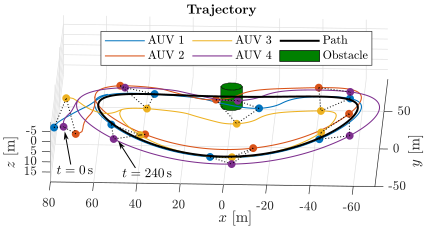
\includegraphics[width=0.75\textwidth]{figures/distr_NSB/sim_trajectory.pdf}
    \vspace{-4mm}
    \caption{The 3D trajectory of the AUVs. The markers represent the AUVs at times $t = 0, 40, \ldots, 240$ seconds. The dotted lines represent the communications graph.}
    \label{fig:distr_NSB_sim_trajectory}
\end{figure}


The purpose of this simulation is to demonstrate that the path-following, formation-keeping, and consensus errors of the continuous-time scheme converge to zero.
To satisfy the assumptions of Lemma~\ref{lemma2}, the consensus gain $c_s$ must be greater than $\frac{2 U_d k_s}{\lambda_2} = 0.65$. We choose $c_s = c_p = 1$.
To test the obstacle avoidance scheme, we place a static obstacle at $\mat{p}_o = \inlinevector{0, 40}$ with radius $r_o = \SI{5}{\meter}$.
The minimum cone $\alpha_{\min}$ is set to $2$ degrees, and the formation radius update gain is $k_r = 0.1$.

The results are shown in \figref{fig:distr_NSB_simulation}.
\figref{fig:distr_NSB_sim_trajectory} shows the 3D trajectory of the \glspl{auv}. We can see that the \glspl{auv} converge to their desired formation while avoiding the obstacle represented by the green cylinder.
\figref{fig:distr_NSB_sim_errors} shows the path-following and formation-keeping errors. Initially, these errors exponentially converge to zero. When the obstacle avoidance scheme is activated, the path-following errors start diverging, as the \gls{los} velocity enters the collision cone. After the vehicles successfully avoid the obstacle, the errors again converge exponentially to zero.
\figref{fig:distr_NSB_sim_distance} shows the distance between the \glspl{auv} and the obstacle. We can see that the distance is always greater than $r_o$.
Figs.~\ref{fig:distr_NSB_sim_barycenter}, \ref{fig:distr_NSB_sim_parameter}, and \ref{fig:distr_NSB_sim_radius} show the errors of the consensus variables. These plots are in a logarithmic scale to demonstrate the exponential rate of convergence. Initially, the logarithmic error is clearly bounded by a decreasing straight line, demonstrating the exponential convergence. The norm of the error decreases by a factor of 10 approximately every 25 seconds. When obstacle avoidance is active, the errors start diverging but remain bounded. After avoiding the obstacle, the errors continue to decrease exponentially, but eventually, the convergence stagnates. We cannot expect that the errors continue to fall indefinitely due to numerical innacuracies, that come mostly from two sources: the inaccuracies in floating-point arithmetics and the tolerances of the ODE solver.

Note that although Section~\ref{sec:distr_NSB_closed_loop} presents stability proof for a simplified case of straight-line paths and vehicles with single-integrator dynamics, the simulation results show stability for curved paths and more complex vehicle models.

\subsection{Event-Triggered Consensus}

In this section, we test the event-triggered scheme proposed in Section~\ref{sec:distr_NSB_event_triggered}.
We choose the mixing gains $a_p = a_s = 0.4$, and the penalty gains: $b_p = 10^{-4}, b_s = 4$.

We compare our algorithm with an event-triggered cooperative path following algorithm proposed in \cite{praveen_cooperative_2018}.
In this algorithm, each vehicle follows its own desired path given by $\mat{p}_{d,i}(s) = \mat{p}_p(s) + \mat{R}_p(s) \mat{p}_{f, i}^f$.
Coordination is then achieved by running a consensus scheme on the path parameter.

The comparison was done using a Monte Carlo simulation.
We performed ten thousand simulations with randomly selected initial conditions and communication delays.
The initial positions of the \glspl{auv} ranged from $\inlinevector{60,-40,0}$ to $\inlinevector{140,40,15}$.
The initial orientations were specified in Euler angles, with a zero roll angle, a pitch angle from $-\frac{\pi}{8}$ to $\frac{\pi}{8}$, and a yaw angle from $0$ to $\pi$.
The initial linear velocities ranged from $\inlinevector{0.5, -0.2, -0.1}$ to $\inlinevector{1.5, 0.2, 0.1}$, and the initial angular velocities were zero.
The communication delays ranged from $0$ to $5$ seconds.

\begin{figure}[t]
    \centering
    \begin{subfigure}{0.475\textwidth}
        \input{figures/distr_NSB/comparison_parameter.tex}
        \caption{}
        \label{fig:distr_NSB_comparison_parameter}
        \vspace{-8.5mm}
    \end{subfigure}
    \begin{subfigure}{0.475\textwidth}
        \input{figures/distr_NSB/comparison_barycenter.tex}
        \caption{}
        \label{fig:distr_NSB_comparison_barycenter}
        \vspace{-8.5mm}
    \end{subfigure}
    \caption{Comparison between the proposed event-triggered distributed NSB algorithm and the cooperative path-following algorithm proposed in \cite{praveen_cooperative_2018}. The full lines represent the median, the colored areas represent the smallest and largest recorded value.}
    \label{fig:distr_NSB_comparison}
\end{figure}


\figref{fig:distr_NSB_comparison} shows the absolute value of the path parameter error and the norm of the path-following error.
Both errors are plotted in a logarithmic scale.
In terms of path parameter errors, both algorithms perform similarly.
In terms of path-following errors, the distributed \gls{nsb} algorithm is marginally better.

The communication requirements of the two algorithms are summarized in Table~\ref{tab:comparison}.
This table shows the minimum, maximum, and median of the period in-between transmissions ($\tau_t$), and the total number of transmissions in one simulation ($N_t$).
Here, we can see that distributed \gls{nsb} performs considerably better in comparison to the cooperative path following method, with longer periods in-between transmissions and a lower number of transmissions.

However, it is worth mentioning that the packets transmitted by the cooperative path following method are smaller than the \gls{nsb} packets.
Indeed, in the scheme proposed in \cite{praveen_cooperative_2018}, the \glspl{auv} only need to transmit the path parameter and its derivative.
In contrast, the \gls{nsb} packet consists of the estimates of path parameter, barycenter, radius of formation, and formation-keeping error.
In this context, the two algorithms present a trade-off between packet size and communication periods.

\begin{table}[ht]
    \centering
    \caption{Comparison of communication requirements.}
    \label{tab:comparison}
    \begin{tabular}[t]{c|c|c|c|c}
        \textbf{Method}                                & \textbf{Quantity} & \textbf{Minimum} & \textbf{Median} & \textbf{Maximum} \\ \hline
        \multirow{2}{23mm}{Distributed NSB}            & $\tau_t$          & 2.00             & 8.50            & 275.30  \\
                                                       & $N_t$             & 125              & 187             & 253     \\ \hline
        \multirow{2}{23mm}{Coordinated path following} & $\tau_t$          & 0.10             & 2.15            & 138.65  \\
                                                       & $N_t$             & 196              & 548             & 1064 
    \end{tabular}
\end{table}


\section{Experiments}
\label{sec:distr_NSB_experiments}
In this section, we present the results of field experiments we designed and executed to verify the effectiveness of the event-triggered distributed \gls{nsb} algorithm proposed in Section~\ref{sec:distr_NSB_event_triggered}.
The experiments were conducted in the fjord of Trondheim, Norway, near the Trondheim Biological Station, using two \glspl{lauv} as in \figref{fig:distr_NSB_LAUV}.

\begin{figure}[b]
    \centering
    \includegraphics[width = 0.6\columnwidth]{figures/distr_NSB/LAUV-Roald}
    \caption{Photo of one of the two \glspl{lauv} used in the reported field experiments, courtesy of \url{www.ntnu.edu/aur-lab/}.}
    \label{fig:distr_NSB_LAUV}
\end{figure}

To guarantee stable communications and accurate navigation, the vehicles were operating at the surface and communicating over WiFi.
The algorithm was implemented in C++, using the Unified Navigation Environment (DUNE) \cite{dune}.

The algorithm was tested in two scenarios: a \emph{nominal} scenario, \emph{i.e.,} formation path following without any obstacles, and a scenario with a static obstacle.
In both scenarios, the barycenter of the \glspl{auv} should follow the elliptic path
\begin{align}
    \mat{p}_p(s) &= \inlinevector{a \cos(s), b \sin(s), 0},& 
    a &= \SI{100}{\meter},& 
    b &= \SI{80}{\meter},
\end{align}
in the formation defined by
\begin{align}
    \mat{p}_{f, 1}^f &= \inlinevector{0, -25, 0}, &
    \mat{p}_{f, 2}^f &= \inlinevector{0, 25, 0}.
\end{align}
The reason for choosing a larger path and formation, compared to the simulations in Section~\ref{sec:distr_NSB_simulations}, was to reduce the risk of the \glspl{auv} colliding.
The obstacle was placed at $\mat{p}_o = \inlinevector{0, 80}$.
The remaining parameters were identical to the simulations.

\subsection{Nominal Scenario}
\begin{figure}[p]
    \centering
    \includegraphics[width = 0.5\columnwidth]{figures/distr_NSB/LAUV-Roald}
    \vspace*{-1mm}
    \caption{Photo of one of the two \glspl{lauv} used in the reported field experiments, courtesy of \url{www.ntnu.edu/aur-lab/}.}
    \label{fig:distr_NSB_LAUV}
    \vspace*{-10mm}
\end{figure}

\begin{figure}[p]
    \begin{minipage}{0.48\textwidth}
        \begin{subfigure}{\textwidth}
            \input{figures/distr_NSB/experiment_nominal_trajectory.tex}
            \vspace{-2mm}
            \caption{The trajectory of the AUVs. The markers represent the AUVs at times $t = 0, 60, \ldots, 420$ seconds.}
            \label{fig:distr_NSB_experiment_nominal_trajectory}
        \end{subfigure}

        \vspace{-1mm}

        \begin{subfigure}{\textwidth}
            \input{figures/distr_NSB/experiment_nominal_parameter.tex}
            \vspace{-3mm}
            \caption{The path parameter errors. The markers represent transmissions.}
            \label{fig:distr_NSB_experiment_nominal_parameter}
        \end{subfigure}
    \end{minipage}
    \hspace{\fill}
    \begin{minipage}{0.48\textwidth}

        \hspace*{\fill}
        \begin{subfigure}{\textwidth}
            \hspace*{-5mm}
            \input{figures/distr_NSB/experiment_nominal_errors.tex}
            \vspace{-3mm}
            \caption{The path-following and formation-keeping errors.}
            \label{fig:distr_NSB_experiment_nominal_errors}
        \end{subfigure}

        %\vspace{-4mm}

        \hspace*{\fill}
        \begin{subfigure}{\textwidth}
            \hspace*{-5mm}
            \input{figures/distr_NSB/experiment_nominal_barycenter.tex}
            \vspace{-3mm}
            \caption{The $x$- and $y$-components of barycenter estimate errors.}
            \label{fig:distr_NSB_experiment_nominal_barycenter}
        \end{subfigure}
    \end{minipage}

    \vspace*{-3mm}
    \caption{Results of a nominal experiment.}
    \label{fig:distr_NSB_experiment_nominal}
\end{figure}


The results are shown in \figref{fig:distr_NSB_experiment_nominal}.
\figref{fig:distr_NSB_experiment_nominal_trajectory} shows the trajectories of the \glspl{auv}, as estimated by their onboard navigation system.
The disturbances in the trajectories are caused by two factors: the sea loads (waves, currents, and wind), and the errors of the navigation system.
However, the exponential stability of the \gls{nsb} algorithm given by Theorem~\ref{thm_distr_NSB} provides some robustness towards these disturbances, \emph{c.f.,} \cite[Lemma 9.2]{khalil_nonlinear_2002}.
\figref{fig:distr_NSB_experiment_nominal_parameter} shows the path parameter errors and the event-triggered communications.
Initially, the vehicles need to communicate frequently, approximately every five seconds, because the barycenter estimates differ (as seen in \figref{fig:distr_NSB_experiment_nominal_barycenter}).
During this transient period, the path parameter estimates initially diverge before finally converging.
After convergence, the communication period increases to over 100 seconds.
Note that the barycenter estimate errors in \figref{fig:distr_NSB_experiment_nominal_barycenter} converge to a common value but not to zero.
This behavior is caused by the aforementioned disturbances acting on the vehicles.
\figref{fig:distr_NSB_experiment_nominal_errors} shows the formation-keeping and path-following errors.
Due to the disturbances and event-triggered communications, these errors do not converge to zero but rather to a small area near zero.

\subsection{Scenario with a Static Obstacle}
\begin{figure}[p]
    \begin{minipage}{0.48\textwidth}
        \begin{subfigure}{\textwidth}
            \input{figures/distr_NSB/experiment_obstacle_trajectory.tex}
            \vspace{-3mm}
            \caption{The trajectory of the AUVs. The markers represent the AUVs at times $t = 0, 60, \ldots, 420$ seconds.}
            \label{fig:distr_NSB_experiment_obstacle_trajectory}
        \end{subfigure}

        %\vspace{-4mm}

        \hspace*{\fill}
        \begin{subfigure}{\textwidth}
            \hspace*{-3mm}
            \input{figures/distr_NSB/experiment_obstacle_errors.tex}
            \vspace{-8mm}
            \caption{The path-following and formation-keeping errors. The green area represents the time when obstacle avoidance is active.}
            \label{fig:distr_NSB_experiment_obstacle_errors}
        \end{subfigure}
    \end{minipage}
    \hspace{\fill}
    \begin{minipage}{0.48\textwidth}

        \hspace*{\fill}
        \begin{subfigure}{\textwidth}
            \hspace*{-3mm}
            \input{figures/distr_NSB/experiment_obstacle_parameter.tex}
            \vspace{-8mm}
            \caption{The path parameter errors. The markers represent transmissions.}
            \label{fig:distr_NSB_experiment_obstacle_parameter}
        \end{subfigure}

        %\vspace{-4mm}

        \hspace*{\fill}
        \begin{subfigure}{\textwidth}
            \hspace*{-3mm}
            \input{figures/distr_NSB/experiment_obstacle_barycenter.tex}
            \vspace{-8mm}
            \caption{The $x$- and $y$-components of barycenter estimate errors.}
            \label{fig:distr_NSB_experiment_obstacle_barycenter}
        \end{subfigure}


        %\vspace{-4mm}

        \hspace*{\fill}
        \begin{subfigure}{\textwidth}
            \input{figures/distr_NSB/experiment_obstacle_distance.tex}
            \vspace{-8mm}
            \caption{The distance between the AUVs and the obstacle.}
            \label{fig:distr_NSB_experiment_obstacle_distance}
        \end{subfigure}

        %\vspace{-4mm}

        \hspace*{\fill}
        \begin{subfigure}{\textwidth}
            \input{figures/distr_NSB/experiment_obstacle_radius.tex}
            \vspace{-8mm}
            \caption{The error between the estimated and true formation radius.}
            \label{fig:distr_NSB_experiment_obstacle_radius}
        \end{subfigure}
    \end{minipage}

    \caption{Experiment with a static obstacle.}
    \label{fig:distr_NSB_experiment_obstacle}
\end{figure}


The results are shown in \figref{fig:distr_NSB_experiment_obstacle}.
In general, the results are similar to the nominal scenario, so we will only highlight the differences.
The path-following errors in \figref{fig:distr_NSB_experiment_obstacle_errors} diverge when obstacle avoidance is active.
As previously mentioned, this behavior is caused by the fact that the vehicles cannot stay on the desired path while avoiding the obstacle.
The estimate errors in Figs.~\ref{fig:distr_NSB_experiment_obstacle_parameter} and \ref{fig:distr_NSB_experiment_obstacle_barycenter} behave similarly to the nominal case.
As shown in \figref{fig:distr_NSB_experiment_obstacle_distance}, the distance between the \glspl{auv} and the obstacle is always greater than $r_o$.
\figref{fig:distr_NSB_experiment_obstacle_radius} shows the errors between the estimated and true formation radius.
Note that the formation radius errors are connected to the barycenter estimates.
A wrong barycenter estimate may lead to both overestimation and underestimation of the formation radius.
Despite these uncertainties, the \glspl{auv} still manage to perform all control goals safely.


\part{Hand Position and its Applications}
\label{part:hand_position}

\chapter{Hand Position for Underactuated Underwater Vehicles}
\label{chap:handpos_definition}

This chapter motivates and defines the hand position concept.
Compared to previous works that utilize this concept, our approach works on six-degree-of-freedom vehicles and does not introduce singularities.
By choosing the hand position as the output of the controlled system, we can apply output feedback linearization to simplify the dynamics of the vehicle.
Specifically, we can then transform the six-degree-of-freedom nonlinear underactuated vehicle model into a double integrator.
This transformation enables the use of numerous control strategies that could otherwise not be used on nonholonomic or underactuated vehicles.
The contents of this chapter are based on \cite{matous_trajectory_2023}.
In \cite{matous_distributed_2023}, we proposed and analyzed controllers that solve the path-following and trajectory-tracking problems.
This chapter presents an analysis of a generic hand position-based controller.

\section{Introduction}

This thesis studies slender torpedo-shaped \acrfullpl{auv} with a propeller that provides forward (surge) thrust, and fins that provide torque.
The configuration of actuators means that \glspl{auv} are \emph{underactuated}, as we cannot directly control the lateral (sway and heave) velocities.
The underactuated nature of \glspl{auv} makes them difficult to control.
In addition, \glspl{auv} are subject to constant disturbances caused by the waves and ocean currents, commonly referred to as sea loads.

In this chapter, we propose to use the \emph{hand position} concept to control the AUV.
The hand position is a point located a given distance in front of the neutral point along the vehicle's $x$-axis (see \figref{fig:handpos_def_motivation}b for an illustration).
The concept was first introduced in \cite{pomet_hand-position_1992} to stabilize nonholonomic vehicles with unicycle dynamics.
Later, it was applied to control formations of unicycles \cite{lawton_hand-position-formation_2003}.
The concept was then extended to marine vehicles moving in the horizontal plane \cite{paliotta_trajectory_2019}, and two- and three-dimensional Euler-Lagrange-like systems \cite{cai_hand-position-rigidity-planar_2015,li_hand-position-rigidity-3d_2021}.

\begin{figure}[t]
    \centering
    \def\svgwidth{0.75\textwidth}
    \import{figures/handpos_def}{motivation.pdf_tex}
    \caption{Illustration of (a) the traditional trajectory tracking and path following controllers, and (b) the proposed hand position-based controller. The dashed line represents the body-fixed $x$-axis.}
    \label{fig:handpos_def_motivation}
\end{figure}

There are two main advantages to using the hand position concept.
The first advantage stems from the applications of AUVs.
The aim of many scientific missions is to scan a given area using a sensor attached to the AUV.
Since the position of the sensor typically does not coincide with the neutral point, there may be a significant offset between the sensor and the desired trajectory, caused by the sea loads (see \figref{fig:handpos_def_motivation}a).
In some cases, the hand position can be chosen such that it coincides with the position of the sensor, allowing to scan the area more accurately.
The second advantage is that if we choose the hand position as the output of our system, it is possible to transform the nonlinear underactuated vehicle model to a double integrator, using output feedback linearization.
This allows us to apply advanced control strategies, \emph{e.g.,} various consensus algorithms \cite{cai_hand-position-rigidity-planar_2015,li_hand-position-rigidity-3d_2021,lawton_hand-position-formation_2003,restrepo_tracking-formation_2022} that cannot be directly used on nonholonomic or underactuated vehicles.

Note that the three-dimensional Euler-Lagrange-like system used in \cite{li_hand-position-rigidity-3d_2021} does not accurately represent AUVs, since it does not consider the Coriolis and centripetal effects or the restoring forces (gravity and buoyancy).
Furthermore, the model in \cite{li_hand-position-rigidity-3d_2021} has five \acrfullpl{dof}: three position coordinates, pitch angle, and yaw angle.
The use of Euler angles inherently introduces singularities into the system.

The goal of this paper is thus to further extend the hand position concept to AUVs moving in three dimensions.
We employ a more realistic AUV model than in \cite{li_hand-position-rigidity-3d_2021}. We model the full 6DOF motion and use rotation matrices to describe the orientation of the vehicle, thus avoiding singularities.
Using Lyapunov analysis, we show the sufficient conditions for boundedness of the internal dynamics, \emph{i.e.,} the orientation and the angular velocities, for a generic hand position-based controller.


\chapter{Trajectory Tracking and Path Following using the Hand Position Concept}
\label{chap:handpos_trajectory}

This chapter presents hand position-based trajectory-tracking and path-following controllers for underactuated underwater vehicles.
Using Lyapunov analysis, we show that the proposed controllers exponentially track the desired trajectory or path, while the angular velocities of the vehicle remain bounded.
The theoretical results are verified both in numerical simulations and experiments.
The contents of this chapter are based on \cite{matous_trajectory_2023}.

The chapter is organized as follows.
Sections~\ref{sec:handpos_trajectory_trajectory_tracking} and \ref{sec:handpos_trajectory_path_following} present and analyze the trajectory-tracking and the path-following controller, respectively.
Sections~\ref{sec:handpos_trajectory_simulations} and \ref{sec:handpos_trajectory_experiments} show the results of numerical simulations and experiments, respectively.

\section{Trajectory Tracking}
\label{sec:handpos_trajectory_trajectory_tracking}
In this section, we propose a control law for tracking a predefined trajectory.
Let $\bs{\xi}_{1, d}$ represent the desired trajectory, and let $\bs{\xi}_{2, d} = \dot{\bs{\xi}}_{1, d}$.
We assume that there exist $\bs{\xi}_{2, d, \max}$ and $\dot{\bs{\xi}}_{2, d, \max}$ such that
\begin{align}
    \norm{\ocean} &< \norm{\bs{\xi}_{2, d}} \leq \bs{\xi}_{2, d, \max}, &
    \norm{\dot{\bs{\xi}}_{2, d}} \leq \dot{\bs{\xi}}_{2, d, \max}.
\end{align}

The goal of trajectory tracking is to control the vehicle such that $\mat{x}_1$ converges to $\bs{\xi}_{1, d}$.
To achieve the goal, we define the following error states
\begin{subequations}
    \begin{align}
        \tilde{\mat{x}}_1 &= \mat{x}_1 - \bs{\xi}_{1, d}, \\
        \tilde{\mat{x}}_2 &= \mat{x}_2 - \bs{\xi}_{2, d}, \\
        \tilde{\mat{x}}_I &= \int_{0}^t \tilde{\mat{x}}_1(s)\, {\rm d}s,
    \end{align} \label{eq:handpos_trajectory_error_states}
\end{subequations}
and choose the following PID controller
\begin{equation}
    \bs{\mu} = -k_p \tilde{\mat{x}}_1 - k_d \tilde{\mat{x}}_2 - k_I \tilde{\mat{x}}_I + \dot{\bs{\xi}}_{2, d}, \label{eq:handpos_trajectory_external_controller}
\end{equation}

\noindent where $k_p$, $k_d$, and $k_I$ are positive gains chosen such that the matrix
\begin{equation}
    \mat{H}_{\xi}
    =
    \begin{bmatrix}
        \mat{O}_{3 \times 3} & \mat{I}_{3} & \mat{O}_{3 \times 3} \\ \mat{O}_{3 \times 3} & \mat{O}_{3 \times 3} & \mat{I}_{3} \\ -k_I \mat{I}_{3} & -k_p \mat{I}_{3} & -k_d \mat{I}_{3}
    \end{bmatrix} \label{eq:handpos_trajectory_H_xi}
\end{equation}
is Hurwitz.

\subsection{Closed-Loop Analysis}
In this section, we investigate the closed-loop dynamics of the system \eqref{eq:handpos_def_hand_position_dynamics} with the control law \eqref{eq:handpos_trajectory_external_controller}.
We begin by defining an additional change of coordinates:
\begin{subequations}
    \begin{align}
        \tilde{\bs{\xi}}_1 &= \tilde{\mat{x}}_1, \\
        \tilde{\bs{\xi}}_2 &= \tilde{\mat{x}}_2 + \ocean, \\
        \tilde{\bs{\xi}}_I &= \tilde{\mat{x}}_I - \frac{k_d}{k_I}\ocean.
    \end{align} \label{eq:handpos_trajectory_hand_transform_CL}
\end{subequations}
This change is necessary to transform the equilibrium of the closed-loop system to the origin, as the error states $\tilde{\mat{x}}_2$ and $\tilde{\mat{x}}_I$ defined in \eqref{eq:handpos_trajectory_external_controller} do not converge to zero.

For convenience, we will also define a concatenated state vector
\begin{equation}
    \bs{\Xi}\T = \left[{\tilde{\bs{\xi}}}_I\T, {\tilde{\bs{\xi}}}_1\T, {\tilde{\bs{\xi}}}_2\T\right].
    \label{eq:handpos_trajectory_XI}
\end{equation}
Differentiating \eqref{eq:handpos_trajectory_XI} with respect to time and substituting the external dynamics \eqref{eq:handpos_def_x_1_dot_transformed}--\eqref{eq:handpos_def_x_2_dot_transformed} and the control law \eqref{eq:handpos_trajectory_external_controller}, we get
\begin{equation}
    \dot{\bs{\Xi}} = \mat{H}_{\xi} \bs{\Xi}. \label{eq:handpos_trajectory_external_dynamics}
\end{equation}

\begin{prop}
    \label{prop:handpos_trajectory_trajectory_tracking}
    The origin $\bs{\Xi} = \mat{0}$ is a \acrfullpl{ges} equilibrium point of \eqref{eq:handpos_trajectory_external_dynamics}.
    Consequently, $\mat{x}_1$, $\mat{x}_2$, and $\tilde{\mat{x}}_I$ exponentially converge to $\bs{\xi}_{1, d}$, $\bs{\xi}_{2, d} - \ocean$, and $k_I/k_d\,\ocean$, respectively.

    Moreover, let us define $a_x, \Bar{\alpha}_y, \Bar{\alpha}_z$ in accordance with \eqref{eq:handpos_def_a_bounds}.
    The internal dynamics are ultimately bounded if $a_x, \Bar{\alpha}_y, \Bar{\alpha}_z > 0$.
\end{prop}
\begin{proof}
    Since the matrix $\mat{H}_{\xi}$, defined in \eqref{eq:handpos_trajectory_H_xi} is Hurwitz by design, we can conclude that the external dynamics are \glspl{ges}, and $\tilde{\bs{\xi}}_1$, $\tilde{\bs{\xi}}_2$, and $\tilde{\bs{\xi}}_I$ exponentially converge to zero.

    From \eqref{eq:handpos_trajectory_error_states}, we can conclude that if $\tilde{\bs{\xi}}_1$ exponentially converges to zero, then the hand position $\mat{x}_1$ exponentially converges towards the desired trajectory $\bs{\xi}_{1, d}$.
    Similarly, if $\tilde{\bs{\xi}}_2$ converges to zero, then the relative hand velocity $\mat{x}_2$ converges to $\bs{\xi}_{2, d} - \ocean$.
    Moreover, if $\tilde{\bs{\xi}}_I$ converges to zero, then the integral state $\tilde{\mat{x}}_I$ converges to $k_I/k_d\,\ocean$.
    Consequently, the integral state provides an estimate of the ocean current.

    Moreover, because the external dynamics are stable, the error states $\tilde{\mat{x}}_1$, $\tilde{\mat{x}}_2$, and $\tilde{\mat{x}}_I$ are bounded.
    Consequently, the control input $\bs{\mu}$ is bounded.
    Therefore, if $a_x, \Bar{\alpha}_y, \Bar{\alpha}_z > 0$, then all assumptions of Lemma~\ref{lemma:handpos_def_ultimate_boundedness} are satisfied, and the internal dynamics are ultimately bounded.
\end{proof}

\subsection{Straight-Line Trajectory Tracking}
\label{sec:handpos_trajectory_straight_line_trajectory}
In this section, we will focus on the special case when $\bs{\xi}_{2, d}$ is constant, and the vehicle is thus tracking a straight line.
The purpose of this section is to demonstrate that in this special case, we can prove that both the external and internal dynamics are exponentially stable.
First, let us present the necessary definitions and assumptions.

\begin{dfn}
    Two vectors $\mat{a}, \mat{b} \in \mathbb{R}^3$ are aligned if there exists $k \in \mathbb{R}$ such that $\mat{a} = k\mat{b}$.
    Equivalently, $\mat{a}$ and $\mat{b}$ are aligned if $\mat{a} \times \mat{b} = \mat{0}_3$.
    \label{dfn:aligned}
\end{dfn}
\begin{asm}
    The distance between the centers of gravity and buoyancy, $z_{gb}$, is positive, and the vector $\bs{\xi}_{2, d, r} = (\bs{\xi}_{2, d} - \ocean)$ is not aligned with $\mat{e}_3$.
    \label{asm:straight_line_trajectory}
\end{asm}
\begin{rmk*}
    From \eqref{eq:gravity}, one can verify that if $z_{gb}$ is positive, then the restoring forces stabilize the vehicle's roll angle around zero.
    Consequently, most commercial \glspl{auv} are designed so that $z_{gb} > 0$.
    The second part of Assumption~\ref{asm:straight_line_trajectory} can be satisfied by choosing an appropriate reference trajectory.
\end{rmk*}

We begin by finding the equilibria of the closed-loop system.
Since the external dynamics is a linear system, $\bs{\Xi} = \mat{0}_9$ is the only equilibrium.
From \eqref{eq:handpos_def_R_dot_CL}, we can conclude that $\dot{\mat{R}} = \mat{O}_{3 \times 3}$ if and only if $\bs{\omega} = \mat{0}_3$.
Substituting $\bs{\Xi} = \mat{0}_9$ and $\bs{\omega} = \mat{0}_3$ into \eqref{eq:handpos_def_omega_dot_CL} yields
\begin{equation}
    %\begin{split}
        \dot{\bs{\omega}} = \Bar{\mat{L}} \times \left(\mathcal{D}_{\bvel}(\vel_r) + \mathcal{C}_{\bvel}(\vel_r)\right) 
        - \left(\Bar{\mat{L}}\mat{L}\T\right) \left(\mathcal{D}_{\bs{\omega}}(\vel_r) + \mat{M}_{22}^{\prime}\left(Wz_{gb} \mat{e}_3 \times \mat{R}\T \mat{e}_3\right)\right).
    %\end{split}
    \label{eq:handpos_trajectory_omega_dot_SS}
\end{equation}
Note that the right-hand-side of \eqref{eq:handpos_trajectory_omega_dot_SS} has the following form
\begin{equation}
    \dot{\bs{\omega}} = \Bar{\mat{L}} \times \mat{a} + \left(\Bar{\mat{L}}\mat{L}\T\right) \mat{b},
\end{equation}
where $\mat{a} = \inlinevector{a_1, a_2, a_3}$, $\mat{b} = \inlinevector{b_1, b_2, b_3}$ are vectors in $\mathbb{R}^3$.
From the definition of $\mat{L}$ and $\Bar{\mat{L}}$, the following two equalities hold for any $\mat{a}$ and $\mat{b}$:
\begin{align}
    \Bar{\mat{L}} \times \mat{a} &= \frac{1}{h} \inlinevector{0, -a_3, a_2}, &
    \left(\Bar{\mat{L}}\mat{L}\T\right) \mat{b} &= \inlinevector{b_1, 0, 0}.
\end{align}
Consequently, $\dot{\bs{\omega}}$ is zero if and only if both terms of the right-hand-side of \eqref{eq:handpos_trajectory_omega_dot_SS} are zero.

The first term is zero only if $\left(\mathcal{D}_{\bvel}(\vel_r) + \mathcal{C}_{\bvel}(\vel_r)\right)$ is aligned with $\mat{e}_1$.
In other words, there exists $k \in \mathbb{R}$ such that
\begin{equation}
    \mathcal{D}_{\bvel}(\vel_r) + \mathcal{C}_{\bvel}(\vel_r) = k \mat{e}_1. \label{eq:handpos_trajectory_steady_state_condition_1}
\end{equation}
Substituting \eqref{eq:handpos_def_ode_components} into \eqref{eq:handpos_trajectory_steady_state_condition_1}, we get the following equation
\begin{equation}
    \begin{bmatrix}
        \frac{d_{11}}{m_{11}}\,u_r \\
        \frac{m_{66}d_{22} - d_{62}m_{26} + m_{26}\left(m_{11} - m_{22}\right)u_r}{m_{22}m_{66} - m_{26}^2}\,v_r \\
        \frac{m_{55}d_{33} - d_{53}m_{35} - m_{35}\left(m_{11} - m_{33}\right)u_r}{m_{33}m_{55} - m_{35}^2}\,w_r
    \end{bmatrix}
     = \begin{bmatrix}
        k \\ 0 \\ 0
     \end{bmatrix}, \label{eq:handpos_trajectory_steady_state_condition_1_expanded}
\end{equation}
which has at least one solution given by
\begin{equation}
    \inlinevector{u_r, v_r, w_r} = \frac{m_{11}}{d_{11}} k \mat{e}_1. \label{eq:handpos_trajectory_steady_state_solution_1}
\end{equation}
Note that if
\begin{equation}
    \frac{d_{62}m_{26} - m_{66}d_{22}}{m_{26}\left(m_{11} - m_{22}\right)}
    \neq
    \frac{m_{55}d_{33} - d_{53}m_{35}}{m_{35}\left(m_{11} - m_{33}\right)},
    \label{eq:handpos_trajectory_inequality}
\end{equation}
then \eqref{eq:handpos_trajectory_steady_state_solution_1} is the only solution of \eqref{eq:handpos_trajectory_steady_state_condition_1_expanded}.
From \eqref{eq:handpos_def_nu_r_transformed}, the steady-state linear velocities must also satisfy
\begin{align}
    \bvel_r &= \mat{R}\T \bs{\xi}_{2, d, r}& &\implies& \norm{\bvel_r} &= \norm{\bs{\xi}_{2, d, r}}. \label{eq:handpos_trajectory_steady_state_condition_2}
\end{align}
Combining \eqref{eq:handpos_trajectory_steady_state_solution_1} and \eqref{eq:handpos_trajectory_steady_state_condition_2} gives us two possible steady-state linear velocities
\begin{equation}
    \bvel_r = \pm \norm{\bs{\xi}_{2, d, r}}\,\mat{e}_1,
\end{equation}
which leads to the following condition on the steady-state orientation
\begin{equation}
    \mat{R} \mat{e}_1 = \pm \frac{\bs{\xi}_{2, d, r}}{\norm{\bs{\xi}_{2, d, r}}}. \label{eq:handpos_trajectory_steady_state_R_1}
\end{equation}
This condition does not uniquely define the steady-state orientation.
Indeed, in terms of Euler angles, \eqref{eq:handpos_trajectory_steady_state_R_1}, defines the steady-state yaw and pitch angles.
%Note that the steady-state pitch angle is $\pm \frac{\pi}{2}$ radians only if $\bs{\xi}_{2, d, r}$ is aligned with $\mat{e}_3$.
An additional condition on the steady-state orientation comes from the second term in \eqref{eq:handpos_trajectory_omega_dot_SS}.
This term is zero if
\begin{equation}
    \mat{e}_1\T \left(Wz_{gb} \mat{e}_3 \times \mat{R}\T \mat{e}_3\right) = 0. \label{eq:handpos_trajectory_steady_state_R_2}
\end{equation}
If Assumption~\ref{asm:straight_line_trajectory} holds, then \eqref{eq:handpos_trajectory_steady_state_R_2} is equivalent to
\begin{equation}
    \sin\phi = 0,
\end{equation}
where $\phi \in [0, 2\pi)$ is the steady-state roll angle.
Consequently, \eqref{eq:handpos_trajectory_steady_state_R_1} and \eqref{eq:handpos_trajectory_steady_state_R_2} result in four distinct steady-state orientations.
Intuitively, the vehicle can have positive or negative surge velocity, and a roll angle of zero or $\pi$ radians.
These four equilibria are illustrated in Figure~\ref{fig:equilibria}.

\begin{figure}[tb]
    \centering
    \def\svgwidth{0.48\textwidth}
    \import{figures/handpos_trajectory}{auv_equilibria.pdf_tex}
    \caption{Illustration of the four equilibria. (a) Positive surge velocity, zero roll angle. (b) Positive surge velocity, $\pi$ radians roll. (c) Negative surge velocity, zero roll angle. (d) Negative surge velocity, $\pi$ radians roll.}
    \label{fig:equilibria}
\end{figure}

In the remainder of this section, we will analyze the equilibrium in which the vehicle has a positive surge velocity, and the roll angle is zero, \emph{c.f.,} Figure~\ref{fig:equilibria}a.
Let $\mat{R}_0$ denote the steady-state orientation.
We define the orientation error, $\bs{\delta}$, as
\begin{equation}
    \bs{\delta} = {\rm logm}\left(\mat{R}_0\T\,\mat{R}\right),
    \label{eq:handpos_trajectory_delta}
\end{equation}
where ${\rm logm}: SO(3) \mapsto \ball[3]{\pi}$ is the matrix logarithm \cite{iserles_lie_2000}, and introduce the following change of coordinates
\begin{align}
    \tilde{\bs{\xi}}_I^{\prime} &= \mathbf{R}\T\,\tilde{\bs{\xi}}_I, &
    \tilde{\bs{\xi}}_1^{\prime} &= \mathbf{R}\T\,\tilde{\bs{\xi}}_1, &
    \tilde{\bs{\xi}}_2^{\prime} &= \mathbf{R}\T\,\tilde{\bs{\xi}}_2.
\end{align}
The motivation behind the change of coordinates is to simplify the relation between the external dynamics and $\bvel_r$.
From, \eqref{eq:handpos_def_nu_r_transformed}, $\bvel_r$ is given by
\begin{equation}
    \begin{split}
    \bvel_r &= \mathbf{R}\T\left(\tilde{\bs{\xi}}_2 + \bs{\xi}_{2, d} - \ocean\right) - \bs{\omega} \times \mat{L} \\
        &= \tilde{\bs{\xi}}_2^{\prime} + {\rm expm}(\bs{\delta})\T \norm{\bs{\xi}_{2_{d,r}}}\mat{e}_1 - \bs{\omega} \times \mat{L},
    \end{split}
\end{equation}
where ${\rm expm}: \ball[3]{\pi} \mapsto SO(3)$ is the inverse of ${\rm logm}$.

The complete closed-loop system is then given by
\begin{subequations}
    \begin{align}
        \dot{\tilde{\bs{\xi}}}_I^{\prime} &= \tilde{\bs{\xi}}_1^{\prime} - \bs{\omega} \times \tilde{\bs{\xi}}_I^{\prime}, \\
        \dot{\tilde{\bs{\xi}}}_1^{\prime} &= \tilde{\bs{\xi}}_2^{\prime} - \bs{\omega} \times \tilde{\bs{\xi}}_1^{\prime}, \\
        \dot{\tilde{\bs{\xi}}}_2^{\prime} &= -k_I \tilde{\bs{\xi}}_I^{\prime} - k_p \tilde{\bs{\xi}}_1^{\prime} - k_d \tilde{\bs{\xi}}_2^{\prime} - \bs{\omega} \times \tilde{\bs{\xi}}_2^{\prime}, \\
        \dot{\bs{\delta}} &= \bs{\omega}, \\
        \dot{\bs{\omega}} &= \Bar{\mat{L}} \times \bigg(-k_I \tilde{\bs{\xi}}_I^{\prime} - k_p \tilde{\bs{\xi}}_1^{\prime} - k_d \tilde{\bs{\xi}}_2^{\prime} + \mathcal{D}_{\bvel}(\vel_r) + \mathcal{C}_{\bvel}(\vel_r) \nonumber \\
        &\qquad \qquad - \bs{\omega} \times \left(\tilde{\bs{\xi}}_2^{\prime} + {\rm expm}(\bs{\delta})\T \norm{\bs{\xi}_{2_{d,r}}}\mat{e}_1\right)\bigg) \nonumber \\
        &\quad - \left(\Bar{\mat{L}}\mat{L}\T\right) \left(\mathcal{D}_{\bs{\omega}}(\vel_r) + \mat{M}_{22}^{\prime}\left(Wz_{gb} \mat{e}_3 \times \mathbf{R}\T \mat{e}_3\right)\right).
    \end{align}
\end{subequations}
Next, we define a vector $\mat{z}\T = \left[{\tilde{\bs{\xi}}_I^{\prime\,{\rm T}}}, {\tilde{\bs{\xi}}_1^{\prime\,{\rm T}}}, {\tilde{\bs{\xi}}_2^{\prime\,{\rm T}}}, \bs{\delta}\T, \bs{\omega}\T\right]$ and a function $f$ such that $\dot{\mat{z}} = f(\mat{z})$.
Let $\mat{J}$ denote the Jacobian of $f(\mat{z})$, evaluated at $\mat{z} = \mat{0}$.
$\mat{J}$ is given by

\begin{equation}
    \mat{J} \!=\! \begin{bmatrix}
        \mat{O}_{3 \times 3} & \mat{I}_{3} & \mat{O}_{3 \times 3} & \mat{O}_{3 \times 3} & \mat{O}_{3 \times 3} \\
        \mat{O}_{3 \times 3} & \mat{O}_{3 \times 3} & \mat{I}_{3} & \mat{O}_{3 \times 3} & \mat{O}_{3 \times 3} \\
        -k_I \mat{I}_{3}\!\!\! & -k_p \mat{I}_{3}\!\!\! & -k_d \mat{I}_{3}\!\!\!\! & \mat{O}_{3 \times 3} & \mat{O}_{3 \times 3} \\
        \mat{O}_{3 \times 3} & \mat{O}_{3 \times 3} & \mat{O}_{3 \times 3} & \mat{O}_{3 \times 3} & \mat{I}_{3} \\
        \mat{J}_{\bs{\xi}_I} & \mat{J}_{\bs{\xi}_1} & \mat{J}_{\bs{\xi}_2} & \mat{J}_{\bs{\delta}} & \mat{J}_{\bs{\omega}}
    \end{bmatrix}, \label{eq:handpos_trajectory_jacobian}
\end{equation}
where
\begin{subequations}
    \begin{align}
        \mat{J}_{\bs{\xi}_I} &= -\mat{S}\left(\frac{k_I}{h}\mat{e}_1\right), &
        \mat{J}_{\bs{\xi}_1} &= -\mat{S}\left(\frac{k_p}{h}\mat{e}_1\right), \\
        \mat{J}_{\bs{\xi}_2} &= \begin{bmatrix}
            0 & 0 & 0 \\
            0 & 0 & {\Xi}_{23} \\
            0 & {\Xi}_{32} & 0
        \end{bmatrix}, &
        \mat{J}_{\bs{\omega}} &= - \begin{bmatrix}
            \Omega_1 & 0 & 0 \\
            0 & \Omega_2 & 0 \\
            0 & 0 & \Omega_3
        \end{bmatrix} \\            
        %{\rm diag}\left(\Omega_1, \Omega_2, \Omega_3\right), \\
        \mat{J}_{\bs{\delta}} &= \mathrlap{\begin{bmatrix}
            -\Delta_1\cos\theta & 0 & \Delta_1\sin\theta \\
            0 & -\Delta_2 & 0 \\
            0 & 0 & -\Delta_3
        \end{bmatrix}.}            
    \end{align}
    \label{eq:handpos_trajectory_jacobian_blocks}
\end{subequations}
where $\theta$ is the steady-state pitch angle.
The components of $\mat{J}_{\bs{\xi}_2}$, $\mat{J}_{\bs{\omega}}$, and $\mat{J}_{\bs{\delta}}$ are shown in Appendix~\ref{app:jacobian}.

\begin{prop}
    The point $\mat{z} = \mat{0}_{15}$ is a (locally) exponentially stable equilibrium point of $\dot{\mat{z}} = f(\mat{z})$ if Assumption~\ref{asm:straight_line_trajectory} holds, and all $\Delta_i$ and $\Omega_i$ for $i \in \{1,2,3\}$ are positive.
    \label{prop:straight_line_trajectory}
\end{prop}
\begin{proof}
    Using the indirect Lyapunov method, the system is locally exponentially stable if $\mat{J}$ is Hurwitz.
    Let us define
    \begin{align}
        \mat{J}_{21}\! &= \!\begin{bmatrix}
            \mat{O}_{3 \times 3}\!\! & \mat{O}_{3 \times 3}\!\! & \mat{O}_{3 \times 3} \\
            \mat{J}_{\bs{\xi}_I} & \mat{J}_{\bs{\xi}_1} & \mat{J}_{\bs{\xi}_2}
        \end{bmatrix}, &
        \mat{J}_{22}\! &= \!\begin{bmatrix}
            \mat{O}_{3 \times 3}\!\! & \mat{I}_{3} \\
            \mat{J}_{\delta} & \mat{J}_{\omega}
        \end{bmatrix}\!.
    \end{align}
    The matrix $\mat{J}$ can then be written in the following form
    \begin{equation}
        \mat{J} = \begin{bmatrix}
            \mat{H}_{\xi} & \mat{O}_{9 \times 6} \\
            \mat{J}_{21} & \mat{J}_{22}
        \end{bmatrix}.
    \end{equation}
    Due to its block triangular structure, the eigenvalues of $J$ are equal to the union of eigenvalues of $\mat{H}_{\xi}$ and $\mat{J}_{22}$.
    Note that $\mat{H}_{\xi}$ is Hurwitz by design.
    Furthermore, the eigenvalues of $\mat{J}_{22}$, $\lambda_1, \ldots, \lambda_6$ are given by
    \begin{subequations}
        \begin{align}
            \lambda_1, \lambda_2 &= -\frac{\Omega_{1}}{2} \pm \frac{\sqrt{{\Omega_{1}}^2-4\,\Delta_{1}\cos\theta_0}}{2}, \\
            \lambda_3, \lambda_4 &= -\frac{\Omega_{2}}{2} \pm \frac{\sqrt{{\Omega_{2}}^2-4\,\Delta_{2}}}{2}, \\
            \lambda_5, \lambda_6 &= -\frac{\Omega_{3}}{2} \pm \frac{\sqrt{{\Omega_{3}}^2-4\,\Delta_{3}}}{2}.
        \end{align}
    \end{subequations}
    If Assumption~\ref{asm:straight_line_trajectory} holds, then the steady-state pitch angle satisfies $\abs{\theta} < \pi/2$.
    Therefore, the real part of $\lambda_1, \ldots, \lambda_6$ is strictly negative if Assumption~\ref{asm:straight_line_trajectory} holds and all $\Delta_i$ and $\Omega_i$ for $i \in \{1,2,3\}$ are positive.
\end{proof}

\begin{rmk*}
    For surface vessels, it has been shown that a similar controller can achieve almost global asymptotic stability \cite{paliotta_trajectory_2019}.
    For underwater vehicles, proving almost global stability is complicated.
    It can be shown that vehicles with rotational symmetry around the $x$-axis violate inequality \eqref{eq:handpos_trajectory_inequality}.
    Since most commercial AUVs have a cylindrical shape, this type of symmetry is common among underwater vehicles.
    If a vehicle violates inequality \eqref{eq:handpos_trajectory_inequality}, then there exists a subspace of unstable equilibria in addition to the four previously described equilibrium points, making almost global results impossible.
\end{rmk*}

\section{Path Following}
\label{sec:handpos_trajectory_path_following}
In this section, we present a path-following controller based on the hand position concept.
Let $s$ be the path parameter, $\mat{p}_p: \mathbb{R} \mapsto \mathbb{R}^{3}$ the parametrization of the desired path, and $U_d > 0$ the desired path following speed.
We assume that $\mat{p}_p$ is $\mathcal{C}^2$ and parametrized by the arc length (see Section~\ref{sec:background_paths}).
Let us define the following three functions
\begin{align}
    \bs{\xi}_{1, d} &= \mat{p}_p(s), &
    \bs{\xi}_{2, d} &= \dot{\bs{\xi}}_{1, d} = \dot{s}\frac{\partial \mat{p}_p\left(s\right)}{\partial s}, &
    \bs{\xi}_{2, d}^{*} &= U_d \frac{\partial \mat{p}_p(s)}{\partial s},
\end{align}
The goal of the path following is to control the vehicle and continuously update the path parameter such that
\begin{align}
    \lim_{t \rightarrow \infty} \mat{x}_1(t) - \bs{\xi}_{1, d}(t) &= \mat{0}_3, &
    \lim_{t \rightarrow \infty} \dot{s}(t) &= U_d. \label{eq:handpos_trajectory_control_goal_path}
\end{align}

To solve the path-following problem, we define the following error states
\begin{subequations}
    \begin{align}
        \tilde{\mat{x}}_1 &= \mat{x}_1 - \bs{\xi}_{1, d}, \\
        \tilde{\mat{x}}_2 &= \mat{x}_2 - \bs{\xi}_{2, d}^{*}, \\
        \tilde{\mat{x}}_I &= \int_{0}^t \tilde{\mat{x}}_1(\tau) {\rm d}\tau,
    \end{align}
\end{subequations}
and propose a PID controller analogous to the one in Section~\ref{sec:handpos_trajectory_trajectory_tracking}
\begin{equation}
    \bs{\mu} = -k_p\tilde{\mat{x}}_1 - k_d\tilde{\mat{x}}_2 - k_I\tilde{\mat{x}}_I + \dot{\bs{\xi}}_{2, d}^{*}.
\end{equation}
Inspired by \cite{belleter_2019_observer}, we propose the following update law for the path parameter 
\begin{equation}
    \dot{s} = U_d\left(1 + \varepsilon\tanh\left(k_{\sigma}\sigma\right)\right), \label{eq:handpos_trajectory_s_dot}
\end{equation}
where $\varepsilon$ and $k_{\sigma}$ are positive gains, and $\sigma = \tilde{\mat{x}}_1\T \frac{\partial \mat{p}_p(s)}{\partial s}$ is the projection of the path following error onto the path-tangential vector (see Figure~\ref{fig:handpos_trajectory_path}).
The motivation behind this update scheme is to allow the path to parameter ``slow down'' or ``speed up'' if the vehicle is lagging or leading the desired path.

\begin{figure}[tb]
    \centering
    \def\svgwidth{0.6 \textwidth}
    \import{figures/handpos_trajectory}{path.pdf_tex}
    \vspace*{-2mm}
    \caption{Illustration of the path function, the path following error, and its projection.}
    \label{fig:handpos_trajectory_path}
\end{figure}

\subsection{Closed-Loop Analysis}
Here we investigate the properties of the closed-loop system.
Similarly to Section~\ref{sec:handpos_trajectory_trajectory_tracking}, we define the following change of coordinates
\begin{subequations}
    \begin{align}
        \tilde{\bs{\xi}}_1 &= \tilde{\mat{x}}_1, \\
        \tilde{\bs{\xi}}_2 &= \tilde{\mat{x}}_2 + \ocean, \\
        \tilde{\bs{\xi}}_I &= \tilde{\mat{x}}_I - \frac{k_d}{k_I}\ocean.
    \end{align} \label{eq:handpos_trajectory_hand_transform_CL_path}
\end{subequations}
The external dynamics of the vehicle are then given by
\begin{equation}
    \dot{\bs{\Xi}} = \mat{H}_{\xi}\bs{\Xi} + \inlinevector{\mat{0}_3\T, \mat{d}\T, k_d \mat{d}\T}, \label{eq:handpos_trajectory_external_dynamics_path}
\end{equation}
where $\mat{H}_{\xi}$ is given by \eqref{eq:handpos_trajectory_H_xi}, and
\begin{equation}
    \mat{d} = \varepsilon U_d \tanh\left(k_{\sigma}\sigma\right) \frac{\partial \mat{p}_p(s)}{\partial s}. \label{eq:handpos_trajectory_external_perturbation}
\end{equation}
Since $\mat{H}_{\xi}$ is Hurwitz by design, for any positive definite matrix $\mat{Q}$ there exists a positive definite matrix $\mat{P}$ such that $\mat{H}_{\xi}\T \mat{P} + \mat{P} \mat{H}_{\xi} = -\mat{Q}$.
Let $\varrho$ denote the ratio between the smallest eigenvalue of $\mat{Q}$ and the largest eigenvalue of $\mat{P}$, and let us choose $\mat{Q}$ such that $\varrho$ is maximized.

\begin{prop}
    \label{prop:handpos_trajectory_path_following}
    The external dynamics \eqref{eq:handpos_trajectory_external_dynamics_path} are \glspl{ges} if
    \begin{equation}
        \varrho > 2\left(1 + k_d\right)\varepsilon k_{\sigma} U_d.
    \end{equation}
    Consequently, $\mat{x}_1$, $\mat{x}_2$, and $\tilde{\mat{x}}_I$ exponentially converge to $\bs{\xi}_{1, d}$, $\bs{\xi}_{2, d}^{*} - \ocean$, and $k_d/k_I\ocean$, respectively, and $\dot{s}$ converges to $U_d$.

    Moreover, let us define 
    \begin{equation}
        \LBnu = \max_{s, \sigma \in \mathbb{R}} \norm{
            U_d\left(1 + \varepsilon\tanh(k_{\sigma}\sigma)\right) \frac{\partial \mat{p}_p(s)}{\partial s}
            - \ocean}
            \label{eq:handpos_trajectory_LBnu_path}
    \end{equation}
    and $\Bar{\alpha}_y$ and $\Bar{\alpha}_z$ in accordance with \eqref{eq:handpos_def_a_bounds}.
    The internal dynamics are ultimately bounded if $a_x, \Bar{\alpha}_y, \Bar{\alpha}_z > 0$
\end{prop}
\begin{proof}
    Consider the following Lyapunov function candidate
    \begin{equation}
        V = \bs{\Xi}\T \mat{P} \bs{\Xi},
    \end{equation}
    The derivative of $V$ along the trajectories of the closed-loop system \eqref{eq:handpos_trajectory_external_dynamics_path} is given by
    \begin{equation}
    \begin{split}
        \dot{V} &= \bs{\Xi}\T\left(\mat{H}_{\xi}\T \mat{P} + \mat{P}\mat{H}_{\xi}\right)\bs{\Xi} + 2 \left[\mat{0}_3\T, \mat{d}\T, k_d \mat{d}\T\right] \mat{P} \bs{\Xi} \\
            &\leq -\lambda_{\mat{Q},\min}\norm{\bs{\Xi}}^2 + 2 \lambda_{\mat{P},\max}\left(1 + k_d\right)\norm{\mat{d}}\norm{\bs{\Xi}},
    \end{split}
    \end{equation}
    where $\lambda_{\mat{Q},\min}$ is the smallest eigenvalue of $\mat{Q}$, and $\lambda_{\mat{P},\max}$ is the largest eigenvalue of $\mat{P}$.
    From \eqref{eq:handpos_trajectory_external_perturbation}, we get the following upper bound on $\norm{\mat{d}}$
    \begin{equation}
        \norm{\mat{d}} \leq \varepsilon k_{\sigma} U_d \norm{\tilde{\bs{\xi}}_1} \leq \varepsilon k_{\sigma} U_d \norm{\bs{\Xi}},
    \end{equation}
    and arrive at the following expression
    \begin{equation}
        \dot{V} \leq - \left(\lambda_{\mat{Q},\min} - 2 \lambda_{\mat{P},\max}\left(1 + k_d\right)\varepsilon k_{\sigma} U_d\right) \norm{\bs{\Xi}}^2.
    \end{equation}
    Therefore, if the following inequality holds
    \begin{equation}
        \frac{\lambda_{\mat{Q},\min}}{\lambda_{\mat{P},\max}} = \varrho > 2\left(1 + k_d\right)\varepsilon k_{\sigma} U_d,
    \end{equation}
    the origin of the closed-loop system is \glspl{ges}, and thus $\tilde{\bs{\xi}}_1$, $\tilde{\bs{\xi}}_2$, and $\tilde{\bs{\xi}}_I$ exponentially converge to zero.
    Using the same arguments as in the proof of Proposition~\ref{prop:handpos_trajectory_trajectory_tracking}, we can conclude that $\mat{x}_1$, $\mat{x}_2$, and $\tilde{\mat{x}}_I$ exponentially converge to $\bs{\xi}_{1, d}$, $\bs{\xi}_{2, d}^{*} - \ocean$, and $k_d/k_I\,\ocean$, respectively.
    In addition, substituting $\tilde{\bs{\xi}}_1 = \mat{0}_3$ into the path parameter update law \eqref{eq:handpos_trajectory_s_dot} gives $\dot{s} = U_d$.

    Moreover, because the external dynamics are stable, the error states $\tilde{\mat{x}}_1$, $\tilde{\mat{x}}_2$, and $\tilde{\mat{x}}_I$ are bounded.
    Consequently, the control input $\bs{\mu}$ is bounded.
    Note that $\LBnu$ defined in \eqref{eq:handpos_trajectory_LBnu_path} represents the upper bound on $\norm{\bs{\xi}_{2, d} - \ocean}$.
    Therefore, if $a_x, \Bar{\alpha}_y, \Bar{\alpha}_z > 0$, then all assumptions of Lemma~\ref{lemma:handpos_def_ultimate_boundedness} are satisfied, and the internal dynamics are ultimately bounded.
\end{proof}

\subsection{Straight-Line Path Following}
\label{sec:handpos_trajectory_straight_line_path}
In this section, we propose a path following controller for straight-line paths.
Similarly to Section~\ref{sec:handpos_trajectory_straight_line_trajectory}, we can prove the exponential stability of the whole closed-loop system.
Moreover, straight-line paths are natively supported by most guidance, navigation, and control systems, \emph{e.g.}, the \acrfull{dune} \cite{dune}.
Such paths can be parametrized by the following function
\begin{equation}
    \mat{p}_p(s) = \mat{p}_0 + \mat{R}_p \mat{e}_1 s, \label{eq:handpos_trajectory_straight_line_function}
\end{equation}
where $\mat{p}_0 \in \mathbb{R}^3$ is the origin of the path, and $\mat{R}_{p} \in SO(3)$ defines the orientation of the path.

\begin{figure}[tb]
    \centering
    \def\svgwidth{0.6\textwidth}
    \import{figures/handpos_trajectory}{straight_line.pdf_tex}
    \caption{Illustration of straight-line path following.}
    \label{fig:straight_line}
\end{figure}

Instead of the path parameter update law \eqref{eq:handpos_trajectory_s_dot}, we propose to determine the path parameter by finding the closest point on the desired path to the vehicle's hand position.
This approach is commonly done in the literature when following straight lines or circles \cite{breivik_path_following_2004}.
From \eqref{eq:handpos_trajectory_straight_line_function}, the path parameter of the closest point to $x_1$ is given by
\begin{equation}
    s = \left(\mat{x}_1 - \mat{p}_0\right)\T \mat{R}_p \mat{e}_1. \label{eq:handpos_trajectory_straight_line_parameter}
\end{equation}
In addition, let us define cross-track errors, $\widetilde{y}$ and $\widetilde{z}$, as
\begin{equation}
    \inlinevector{0, \widetilde{y}, \widetilde{z}} = \mat{R}_p\T \left(\mat{x}_1 - \mat{p}_p(s)\right). \label{eq:handpos_trajectory_cross_track_errors}
\end{equation}
The cross-track errors are illustrated in Figure~\ref{fig:straight_line}.
Substituting \eqref{eq:handpos_trajectory_straight_line_parameter} and \eqref{eq:handpos_trajectory_straight_line_function} into \eqref{eq:handpos_trajectory_cross_track_errors}, we get
\begin{align}
    \begin{bmatrix} \widetilde{y} \\ \widetilde{z} \end{bmatrix} &= \hat{\mat{I}}\T \mat{R}_p\T \left(\mat{x}_1 - \mat{p}_0\right), &
    \hat{\mat{I}}\T &= \begin{bmatrix} 0 & 1 & 0 \\ 0 & 0 & 1 \end{bmatrix}.
\end{align}

For a straight-line path, the control goal \eqref{eq:handpos_trajectory_control_goal_path} is equivalent to controlling the vehicle such that $\widetilde{y}$ and $\widetilde{z}$ converge to zero.
To achieve the goal, we define the following error states
%\begin{subequations}
    \begin{align}
        \tilde{\mat{x}}_1 &= \inlinevector{\widetilde{y}, \widetilde{z}}, &
        \tilde{\mat{x}}_2 &= \mat{R}_p\T \mat{x}_2 - U_d \mat{e}_1, &
        \tilde{\mat{x}}_I &= \int_{0}^{t} \tilde{\mat{x}}_1(\tau) {\rm d}\tau,
    \end{align} 
%\end{subequations}
and a PID control law
\begin{equation}
    \bs{\mu} = -k_p \mat{R}_p \hat{\mat{I}} \tilde{\mat{x}}_1 - k_d \mat{R}_p \tilde{\mat{x}}_2 - k_I \mat{R}_p \hat{\mat{I}} \tilde{\mat{x}}_I,
    \label{eq:handpos_trajectory_straight_line_path_PID}
\end{equation}
where $k_p$, $k_d$, and $k_I$ are positive gains chosen such that the matrix
\begin{equation}
    \Bar{\mat{H}}_{\xi}
    =
    \begin{bmatrix}
        \mat{O}_{2 \times 2} & \mat{I}_{2} & \mat{O}_{2 \times 3} \\
        \mat{O}_{2 \times 2} & \mat{O}_{2 \times 2} & \hat{\mat{I}}\T \\
        -k_I \hat{\mat{I}} & -k_p \hat{\mat{I}} & -k_d \mat{I}_{3}
    \end{bmatrix},
    \label{eq:handpos_trajectory_H_xi_prime}
\end{equation}
is Hurwitz.
Similarly to the previous sections, we can perform the following change of coordinates
\begin{subequations}
    \begin{align}
        \widetilde{\bs{\xi}}_1 &= \tilde{\mat{x}}_1, \\
        \widetilde{\bs{\xi}}_2 &= \tilde{\mat{x}}_2 + \tilde{\mat{I}} \mat{R}_p\T \ocean, \\
        \widetilde{\bs{\xi}}_I &= \tilde{\mat{x}}_I - \frac{k_d}{k_I}\hat{\mat{I}}\T \mat{R}_p\T \ocean,
    \end{align} \label{eq:handpos_trajectory_error_coordinates_straight_line_path}
\end{subequations}
where $\tilde{\mat{I}} = \begin{bmatrix} 0 & 0 & 0 \\ 0 & 1 & 0 \\ 0 & 0 & 1 \end{bmatrix}$.
For convenience, let us define $\bs{\Xi}^{\prime\T} = \left[\widetilde{\bs{\xi}}_I^{\prime\T}, \widetilde{\bs{\xi}}_1^{\prime\T}, \widetilde{\bs{\xi}}_2^{\prime\T}\right]$.
\begin{prop}
    The external dynamics are \gls{ges}.
    Specifically, $\widetilde{y}$ and $\widetilde{z}$ converge to zero, $x_2$ converges to $U_d \mat{R}_p \mat{e}_1 - \mat{R}_p \tilde{\mat{I}} \mat{R}_p\T \ocean$, and $\tilde{\mat{x}}_I$ converges to $\frac{k_d}{k_I} \hat{\mat{I}}\T \mat{R}_p\T \ocean$.

    Moreover, let us define $\bs{\xi}_{2, d} = U_d \mat{R}_p \mat{e}_1$, $\LBnu = \norm{\bs{\xi}_{2, d} - \ocean}$, and $a_x$, $\Bar{\alpha}_y$, and $\Bar{\alpha}_z$ in accordance with \eqref{eq:handpos_def_a_bounds}.
    The internal dynamics are ultimately bounded if $a_x, \Bar{\alpha}_y, \Bar{\alpha}_z > 0$.
    \label{prop:straight_line_path}
\end{prop}
\begin{proof}
    Differentiating \eqref{eq:handpos_trajectory_error_coordinates_straight_line_path} with respect to time yields
    \begin{equation}
        \dot{\bs{\Xi}} = \Bar{\mat{H}}_{\xi} \bs{\Xi},
    \end{equation}
    with $\Bar{\mat{H}}_{\xi}$ defined in \eqref{eq:handpos_trajectory_H_xi_prime}.
    Since $\Bar{\mat{H}}_{\xi}$ is Hurwitz by design, $\bs{\Xi}$ exponentially converges to zero.
    From \eqref{eq:handpos_trajectory_error_coordinates_straight_line_path}, if $\bs{\Xi}$ converges to zero, then the cross-track errors $\widetilde{y}$ and $\widetilde{z}$ converge to zero, $\mat{x}_2$ converges to $U_d \mat{R}_p \mat{e}_1 - \mat{R}_p \tilde{\mat{I}} \mat{R}_p\T \ocean$, and $\tilde{\mat{x}}_I$ converges to $\frac{k_d}{k_I} \hat{\mat{I}}\T \mat{R}_p\T \ocean$.

    Moreover, because the external dynamics are stable, the error states $\tilde{\mat{x}}_1$, $\tilde{\mat{x}}_2$, and $\tilde{\mat{x}}_I$ are bounded.
    Consequently, the control input $\bs{\mu}$ is bounded.
    Therefore, if $a_x, \Bar{\alpha}_y, \Bar{\alpha}_z > 0$, then all assumptions of Lemma~\ref{lemma:handpos_def_ultimate_boundedness} are satisfied, and the internal dynamics are ultimately bounded.
\end{proof}

Finally, let us investigate the exponential stability of the whole closed-loop system.
We begin by finding the equilibria.
Let us define the desired relative velocity $\bs{\xi}_{2, d, r} = U_d \mat{R}_p \mat{e}_1 - \mat{R}_p \tilde{\mat{I}} \mat{R}_p\T \ocean$.
Using the same procedure as in Section~\ref{sec:handpos_trajectory_straight_line_trajectory}, we can conclude that if Assumption~\ref{asm:straight_line_trajectory} holds, then the steady-state orientation must satisfy
\begin{align}
    \mat{R}\mat{e}_1 &= \pm \frac{\bs{\xi}_{2, d, r}}{\norm{\bs{\xi}_{2, d, r}}}, &
    \sin\phi &= 0,
\end{align}
where $\phi$ is the steady-state roll angle.

Using the orientation error $\bs{\delta}$, as defined in \eqref{eq:handpos_trajectory_delta}, the complete closed-loop system is given by
\begin{subequations}
    \begin{align}
        \dot{\tilde{\bs{\xi}}}_I &= \tilde{\bs{\xi}}_1, \\
        \dot{\tilde{\bs{\xi}}}_1 &= \tilde{\bs{\xi}}_2, \\
        \dot{\tilde{\bs{\xi}}}_2 &= -k_I \hat{\mat{I}} \tilde{\bs{\xi}}_I - k_p \hat{\mat{I}} \tilde{\bs{\xi}}_1 - k_d \tilde{\bs{\xi}}_2, \\
        \dot{\bs{\delta}} &= \bs{\omega}, \\
        \dot{\bs{\omega}} &= \Bar{\mat{L}} \times \bigg(-k_I \mathbf{R}\T \mat{R}_p \hat{\mat{I}} \tilde{\bs{\xi}}_I - k_p \mathbf{R}\T \mat{R}_p \hat{\mat{I}} \tilde{\bs{\xi}}_1 \nonumber \\
        &\qquad \qquad - k_d \mathbf{R}\T \mat{R}_p \tilde{\bs{\xi}}_2 + \mathcal{D}_{\bvel}(\vel) + \mathcal{C}_{\bvel}(\vel) \nonumber \\
        &\qquad \qquad - \bs{\omega} \times \left(\mathbf{R}\T\! \mat{R}_p \tilde{\bs{\xi}}_2 + {\rm expm}(\bs{\delta})\T \norm{\bs{\xi}_{2_{d,r}}}\mat{e}_1\right)\!\bigg) \nonumber \\
        &\quad - \left(\Bar{\mat{L}}\mat{L}\T\right) \left(\mathcal{D}_{\bs{\omega}}(\vel) + \mat{M}_{22}\left(Wz_{gb} \mat{e}_3 \times \mathbf{R}\T \mat{e}_3\right)\right),
    \end{align}
\end{subequations}
Next, we define a vector $\Bar{\mat{z}}\T = \left[\bs{\Xi}\T, \bs{\delta}\T, \bs{\omega}\T\right]$ and a function $\Bar{f}$ such that $\dot{\Bar{\mat{z}}} = \Bar{f}(\Bar{\mat{z}})$.
Let $\Bar{\mat{J}}$ denote the Jacobian of $\Bar{f}(\Bar{\mat{z}})$, evaluated at $\Bar{\mat{z}} = \mat{0}_{13}$.
$\Bar{\mat{J}}$ is given by

\begin{equation}
    \Bar{\mat{J}} = \begin{bmatrix}
        \mat{O}_{2 \times 2} & \mat{I}_{2} & \mat{O}_{2 \times 3} & \mat{O}_{2 \times 3} & \mat{O}_{2 \times 3} \\
        \mat{O}_{2 \times 2} & \mat{O}_{2 \times 2} & \hat{\mat{I}}\T & \mat{O}_{2 \times 3} & \mat{O}_{2 \times 3} \\
        -k_I \hat{\mat{I}} & -k_p \hat{\mat{I}} & -k_d \mat{I}_{3} & \mat{O}_{3 \times 3} & \mat{O}_{3 \times 3} \\
        \mat{O}_{3 \times 2} & \mat{O}_{3 \times 2} & \mat{O}_{3 \times 3} & \mat{O}_{3 \times 3} & \mat{I}_{3} \\
        \mathbf{R}^{ \rm T} \mat{R}_p \hat{\mat{I}}\mat{J}_{\bs{\xi}_I} & \mathbf{R}^{ \rm T} \mat{R}_p \hat{\mat{I}}\mat{J}_{\bs{\xi}_1} & \mathbf{R}^{ \rm T} \mat{R}_p \mat{J}_{\bs{\xi}_2} & \mat{J}_{\delta} & \mat{J}_{\bs{\omega}}
    \end{bmatrix}. \label{eq:handpos_trajectory_path_jacobian}
\end{equation}
The blocks of $\Bar{\mat{J}}$ are shown in \eqref{eq:handpos_trajectory_jacobian_blocks}.
Using the same reasoning as in the proof of Proposition~\ref{prop:straight_line_trajectory}, we can conclude that the closed-loop system is exponentially stable if Assumption~\ref{asm:straight_line_trajectory} holds and all $\Delta_i$ and $\Omega_i$ for $i \in \left\{1,2,3\right\}$ are positive. \qed

\section{Simulations}
\label{sec:handpos_trajectory_simulations}

\pgfplotsset{table/search path={figures/handpos_trajectory/data}}
\begin{figure}[htb]
    \centering
    \begin{minipage}{0.48\textwidth}
        \begin{subfigure}{\textwidth}
            \def\svgwidth{\textwidth}
            \import{figures/handpos_trajectory}{trajectory_trajectory.pdf_tex}
            \caption{Trajectory. The green line represents the hand position $\mat{x}_1$, the red line represents the desired trajectory $\bs{\xi}_{1, d}$, and the polygons represent the position and orientation of the AUV.}
            \label{fig:trajectory_trajectory}
        \end{subfigure}

        \vspace*{-3.5mm}

        \begin{subfigure}{\textwidth}
            \hspace*{\fill}
            \input{figures/handpos_trajectory/trajectory_omega.tex}
            \caption{The angular velocities.}
            \label{fig:trajectory_omega}
        \end{subfigure}
        \vspace*{-2mm}
    \end{minipage}
    \hspace*{\fill}
    \begin{minipage}{0.48\textwidth}
        \begin{subfigure}{\textwidth}
            \input{figures/handpos_trajectory/trajectory_position.tex}
            %\vspace*{-7.5mm}
            \caption{The $x$- $y$- and $z$-components of $\tilde{\bs{\xi}}_1$.}
            \label{fig:trajectory_position}
        \end{subfigure}

        \vspace*{-3.5mm}

        \begin{subfigure}{\textwidth}
            \input{figures/handpos_trajectory/trajectory_velocity.tex}
            %\vspace*{-7.5mm}
            \caption{The $x$- $y$- and $z$-components of $\tilde{\bs{\xi}}_2$.}
            \label{fig:trajectory_velocity}
        \end{subfigure}

        \vspace*{-3.5mm}

        \begin{subfigure}{\textwidth}
            \input{figures/handpos_trajectory/trajectory_integral.tex}
            %\vspace*{-7.5mm}
            \caption{The $x$- $y$- and $z$-components of $\tilde{\bs{\xi}}_I$.}
            \label{fig:trajectory_integral}
        \end{subfigure}
        \vspace*{-2mm}
    \end{minipage}
    \caption{Simulation results of the trajectory-tracking algorithm proposed in Section~\ref{sec:trajectory_tracking}.
    %(a) Trajectory. The green line represents the hand position $x_1$, the red line represents the desired trajectory $\xi_{1_d}$, and the polygons represent the position and orientation of the AUV.
    %(b) Angular velocities of the vehicle.
    %(c) The $x$- $y$- and $z$-components of $\tilde{\xi}_1$.
    %(d) The $x$- $y$- and $z$-components of $\tilde{\xi}_2$.
    %(e) The $x$- $y$- and $z$-components of $\tilde{\xi}_I$.
    }
    \label{fig:trajectory_tracking}
\end{figure}


In this section, we present the results of numerical simulations.
The simulations were carried out in MATLAB using a model of the \acrfull{lauv}.

We tested the trajectory tracking algorithm proposed in Section~\ref{sec:handpos_trajectory_trajectory_tracking}, the curved path following algorithm proposed in Section~\ref{sec:handpos_trajectory_path_following}, and the straight-line path following algorithm in Section~\ref{sec:handpos_trajectory_straight_line_path}.
The following parameters are common for the first two tests:
The initial state of the vehicle is $\mat{p}(0) = \mat{0}_3$, $\mat{R}(0) = \mat{I}_{3}$, $\bvel_r(0) = \mat{e}_1$, $\mat{\omega}(0) = \mat{0}_3$.
The hand length is $h = \SI{5}{\meter}$, the velocity of the ocean current is $\ocean\T = \left[0.15, -0.1, 0.05\right]$, and the PID gains are $k_p = 0.03, k_d = 0.4, k_I = 8.5 \cdot 10^{-4}$.

\subsection{Trajectory Tracking}
In this test, the vehicle should track a figure eight trajectory
\begin{equation}
    \bs{\xi}_{1, d}(t) = \inlinevector{50\cos\left(\frac{\pi}{200}t\right), 25\sin\left(\frac{2\pi}{200}t\right), 15\cos\left(\frac{2\pi}{200}t\right)}\!\!.
\end{equation}
We use the trajectory-tracking controller proposed in Section~\ref{sec:handpos_trajectory_trajectory_tracking}.
The PID gains are chosen such that $\mat{H}_{\xi}$ is Hurwitz, guaranteeing the stability of the external dynamics.
The value of $\Bar{\alpha}_y = \Bar{\alpha}_z$ for the chosen parameters is $0.05$, guaranteeing the boundedness of the internal dynamics by Proposition~\ref{prop:handpos_trajectory_trajectory_tracking}.

The results are shown in Figure~\ref{fig:trajectory_tracking}.
Figure~\ref{fig:trajectory_trajectory} shows the 3D trajectory of the vehicle, and Figures~\ref{fig:trajectory_position}, \ref{fig:trajectory_velocity}, and \ref{fig:trajectory_integral} show the external dynamics.
The vehicle converges to the desired trajectory after approximately $120$ seconds.
Figure~\ref{fig:trajectory_omega} shows the angular velocities of the vehicle.
Initially, the angular velocities grow.
However, after the external dynamics have converged, the angular velocities remain bounded.

\subsection{Path Following}
\begin{figure}[t]
    \centering
    \begin{minipage}{0.48\textwidth}
        \begin{subfigure}{\textwidth}
            \def\svgwidth{\textwidth}
            \import{figures/handpos_trajectory}{path_trajectory.pdf_tex}
            %\vspace*{-5.5mm}
            \caption{Trajectory. The green line represents the hand position $\mat{x}_1$, the red line represents the desired trajectory $\bs{\xi}_{1, d}$, and the polygons represent the position and orientation of the AUV.}
            \label{fig:path_trajectory}
        \end{subfigure}

        %\vspace*{-1.5mm}

        \begin{subfigure}{\textwidth}
            \hspace*{\fill}
            \input{figures/handpos_trajectory/path_omega.tex}
            \vspace*{-8mm}
            \caption{The angular velocities.}
            \label{fig:path_omega}
        \end{subfigure}

        %\vspace*{-1.5mm}

        \begin{subfigure}{\textwidth}
            \hspace*{-1.5mm}
            \input{figures/handpos_trajectory/path_parameter.tex}
            \vspace*{-8mm}
            \caption{The time-derivative of the path parameter.}
            \label{fig:path_parameter}
        \end{subfigure}
        \vspace*{-7mm}
    \end{minipage}
    \hspace*{\fill}
    \begin{minipage}{0.48\textwidth}
        \begin{subfigure}{\textwidth}
            \hspace*{-2.5mm}
            \input{figures/handpos_trajectory/path_position.tex}
            \vspace*{-8mm}
            \caption{The $x$- $y$- and $z$-components of $\tilde{\bs{\xi}}_1$.}
            \label{fig:path_position}
        \end{subfigure}

        %\vspace*{-1.5mm}

        \begin{subfigure}{\textwidth}
            \hspace*{1mm}
            \input{figures/handpos_trajectory/path_velocity.tex}
            \vspace*{-8mm}
            \caption{The $x$- $y$- and $z$-components of $\tilde{\bs{\xi}}_2$.}
            \label{fig:path_velocity}
        \end{subfigure}

        %\vspace*{-1.5mm}

        \begin{subfigure}{\textwidth}
            \hspace*{-1.7mm}
            \input{figures/handpos_trajectory/path_integral.tex}
            \vspace*{-8mm}
            \caption{The $x$- $y$- and $z$-components of $\tilde{\bs{\xi}}_I$.}
            \label{fig:path_integral}
        \end{subfigure}
        \vspace*{-7mm}
    \end{minipage}
    \caption{Simulation results of the path-following algorithm proposed in Section~\ref{sec:handpos_trajectory_path_following}.
    %(a) Trajectory. The green line represents the hand position $x_1$, the red line represents the desired trajectory $\bs{\xi}_{1_d}$, and the polygons represent the position and orientation of the AUV.
    %(b) Angular velocities of the vehicle.
    %(c) Time-derivative of the path parameter, compared to the desired path-following speed $U_d$.
    %(d) The $x$- $y$- and $z$-components of $\tilde{\bs{\xi}}_1$.
    %(e) The $x$- $y$- and $z$-components of $\tilde{\bs{\xi}}_2$.
    %(f) The $x$- $y$- and $z$-components of $\tilde{\bs{\xi}}_I$.
    }
    \label{fig:path_following}
\end{figure}


In this test, we have chosen a path with the same shape as in the trajectory-tracking test.
The path parametrization is given by
\begin{equation}
    \mat{p}_p(s) = \inlinevector{50\cos\left(\gamma(s)\right), 25\sin\left(2\gamma(s)\right), 15\cos\left(2\gamma(s)\right)}\!,
\end{equation}
where $\gamma: \mathbb{R} \mapsto \mathbb{R}$ is a function chosen such that $\mat{p}_p(s)$ is a parametrization by arc length (see Section~\ref{sec:background_paths}).

We use the path-following controller proposed in Section~\ref{sec:handpos_trajectory_path_following}.
The gains of the path parameter update law are chosen as $\varepsilon = 0.5$, and $k_{\sigma} = 0.1$.
The value of $\Bar{\alpha}_y = \Bar{\alpha}_z$ for the chosen parameters is $0.02$, guaranteeing the boundedness of the internal dynamics by Proposition~\ref{prop:handpos_trajectory_path_following}.

The results are shown in Figure~\ref{fig:path_following}.
Figure~\ref{fig:path_trajectory} shows the 3D trajectory of the vehicle, and Figures~\ref{fig:path_position}, \ref{fig:path_velocity}, and \ref{fig:path_integral} show the external dynamics.
Compared to the trajectory tracking simulation, the vehicle converges to the desired path faster, after approximately $90$ seconds.
Figure~\ref{fig:path_omega} shows the angular velocities of the vehicle.
The behavior is very similar to the trajectory tracking simulation.
Figure~\ref{fig:path_parameter} shows the derivative of the path parameter.
We can see that $\dot{s}$ decreases or increases depending on whether the vehicle is ``behind'' or ``in front of'' the desired path.
After the transient period, $\dot{s}$ converges to $U_d$.

Since the vehicle model and parameters of the controller are identical for both simulations, the results of these simulations are very similar.
The main difference between the proposed controllers is that in path following, one has an additional ``degree of freedom'' when choosing the path parameter, while in trajectory tracking, the trajectory is parametrized in time and thus fixed.
In \cite{aguiar_trajectory_tracking_2007}, it is argued that the control signals of path following controllers are smoother and have a lower peak value than in the case of trajectory tracking controllers.
This fact is confirmed by the simulations, as the peak value of the control input $\bs{\mu}$ is $\SI{0.1}{\meter\per\second\squared}$ lower, and the surge velocity $u_r$ is $\SI{0.2}{\meter\per\second}$ lower in the path following simulation.

\subsection{Straight-Line Path Following}
\label{sec:handpos_trajectory_simulation_waypoints}

\begin{figure}[tb]
    \centering
    \def\svgwidth{0.7\textwidth}
    \newcommand{\waypoint}[1] {
    \ifnum #1 = 1
    $\scriptsize \begin{pmatrix} \text{41°11'6.8"N} \\ \text{8°42'20.0"W} \\ \text{0.5 m} \end{pmatrix}$
    \fi
    \ifnum #1 = 2
    $\scriptsize \begin{pmatrix} \text{41°11'5.9"N} \\ \text{8°42'20.3"W} \\ \text{1.0 m} \end{pmatrix}$
    \fi
    \ifnum #1 = 3
    $\scriptsize \begin{pmatrix} \text{41°11'5.0"N} \\ \text{8°42'19.3"W} \\ \text{1.5 m} \end{pmatrix}$
    \fi
    \ifnum #1 = 4
    $\scriptsize \begin{pmatrix} \text{41°11'5.2"N} \\ \text{8°42'18.3"W} \\ \text{1.0 m} \end{pmatrix}$
    \fi
    \ifnum #1 = 5
    $\scriptsize \begin{pmatrix} \text{41°11'5.9"N} \\ \text{8°42'18.1"W} \\ \text{0.0 m} \end{pmatrix}$
    \fi
    \ifnum #1 = 6
    $\scriptsize \begin{pmatrix} \text{41°11'6.8"N} \\ \text{8°42'19.0"W} \\ \text{1.0 m} \end{pmatrix}$
    \fi
}

    \import{figures/handpos_trajectory}{waypoints.pdf_tex}
    \vspace*{-0.5mm}
    \caption{The desired path used in the simulation in Section~\ref{sec:handpos_trajectory_simulation_waypoints} and experiment, with waypoints in (latitude, longitude, depth) format.}
    \label{fig:waypoints}
\end{figure}

\begin{figure}[htb]
    \centering
    \begin{minipage}{0.48\textwidth}
        \begin{subfigure}{\textwidth}
            \def\svgwidth{\textwidth}
            \import{figures/handpos_trajectory}{waypoints_trajectory.pdf_tex}
            %\vspace*{-5.5mm}
            \caption{Trajectory. The green line represents the hand position $\mat{x}_1$, the red line represents the desired trajectory $\bs{\xi}_{1, d}$, and the polygons represent the position and orientation of the AUV.}
            \label{fig:waypoint_trajectory}
        \end{subfigure}

        %\vspace*{-4.5mm}

        \begin{subfigure}{\textwidth}
            \hspace*{-2mm}
            \input{figures/handpos_trajectory/waypoints_omega.tex}
            \vspace*{-5mm}
            \caption{The angular velocities.}
            \label{fig:waypoint_omega}
        \end{subfigure}

        \vspace*{-4mm}
    \end{minipage}
    \hspace*{\fill}
    \begin{minipage}{0.48\textwidth}
        \begin{subfigure}{\textwidth}
            \input{figures/handpos_trajectory/waypoints_position.tex}
            \vspace*{-8mm}
            \caption{The $x$- $y$- and $z$-components of $\tilde{\bs{\xi}}_1$.}
            \label{fig:waypoint_position}
        \end{subfigure}

        %\vspace*{-3.5mm}

        \begin{subfigure}{\textwidth}
            \input{figures/handpos_trajectory/waypoints_velocity.tex}
            \vspace*{-8mm}
            \caption{The $x$- $y$- and $z$-components of $\tilde{\bs{\xi}}_2$.}
            \label{fig:waypoint_velocity}
        \end{subfigure}

        %\vspace*{-3.5mm}

        \begin{subfigure}{\textwidth}
            \input{figures/handpos_trajectory/waypoints_integral.tex}
            \vspace*{-8mm}
            \caption{The $x$- $y$- and $z$-components of $\tilde{\bs{\xi}}_I$.}
            \label{fig:waypoint_integral}
        \end{subfigure}
        \vspace*{-4mm}
    \end{minipage}
    \caption{Simulation results of the path-following algorithm proposed in Section~\ref{sec:handpos_trajectory_path_following}.
    %(a) Trajectory. The green line represents the hand position $x_1$, the red line represents the desired trajectory $\xi_{1_d}$, and the polygons represent the position and orientation of the AUV.
    %(b) Angular velocities of the vehicle.
    %(c) The cross-track errors.
    %(d) The $x$- $y$- and $z$-components of $\tilde{\xi}_2$.
    %(e) The integral errors.
    }
    \label{fig:waypoint_following}
\end{figure}

\begin{figure}[tb]
    \centering
    \def\svgwidth{0.7\textwidth}
    \input{figures/handpos_trajectory/waypoints.tex}
    \import{figures/handpos_trajectory}{waypoints.pdf_tex}
    \vspace*{-0.5mm}
    \caption{The desired path used in the simulation in Section~\ref{sec:handpos_trajectory_simulation_waypoints} and experiment, with waypoints in (latitude, longitude, depth) format.}
    \label{fig:waypoints}
\end{figure}


In this test, the vehicle should follow a path consisting of a series of waypoints connected by line segments.
The vehicle switches to the next line segment when the distance to the current waypoint is less than five meters.
The desired path is shown in Figure~\ref{fig:waypoints}.
The parameters of the simulation are chosen identically to the experiment described in the next section.
The initial position of the vehicle is $\mat{p}(0) = \inlinevector{-1.8, -9.3, 0}$, the initial yaw angle is $185$ degrees, and the remaining angles and velocities are zero.
The desired path-following speed is $U_d = \SI{1.3}{\meter\per\second}$, and the gains of the PID controller are $k_p = 0.2$, $k_d = 0.9$, $k_I = 0.01$.
The gains are chosen so that $\Bar{\mat{H}}_{\xi}$ is Hurwitz, guaranteeing the exponential stability of the external dynamics by Proposition~\ref{prop:straight_line_path}.

The results are shown in Figure~\ref{fig:waypoint_following}.
Figure~\ref{fig:waypoint_trajectory} shows the trajectory of the vehicle.
The vehicle starts converging to the desired line segment.
When it reaches the circle of acceptance, \emph{i.e.,} five meters within the current waypoint, it switches to the next segment.
Figure~\ref{fig:waypoint_omega} shows the angular velocities.
The dotted vertical lines indicate when the waypoints change.
We can see that after each change, there is a transient period where the angular velocities increase before converging back to zero.
Figures~\ref{fig:waypoint_position}--\ref{fig:waypoint_integral} show the position, velocity, and integral errors.
When the waypoints change, the steady-state value of the external states changes as well, causing an abrupt increase in the error states.
The error states then exponentially converge to zero.

\section{Experiments}
\label{sec:handpos_trajectory_experiments}

\begin{figure}[t]
    \begin{subfigure}{0.48\textwidth}
        \input{figures/handpos_trajectory/experiment_trajectory.tex}
        \caption{The trajectory of the vehicle estimated by its onboard navigation system. \emph{Note:} the $z$-axis is upscaled 20 times.}
        \label{fig:experiment_trajectory}
    \end{subfigure}        
    \begin{subfigure}{0.48\textwidth}
        \input{figures/handpos_trajectory/experiment_errors.tex}
        \caption{Cross-track errors calculated from the trajectory estimates.}
        \label{fig:experiment_errors}
    \end{subfigure}
    \vspace*{-4mm}
    \caption{Experimental results.
    %(a) The trajectory of the vehicle, as estimated by its onboard navigation system.
    %\emph{Note:} the $z$-axis is upscaled 20 times.
    %(b) Cross-track errors calculated from the trajectory estimates.
    }
    \label{fig:experiment}
\end{figure}


In this section, we present the results of an experiment performed on the \gls{lauv}.
In the experiment, we verify the effectiveness of the straight-line path following controller proposed in Section~\ref{sec:handpos_trajectory_straight_line_path}.
The reason for choosing this specific controller for experimental validation is that straight-line paths are natively supported by \gls{dune} \cite{dune}, the onboard software running on the \gls{lauv}.

% When implementing the path following controller in DUNE, we have decided to utilize the existing low-level surge velocity and angular rate controllers for the LAUV.
% The reason for this choice is that the existing controllers are fine-tuned for the specific vehicle, making them more robust towards model uncertainties.
% Consider the hand position $x_1$, as defined in \eqref{eq:handpos_trajectory_hand_position}.
% The derivative of $x_1$ is given by
% \begin{equation}
%     \dot{x}_1 = R\bvel_r + R \left(\omega \times L\right) + \ocean. \label{eq:handpos_trajectory_x_1_dot}
% \end{equation}
% By treating $u_r$, $q$, and $r$ as the input to our system, we can use the following change of inputs
% \begin{equation}
%     \begin{bmatrix} u_r \\ q \\ r \end{bmatrix}
%     =
%     \begin{bmatrix}
%         1 & 0 & 0 \\ 0 & 0 & -\frac{1}{h} \\ 0 & \frac{1}{h} & 0
%     \end{bmatrix}
%     \left( \mathbf{R}\T\hat{\bs{\mu}} - \begin{bmatrix} 0 \\ v_r \\ w_r \end{bmatrix} \right),
% \end{equation}
% where $\hat{\bs{\mu}} \in \mathbb{R}^3$ is the new input, to transform \eqref{eq:handpos_trajectory_x_1_dot} into
% \begin{equation}
%     \dot{x}_1 = \hat{\bs{\mu}} + \ocean.
% \end{equation}
% Consider then the error states $\tilde{\mat{x}}_1^{\prime}$ and $\tilde{\mat{x}}_I^{\prime}$, as defined in \eqref{eq:handpos_trajectory_straight_line_path_PID}, and the following PI control law
% \begin{equation}
%     \hat{\bs{\mu}} = -k_p\hat{\mat{I}}\tilde{\mat{x}}_1^{\prime} - k_I\hat{\mat{I}}\tilde{\mat{x}}_I^{\prime} + U_d \mat{R}_p \mat{e}_1,
% \end{equation}
% where $k_p$ and $k_I$ are positive gains.
% Similarly to Section~\ref{sec:handpos_trajectory_straight_line_path}, we introduce a change of coordinates
% \begin{subequations}
%     \begin{align}
%         \Bar{\bs{\xi}}_1^{\prime} &= \tilde{\mat{x}}_1^{\prime}, \\
%         \Bar{\bs{\xi}}_I^{\prime} &= \tilde{\mat{x}}_I^{\prime} - \frac{k_p}{k_I}\tilde{\mat{I}}\ocean,
%     \end{align}
% \end{subequations}
% and define a vector $\Bar{\bs{\Xi}}^{\prime\T} = \left[\Bar{\bs{\xi}}_I^{\prime\T}, \Bar{\bs{\xi}}_1^{\prime\T}\right]$.
% It is straightforward to show that $\dot{\Bar{\bs{\Xi}}}^{\prime} = \Bar{H}\Bar{\bs{\Xi}}^{\prime}$, where
% \begin{equation}
%     \Bar{H} 
%     = 
%     \begin{bmatrix}
%         \mat{O}_{2 \times 2} & \mat{I}_{2} \\
%         -k_I \mat{I}_{2} & -k_p \mat{I}_{2}
%     \end{bmatrix}.
% \end{equation}
% The matrix $\Bar{H}$ is Hurwitz for any positive $k_p$ and $k_I$, and the external dynamics are thus GES.

The experiment was performed at the harbor of Porto, Portugal.
Due to shallow water, the depth of the vehicle had to be restricted to two meters.
To fully utilize the available space, the desired path was given by a series of waypoints with varying depths arranged in a hexagon (see Figure~\ref{fig:waypoints}).
The vehicle follows straight-line segments given by the waypoints, and switches to the next waypoint when the distance to the current waypoint is less than five meters.
The parameters of the controller are identical to the simulation in Section~\ref{sec:handpos_trajectory_simulation_waypoints}.

The results of the experiment are shown in Figure~\ref{fig:experiment}.
Figure~\ref{fig:experiment_trajectory} shows the trajectory of the AUV.
The green line represents the hand position $\mat{x}_1$, the red line represents the desired path, and the arrows represent the orientation of the vehicle, with the base of the arrow located at $\mat{p}$, and the tip of the arrow pointing towards $\mat{x}_1$.
Figure~\ref{fig:experiment_errors} shows the cross-track errors.
The dotted lines show when the waypoints change.
The sudden increase in cross-track errors is caused by the switching logic explained in the previous paragraph.
The errors then exponentially converge to within 0.2 meters of zero, which is approximately the measurement noise of the navigation system.
In addition to measurement noise, the control system is also subject to disturbances caused by the sea loads, and perturbations caused by modeling errors.
However, the experiments confirm that the integral state and the overall exponential stability of the controller provide some robustness to these effects.

\chapter{Distributed MPC for Formation Path-Following of Multi-Vehicle Systems}
\label{chap:handpos_MPC}

\pgfplotsset{table/search path={figures/handpos_MPC/data}}

The chapter considers the problem of formation path-following of multiple vehicles and proposes a solution based on combining distributed model predictive control with parametrizations of the trajectories of the vehicles using polynomial splines. Introducing such parametrization leads indeed to two potential benefits: a) reducing the number of optimization variables, and b) enabling enforcing constraints on the vehicles in a computationally efficient way. Moreover, the proposed solution formulates the formation path-following problem as a distributed optimization problem that may then be solved using the \gls{admm}.
The proposed approach is applicable to all vehicles that can be modeled as differentially flat systems.
In this chapter, we present numerical simulations with marine vehicles and differential drive robots.
The contents of this chapter are based on \cite{matous_MPC_2022}.

\section{Introduction}
    
As mentioned in Chapter~\ref{chap:introduction}, the formation path-following problem is commonly solved using two types of methods: leader-follower and coordinated path-following.
Both methods can be implemented using \acrfull{mpc} \cite{wang_path_2021,kanjanawanishkul_distributed_2008}.
These \gls{mpc} schemes are based on sampling (\emph{i.e.,} discretizing the dynamics of the vehicles).
Consequently, any constraints on trajectories or states can only be enforced at discrete time-instances.
In other words, we have no control over the behavior of the system between the samples.
We can mitigate this issue by decreasing the sampling time.
However, by decreasing the sampling time, we increase the number of optimized variables, thus increasing the computational and communication requirements.

In recent years, researchers have focused on computationally tractable \gls{mpc} schemes.
One possibility of reducing the computational requirements is to parametrize the vehicles' trajectories using splines.
\cite{saska_2016_predictive} have proposed a spline-based path planning \gls{mpc} algorithm for first-order nonholonomic vehicles.
The algorithm solves the point-to-point formation tracking problem with static obstacles.
Another spline-based \gls{mpc} algorithm has been proposed by \cite{van_parys_2017_DMPC}.
This algorithm is applicable to a wider range of systems compared to \cite{saska_2016_predictive}, and it has been demonstrated on point-to-point and trajectory tracking problems.
However, there is, to the best of our knowledge, no reported work on how to apply spline-based \gls{mpc} to the coordinated path-following problem.

The goal of this chapter is thus to propose a spline-based \gls{mpc} strategy for the coordinated path-following problem, test its suitability for the purpose, and understand which trade-offs characterize this scheme. As we explain in the next section, spline-based \gls{mpc} imposes some assumptions on the structure of the model of the vehicles.    
The spline-based \gls{mpc} scheme can thus be seen as a trade-off between lower computational requirements and more restrictive assumptions on the model.

The remainder of the chapter is organized as follows.
In Section~\ref{sec:MPC_problem-description}, we present the general assumptions on the model of the vehicles and formally define the formation path-following problem.
In Section~\ref{sec:MPC_spline-based-MPC}, we propose the distributed spline-based \gls{mpc} scheme.
Section~\ref{sec:MPC_case_studies} presents two case studies.
Finally, Section~\ref{sec:MPC_conclusion} gives some concluding remarks.

\section{Problem Description}
\label{sec:MPC_problem-description}

In this section, we first introduce the assumptions on the model of the vehicles.
Then, we define the objective of formation path-following and pose it as an optimization problem.



\subsection{Vehicle model}
\label{ssec:MPC_vehicle-model}



Here, we discuss the dynamics of a single agent in the network. Let $\mat{x} \in \mathbb{R}^{n_{\mat{x}}}$ be the vector of states.
We assume that the state vector includes the position of the agent.
Without loss of generality, let the first $n_{\mat{q}}$ states be the position of the vehicle.
We can then define the position vector of the vehicle as
\begin{equation}
    \mat{q} = \inlinevector{x_1, \ldots, x_{n_{\mat{q}}}}.
\end{equation}
Since vehicles typically move in either two or three dimensions, we assume that $n_{\mat{q}} \in \left\{2,3\right\}$.
Let $\mat{u} \in \mathbb{R}^{n_{\mat{q}}}$ be the vector of control inputs.
We assume the dynamics of the vehicle to be given by an ordinary differential equation
\begin{equation}
    \dot{\mat{x}} = f \left(\mat{x}, \mat{u}\right).
\label{equ:MPC_dynamics-of-an-agent}
\end{equation}
%where $f : \mathbb{R}^{n_{\mat{x}}} \times \mathbb{R}^{n_{\mat{q}}} \mapsto \mathbb{R}^{n_{\mat{x}}}$ 
Note that we assume the number of inputs to be equal to $n_{\mat{q}}$.
In cases where this assumption does not hold because the vehicle is overactuated, we need to reduce the number of inputs by introducing a control allocation scheme (see, \emph{e.g.,} \cite{johansen_control_2013}).

Let $\mat{y} \in \mathbb{R}^{n_{\mat{q}}}$ be the output of the system.
Note that, in general, the output can be different from the position of the vehicle.
However, as discussed in the next paragraph, it must be possible to obtain the position from the output.

We assume the system to be differentially flat \cite{fliess_1995_flatness}, \emph{i.e.}, we assume that the input and state can be determined from the output, its derivatives, and antiderivatives. Moreover, we assume that the relation between the output and the position is polynomial.
In other words, there exist suitable (nonlinear) functions $\bm{\phi}_{\mat{u}}$ and $\bm{\phi}_{\mat{x}}$, and a multidimensional polynomial function $\bm{\phi}_{\mat{q}}$ of suitable dimensions such that, at any time,
%
\begin{align}
    \mat{u} &= \bm{\phi}_{\mat{u}} \left(\mat{y}, \dot{\mat{y}}, \ddot{\mat{y}}, \ldots, \mat{y}^{(r')}\right), \label{eq:MPC_phi_u} \\
    \mat{x} &= \bm{\phi}_{\mat{x}} \left(\mat{y}^{(-r'')}, \ldots, \mat{y}, \dot{\mat{y}}, \ddot{\mat{y}}, \ldots, \mat{y}^{(r')}\right), \label{eq:MPC_phi_x} \\ 
    \mat{q} &= \bm{\phi}_{\mat{q}} \left(\mat{y}^{(-r'')}, \ldots, \mat{y}, \dot{\mat{y}}, \ddot{\mat{y}}, \ldots, \mat{y}^{(r')}\right), \label{eq:MPC_phi_q}
\end{align}
%
where $r'$ and $r''$ are positive integers.

To model the constraints on the dynamics of the vehicle, we use a multidimensional function $\mat{e}$.
The set of feasible states and inputs is given by
\begin{equation}
    \big\{\left(\mat{x}, \mat{u}\right) \big| \mat{e} (\mat{x}, \mat{u}) \geq \bm{0}\big\}
    \label{eq:MPC_e}
\end{equation}
where the inequality is defined component-wise.
We assume that substituting \eqref{eq:MPC_phi_u}, \eqref{eq:MPC_phi_x} into \eqref{eq:MPC_e} yields a set of polynomial constraints.
In other words, we assume that there exists a multidimensional polynomial function $\mat{h}$ such that
\begin{equation}
    \mat{e} (\mat{x}, \mat{u})
    \geq
    \bm{0}
    \, \iff \,
    \mat{h} \left( \mat{y}^{(-r'')}, \ldots, \mat{y}^{(r')} \right)
    \geq
    \bm{0}.
\label{equ:MPC_constraint-h-geq-0}
\end{equation}



\subsection{Formation path-following problem}
\label{ssec:MPC_formation-path-following}



The goal is to control $N$ vehicles, all subject to the dynamics introduced in Section~\ref{ssec:MPC_vehicle-model}, so that they move in a prescribed formation while their barycenter follows a given path.
Let $\mat{p}_p : \mathbb{R} \rightarrow \mathbb{R}^{n_{\mat{q}}}$ be a parametrization by arc length that is continuously differentiable.
This implies that for every path point $\mat{p}(s)$, we can define a path-tangential coordinate frame and a corresponding rotation matrix $\mat{R}_p(s)$ between the inertial and path-tangential frames (see Section~\ref{sec:background_paths}).

The vehicles should converge to a dynamic formation that rotates with the desired path (see Section~\ref{sec:background_formation_keeping}).
Let $\mat{p}_{f, 1}^f, \ldots, \mat{p}_{f, N}^f$ be the position vectors that represent the desired formation.
Using this notation, the desired trajectory for agent $i$ is given by
\begin{equation}
    \mat{q}_{d,i}(s) = \mat{p}_p(s) + \mat{R}_p(s)\, \mat{p}_{f, i}^f,
\end{equation} 
for a given $s$.

The objective of the control system is to steer the actual vehicle positions $\mat{q}_i(t)$ to follow the desired trajectories $\mat{q}_{d,i}$. Ideally, this means that for a given function $s(t)$ we seek the actual positions to be such that
\begin{equation}
    \mat{q}_i(t)
    \rightarrow
    \mat{q}_{d,i}\big(s(t)\big),
    \quad i = 1, \ldots, N.
    \label{eq:MPC_path_goal}
\end{equation} 

Similarly to the \gls{nsb} algorithms in Part~\ref{part:NSB}, the path parameter $s(t)$ can be treated as an additional \emph{degree of freedom} when designing the controller. Consequently, we also need to find a suitable control law for $s(t)$. For this purpose, let $U_d$ be the desired speed of the barycenter of the formation. %It is then possible to use~\eqref{eq:MPC_path_assumption} to connect the desired speed of such barycenter with the actual speed of the actual barycenter $U(t)$ by means of
If the vehicles follow the path perfectly, the actual speed of the barycenter is given by
\begin{equation}
    U(t)
    =
    \norm{\dot{\mat{p}_p} \big( s(t) \big)}
    =
    \norm{\frac{\partial \mat{p}_p(s)}{\partial s}\,\dot{s}(t) } = \abs{\dot{s}(t)}.
\end{equation}
The equivalence above implies that the path parameter $s(t)$ should thus be chosen such that
\begin{equation}
    \dot{s} \rightarrow U_d.
    \label{eq:MPC_param_goal}
\end{equation}



\subsection{A centralized solution to the formation path-following problem}
\label{ssec:MPC_centralized}



The problem of finding for each agent $i$ its actuation signal $\mat{u}_i(t)$ that guarantees following the desired path $\mat{q}_{d,i} \big( s(t) \big)$ as close as possible can thanks to~\eqref{eq:MPC_phi_u}--\eqref{eq:MPC_phi_q} be transformed into the problem of finding a corresponding output trajectory $\mat{y}_i(t)$.

In general, it is not possible to find an output trajectory $\mat{y}_i(t)$ such that \eqref{eq:MPC_path_goal} is satisfied, since the dynamics of the agents are constrained by both~\eqref{equ:MPC_dynamics-of-an-agent} and~\eqref{equ:MPC_constraint-h-geq-0}. This means that at any time $t$, there is a position error
%
\begin{equation}
    \widetilde{\mat{q}}_i(t)
    =
    \mat{q}_i(t)
    -
    \mat{q}_{d,i} \big( s(t) \big) .
    \label{eq:MPC_q_tilde}
\end{equation}
%
Thanks to \eqref{eq:MPC_phi_q}, we can express $\widetilde{\mat{q}}_i(t)$ in terms of $\mat{y}_i(t)$
\begin{equation}
    \widetilde{\mat{q}}_i(t)
    =
    \bm{\phi}_{\mat{q}}\left(\mat{y}^{(-r'')}(t), \ldots, \mat{y}^{(r')}(t)\right)
    -
    \mat{q}_{d,i} \big( s(t) \big), \label{eq:MPC_y_tilde}
\end{equation}
and thus solve the problem by optimizing $\mat{y}_i(t)$ and $s(t)$.

The problem should be cast in a receding horizon fashion to reject potential disturbances as the mission proceeds.     
We thus propose to formulate the \emph{centralized} problem of optimizing a part of the trajectory, i.e., $\mat{y}_i(t:t+T)$, \ldots, $s(t:t+T)$, as that of optimizing the constrained problem
%
\begin{equation}
    \begin{split}
        \opt_{ \left\lbrace \mat{y}_i(t:t+T) \right\rbrace, s(t:t+T)}
        \sum_{i=1}^N
        &
        \int_{t}^{t+T}
        \widetilde{\mat{q}}_i\T(\tau) \, \bm{Q}_{\mat{p}} \, \widetilde{\mat{q}}_i(\tau) {\rm d}\tau \\
        & 
        +
        \int_{t}^{t+T} Q_s\,\left(\dot{s}(\tau) - U_d\right)^2 {\rm d}\tau, 
    \end{split}
\label{eq:MPC_optimization_centralized}
\end{equation}
with $T$ being the prediction horizon, $\bm{Q}_{\mat{p}}$ and $Q_s$ positive weight matrices, $\widetilde{q}_{i}$ the position error as defined in~\eqref{eq:MPC_y_tilde}, and subject to, for every agent $i = 1, \ldots, N$, to the constraints~\ref{constraint:io} to~\ref{constraint:initial-condition} below:
\begin{enumerate}[label=C\arabic*]
    \item the implicit constraint on the inputs and states, \emph{i.e.}, $$\mat{h} \left( \mat{y}_i^{(-r'')}(\tau), \ldots, \mat{y}^{(r')}_i(\tau) \right) \geq \bm{0}, \quad \forall \tau \in [t, t + T],$$,
    \label{constraint:io}
    \item the constraint on the initial condition of the state of the system, i.e., $\bm{\phi}_{\mat{x}} \left(\mat{y}_i^{(-r'')}(t), \ldots, \mat{y}^{(r')}_i(t)\right) = \mat{x}_{i}(t)$,
    \item the constraint on the initial condition of the path of the agents, \emph{i.e.}, $s(t)$. In other words, $s(t)$ is not a decision variable, while $s(t+\tau)$ for any $\tau > 0$ is.
    \label{constraint:initial-condition}
\end{enumerate}
We note that the variational problem above may not be solvable using off-the-shelf hardware with limited computing power. For this reason, it will be rewritten below.



\subsection{A distributed solution to the formation path-following Problem}



Before doing this rewriting, we note that it is possible to make \eqref{eq:MPC_optimization_centralized} distributed by letting the path parameter $s(t)$ be a local variable (\emph{i.e.}, $s_i(t)$), and adding a synchronization constraint on the set of $s_i(t)$'s. This leads to the local reformulation

\begin{subequations}
    \begin{align}
        \begin{split}
            &\opt_{ \left\lbrace \mat{y}_i(t:t+T), s_i(t:t+T) \right\rbrace }
            \int_{t}^{t+T}
                \widetilde{\mat{q}}_i\T(\tau)
                \, \bm{Q}_{\mat{p}} \, 
                \widetilde{\mat{q}}_i(\tau)
                {\rm d}\tau \\
            & \qquad \qquad \qquad \qquad
            + \int_{t}^{t+T} Q_s \,\left(\dot{s}_i(\tau) - U_d\right)^2 {\rm d}\tau , 
        \end{split} \label{eq:MPC_criterion}\\
        & \text{subject to } \, h\left(\mat{y}_i^{(-r'')}(\tau), \ldots, \mat{y}^{(r')}_i(\tau)\right) \geq \bm{0}, \label{eq:MPC_constraint_h} \\
        & \phantom{\text{subject to } \,} \bm{\phi}_{\mat{x}} \left(\mat{y}_i^{(-r'')}(t), \ldots, \mat{y}^{(r')}_i(t)\right) = \mat{x}_{i}(t), \label{eq:MPC_constraint_x0} \\
        & \phantom{\text{subject to } \,} s_i(\tau) = s_j(\tau), \quad \forall j, \tau \in [t, t+T] \label{eq:MPC_constraint_gamma_s}
    \end{align}
\label{eq:MPC_optimization_distributed}

\end{subequations}

\noindent where $j$ is the index of the generic neighbor of agent $i$. This formulation is again only an intermediate step towards the approach proposed in this paper, as explained below. 



\section{A Distributed Spline-Based MPC Approach to the Formation Path-Following Problem}
\label{sec:MPC_spline-based-MPC}



The goal of this section is to show how constraining $\mat{y}_i$ and $s_i$ to be splines enables rewriting the variational problem above in a way that is computationally tractable.

For the sake of readability, we will use the convention for which sans-serif fonts (\emph{e.g.}, $\coefm{y}$) indicate quantities relative to splines, while serif fonts (\emph{e.g.}, $\mat{y}$) indicate trajectories parametrized in time as above. %Moreover, without loss of generality we assume $t = 0$, so that the to-be-designed trajectory is $\mat{y}_i(0:T)$.



\subsection{Spline parametrization}
\label{ssec:MPC_spline_param}



Let $\coefm{b} = \inlinevector{\coef{b}_1, \ldots, \coef{b}_n}$ be the vector of basis functions of a B-spline, and let $\coefm{y}_i = \inlinevector{\coefm{y}_{i,1}\T, \ldots, \coefm{y}_{i,n}\T}$ be a generic matrix and $\coefm{s}_i = \inlinevector{\coef{s}_{i,1}, \ldots, \coef{s}_{i,n}}$ a generic vector of spline coefficients. Assume then that the trajectories and path parameters may be expressed as B-splines, i.e., as
%
\begin{align}
    \mat{y}_i(\tau) &= \sum_{l=1}^n \coefm{y}_{i,l}\,\coef{b}_l(\tau) = \coefm{y}_i\T\,\coefm{b}(\tau), \\
    s_i(\tau) &= \sum_{l=1}^n \coef{s}_{i,l}\,\coef{b}_l(\tau) = \coefm{s}_i\T\,\coefm{b}(\tau).
\end{align}
%
This assumption implies the possibility of exploiting the convex hull property
\begin{equation}
    \coefm{y}_i \geq \bm{0} \, \implies \, \mat{y}(\tau) \geq \bm{0},
\end{equation}
that implies that any polynomial constraint on a spline can be replaced by a (stricter) constraint on the spline coefficients.
In other words, by assuming the output to be a spline, we assume that there exists a function $\mathsf{h}$ such that
\begin{equation}
    \mathsf{h}\left(\coefm{y}_i\right) \geq \bm{0}
    \, \implies \,
    h\left(\mat{y}_i^{(-r'')}(\tau), \ldots, \mat{y}^{(r')}_i(\tau)\right) \geq \bm{0}.
\end{equation}

This eventually enables us to rewrite the trajectory optimization problems in Section~\ref{sec:MPC_problem-description} as corresponding spline-based \gls{mpc} problems. %In more details,   

%First, we need to locally approximate the path function and the associated rotation matrix using polynomials
To do so, each agent $i$ must locally approximate the path function and the associated rotation matrix as polynomials
\begin{align}
    \mat{p}_p(s) &\approx \mat{p}_{p, 0} + \mat{p}_{p, 1}\,s + \ldots + \mat{p}_{p, m}\,s^m, \\
    \mat{R}_p(s) &\approx \mat{R}_{p,0} + \mat{R}_{p,1}\,s + \ldots + \mat{R}_{p,m}\,s^m,
\end{align}
over an interval $\left[s_i(t), s_i(t) + s_T\right]$, where $t$ is the current time and $s_T$ is chosen such that $s_T \geq U_d T$.
We then need to impose an additional constraint on the path parameter
\begin{equation}
    s_i(t) \leq s_i(\tau) \leq s_i(t) + s_T, \quad \forall \tau \in \left[t, t + T\right], \label{eq:MPC_constraint_s_range}
\end{equation}
to ensure that the polynomial approximation is valid.

This approximation transforms the criterion from \eqref{eq:MPC_criterion} into a polynomial function.
The optimization problem \eqref{eq:MPC_optimization_distributed} can then be reformulated in terms of spline coefficients 
\begin{subequations}
    \begin{align}
            \opt_{\coefm{y}_i, \coefm{s}_i} &\, J_i\left(\coefm{y}_i, \coefm{s}_i\right), \\
        \text{subject to } & \coefm{y}_i \in \coef{Y}_i, \\
        & \coefm{s}_i \in \coef{S}_i, \\
        & \coefm{s}_i = \coefm{s}_j, \quad \forall j = 1, \ldots, N, \label{eq:MPC_s_constraint}
    \end{align} \label{eq:MPC_optimization_spline} 
\end{subequations}

\noindent where $J_i$ is the objective function from \eqref{eq:MPC_criterion}, reformulated using the spline coefficients, and $\coef{Y}_i$ and $\coef{S}_i$ are the sets of feasible coefficients given by \eqref{eq:MPC_constraint_h}, \eqref{eq:MPC_constraint_x0} and \eqref{eq:MPC_constraint_s_range}.

This optimization problem is then solved in discrete time-steps.
Similarly to collocation-based \gls{mpc}, we can use the results from the previous time-step to ``warm-start'' the optimization problem.
We do this by extrapolating the previous results over the new horizon (see \figref{fig:MPC_warm_start}).

\begin{figure}[!htbp]
    \centering
    % This file was created by matlab2tikz.
%
%The latest updates can be retrieved from
%  http://www.mathworks.com/matlabcentral/fileexchange/22022-matlab2tikz-matlab2tikz
%where you can also make suggestions and rate matlab2tikz.
%
\definecolor{mycolor1}{rgb}{0.00000,0.44700,0.74100}%
%
\begin{tikzpicture}

\begin{axis}[%
width=0.65\textwidth,
height=11.176mm,
at={(0mm,22mm)},
scale only axis,
xmin=-0.5,
xmax=6.5,
xtick={0,1,2,3,4,5},
xticklabels={{$t$},{},{},{},{},{$t+T$}},
xlabel style={font=\color{white!15!black}, yshift=4mm},
xlabel={$t$ [s]},
ymin=-0.00166163979628464,
ymax=1,
ytick={0,1},
ylabel style={font=\color{white!15!black}},
ylabel={Value},
axis background/.style={fill=white},
title style={font=\bfseries, yshift=-2.5mm},
title={Predicted output at time $t$},
axis x line*=bottom,
axis y line*=left,
legend style={at={(1,0.09)}, anchor=south east, legend cell align=left, align=left, draw=white!15!black},
legend columns=2
]

\addplot[area legend, draw=none, fill=gray, fill opacity=0.5, forget plot]
table[row sep=crcr] {%
x	y\\
0	0\\
5	0\\
5	1\\
0	1\\
}--cycle;
\addplot [color=black]
  table[row sep=crcr]{%
0	-0.00166163979628464\\
0.05	0.000928904578008774\\
0.1	0.00522934423267889\\
0.15	0.0111430974758064\\
0.2	0.0185735826154718\\
0.25	0.0274242179597558\\
0.3	0.0375984218167392\\
0.35	0.0489996124945023\\
0.4	0.0615312083011261\\
0.45	0.075096627544691\\
0.5	0.0895992885332776\\
0.55	0.104942609574967\\
0.6	0.121030008977839\\
0.65	0.137764905049975\\
0.7	0.155050716099455\\
0.75	0.17279086043436\\
0.8	0.190888756362771\\
0.85	0.209247822192768\\
0.9	0.227771476232432\\
0.95	0.246363136789844\\
1	0.264926222173083\\
1.05	0.283378234231657\\
1.1	0.301693008980773\\
1.15	0.319858465977063\\
1.2	0.337862524777161\\
1.25	0.3556931049377\\
1.3	0.373338126015311\\
1.35	0.39078550756663\\
1.4	0.408023169148288\\
1.45	0.425039030316918\\
1.5	0.441821010629153\\
1.55	0.458357029641626\\
1.6	0.474635006910971\\
1.65	0.490642861993819\\
1.7	0.506368514446805\\
1.75	0.52179988382656\\
1.8	0.536924889689719\\
1.85	0.551731451592913\\
1.9	0.566207489092775\\
1.95	0.58034092174594\\
2	0.594119669109039\\
2.05	0.607534672202029\\
2.1	0.620588957898159\\
2.15	0.633288574534004\\
2.2	0.645639570446135\\
2.25	0.657647993971126\\
2.3	0.669319893445549\\
2.35	0.680661317205979\\
2.4	0.691678313588988\\
2.45	0.702376930931148\\
2.5	0.712763217569034\\
2.55	0.722843221839218\\
2.6	0.732622992078274\\
2.65	0.742108576622774\\
2.7	0.751306023809291\\
2.75	0.760221381974399\\
2.8	0.76886069945467\\
2.85	0.777230024586678\\
2.9	0.785335405706996\\
2.95	0.793182891152196\\
3	0.800778529258852\\
3.05	0.808128281705332\\
3.1	0.81523776353718\\
3.15	0.822112503141736\\
3.2	0.82875802890634\\
3.25	0.83517986921833\\
3.3	0.841383552465047\\
3.35	0.84737460703383\\
3.4	0.853158561312019\\
3.45	0.858740943686953\\
3.5	0.864127282545972\\
3.55	0.869323106276414\\
3.6	0.874333943265621\\
3.65	0.879165321900931\\
3.7	0.883822770569683\\
3.75	0.888311817659218\\
3.8	0.892637991556874\\
3.85	0.896806820649992\\
3.9	0.900823833325911\\
3.95	0.90469455797197\\
4	0.908424522975509\\
4.05	0.912018959156592\\
4.1	0.915481907066182\\
4.15	0.918817109687969\\
4.2	0.922028310005639\\
4.25	0.925119251002881\\
4.3	0.928093675663382\\
4.35	0.930955326970832\\
4.4	0.933707947908918\\
4.45	0.936355281461328\\
4.5	0.93890107061175\\
4.55	0.941349058343873\\
4.6	0.943702987641384\\
4.65	0.945966601487972\\
4.7	0.948143642867325\\
4.75	0.95023785476313\\
4.8	0.952252980159076\\
4.85	0.954192762038851\\
4.9	0.956060943386143\\
4.95	0.957861267184641\\
5	0.959597476418031\\
};
\addlegendentry{Spline~~}

\addplot[only marks, mark=x, mark options={}, mark size=3.000pt, draw=black] table[row sep=crcr]{%
x	y\\
0	-0.00166163979628464\\
0	0.00969437911570605\\
1	0.27327001324583\\
2	0.618570718004537\\
3	0.817165129390258\\
4	0.917439939987547\\
5	0.94822814567092\\
5	0.959597476418031\\
};
\addlegendentry{Knots}

\end{axis}

\begin{axis}[%
width=0.65\textwidth,
height=11.176mm,
at={(0mm,0mm)},
scale only axis,
xmin=-0.5,
xmax=6.5,
xtick={0.25,1.25,2.25,3.25,4.25,5.25},
xticklabels={{$t+\Delta T$},{},{},{},{},{$t+T+\Delta T$}},
xlabel style={font=\color{white!15!black}, yshift=4mm},
xlabel={$t$ [s]},
ymin=0,
ymax=1,
ytick={0,1},
ylabel style={font=\color{white!15!black}},
ylabel={Value},
axis background/.style={fill=white},
title style={font=\bfseries, yshift=-2.5mm},
title={Initial guess at time $t+\Delta T$}
]
\addplot [color=mycolor1, forget plot]
  table[row sep=crcr]{%
0.25	0.0274242179597558\\
0.3	0.0383688818607485\\
0.35	0.0502727123753448\\
0.4	0.0630713586099857\\
0.45	0.076700469671112\\
0.5	0.0910956946651645\\
0.55	0.106192682698584\\
0.6	0.121927082877812\\
0.65	0.138234544309289\\
0.7	0.155050716099455\\
0.75	0.172311247354752\\
0.8	0.189951787181621\\
0.85	0.207907984686502\\
0.9	0.226115488975836\\
0.95	0.244509949156065\\
1	0.263027014333629\\
1.05	0.281602333614968\\
1.1	0.300171556106525\\
1.15	0.318670330914739\\
1.2	0.337034307146052\\
1.25	0.355199133906904\\
1.3	0.373110469564952\\
1.35	0.390754009532715\\
1.4	0.408125458483927\\
1.45	0.425220521092324\\
1.5	0.442034902031639\\
1.55	0.458564305975608\\
1.6	0.474804437597964\\
1.65	0.490751001572443\\
1.7	0.506399702572779\\
1.75	0.521746245272706\\
1.8	0.53678633434596\\
1.85	0.551515674466274\\
1.9	0.565929970307383\\
1.95	0.580024926543023\\
2	0.593796247846927\\
2.05	0.60723963889283\\
2.1	0.620350804354467\\
2.15	0.633125448905572\\
2.2	0.64555927721988\\
2.25	0.657647993971125\\
2.3	0.669389159554407\\
2.35	0.680787757250281\\
2.4	0.691850626060667\\
2.45	0.702584604987487\\
2.5	0.712996533032658\\
2.55	0.723093249198103\\
2.6	0.732881592485742\\
2.65	0.742368401897494\\
2.7	0.751560516435279\\
2.75	0.760464775101019\\
2.8	0.769088016896632\\
2.85	0.777437080824041\\
2.9	0.785518805885163\\
2.95	0.793340031081921\\
3	0.800907595416234\\
3.05	0.808228337890021\\
3.1	0.815309097505205\\
3.15	0.822156713263704\\
3.2	0.828778024167439\\
3.25	0.83517986921833\\
3.3	0.841368767551858\\
3.35	0.847349958837746\\
3.4	0.853128362879279\\
3.45	0.858708899479738\\
3.5	0.864096488442408\\
3.55	0.869296049570574\\
3.6	0.874312502667517\\
3.65	0.879150767536523\\
3.7	0.883815763980875\\
3.75	0.888312411803856\\
3.8	0.892645630808751\\
3.85	0.896820340798843\\
3.9	0.900841461577415\\
3.95	0.904713912947751\\
4	0.908442614713136\\
4.05	0.912032486676852\\
4.1	0.915488448642184\\
4.15	0.918815420412414\\
4.2	0.922018321790828\\
4.25	0.925102072580708\\
4.3	0.928071357066175\\
4.35	0.930929917454696\\
4.4	0.933681260434576\\
4.45	0.93632889269412\\
4.5	0.938876320921632\\
4.55	0.941327051805416\\
4.6	0.943684592033777\\
4.65	0.945952448295019\\
4.7	0.948134127277447\\
4.75	0.950233135669364\\
4.8	0.952252980159076\\
4.85	0.954197167434887\\
4.9	0.956069204185102\\
4.95	0.957872597098024\\
5	0.959610852861958\\
5.05	0.961287478165209\\
5.1	0.962905979696081\\
5.15	0.964469864142879\\
5.2	0.965982638193907\\
5.25	0.967447808537469\\
};

\addplot[area legend, draw=none, fill=gray, fill opacity=0.5, forget plot]
table[row sep=crcr] {%
x	y\\
0.25	0\\
5.25	0\\
5.25	1\\
0.25	1\\
}--cycle;
\addplot [color=black, forget plot]
  table[row sep=crcr]{%
0.25	0.0274242179597558\\
0.3	0.0383688818607485\\
0.35	0.0502727123753448\\
0.4	0.0630713586099857\\
0.45	0.076700469671112\\
0.5	0.0910956946651645\\
0.55	0.106192682698584\\
0.6	0.121927082877812\\
0.65	0.138234544309289\\
0.7	0.155050716099455\\
0.75	0.172311247354752\\
0.8	0.189951787181621\\
0.85	0.207907984686502\\
0.9	0.226115488975836\\
0.95	0.244509949156065\\
1	0.263027014333629\\
1.05	0.281602333614968\\
1.1	0.300171556106525\\
1.15	0.318670330914739\\
1.2	0.337034307146052\\
1.25	0.355199133906904\\
1.3	0.373110469564952\\
1.35	0.390754009532715\\
1.4	0.408125458483927\\
1.45	0.425220521092324\\
1.5	0.442034902031639\\
1.55	0.458564305975608\\
1.6	0.474804437597964\\
1.65	0.490751001572443\\
1.7	0.506399702572779\\
1.75	0.521746245272706\\
1.8	0.53678633434596\\
1.85	0.551515674466274\\
1.9	0.565929970307383\\
1.95	0.580024926543023\\
2	0.593796247846927\\
2.05	0.60723963889283\\
2.1	0.620350804354467\\
2.15	0.633125448905572\\
2.2	0.64555927721988\\
2.25	0.657647993971125\\
2.3	0.669389159554407\\
2.35	0.680787757250281\\
2.4	0.691850626060667\\
2.45	0.702584604987487\\
2.5	0.712996533032658\\
2.55	0.723093249198103\\
2.6	0.732881592485742\\
2.65	0.742368401897494\\
2.7	0.751560516435279\\
2.75	0.760464775101019\\
2.8	0.769088016896632\\
2.85	0.777437080824041\\
2.9	0.785518805885163\\
2.95	0.793340031081921\\
3	0.800907595416234\\
3.05	0.808228337890021\\
3.1	0.815309097505205\\
3.15	0.822156713263704\\
3.2	0.828778024167439\\
3.25	0.83517986921833\\
3.3	0.841368767551858\\
3.35	0.847349958837746\\
3.4	0.853128362879279\\
3.45	0.858708899479738\\
3.5	0.864096488442408\\
3.55	0.869296049570574\\
3.6	0.874312502667517\\
3.65	0.879150767536523\\
3.7	0.883815763980875\\
3.75	0.888312411803856\\
3.8	0.892645630808751\\
3.85	0.896820340798843\\
3.9	0.900841461577415\\
3.95	0.904713912947751\\
4	0.908442614713136\\
4.05	0.912032486676852\\
4.1	0.915488448642184\\
4.15	0.918815420412414\\
4.2	0.922018321790828\\
4.25	0.925102072580708\\
4.3	0.928071357066175\\
4.35	0.930929917454696\\
4.4	0.933681260434576\\
4.45	0.93632889269412\\
4.5	0.938876320921632\\
4.55	0.941327051805416\\
4.6	0.943684592033777\\
4.65	0.945952448295019\\
4.7	0.948134127277447\\
4.75	0.950233135669364\\
4.8	0.952252980159076\\
4.85	0.954197167434887\\
4.9	0.956069204185102\\
4.95	0.957872597098024\\
5	0.959610852861958\\
5.05	0.961287478165209\\
5.1	0.962905979696081\\
5.15	0.964469864142879\\
5.2	0.965982638193907\\
5.25	0.967447808537469\\
};
\addplot[only marks, mark=x, mark options={}, mark size=3.000pt, draw=black, forget plot] table[row sep=crcr]{%
x	y\\
0.25	0.0274242179597558\\
0.25	0.0970484199353413\\
1.25	0.372765824841548\\
2.25	0.680941786592991\\
3.25	0.84935499261324\\
4.25	0.932717458264032\\
5.25	0.957830892631264\\
5.25	0.967447808537469\\
};
\end{axis}

% \begin{axis}[%
% width=81.29mm,
% height=39.194mm,
% at={(-10.568mm,-5.739mm)},
% scale only axis,
% xmin=0,
% xmax=1,
% ymin=0,
% ymax=1,
% axis line style={draw=none},
% ticks=none,
% axis x line*=bottom,
% axis y line*=left
% ]
% \end{axis}
\end{tikzpicture}%
    
    \caption{Warm-starting the optimization problem. The grey area represents the prediction horizon.}
    \label{fig:MPC_warm_start}
\end{figure}



\subsection{ADMM algorithm}



In \cite{boyd_2011_distributed}, it is discussed that \gls{admm} tends to converge to ``modest accuracy'' within a few iterations.
Due to this property, \gls{admm} is often used to solve distributed \gls{mpc} problems.

We assume \emph{synchronous bidirectional reliable} communication.
In other words, we assume that all vehicles exchange information simultaneously and there are no packet losses.
Bidirectional communication implies that the communication network can be described by an undirected graph $\mathcal{G} = \left(\mathcal{V}, \mathcal{E}\right)$, where $\mathcal{V} = \left\{1, 2, \ldots, N\right\}$ correspond to the agents, and $\mathcal{E} \subseteq \mathcal{V}^2$ represents the communication between pairs of agents, \emph{i.e.,} $(i,j) \in \mathcal{E}$ implies that agent $i$ can exchange information with agent $j$. We further assume that $\mathcal{G}$ is connected.

We use relaxed \gls{admm} \cite{bastianello_asynchronous_2021} to solve the problem.
Let $\mathcal{N}_i$ be the set of neighbors of agent $i$.
Relaxed \gls{admm} solves the optimization problem \eqref{eq:MPC_optimization_spline} by introducing an auxiliary variable $\coefm{z}_{ji}$ for all $i \in \mathcal{V}, j \in \mathcal{N}_i$.
The optimization problem is then solved iteratively in two steps.
First, we compute $\coefm{y}_i$ and $\coefm{s}_i$ by solving
\begin{equation}
    \coefm{y}_i, \coefm{s}_i
    \leftarrow
    \argmin_{\coefm{y}_i \in \coef{Y}_i, \coefm{s}_i \in \coef{S}_i}
    \mathcal{L}_i
    \left(
        \coefm{y}_i, \coefm{s}_i, \coefm{z}_{ji}
    \right), \label{eq:MPC_ADMM_primal_update}
\end{equation}
where $\mathcal{L}_i(\coefm{y}_i, \coefm{s}_i, \coefm{z}_{ji})$ is the augmented Lagrangian given by
\begin{equation}
    \mathcal{L}_i(\coefm{y}_i, \coefm{s}_i, \coefm{z}_{ji}) = J_i(\coefm{y}_i, \coefm{s}_i) - \sum_{j \in \mathcal{N}_i} \coefm{z}_{ji}\T\coefm{s}_i + \frac{\rho}{2}d_i\norm{\coefm{s}_i}^2,
\end{equation}
where $\rho > 0$ is a penalty and $d_i$ is the cardinality of $\mathcal{N}_i$.
In the second step, we update the auxiliary variables
\begin{equation}
    \coefm{z}_{ji} \leftarrow (1 - \alpha) \coefm{z}_{ji} + \alpha \left(2\rho\coefm{s}_j - \coefm{z}_{ij}\right), \label{eq:MPC_ADMM_dual_update}
\end{equation}
where $0 < \alpha < 1$ is the step size. To perform this step, each agent $j \in \mathcal{N}_i$ sends a packet
\begin{equation}
    \coefm{w}_{ji} = 2\rho\coefm{s}_i - \coefm{z}_{ji}, \label{eq:MPC_ADMM_packet}
\end{equation}
to agent $i$. The update law \eqref{eq:MPC_ADMM_dual_update} then becomes
\begin{equation}
    \coefm{z}_{ji} \leftarrow (1 - \alpha) \coefm{z}_{ji} + \alpha \coefm{w}_{ji}. \label{eq:MPC_ADMM_dual_update_packet}
\end{equation} 

To further reduce the needed communication bandwidth, we only perform one \gls{admm} iteration per \gls{mpc} step. An overview of the resulting distributed \gls{mpc} is shown in Algorithm \ref{alg:admm}.

\begin{algorithm}[b]
    \caption{\gls{admm} for Distributed \gls{mpc}}\label{alg:admm}
    \begin{algorithmic}[1]
        \State {\bf Initialization:} Perform several \gls{admm} iterations to get $\coefm{y}_i^0, \coefm{s}_i^0$ and $\coefm{z}_{ij}^0$
        \For{$k = 1,2,\ldots$} every $\Delta T$
            \State Use extrapolation to estimate $\widehat{\coefm{y}}_i^k, \widehat{\coefm{s}}_i^k$ and $\widehat{\coefm{z}}_{ij}^k$
            \State Perform one \gls{admm} iteration using $\widehat{\coefm{y}}_i^k, \widehat{\coefm{s}}_i^k$ and $\widehat{\coefm{z}}_{ij}^k$ as the initial guess
        \EndFor
    \end{algorithmic}
\end{algorithm}



\section{Case Studies}
\label{sec:MPC_case_studies}


In this section, we demonstrate the proposed \gls{mpc} scheme on marine vehicles and differential drive robots.
In both cases, the goal is to follow a sine-wave path given by
\begin{equation}
    \mat{p}(s) = \inlinevector{\sigma(s),\; 15\,\sin \left(\frac{\pi}{100}\,\sigma(s)\right)},
\end{equation}
where $\sigma(s)$ is a function chosen such that \eqref{eq:MPC_path_assumption} is satisfied and $\sigma(0) = 0$.
This path is then locally approximated using a fifth-order polynomial with $s_T = 75$.

In both case studies, the prediction horizon is set to $50$ seconds.
The path parameter and outputs are represented by cubic splines with $11$ breakpoints.
Consequently, each spline is represented by $13$ coefficients.

In both case studies, we consider a formation of six vehicles.
The formation is chosen such that the vehicles form an equilateral triangle with a side length of $20$ meters.
The desired relative positions of the vehicles, as well as the communication graph are illustrated in \figref{fig:MPC_triangle_formation}.


\subsection{Marine vehicles}


In the first case study, we consider marine vehicles with six degrees of freedom.
The model presented in this section describes both autonomous surface vehicles (ASVs) and autonomous underwater vehicles (AUVs) moving in the horizontal plane.
First, let us present the assumptions this model is based on.
\begin{enumerate}[label=A\arabic*]
    \item The vehicles are port-starboard symmetric.
    \item The vehicles are maneuvering at low speeds.
    Consequently, the hydrodynamic damping is linear.
    \item The vehicles are affected by a constant irrotational ocean current.
    Its velocity in the inertial coordinate frame is given by $\bm{V} = \inlinevector{V_x, V_y}$.
\end{enumerate}
Under these assumptions, the model of the vehicle is given by the following differential equations \cite{fossen_handbook_2011}
\begin{subequations}\label{eq:MPC_ASV-model}
    \begin{align}
        \dot{x} &= u_{r}\cos\psi - v_{r}\sin\psi + V_x\label{eq:MPC_ASV-model-a}\\
        \dot{y} &= u_{r}\sin\psi + v_{r}\cos\psi + V_y\label{eq:MPC_ASV-model-b}\\
        \dot{\psi} &= r\label{eq:MPC_ASV-model-c}\\
        \dot{u}_{r} &= F_{u_r}(v_{r}) + \tau_{u}\label{eq:MPC_ASV-model-d}\\ 
        \dot{v}_{r} &= X(u_{r})r + Y(u_{r})v_{r}\label{eq:MPC_ASV-model-e}\\ 
        \dot{r} &= F_{r}(u_{r},v_{r},r) + \tau_{r}\label{eq:MPC_ASV-model-f}
    \end{align}
\end{subequations}
where $\eta \triangleq \inlinevector{x, y, \psi}$ is the pose of the vehicle in the {\it North-East-Down} (NED) coordinate frame, $\nu_{r} \triangleq \inlinevector{u_r, v_r, r}$ are the relative (with respect to the ocean current) velocities in the body-fixed coordinate frame, namely the surge velocity, sway velocity, and yaw rate, respectively, and $\tau_{u}$, $\tau_{r}$ are the control inputs.
The functions $F_{u_r}$, $F_{r}$, $X$ and $Y$ represent the Coriolis, centrifugal, and hydrodynamic effects.
Due to space constraints, the definitions of these functions are omitted.
For more details, the reader is referred to \cite{fossen_handbook_2011,borhaug_straight_2007}.

\begin{figure}[b]
    \centering
    \begin{subfigure}[t]{0.15\textwidth}
        \centering
        \def\svgwidth{\textwidth}
        \import{figures/handpos_MPC/}{ASV.pdf_tex}
        \caption{Marine vehicle}
        \label{fig:MPC_ASV}
        
    \end{subfigure}
    \begin{subfigure}[t]{0.15\textwidth}
        \centering
        \def\svgwidth{\textwidth}
        \import{figures/handpos_MPC/}{unicycle.pdf_tex}
        \caption{Differential drive robot}
        \label{fig:MPC_unicycle}
        
    \end{subfigure}
    \begin{subfigure}[t]{0.143\textwidth}
        \centering
        \def\svgwidth{\textwidth}
        \import{figures/handpos_MPC/}{triangle_formation.pdf_tex}
        \caption{Desired formation}
        \label{fig:MPC_triangle_formation}
        
    \end{subfigure}
    \caption{Graphical representations of the vehicles and the formation used in the case studies.}
\end{figure}

Because the vehicle is underactuated (second-order nonholonomic), we cannot use the origin of the body-fixed frame $(x,y)$ as the output of our system.
Instead, we choose a different point, located on the central axis ($x$-axis) of the vehicle, as the output of our system (see \figref{fig:MPC_ASV}).
In the literature, this point is referred to as the \emph{hand position} of the vehicle \cite{lawton_hand-position-formation_2003,paliotta_trajectory_2019}.
The hand position is defined as
\begin{equation}
    \mat{y} = \inlinevector{x + L\,\cos(\psi), y + L\,\sin(\psi)}, \label{eq:MPC_hand}
\end{equation}
where $L > 0$ is the hand length.

The advantage of using the hand position is that we can employ output-feedback linearization to simplify the dynamics.
This procedure follows along the lines of \cite{paliotta_trajectory_2019} with one modification.
In \cite{paliotta_trajectory_2019}, the ocean current is assumed to be unknown.
Here, we assume that the vehicle either can measure the ocean current or employs an observer that provides an accurate estimate of the current (see, \emph{e.g.,} \cite{zhu_kalman_2016}).

We thus introduce the following change of coordinates 
\begin{subequations}
    \begin{align}
        \xi_1 &= x + L\,\cos\psi, \\
        \xi_2 &= y + L\,\sin\psi, \\
        \xi_3 &= u_{r}\cos\psi - v_{r}\sin\psi + V_x - L r\,\cos \psi, \\
        \xi_4 &= u_{r}\sin\psi + v_{r}\cos\psi + V_y + L r\,\sin \psi,
    \end{align}
\end{subequations}
and the following change of inputs 
\begin{equation}
    \begin{bmatrix} \tau_u \\ L\tau_r \end{bmatrix} 
    = 
    \mathfrak{R}(\psi)\T \begin{bmatrix}-F_{\xi_{3}}(\psi, u_r, v_r, r)+u_{1}\\-F_{\xi_{4}}(\psi, u_r, v_r, r)+u_{2}\end{bmatrix}, 
\end{equation}
where $\mathfrak{R} : \mathbb{R} \mapsto {\rm SO}(2)$ denotes the rotation matrix and
\begin{equation}
    \begin{bmatrix}F_{\xi_{3}}(\cdot)\\F_{\xi_{4}}(\cdot)\end{bmatrix}
    = 
    \mathfrak{R}(\psi)\begin{bmatrix}F_{u_r}(\cdot)-v_{r}r-Lr^2 \\ u_{r}r+X(\cdot)r+Y(\cdot)v_{r}+F_r(\cdot)L\end{bmatrix}.
\end{equation}

Using output-feedback linearization, we have simplified the system to a double integrator 
\begin{equation}
    \ddot{\mat{y}} = \mat{u}. 
\end{equation}

\begin{table}[tb]
    \begin{center}
    \captionsetup{width=.9\textwidth}
    \caption{Simulation parameters} \label{tab:handpos_MPC_params}
    
    \begin{subtable}[t]{0.4\textwidth}
        \caption{Marine vehicles}
        \label{tab:ASV}
        
        \begin{tabular}[t]{r|l}
            {\bf Parameter} & {\bf Value} \\
            \hline
            $\Delta T$ & $1$ \\
            $\bm{Q}_p$ & $\mat{I}_3$ \\
            $Q_s$ & $10$ \\
            $\rho$ & $10$ \\
            $\alpha$ & $0.6$ \\
            $h$ & $1$ \\
            $\bm{V}$ & $\begin{bmatrix} 0.15 \\ 0.1 \\ -0.05 \end{bmatrix}$
        \end{tabular}
    \end{subtable}
    \begin{subtable}[t]{0.4\textwidth}
        \caption{Differential drive robots}
        \label{tab:unicycle}
        
        \begin{tabular}[t]{r|l}
            {\bf Parameter} & {\bf Value} \\
            \hline
            $\Delta T$ & $0.1$ \\
            $\bm{Q}_p$ & $\mat{I}_2$ \\
            $Q_s$ & $10$ \\
            $\rho$ & $10$ \\
            $\alpha$ & $0.6$ \\
            $u_{1, \min}$ & $-1$ \\
            $u_{1, \max}$ & $2$ \\
            $u_{2, \min}$ & $-\pi / 8$ \\
            $u_{2, \max}$ & $\pi / 8$
        \end{tabular}
    \end{subtable}
    \end{center}
\end{table}

\begin{figure*}[!htbp]
    \centering
    \begin{subfigure}[c]{0.9\textwidth}
        \centering
        \def\svgwidth{\textwidth}
        \import{figures/handpos_MPC}{auv_trajectory.pdf_tex}
        
    \end{subfigure}
    \vspace*{5mm}
    \begin{subfigure}[c]{0.9\textwidth}
        \centering        
        % This file was created by matlab2tikz.
%
%The latest updates can be retrieved from
%  http://www.mathworks.com/matlabcentral/fileexchange/22022-matlab2tikz-matlab2tikz
%where you can also make suggestions and rate matlab2tikz.
%
\definecolor{mycolor1}{rgb}{0.24220,0.15040,0.66030}%
\definecolor{mycolor2}{rgb}{0.27800,0.35560,0.97770}%
\definecolor{mycolor3}{rgb}{0.15400,0.59020,0.92180}%
\definecolor{mycolor4}{rgb}{0.07040,0.74570,0.72580}%
\definecolor{mycolor5}{rgb}{0.50440,0.79930,0.34800}%
\definecolor{mycolor6}{rgb}{0.98710,0.73475,0.24375}%
%
\begin{tikzpicture}

\begin{axis}[%
width=65mm,
height=13mm,
at={(0mm,28mm)},
scale only axis,
xmin=0,
xmax=75,
xtick={0,25,50,75},
xticklabels={\empty},
ymin=-13.7990047605275,
ymax=10,
ylabel style={font=\color{white!15!black}},
ylabel={$ x$ [m]},
axis background/.style={fill=white},
title style={font=\bfseries, yshift=-2.25mm},
title={Path-following errors},
axis x line*=bottom,
axis y line*=left
]
\addplot [color=mycolor1, line width=1.0pt, forget plot]
  table[]{auv_errors-1.tsv};
\addplot [color=mycolor2, line width=1.0pt, forget plot]
  table[]{auv_errors-2.tsv};
\addplot [color=mycolor3, line width=1.0pt, forget plot]
  table[]{auv_errors-3.tsv};
\addplot [color=mycolor4, line width=1.0pt, forget plot]
  table[]{auv_errors-4.tsv};
\addplot [color=mycolor5, line width=1.0pt, forget plot]
  table[]{auv_errors-5.tsv};
\addplot [color=mycolor6, line width=1.0pt, forget plot]
  table[]{auv_errors-6.tsv};
\end{axis}

\begin{axis}[%
width=65mm,
height=12mm,
at={(0mm,14mm)},
scale only axis,
xmin=0,
xmax=75,
xtick={0,25,50,75},
xticklabels={\empty},
ymin=-20,
ymax=10,
ylabel style={font=\color{white!15!black}},
ylabel={$ y$ [m]},
axis background/.style={fill=white},
axis x line*=bottom,
axis y line*=left
]
\addplot [color=mycolor1, line width=1.0pt, forget plot]
  table[]{auv_errors-7.tsv};
\addplot [color=mycolor2, line width=1.0pt, forget plot]
  table[]{auv_errors-8.tsv};
\addplot [color=mycolor3, line width=1.0pt, forget plot]
  table[]{auv_errors-9.tsv};
\addplot [color=mycolor4, line width=1.0pt, forget plot]
  table[]{auv_errors-10.tsv};
\addplot [color=mycolor5, line width=1.0pt, forget plot]
  table[]{auv_errors-11.tsv};
\addplot [color=mycolor6, line width=1.0pt, forget plot]
  table[]{auv_errors-12.tsv};
\end{axis}

\begin{axis}[%
width=65mm,
height=12mm,
at={(0mm,0mm)},
scale only axis,
xmin=0,
xmax=50,
xlabel style={font=\color{white!15!black}},
xlabel={$t$ [s]},
ymin=-3.91528768549262,
ymax=12.9802706675211,
ylabel style={font=\color{white!15!black}},
ylabel={$ z$ [m]},
axis background/.style={fill=white},
axis x line*=bottom,
axis y line*=left,
legend style={at={(1.03,1.7)}, anchor=north east, legend cell align=left, align=left, draw=white!15!black},
legend columns=2
]
\addplot [color=mycolor1, line width=1.0pt]
  table[]{auv_errors-13.tsv};
  \addlegendentry{AUV 1~}
\addplot [color=mycolor2, line width=1.0pt]
  table[]{auv_errors-14.tsv};
  \addlegendentry{AUV 2}
\addplot [color=mycolor3, line width=1.0pt]
  table[]{auv_errors-15.tsv};
  \addlegendentry{AUV 3}
\addplot [color=mycolor4, line width=1.0pt]
  table[]{auv_errors-16.tsv};
  \addlegendentry{AUV 4}
\addplot [color=mycolor5, line width=1.0pt]
  table[]{auv_errors-17.tsv};
  \addlegendentry{AUV 5}
\addplot [color=mycolor6, line width=1.0pt]
  table[]{auv_errors-18.tsv};
  \addlegendentry{AUV 6}
\end{axis}

\end{tikzpicture}%
        
    \end{subfigure}
    % \begin{subfigure}[c]{0.48\textwidth}
    %     \centering
    %     % This file was created by matlab2tikz.
%
%The latest updates can be retrieved from
%  http://www.mathworks.com/matlabcentral/fileexchange/22022-matlab2tikz-matlab2tikz
%where you can also make suggestions and rate matlab2tikz.
%
\definecolor{mycolor1}{rgb}{0.85000,0.32500,0.09800}%
%
\begin{tikzpicture}

\begin{axis}[%
width=65mm,
height=18.158mm,
at={(0mm,0mm)},
scale only axis,
xmin=0,
xmax=250,
xlabel style={font=\color{white!15!black}},
xlabel={$t$ [s]},
ymin=0,
ymax=1.2,
ylabel style={font=\color{white!15!black}},
ylabel={Path parameter rate},
axis background/.style={fill=white},
title style={font=\bfseries},
title={Derivative of the path parameter},
legend style={at={(0.99,0.02)}, anchor=south east, legend cell align=left, align=left, draw=white!15!black}
]
\addplot [color=black, line width=1.2pt]
  table[]{ASV_parameter-reference.tsv};
\addlegendentry{Desired path-following speed}

\addplot [color=mycolor1, line width=1.0pt]
  table[]{ASV_parameter-actual.tsv};
\addlegendentry{Mean parameter derivative}

\end{axis}
\end{tikzpicture}%
    % \end{subfigure}
    % \begin{subfigure}[c]{0.48\textwidth}
    %     \centering
    %     % This file was created by matlab2tikz.
%
%The latest updates can be retrieved from
%  http://www.mathworks.com/matlabcentral/fileexchange/22022-matlab2tikz-matlab2tikz
%where you can also make suggestions and rate matlab2tikz.
%
\definecolor{mycolor1}{rgb}{0.24220,0.15040,0.66030}%
\definecolor{mycolor2}{rgb}{0.27800,0.35560,0.97770}%
\definecolor{mycolor3}{rgb}{0.15400,0.59020,0.92180}%
\definecolor{mycolor4}{rgb}{0.07040,0.74570,0.72580}%
\definecolor{mycolor5}{rgb}{0.50440,0.79930,0.34800}%
\definecolor{mycolor6}{rgb}{0.98710,0.73475,0.24375}%
%
\begin{tikzpicture}

\begin{axis}[%
width=65mm,
height=18.158mm,
at={(0mm,0mm)},
scale only axis,
xmin=0,
xmax=250,
xlabel style={font=\color{white!15!black}},
xlabel={$t$ [s]},
ymin=-0.0065,
ymax=0.0100,
ylabel style={font=\color{white!15!black}},
ylabel={Path parameter error},
axis background/.style={fill=white},
title style={font=\bfseries},
title={Constraint satisfaction},
axis x line*=bottom,
axis y line*=left,
%legend style={at={(0.98,0.02)}, anchor=south east, legend cell align=left, align=left, draw=white!15!black},
%legend columns=2
]
\addplot [color=mycolor1, line width=1.0pt]
  table[]{ASV_constraints-1.tsv};
%\addlegendentry{Vehicle 1}

\addplot [color=mycolor2, line width=1.0pt]
  table[]{ASV_constraints-2.tsv};
%\addlegendentry{Vehicle 2}

\addplot [color=mycolor3, line width=1.0pt]
  table[]{ASV_constraints-3.tsv};
%\addlegendentry{Vehicle 3}

\addplot [color=mycolor4, line width=1.0pt]
  table[]{ASV_constraints-4.tsv};
%\addlegendentry{Vehicle 4}

\addplot [color=mycolor5, line width=1.0pt]
  table[]{ASV_constraints-5.tsv};
%\addlegendentry{Vehicle 5}

\addplot [color=mycolor6, line width=1.0pt]
  table[]{ASV_constraints-6.tsv};
%\addlegendentry{Vehicle 6}

\end{axis}
\end{tikzpicture}%
    % \end{subfigure}
    \vspace*{-8mm}
    \caption{Results of numerical simulations with six marine vehicles.}
    \label{fig:MPC_AUV_simulations}
    
\end{figure*}

Having transformed the system model into the required form, we validated the proposed method in numerical simulations.
The simulations were carried out on a 3DOF model of the light autonomous underwater vehicle (LAUV) developed at the University of Porto \cite{sousa_LAUV_2012}.
The parameters are shown in Table~\ref{tab:ASV}.
The results are shown in \figref{fig:MPC_AUV_simulations}.
The left plot shows how the vehicles converge to the desired formation.
The right plot shows the path-following errors $\widetilde{\mat{q}}_i$.
We only show the first 50 seconds since the errors converge to zero afterwards.
% The top-left plot shows how the vehicles converge to the desired formation.
% The top-right plot shows the path-following errors $\widetilde{\mat{q}}_i$.
% We only show the first 50 seconds since the errors converge to zero afterwards.
% The bottom-left plot shows how the derivatives of the path parameter, $\dot{s}_i$, converge to the desired path-following speed.
% Finally, the bottom-right plot shows the satisfaction of constraint \eqref{eq:MPC_constraint_gamma_s}.
% Specifically, we show the deviation of individual path parameters from their mean value, \emph{i.e.,} $s_i - 1/N\sum_{j=1}^N s_j$.


\subsection{Differential drive robots}

In the second case study, we consider differential drive robots modeled as unicycles.
The model is given by
\begin{subequations}
    \begin{align}
        \dot{x}_1 &= u_1\,\cos x_3, \\
        \dot{x}_2 &= u_1\,\sin x_3, \\
        \dot{x}_3 &= u_2,
    \end{align} \label{eq:MPC_unicycle_ode_x} 
\end{subequations}

\noindent where $x_1, x_2$ give the position, $x_3$ is the orientation of the vehicle, and $u_1$ and $u_2$ are the tangential and angular velocities.

Similarly to the previous case, we could use the hand position to enable the application of the spline-based MPC.
However, doing so would prevent us from imposing constraints on the inputs.
Instead, we will use the procedure from \cite{van_parys_2017_DMPC}.
First, we introduce $z = \tan \frac{x_3}{2}$ and use the following trigonometric identities 
\begin{align}
    \cos x_3 &= \frac{1 - z^2}{1 + z^2}, &
    \sin x_3 &= \frac{2z}{1 + z^2}. 
\end{align}
Next, we substitute $z$ and a modified input $\bar{u}_1 = \frac{u_1}{1 + z^2}$ into the first two lines of \eqref{eq:MPC_unicycle_ode_x} to obtain 
\begin{align}
    \dot{x}_1 &= \bar{u}_1 \left(1 - z^2\right), &
    \dot{x}_2 &= 2 \bar{u}_1 z. 
\end{align}
We choose $\mat{y} = \inlinevector{\bar{u}_1, z}$ as the output of the system.
The states and inputs can then be expressed as 
\begin{subequations}
    \begin{align}
        x_1(t) &= \int_{0}^t y_1(\tau) \left(1 - y_2^2(\tau)\right)\, {\rm d}\tau + x_1(0), \\
        x_2(t) &= \int_{0}^t 2 y_1(\tau) y_2(\tau)\, {\rm d}\tau + x_2(0), \\
        x_3(t) &= 2 \arctan y_2(t), \\
        u_1(t) &= y_1(t) \left(1 + y_2^2(t)\right), \label{eq:MPC_unicycle_u1} \\
        u_2(t) &= \frac{2 \dot{y}_2(t)}{1 + y_2^2(t)}. \label{eq:MPC_unicycle_u2}
    \end{align} \label{eq:MPC_unicycle_transform} 
\end{subequations}
Let us assume that there are no constraints on the states and the constraints on the inputs are given by
\begin{align}
    u_{1, \min} &\leq u_1(t) \leq u_{1, \max}, &
    u_{2, \min} &\leq u_2(t) \leq u_{2, \max},
\end{align}
From \eqref{eq:MPC_unicycle_u1}, \eqref{eq:MPC_unicycle_u2}, the constraints can be expressed as
\begin{subequations}
    \begin{align}
        u_{1, \min} &\leq y_1(t) \left(1 + y_2^2(t)\right) \leq u_{1, \max}, \\
        u_{2, \min}\left(1 + y_2^2(t)\right) &\leq 2 \dot{y}_2(t) \leq u_{2, \max}\left(1 + y_2^2(t)\right).
    \end{align}
\end{subequations}
We have thus shown how to express the states, inputs and constraints in terms of the outputs.

\begin{figure*}[t]
    \centering
    \begin{subfigure}{0.9\textwidth}
        \centering
        % This file was created by matlab2tikz.
%
%The latest updates can be retrieved from
%  http://www.mathworks.com/matlabcentral/fileexchange/22022-matlab2tikz-matlab2tikz
%where you can also make suggestions and rate matlab2tikz.
%
\definecolor{mycolor1}{rgb}{0.24220,0.15040,0.66030}%
\definecolor{mycolor2}{rgb}{0.27800,0.35560,0.97770}%
\definecolor{mycolor3}{rgb}{0.15400,0.59020,0.92180}%
\definecolor{mycolor4}{rgb}{0.07040,0.74570,0.72580}%
\definecolor{mycolor5}{rgb}{0.50440,0.79930,0.34800}%
\definecolor{mycolor6}{rgb}{0.98710,0.73475,0.24375}%
%
\begin{tikzpicture}

\begin{axis}[%
width=65mm,
height=27.698mm,
at={(0mm,0mm)},
scale only axis,
xmin=-28.1494884129424,
xmax=99.9606025384325,
xlabel style={font=\color{white!15!black}, yshift=1.5mm},
xlabel={$ x$ [m]},
ymin=-21.1599330605055,
ymax=33.4310056449558,
ylabel style={font=\color{white!15!black}, yshift=-2.5mm},
ylabel={$ y$ [m]},
axis background/.style={fill=white},
title style={font=\bfseries, yshift=-2.75mm},
title={Trajectory},
legend style={at={(0.98,0.01)}, anchor=south east, legend cell align=left, align=left, draw=white!15!black},
legend columns=2,
]
\addplot [color=black, line width=1.2pt]
  table[]{unicycle_trajectory-1.tsv};
\addlegendentry{Reference path~}

\addplot [color=mycolor1, line width=1.0pt]
  table[]{unicycle_trajectory-2.tsv};
\addlegendentry{Vehicles}

\addplot [color=mycolor2, line width=1.0pt]
  table[]{unicycle_trajectory-3.tsv};
%\addlegendentry{Vehicle 2}

\addplot [color=mycolor3, line width=1.0pt]
  table[]{unicycle_trajectory-4.tsv};
%\addlegendentry{Vehicle 3}

\addplot [color=mycolor4, line width=1.0pt]
  table[]{unicycle_trajectory-5.tsv};
%\addlegendentry{Vehicle 4}

\addplot [color=mycolor5, line width=1.0pt]
  table[]{unicycle_trajectory-6.tsv};
%\addlegendentry{Vehicle 5}

\addplot [color=mycolor6, line width=1.0pt]
  table[]{unicycle_trajectory-7.tsv};
%\addlegendentry{Vehicle 6}


\addplot[area legend, line width=1.0pt, draw=black, fill=mycolor1, forget plot]
table[] {unicycle_trajectory-8.tsv}--cycle;

\addplot[area legend, draw=none, fill=black, forget plot]
table[] {unicycle_trajectory-9.tsv}--cycle;

\addplot[area legend, draw=none, fill=black, forget plot]
table[] {unicycle_trajectory-10.tsv}--cycle;
\addplot [color=black, line width=1.5pt, forget plot]
  table[]{unicycle_trajectory-11.tsv};

\addplot[area legend, line width=1.0pt, draw=black, fill=mycolor1, forget plot]
table[] {unicycle_trajectory-12.tsv}--cycle;

\addplot[area legend, draw=none, fill=black, forget plot]
table[] {unicycle_trajectory-13.tsv}--cycle;

\addplot[area legend, draw=none, fill=black, forget plot]
table[] {unicycle_trajectory-14.tsv}--cycle;
\addplot [color=black, line width=1.5pt, forget plot]
  table[]{unicycle_trajectory-15.tsv};

\addplot[area legend, line width=1.0pt, draw=black, fill=mycolor2, forget plot]
table[] {unicycle_trajectory-16.tsv}--cycle;

\addplot[area legend, draw=none, fill=black, forget plot]
table[] {unicycle_trajectory-17.tsv}--cycle;

\addplot[area legend, draw=none, fill=black, forget plot]
table[] {unicycle_trajectory-18.tsv}--cycle;
\addplot [color=black, line width=1.5pt, forget plot]
  table[]{unicycle_trajectory-19.tsv};

\addplot[area legend, line width=1.0pt, draw=black, fill=mycolor2, forget plot]
table[] {unicycle_trajectory-20.tsv}--cycle;

\addplot[area legend, draw=none, fill=black, forget plot]
table[] {unicycle_trajectory-21.tsv}--cycle;

\addplot[area legend, draw=none, fill=black, forget plot]
table[] {unicycle_trajectory-22.tsv}--cycle;
\addplot [color=black, line width=1.5pt, forget plot]
  table[]{unicycle_trajectory-23.tsv};

\addplot[area legend, line width=1.0pt, draw=black, fill=mycolor3, forget plot]
table[] {unicycle_trajectory-24.tsv}--cycle;

\addplot[area legend, draw=none, fill=black, forget plot]
table[] {unicycle_trajectory-25.tsv}--cycle;

\addplot[area legend, draw=none, fill=black, forget plot]
table[] {unicycle_trajectory-26.tsv}--cycle;
\addplot [color=black, line width=1.5pt, forget plot]
  table[]{unicycle_trajectory-27.tsv};

\addplot[area legend, line width=1.0pt, draw=black, fill=mycolor3, forget plot]
table[] {unicycle_trajectory-28.tsv}--cycle;

\addplot[area legend, draw=none, fill=black, forget plot]
table[] {unicycle_trajectory-29.tsv}--cycle;

\addplot[area legend, draw=none, fill=black, forget plot]
table[] {unicycle_trajectory-30.tsv}--cycle;
\addplot [color=black, line width=1.5pt, forget plot]
  table[]{unicycle_trajectory-31.tsv};

\addplot[area legend, line width=1.0pt, draw=black, fill=mycolor4, forget plot]
table[] {unicycle_trajectory-32.tsv}--cycle;

\addplot[area legend, draw=none, fill=black, forget plot]
table[] {unicycle_trajectory-33.tsv}--cycle;

\addplot[area legend, draw=none, fill=black, forget plot]
table[] {unicycle_trajectory-34.tsv}--cycle;
\addplot [color=black, line width=1.5pt, forget plot]
  table[]{unicycle_trajectory-35.tsv};

\addplot[area legend, line width=1.0pt, draw=black, fill=mycolor4, forget plot]
table[] {unicycle_trajectory-36.tsv}--cycle;

\addplot[area legend, draw=none, fill=black, forget plot]
table[] {unicycle_trajectory-37.tsv}--cycle;

\addplot[area legend, draw=none, fill=black, forget plot]
table[] {unicycle_trajectory-38.tsv}--cycle;
\addplot [color=black, line width=1.5pt, forget plot]
  table[]{unicycle_trajectory-39.tsv};

\addplot[area legend, line width=1.0pt, draw=black, fill=mycolor5, forget plot]
table[] {unicycle_trajectory-40.tsv}--cycle;

\addplot[area legend, draw=none, fill=black, forget plot]
table[] {unicycle_trajectory-41.tsv}--cycle;

\addplot[area legend, draw=none, fill=black, forget plot]
table[] {unicycle_trajectory-42.tsv}--cycle;
\addplot [color=black, line width=1.5pt, forget plot]
  table[]{unicycle_trajectory-43.tsv};

\addplot[area legend, line width=1.0pt, draw=black, fill=mycolor5, forget plot]
table[] {unicycle_trajectory-44.tsv}--cycle;

\addplot[area legend, draw=none, fill=black, forget plot]
table[] {unicycle_trajectory-45.tsv}--cycle;

\addplot[area legend, draw=none, fill=black, forget plot]
table[] {unicycle_trajectory-46.tsv}--cycle;
\addplot [color=black, line width=1.5pt, forget plot]
  table[]{unicycle_trajectory-47.tsv};

\addplot[area legend, line width=1.0pt, draw=black, fill=mycolor6, forget plot]
table[] {unicycle_trajectory-48.tsv}--cycle;

\addplot[area legend, draw=none, fill=black, forget plot]
table[] {unicycle_trajectory-49.tsv}--cycle;

\addplot[area legend, draw=none, fill=black, forget plot]
table[] {unicycle_trajectory-50.tsv}--cycle;
\addplot [color=black, line width=1.5pt, forget plot]
  table[]{unicycle_trajectory-51.tsv};

\addplot[area legend, line width=1.0pt, draw=black, fill=mycolor6, forget plot]
table[] {unicycle_trajectory-52.tsv}--cycle;

\addplot[area legend, draw=none, fill=black, forget plot]
table[] {unicycle_trajectory-53.tsv}--cycle;

\addplot[area legend, draw=none, fill=black, forget plot]
table[] {unicycle_trajectory-54.tsv}--cycle;
\addplot [color=black, line width=1.5pt, forget plot]
  table[]{unicycle_trajectory-55.tsv};
\end{axis}

\end{tikzpicture}%
        
    \end{subfigure}
    \begin{subfigure}{0.9\textwidth}
        \centering
        % This file was created by matlab2tikz.
%
%The latest updates can be retrieved from
%  http://www.mathworks.com/matlabcentral/fileexchange/22022-matlab2tikz-matlab2tikz
%where you can also make suggestions and rate matlab2tikz.
%
\definecolor{mycolor1}{rgb}{0.24220,0.15040,0.66030}%
\definecolor{mycolor2}{rgb}{0.27800,0.35560,0.97770}%
\definecolor{mycolor3}{rgb}{0.15400,0.59020,0.92180}%
\definecolor{mycolor4}{rgb}{0.07040,0.74570,0.72580}%
\definecolor{mycolor5}{rgb}{0.50440,0.79930,0.34800}%
\definecolor{mycolor6}{rgb}{0.98710,0.73475,0.24375}%
%
\begin{tikzpicture}

\begin{axis}[%
width=65mm,
height=11.049mm,
at={(0mm,13.303mm)},
scale only axis,
xmin=0,
xmax=30,
xtick={0,5,10,15,20,25,30},
xticklabels={\empty},
ymin=-22.1017150590729,
ymax=0.481195601357118,
ylabel style={font=\color{white!15!black}},
ylabel={$x$-position},
axis background/.style={fill=white},
title style={font=\bfseries, yshift=-2.25mm},
title={Path-following errors},
axis x line*=bottom,
axis y line*=left
]
\addplot [color=mycolor1, line width=1.0pt, forget plot]
  table[]{unicycle_errors-1.tsv};
\addplot [color=mycolor2, line width=1.0pt, forget plot]
  table[]{unicycle_errors-2.tsv};
\addplot [color=mycolor3, line width=1.0pt, forget plot]
  table[]{unicycle_errors-3.tsv};
\addplot [color=mycolor4, line width=1.0pt, forget plot]
  table[]{unicycle_errors-4.tsv};
\addplot [color=mycolor5, line width=1.0pt, forget plot]
  table[]{unicycle_errors-5.tsv};
\addplot [color=mycolor6, line width=1.0pt, forget plot]
  table[]{unicycle_errors-6.tsv};
\end{axis}

\begin{axis}[%
width=65mm,
height=11.049mm,
at={(0mm,0mm)},
scale only axis,
xmin=0,
xmax=30,
xlabel style={font=\color{white!15!black}},
xlabel={Time},
ymin=-0.975792086286581,
ymax=12.8616127883084,
ylabel style={font=\color{white!15!black}},
ylabel={$y$-position},
axis background/.style={fill=white},
axis x line*=bottom,
axis y line*=left,
legend style={at={(1.05,0.4)}, anchor=south east, legend cell align=left, align=left, draw=white!15!black},
legend columns=2
]
\addplot [color=mycolor1, line width=1.0pt]
  table[]{unicycle_errors-7.tsv};
\addlegendentry{Vehicle 1}

\addplot [color=mycolor2, line width=1.0pt]
  table[]{unicycle_errors-8.tsv};
\addlegendentry{Vehicle 2}

\addplot [color=mycolor3, line width=1.0pt]
  table[]{unicycle_errors-9.tsv};
\addlegendentry{Vehicle 3}

\addplot [color=mycolor4, line width=1.0pt]
  table[]{unicycle_errors-10.tsv};
\addlegendentry{Vehicle 4}

\addplot [color=mycolor5, line width=1.0pt]
  table[]{unicycle_errors-11.tsv};
\addlegendentry{Vehicle 5}

\addplot [color=mycolor6, line width=1.0pt]
  table[]{unicycle_errors-12.tsv};
\addlegendentry{Vehicle 6}
\end{axis}

\end{tikzpicture}%
        
    \end{subfigure}
    \vspace*{-3mm}
    \caption{Results of numerical simulations with six differential drive robots.}
    \label{fig:MPC_unicycle_simulations}
    
\end{figure*}

The results of numerical simulations are shown in \figref{fig:MPC_unicycle_simulations}.
The parameters are shown in Table~\ref{tab:unicycle}.
Due to the numerical inaccuracies caused by \eqref{eq:MPC_unicycle_transform} and arising primarily from the multiplication and division of splines, the \gls{mpc} time-step $\Delta T$ must be shorter than in the previous case-study.


\section{Conclusions}
\label{sec:MPC_conclusion}


In this paper, we have proposed a distributed spline-based \gls{mpc} scheme for the formation path-following problem.
We have shown that using splines makes the distributed control problem computationally tractable.
Compared to collocation, the spline parametrization allows us to represent a longer prediction horizon using fewer variables.    
This is also beneficial for the communication, and thus makes it easier to do distributed control in environments where the communication bandwidth is limited (\emph{e.g.,} underwater).

One might argue that restricting the output to splines limits the subspace of feasible trajectories.
However, simulation results show that cubic splines provide a good approximation of many curves.
Another limiting factor is the need for differential flatness.
However, it is often possible to simplify the structure of the model to guarantee differential flatness.        
The proposed spline-based \gls{mpc} scheme can thus be seen as a trade-off between lower computational requirements and more restrictive assumptions on the model.
\chapter{Control of AUVs Under Hard and Soft Constraints}
\label{chap:handpos_tracking}

This chapter investigates the tracking-in-formation problem for a group of underactuated autonomous marine vehicles interconnected over a directed topology.
The agents are subject to \emph{hard} inter-agent constraints, \emph{i.e.,} connectivity maintenance and collision avoidance, and \emph{soft} constraints, specifically on the non-negativity of the surge velocity, as well as to constant disturbances in the form of unknown ocean currents.
The control approach is based on two concepts: the 3D hand position output linearization presented in Chapter~\ref{chap:handpos_definition}, and the edge-based framework for multi-agent consensus under constraints.
We establish \emph{almost-everywhere} uniform asymptotic stability of the output dynamics with guaranteed respect of the constraints.
Numerical and high-fidelity simulations are provided to illustrate the effectiveness of our approach.
The contents of this chapter are based on \cite{restrepo_formation_2022,restrepo_tracking_2023}.

The chapter is organized as follows.
In Section \ref{sec:preliminaries} we present the model of the multi-agent system and the problem formulation. For clarity of exposition, in Section~\ref{sec:ctrl} we present the control design when considering only the hard constraints, followed by the stability analysis. Then, in Section~\ref{sec:soft} we present the control design adding the soft constraints. Finally, the results of numerical simulations are presented in Section~\ref{sec:simulations}.

\vspace*{-1em}

\section{Model and Problem Formulation}\label{sec:preliminaries}

\vspace*{-0.5em}

\subsection{Model of the Marine Vehicle}

We consider underactuated \glspl{auv} with six \glspl{dof}, and apply the hand position transformation from Chapter~\ref{chap:handpos_definition}.
Recalling \eqref{eq:handpos_def_hand_position_dynamics}, the dynamics of the transformed system are

\vspace*{-1.7em}

\begin{subequations}
    \begin{align}
        \dot{\mat{x}}_1 &= \mat{x}_2 + \ocean, \label{eq:handpos_tracking_x_1_dot_transformed}\\
        \dot{\mat{x}}_2 &= \bs{\mu}, \label{eq:handpos_tracking_x_2_dot_transformed}\\
        \dot{\mat{R}} &= \mat{R}\mat{S}(\bs{\omega}), \label{eq:handpos_tracking_R_dot_CL} \\
        \dot{\bs{\omega}} &= \Bar{\handl} \times \left(\mat{R}\T\bs{\mu} + \mathcal{D}_{\bvel}(\vel) + \mathcal{C}_{\bvel}(\vel) - \bs{\omega} \times \mat{R}\T \mat{x}_2\right) \label{eq:handpos_tracking_omega_dot_CL} \\
            & \quad - \left(\Bar{\handl}\handl\T\right) \left(\mathcal{D}_{\bs{\omega}}(\vel) + \mat{M}_{22}^{\prime}\left(Wz_{gb} \mat{e}_3 \times \mat{R}\T \mat{e}_3\right)\right). \nonumber
    \end{align} \label{eq:handpos_tracking_hand_position_dynamics}
\end{subequations}

\subsection{Problem Statement}

We consider a multi-agent system composed of $N$ marine vehicles modeled by \eqref{eq:handpos_tracking_hand_position_dynamics}.
The states of the vehicles are denoted by double subscripts (\emph{e.g.,} the hand position of vehicle $i$ is $\mat{x}_{1, i}$).
The interaction between the \glspl{auv} is given by a directed graph $\mathcal{G}=(\mathcal{V},\mathcal{E})$ which is either a spanning tree or a cycle.
Moreover, we consider that the multi-agent system is subject to inter-agent output constraints.
For one part, these constraints may come from embedded relative-measurements devices, which are reliable only if used within a limited range. Hence, the vehicles must remain within a limited distance from their neighbors in order to maintain the connectivity of the graph.
Furthermore, to ensure the safety of the system, the agents must avoid collisions among themselves, that is, they must always guarantee a minimal distance with respect to their neighbors.
These connectivity and collision-avoidance constraints may be defined as a set of restrictions on $\mat{x}_1$. Also, such constraints may be considered as \emph{hard} constraints since they are fundamental for ensuring the safety of the system and for reaching the control goal.

More precisely, define the relative output 
\begin{equation}\label{eq:z1k-def}
    \mat{z}_{1, k} = \mat{x}_{1, i} - \mat{x}_{1, j}, \quad \forall k\leq M, \quad e_k=(i,j)\in\mathcal{E},
\end{equation}
where $M$ is the cardinality of $\mathcal{E}$.
For each $k\leq M$, let $\delta_k$ and ${\Delta_k}$ be, the minimal and maximal distances between agents $i$ and $j$ so that collisions are avoided and that the communication through edge $e_k$ is reliable, respectively.
Then, the set of inter-agent output constraints is defined as
\begin{equation}
\label{eq:setDk} \mathcal D_k = \big\{\mat{z}_{1k}\in\mathbb{R}^{3}:\delta_k<\norm{\mat{z}_{1k}}<{\Delta_k}\big\},\quad \forall\, k\leq M.
\end{equation}

Coming back to each individual agent, it is important to note that, in practice, marine vehicles are not optimized for moving backwards. However, backwards motion is not prevented from the dynamical model \eqref{eq:handpos_tracking_hand_position_dynamics}.
Therefore, in order to let the vehicles evolve in an optimal way, besides the inter-agent connectivity and collision-avoidance constraints, we could formulate the additional constraints
\begin{equation}
\label{eq:posvel} u_{r, i}(t)> 0,\quad \forall\, i\leq N, \quad \forall t\geq 0.
\end{equation}
However, in some cases, the constraints \eqref{eq:posvel} could conflict with the constraints defined by the set \eqref{eq:setDk}. 
Indeed, there might exist situations when the only way to avoid a collision or avoid losing connectivity is to move backwards. 
Moreover, although not optimized to, marine vehicles \emph{can} move backwards.
The latter fact motivates us to reformulate the constraints \eqref{eq:posvel} as \emph{soft} constraints, that is, to impose a positive surge velocity as long as this does not interfere with the satisfaction of the hard constraints \eqref{eq:setDk}.
We formulate these soft constraints as follows:
\begin{equation}
\label{eq:soft} u_{r, i}(t) + \rho_i(t) > 0,\quad \forall\, i\leq N, \quad \forall t\geq 0,
\end{equation}
where $\rho_i:\mathbb{R}_{\geq 0}\to\mathbb{R}_{\geq 0}$ will be defined later, such that $\rho_i(t)\approxeq0$ when there are no conflicts with the hard constraints and $\rho_i(t)>0$ otherwise, allowing $u_{r, i}(t)$ to become negative. Akin to \eqref{eq:setDk}, we may define the set of soft constraints as
\begin{equation}
\label{eq:setC} \mathcal{C}_i = \big\{u_{r, i}\in\mathbb{R}:u_{r, i}>-\rho_i(t)\big\},\quad \forall\, i\leq N.
\end{equation}

Now, let $\mat{x}_{1, o}$, $\mat{x}_{2, o}$, and $\bs{\mu}_o$ define the position, velocity, and acceleration of a virtual target, and let its dynamics be modeled as a second-order integrator
\begin{equation}\label{360}
\dot{\mat{x}}_{1, o} = \mat{x}_{2, o},\quad
\dot{\mat{x}}_{2, o} = \bs{\mu}_o(t).
\end{equation}
Moreover, assume the following.
\begin{asm}\label{hyp:target}
	For all $t$, there exist positive constants $\underline{x}_{2, o}$, $\overline{x}_{2, o}$, and $\overline{\mu}_o$ such that $\norm{\ocean} < \underline{x}_{2, o}\leq \norm{\mat{x}_{2, o}(t)} \leq \overline{x}_{2, o}$, and $\norm{\bs{\mu}_o(t)}\leq \overline{\mu}_o$.
\end{asm}

Then, the control goal is for the $N$ marine vehicles to achieve the desired formation and track the target modeled by \eqref{360}, all while guaranteeing that the hard constraints given by the set $\mathcal{D}_k$ in \eqref{eq:setDk} and the soft constraints \eqref{eq:soft} are respected.

For the tracking part of the problem, we consider the case that only one agent, labeled $i=1$ without loss of generality, has access to the state of the target, and knows the upper bound $\overline{\mu}_o$ on the target's acceleration.
Let $\mat{z}_{1, o}^d \in \mathbb{R}^3$ be the desired displacement with respect to the target. Then, we define the tracking error states as
\begin{equation}\label{367}
\tilde{\mat{z}}_{1, o} = \mat{x}_{1, 1} - \mat{x}_{1, o} - \mat{z}_{1, o}^d, \quad
\mat{z}_{2, o}= \mat{x}_{2, 1} - \mat{x}_{2, o}.
\end{equation}

To address the formation part, we rely on the edge-agreement framework \cite{mesbahi_graph_2010} where instead of considering the states of each individual agent (the nodes of the graph), we consider the variables $\mat{z}_{1, k}$ defined in \eqref{eq:z1k-def} which correspond to the edges in the graph.
Hence, let us denote by $\mat{E} \in \mathbb{R}^{N\times M}$ the incidence matrix of graph $\mathcal{G}$, where its $(i,k)$th entry is defined as follows: $\left[\mat{E}\right]_{ik} = -1$ if $i$ is the terminal node of edge $e_k$, $\left[\mat{E}\right]_{ik} = 1$ if $i$ is the initial node of edge $e_k$, and $\left[\mat{E}\right]_{ik} = 0$ otherwise.
Let $\mat{x}_1\T = \left[\mat{x}_{1, 1}\T\,\cdots\,\mat{x}_{1, N}\T\right]$ be the collection of the hand-position coordinates of all the agents of the system, and let $\mat{z}_1\T = [\mat{z}_{1, 1}\T\cdots \mat{z}_{1, M}\T]\T$ be the collection of all the relative positions between the pairs of neighboring agents.
Then, we can express the edge states in the following compact form
\begin{equation}\begin{aligned}\label{eq:z1-def}
\mat{z}_1= [\mat{E}\T \otimes \mat{I}_3] \mat{x}_1.
\end{aligned}\end{equation}
The formation error, in turn, is defined as
\begin{equation}\begin{aligned}\label{eq:tildez1-def}
\tilde{\mat{z}}_1=[\mat{E}\T \otimes \mat{I}_3] \mat{x}_1 - \mat{z}_1^d, \qquad
\mat{z}_1^{d, {\rm T}} = \left[\mat{z}_{1, 1}^{d{\rm T}}\cdots \mat{z}_{1, M}^{d{\rm T}}\right]
\end{aligned}\end{equation}
where $\mat{z}_{1, k}^d\in\mathbb{R}^{3}$ denotes the desired relative position between a pair of neighboring agents over edge $e_k$.
In the same way, let $\mat{x}_2\T=\left[\mat{x}_{2, 1}\T\,\cdots\,\mat{x}_{2, N}\T\right]$ be the collection of the hand-position velocities.
Then, the relative hand-position velocities in the edge coordinates, $\mat{z}_2$, are given by
\begin{equation}\begin{aligned}\label{eq:z2-def}
\mat{z}_2=[\mat{E}\T \otimes \mat{I}_3] \mat{x}_2.
\end{aligned}\end{equation}
Let us also define the collection of the control inputs $\bs{\mu}\T=\left[\bs{\mu}_1\T\,\cdots\,\bs{\mu}_N\T\right]$.
Then, mathematically, the tracking-in-formation problem translates into designing a distributed controller $\bs{\mu}$ such that 
\begin{subequations}\label{n194}\begin{align}
	\lim\limits_{t \rightarrow \infty} \tilde{\mat{z}}_{1, o}(t) &= \mat{0} & \lim\limits_{t \rightarrow \infty} \mat{z}_{2, o}(t) &= \mat{0} \label{n194-a}\\
	\lim\limits_{t \rightarrow \infty} \tilde{\mat{z}}_1(t) &= \mat{0} & \lim\limits_{t \rightarrow \infty} \mat{z}_2(t) &= \mat{0}. \label{n194-b}
\end{align}\end{subequations}

Now, as observed in \cite{restrepo_edge-directed_2020}, using an appropriate labeling of the edges, the incidence matrix can be expressed as $\mat{E} = \left[\mat{E}_t\quad \mat{E}_c\right],$
where $\mat{E}_t\in\mathbb{R}^{N\times(N-1)}$ denotes the full column-rank incidence matrix corresponding to an arbitrary spanning tree $\mathcal G_t \subset \mathcal G$ and $\mat{E}_c \in \mathbb{R}^{N\times(M-N+1)}$ represents the incidence matrix corresponding to the remaining edges in $\mathcal G \setminus \mathcal G_t$.
Similarly, the error edge states may be split as $\mat{z}_\iota=\left[\mat{z}_{\iota, t}\T\;\;\mat{z}_{\iota, c}\T\right]\T$, $\iota=\{1,2\}$, where $\mat{z}_{\iota, t}\in\mathbb{R}^{3(N-1)}$ are the states corresponding to the edges of $\mathcal G_t$ and $\mat{z}_{\iota, c} \in \mathbb{R}^{n(M-N+1)}$ denote the states of the remaining edges, $\mathcal G \setminus \mathcal G_t$.
Note that the spanning tree and the error variables associated with its edges are sufficient to describe the errors of the multi-agent system.
Indeed, defining the following transformation matrix
\begin{equation}\label{n205}
\mathcal{R} = \left[\mat{I}_{N-1}\quad \mat{T}\right], \quad \mat{T}=\left(\mat{E}_t\T \mat{E}_t\right)^{-1}\mat{E}_t\T \mat{E}_c,
\end{equation}
we get the following identities
\begin{equation}\label{n209}
\mat{E} = \mat{E}_t \mathcal{R}, \quad \mat{z}_{\iota} = \big[\mathcal{R}\T\otimes \mat{I}_3\big] \tilde{\mat{z}}_{\iota, t}, \;\; \iota\in\{1,2\}.
\end{equation}
We have thus shown that is is possible to obtain the incidence matrix and the error variables corresponding to the original graph from its spanning tree.

%Then, akin to \eqref{n209}, after \eqref{eq:tildez1-def}, \eqref{eq:z2-def}, \eqref{n209}, and \eqref{n203}, denoting $z_{1t}^d\in\mathbb{R}^{n(N-1)}$ as the vector of desired relative displacements corresponding to $\mathcal G_t$, we have
%\begin{equation}
%\label{n212} \tilde z_1 = \big[R\T\otimes \mat{I}_3\big] \tilde z_{1t}, \quad z_2 = \big[R\T\otimes \mat{I}_3\big] z_{2t}.
%\end{equation}
Then, using \eqref{n209} and denoting $\mat{z}_{1, t}^d\in\mathbb{R}^{n(N-1)}$ as the vector of desired relative displacements corresponding to $\mathcal G_t$, a reduced-order model for the external dynamics in terms of the edges of a spanning tree is given by
\begin{subequations}\allowdisplaybreaks\label{n216}\begin{align}
	\dot{\mat{z}}_{1, o}&=\mat{z}_{2, o}+\ocean\label{n217-t}\\
	\dot{\tilde{\mat{z}}}_{1, t} &=\mat{z}_{2, t}\label{n217}\\
	\dot{\mat{z}}_{2, o}&=\bs{\mu}_1-\bs{\mu}_o(t)\label{n218-t}\\
	\dot{\mat{z}}_{2, t}&=\big[\mat{E}_t\T\otimes \mat{I}_3\big]\bs{\mu}.\label{n218}
	\end{align}\end{subequations}
In these coordinates, the control objective as defined in \eqref{n194} is achieved if the origin of system \eqref{n216} is asymptotically stabilized.
More precisely, we consider the following problem. 

{\it Tracking-in-formation under hard and soft constraints:} Consider a system of $N$ autonomous marine vehicles with dynamics given by \eqref{eq:handpos_tracking_hand_position_dynamics}, interacting over a directed graph which is either a spanning tree or a cycle.
Assume, in addition, that the agents are subject to the hard inter-agent output constraints given by the set defined in \eqref{eq:setDk} and the soft constraints given by \eqref{eq:setC}.
Under these conditions, find distributed controllers $\bs{\mu}_i$, $i\leq N$, that asymptotically stabilize the origin of \eqref{n216} and render the sets \eqref{eq:setDk} and \eqref{eq:setC} forward invariant, \emph{i.e.}, $\mat{z}_{1, k}(t_0)\in\mathcal{D}_k$ ($u_{r, i}(t_0)\in\mathcal{C}_i$) implies that $\mat{z}_{1, k}(t)\in \mathcal{D}_k$ ($u_{r, i}(t)\in\mathcal{C}_i$), $\forall k\leq M$ ($\forall i\leq N$) and $\forall t\geq t_0$.

\section{Control Design for Tracking under Proximity and Safety Constraints}
\label{sec:ctrl}

For clarity of exposition, in this section we begin by presenting the control design considering \emph{only} the hard constraints, i.e. connectivity maintenance and collision avoidance. The inclusion of the soft constraints is addressed in Section~\ref{sec:soft}.

We will show how the tracking-in-formation problem, with the previously formulated inter-agent constraints, can be solved following a backstepping approach which is well adapted to the normal form of the external dynamics \eqref{n216}. We start by defining a virtual control law for \eqref{n217-t}-\eqref{n217} with $\mat{z}_{2, o}$ and $\mat{z}_{2, t}$ as inputs. 
In order to account for the output constraints, a good choice of control design for the virtual inputs consists in using the gradient of a \acrfull{blf} \cite{tee_barrier_2009}.

\subsection{On Barrier Lyapunov Functions}

\Glspl{blf} are reminiscent of Lyapunov functions in that they are positive definite, but their domain is restricted by design to open subsets of the Euclidean space and they grow unbounded as their argument approaches the boundary of their domain.
We define them as follows, \emph{c.f.,} \cite{tee_barrier_2009}.
\begin{dfn}[BLF]\label{def:TAC-barrier-function}
	Consider the system $\dot{x} = f(x)$ and let $\mathcal M \subset \mathbb{R}^n$ be an open set containing the origin.
	A \gls{blf} is a positive definite function $V : \mathcal M \mapsto \mathbb{R}_{\geq 0}$ that satisfies
	\[%% \dot V(x)=
	\nabla V(x)\T f(x) = \frac{\partial V(x)}{\partial x}\T f(x)\leq 0,\]	
	and $V(x) \rightarrow \infty$ and $\norm{\nabla V(x)} \rightarrow \infty$ as $x \rightarrow \partial \mathcal M$. 
\end{dfn}

Akin to \eqref{eq:setDk}, the inter-agent constraints in terms of the formation error are given, for all $k\leq M$, by the set
\begin{equation}\label{n367}
\tilde{\mathcal{D}}_k=\{\tilde{\mat{z}}_{1, k}\in\mathbb{R}^{3}\,|\,\delta_k<\norm{\tilde{\mat{z}}_{1, k}+\mat{z}_{1, k}^d}<\Delta_k\}.
\end{equation}
Then, for each $k\leq M$, we define a candidate \gls{blf} $W_k:\mathcal{\tilde D}_k\mapsto\mathbb{R}_{\geq 0}$, of the form
\begin{equation}\label{317}
W_k(\tilde{\mat{z}}_{1, k}) = \frac{1}{2}\left[\norm{\tilde{\mat{z}}_{1, k}}^2+B_k(\tilde{\mat{z}}_{1, k}+\mat{z}_{1, k}^d)\right],
\end{equation}
where 
\begin{equation*}\label{520}\begin{aligned}
B_k(\mat{z}_{1, k}) =&\; 
\kappa_{1, k}\left[\ln\left(\frac{\Delta_k^2}{\Delta_k^2-\norm{\mat{z}_{1, k}}^2}\right)-\ln\left(\frac{\Delta_k^2}{\Delta_k^2-\norm{\mat{z}_{1, k}^d}^2}\right)\right]
\\&\hspace{-2mm}+\kappa_{2, k}\left[\ln\left(\frac{\norm{\mat{z}_{1, k}}^2}{\norm{\mat{z}_{1, k}}^2-\delta_k^2}\right)-\ln\left(\frac{\norm{\mat{z}_{1, k}^d}^2}{\norm{\mat{z}_{1, k}^d}^2-\delta_k^2}\right)\right], 
\end{aligned}\end{equation*}
\begin{equation*}\label{379}
\kappa_{1, k} = \frac{\delta_k^2}{\norm{\mat{z}_{1, k}^d}^2(\norm{\mat{z}_{1, k}^d}^2-\delta_k^2)},\quad \kappa_{2, k}=\frac{1}{\Delta_k^2-\norm{\mat{z}_{1, k}^d}^2}.
\end{equation*}

Note that $B_k$ is a non-negative function that satisfies: ${B}_k(\mat{z}_{1, k}^d)\! =\! 0$, $\nabla\!{B}_k(\mat{z}_{1, k}^d)\! =\! \mat{0}$, and ${B}_k(\tilde{\mat{z}}_{1, k}+\mat{z}_{1, k}^d)\rightarrow\infty$ as either $\norm{\tilde{\mat{z}}_{1, k}+\mat{z}_{1, k}^d}\rightarrow\Delta_k$ or $\norm{\tilde{\mat{z}}_{1, k}+\mat{z}_{1, k}^d}\rightarrow\delta_k$.
Therefore, the candidate \gls{blf} \eqref{317} satisfies: $W_k(\tilde{\mat{z}}_{1, k})\rightarrow\infty$ as either $\norm{\tilde{\mat{z}}_{1, k}+\mat{z}_{1, k}^d}\rightarrow\Delta_k$ or $\norm{\tilde{\mat{z}}_{1, k}+\mat{z}_{1, k}^d}\rightarrow\delta_k$.

\begin{rmk}\label{rmk:V:equilibria}
	The function in \eqref{317} is reminiscent of scalar potential functions in constrained environments. Hence, the appearance of multiple critical points is inevitable \cite{rimon_exact_1992}.
	Indeed, the gradient of the \gls{blf} \eqref{317}, $\nabla W_k(\tilde{\mat{z}}_{1, k})$, vanishes at the origin and at an isolated saddle point separated from the origin. 
	Therefore, when using the gradient of \eqref{317}, the closed-loop system has multiple equilibria.
	We address such technicalities using tools for \textit{multi-stable} systems \cite{forni_cascade_2016,monzon2006local}.
\end{rmk}

Now, we define a \gls{blf} for the multi-agent system as
\begin{equation}\label{512}
W(\tilde{\mat{z}}_{1})=\sum_{k\leq M} \varrho_k W_k(\tilde{\mat{z}}_{1, k}), \quad \varrho_k>0,
\end{equation}
and, in light of Remark~\ref{rmk:V:equilibria}, let $\tilde{\mat{z}}_1^*\in\mathbb{R}^{nM}$ denote the vector containing the saddle points of the \gls{blf} for each edge \eqref{317}.
Moreover, let us define the disjoint set
\begin{equation}\label{517}
\mathcal{W}=\{0\}\cup\{\tilde{\mat{z}}_1^*\},
\end{equation}
which corresponds to the critical points of $W$ in \eqref{317}.
Then, $W$ satisfies
\begin{equation}\label{eq:BLF-bounds}
\frac{a_1}{2}\dst{\tilde{\mat{z}}_{1}}{\mathcal{W}}^2 \leq W(\tilde{\mat{z}}_{1}) \leq a_2\norm{\nabla W(\tilde{\mat{z}}_{1})}^2,
\end{equation}
where $a_{1}, a_2 > 0$ and $\dst{\tilde{\mat{z}}_{1}}{\mathcal{W}} = \min \big\{\norm{\tilde{\mat{z}}_{1}}, \norm{\tilde{\mat{z}}_{1} - \tilde{\mat{z}}_{1}^*}\big\}$.

\subsection{Control Design for Systems over Directed Graphs}

Let us define the so-called in-incidence matrix $\mat{E}_\odot \in \mathbb{R}^{N\times M}$, whose elements are defined as follows: $\left[\mat{E}_\odot\right]_{i, k} = -1$ if $i$ is the terminal node of edge $e_k$ and $\left[\mat{E}_\odot\right]_{ik} = 0$ otherwise. Then, in the edge-agreement framework, the virtual controllers are
\begin{equation}\label{n284}\begin{aligned}[b]
\mat{z}_{2, t}^*&=[\mat{E}_t\T \otimes \mat{I}_3] \mat{x}_2^*\\
\mat{x}_2^*&=-c_1[\mat{E}_\odot\otimes \mat{I}_3] \nabla W(\tilde{\mat{z}}_{1, t})-c_1[\mat{C}\otimes \mat{I}_3]\tilde{\mat{z}}_{1, o} - \oceanhat,
\end{aligned}\end{equation}
where $c_1$ is a positive gain, $\oceanhat$ is a vector of estimates of the ocean current for each agent, and $\mat{C}\T=\left[1\;\;\mat{0}_{N-1}\T\right]$.
To avoid a cumbersome notation we write $\nabla W(\tilde{\mat{z}}_{1, t})$ in place of the more appropriate spelling $\nabla W\left(\left[\mathcal{R}\T\otimes \mat{I}_3\right]\tilde{\mat{z}}_{1, t}\right)$.

% \begin{rmk}
% 	For undirected graphs the virtual control law takes the form
% 	\begin{equation}
% 	\nu_{h}^*=-c_1[E\otimes \mat{I}_3]\nabla W(\tilde z_{1})-c_1[C\otimes \mat{I}_3]\tilde z_{1o}-\hat V,
% 	\end{equation}
% 	where $E$ is the incidence matrix, cf. \cite{restrepo_ECC_2022}.
% \end{rmk}

Defining velocity errors $\tilde{\mat{z}}_{2, t} = \mat{z}_{2, t} - \mat{z}_{2, t}^*$, $\tilde{\mat{z}}_{2, o} = \tilde{\mat{z}}_{2, 1} - \mat{z}_{2, o}$, and using \eqref{n284}, the subsystem \eqref{n217-t}--\eqref{n217} becomes
\begin{equation}\label{553}\begin{aligned}[b]
\left[\begin{matrix}
\dot{\tilde{\mat{z}}}_{1, o}\\\dot{\tilde{\mat{z}}}_{1, t}
\end{matrix}\right]=&-c_1\left[\left[\begin{matrix}
1&\mat{C}\T \mat{E}_t\\\mat{E}_t\T \mat{C}&\mat{E}_t\T \mat{E}_\odot
\end{matrix}\right]\otimes \mat{I}_3\right]\left[\begin{matrix}
{\tilde{\mat{z}}}_{1, o}\\\nabla W({\tilde{\mat{z}}}_{1})
\end{matrix}\right]\\&+\left[\left[\begin{matrix}
\mat{C}\T\\\mat{E}_t\T
\end{matrix}\right]\otimes \mat{I}_3\right]\oceantilde +\left[\begin{matrix}
\tilde{\mat{z}}_{2, o}\\\tilde{\mat{z}}_{2, t}
\end{matrix}\right]
\end{aligned}\end{equation}
where the estimation error $\oceantilde$ is defined as
\begin{equation}\label{548}\begin{aligned}[b]
\oceantilde&=\bar{\mat{V}}_c-\oceanhat,\quad \text{with } \bar{\mathbf{V}}_c = \mat{1}_N\otimes\ocean.
\end{aligned}\end{equation}
With the aim of making $\oceantilde \rightarrow \mat{0}$, we design the adaptation law
\begin{subequations}\label{560}\begin{align}
	\oceanhat &= c_v\left(\mat{x}_1-\bs{\varphi}\right), \quad c_v>0\label{560-a}\\
	\dot{\bs{\varphi}} &= \mat{x}_2 + \oceanhat.\label{560-b}
\end{align}\end{subequations}
Using \eqref{560} and \eqref{eq:handpos_tracking_x_1_dot_transformed}--\eqref{eq:handpos_tracking_x_2_dot_transformed}, the derivative of \eqref{548} becomes
\begin{equation}\label{564}\begin{aligned}[b]
\dot{\tilde{\mat{V}}}_c&= -c_v\left(\mat{x}_2+\bar{\mat{V}}_c-\mat{x}_2-\oceanhat\right)=-c_v\oceantilde.
\end{aligned}\end{equation}

In the error coordinates $\tilde{\mat{z}}_{2, o}$ and $\tilde{\mat{z}}_{2, t}$, we have
\begin{subequations}\label{559}\begin{align}
	\dot{\tilde{\mat{z}}}_{2, o} &= \bs{\mu}_1 - \dot{\mat{x}}_{2, 1}^*\label{559-a}\\
	\dot{\tilde{\mat{z}}}_{2, t} &= \big[\mat{E}_t\T\otimes \mat{I}_3\big]\bs{\mu} - \dot{\mat{z}}_{2, t}^*.\label{559-b}
	\end{align}\end{subequations}
Hence, we design the tracking-in-formation control law as
\begin{equation}\label{n338}\begin{aligned}[b]
\bs{\mu} = &-c_2\big[\mat{E}_\odot \mathcal{R}\T\otimes \mat{I}_3\big]\tilde{\mat{z}}_{2, t}-c_2[\mat{C} \otimes \mat{I}_3]\tilde{\mat{z}}_{2, o} + \dot{\bar{\mat{x}}}_2^*\\&-\gamma\rm{sign}\left(\big[\mat{E}_\odot \mathcal{R}\T\otimes \mat{I}_3\big]\tilde{\mat{z}}_{2, t}+[\mat{C} \otimes \mat{I}_3]\tilde{\mat{z}}_{2, o}\right) + \bs{\mu}^*(t)
\end{aligned}\end{equation}
where $c_2,\gamma>0$, ${\bar{\mat{x}}}_2^*=-c_1[\mat{E}_\odot\!\otimes\! \mat{I}_3]\nabla W(\tilde{\mat{z}}_{1})-c_1[\mat{C}\!\otimes\! \mat{I}_3]\tilde{\mat{z}}_{1, o}$. 
The signal $\bs{\mu}^*(t)\T=\left[\bs{\mu}_1^*(t)\;\cdots\;\bs{\mu}_N^*(t)\right]$, satisfying $\norm{\bs{\mu}^*(t)}\leq\bar\mu^*$ for a constant $\bar\mu^*$, is given by
\begin{equation}\label{417}
\bs{\mu}_i^*(t)=\mat{R}_i\T f_{u, i}^* \mat{e}_1,
\end{equation}
where $f_{u, i}^*$ is an additional bounded control input that will be used to deal with the soft constraints, \emph{c.f.,} Section~\ref{sec:soft}. 

\subsection{Closed-Loop Analysis}

First, let us define $\bs{\varsigma}_1\T = \left[\tilde{\mat{z}}_{1, o}\T\;\;\tilde{\mat{z}}_{1, t}\T\right]$, and $\bs{\varsigma}_2\T=\left[\tilde{\mat{z}}_{2, o}\T\;\;\tilde{\mat{z}}_{2, t}\T\right]$.
We note that the control goal defined in \eqref{n194} is equivalent to $\lim\limits_{t \rightarrow \infty} \bs{\varsigma}_1 = \mat{0}$, $\lim\limits_{t \rightarrow \infty} \bs{\varsigma}_2 = \mat{0}$.
Consequently, $\bs{\varsigma}_1$ and $\bs{\varsigma}_2$ are valid error variables.
From \eqref{553}, \eqref{559}, and \eqref{n338}, the closed-loop dynamics are
\begin{subequations}\label{n560}\begin{align}
	\dot{\bs{\varsigma}}_1 =& -c_1\mathcal{L}_1\bar{\bs{\varsigma}}_1+\bs{\varsigma}_2+\mathcal{T}_1\tilde{\mat{V}}_c, \label{n560-a}\\
	\dot{\bs{\varsigma}}_2 =& -c_2\mathcal{L}_2\bs{\varsigma}_{2\!}+\!c_{v\!}\mathcal{T}_1\!\tilde{\mat{V}}_c\!+\!\mathcal{T}_1\!\left[\bs{\mu}^*\!(t)-\mathbf{1}_{N}\!\otimes\!\bs{\mu}_o(t)\right]\!-\!\gamma\mathcal{T}_1{\rm sign}\!\left(\mathcal{T}_2\T\!\bs{\varsigma}_2\right)\!\mathrlap{,}\label{n560-b}\\
	\dot{\tilde{\mat{V}}}_c =& -c_v\tilde{\mat{V}}_c, \label{n560-c}
\end{align}\end{subequations}	
where
\begin{subequations} \label{570} \begin{align}
	\bar\varsigma_1\T &= \left[\tilde{\mat{z}}_{1, o}\;\;\nabla W(\tilde{\mat{z}}_{1})\T \right], & & \label{570-a} \\
	\mathcal{L}_1&=\left[\left[\begin{matrix}
		1&\mat{C}\T \mat{E}_t\\\mat{E}_t\T \mat{C}&\mat{E}_t\T \mat{E}_\odot
		\end{matrix}\right]\otimes \mat{I}_3\right],& 
		\mathcal{T}_1 &=\left[\left[\begin{matrix}
		\mat{C}\T\\\mat{E}_t\T
		\end{matrix}\right]\!\otimes\! \mat{I}_3\right] \label{570-b} \\
		\mathcal{L}_2&=\left[\left[\begin{matrix}
		1&\mat{C}\T \mat{E}_t\\\mat{E}_t\T \mat{C}&\mat{E}_t\T \mat{E}_\odot \mathcal{R}\T
		\end{matrix}\right]\otimes \mat{I}_3\right],&
		\mathcal{T}_2&=\left[\left[\begin{matrix}
		\mat{C}\T\\\mathcal{R} \mat{E}_\odot\T
		\end{matrix}\right]\!\otimes\! \mat{I}_3\right]. \label{570-c}
\end{align} \end{subequations}

The first part of the main result is stated as follows:
\begin{prop}\label{thm:USV}
	Consider $N$ \glspl{auv}, each described by the model \eqref{eq:handpos_tracking_hand_position_dynamics}, and interconnected over a directed graph which is either a spanning tree or a cycle.
	Then, under Assumption~\ref{hyp:target} and
	\begin{equation}
		\gamma\geq\bar\mu^*+\sqrt{2N}\bar\mu_o, \label{590}
	\end{equation}
	the controller \eqref{n338} renders the constraints set \eqref{eq:setDk} forward invariant and guarantees the achievement of the tracking-in-formation objective \eqref{n194} for almost all initial conditions such that $\mat{z}_{1, k}(t_0)\in\mathcal{D}_k$, for all $k\leq M$.

	Moreover, let us define $\bs{\xi}_{2, d} = \mat{x}_{2, o}$ and $a_x, \Bar{\alpha}_y, \Bar{\alpha}_z$ in accordance with \eqref{eq:handpos_def_a_bounds}.
	The internal dynamics are ultimately bounded for almost all initial conditions if $a_x, \Bar{\alpha}_y, \Bar{\alpha}_z > 0$.
\end{prop}

\begin{proof}
	We begin by analyzing the external dynamics \eqref{n560}.
	First define the function 
	\begin{equation}\label{n587}
	W_1(\bs{\varsigma}_1)=\frac{1}{2}\norm{\tilde{\mat{z}}_{1, o}}^2 + W(\tilde{\mat{z}}_{1, t}),
	\end{equation}
	where, with a slight abuse of notation, $\tilde{\mat{z}}_{1, t} \mapsto W(\tilde z_{1t})$ is defined in \eqref{512}.
	The derivative of $W_1$ along the trajectories of \eqref{n560-a} yields
	\begin{equation}\label{n744}
	\dot W_1(\bs{\varsigma}_1) =-c_1\bar{\bs{\varsigma}}_1\T\mathcal{L}_1\bar{\bs{\varsigma}}_1+\bar{\bs{\varsigma}}_1\T\bs{\varsigma}_2+\bar{\bs{\varsigma}}_1\T\mathcal{T}_1\tilde{\mat{V}}_c.
	\end{equation}
	Note that for any directed graph containing a spanning tree, $-\mat{E}_t\T \mat{E}_\odot$ is Hurwitz (\emph{c.f.,} \cite[Proposition~1]{restrepo_edge-directed_2020}).
	Consequently, from \eqref{570-b}, we can conclude that there exist $c_1', c_v' > 0$ such that
	\begin{equation}\label{n771}
	\dot W_1(\bs{\varsigma}_1) \leq-c_1'\norm{\bar{\bs{\varsigma}}_1}^2+\norm{\bar{\bs{\varsigma}}_1}\norm{\bs{\varsigma}_2}+c_v'\norm{\bar{\bs{\varsigma}}_1}\norm{\oceantilde}.
	\end{equation}
	
	Moreover, for any directed graph containing a spanning tree, it follows that $-\mat{E}_t\T \mat{E}_\odot \mathcal{R}\T$ is Hurwitz (\emph{c.f.,} \cite{mukherjee_robustness_2018}).
	Consequently, we can define the following candidate Lyapunov function 
	\begin{equation}\label{n745}
	W_2(\bs{\varsigma}_2)=\frac{1}{2}\bs{\varsigma}_2\T \mat{P}\bs{\varsigma}_2
	\end{equation}
	where $\mat{P}$ is a positive definite such that for any positive definite $\mat{Q}$, it holds that $\mathcal{L}_2\T \mat{P} + \mat{P}\mathcal{L}_2=\mat{Q}$.
	Then, the derivative of \eqref{n745} along the trajectories of \eqref{n560-b}, is defined by the differential inclusion $\bs{\varsigma}_2\in F_2(t,\bs{\varsigma}_2)$, where
	\begin{equation*}
	F_2(t,\bs{\varsigma}_2)\!=\!\begin{cases}
	\eqref{n560-b},& \text{if } \mathcal{T}_2\T\bs{\varsigma}_2\neq \mat{0},\\
	-c_2\mathcal{L}_2\bs{\varsigma}_2+c_{v\!}\mathcal{T}_1\oceantilde-\gamma\lambda+\!\mathcal{T}_{1\!}\left[\bs{\mu}^*\!(t)-\mathbf{1}_{N}\!\otimes\!\bs{\mu}_o(t)\right],& \text{if } \mathcal{T}_2\T\bs{\varsigma}_2=\mat{0},
	\end{cases}
	\end{equation*}
	and $\lambda\in\left[-1,1\right]$.
	Thus, using \eqref{590} and the fact that $\norm{s}_1 = s\T{\rm sign}(s)$, the derivative of $W_2$ is
	\begin{align}
	\nonumber\dot W_2(\bs{\varsigma}_2) &=-c_2\bs{\varsigma}_2\T \mat{P}\mathcal{L}_2\bs{\varsigma}_2+c_v\bs{\varsigma}_2\T \mat{P}\mathcal{T}_1\oceantilde-\gamma\bs{\varsigma}_2\T \mat{P}\mathcal{T}_1{\rm sign}\left(\mathcal{T}_2\T\bs{\varsigma}_2\right)\\
	\nonumber&\quad +\bs{\varsigma}_2\T \mat{P}\mathcal{T}_1\left[\bs{\mu}^*(t)-\mathbf{1}_{N}\otimes\bs{\mu}_o(t)\right]\\
	&\leq-c_2'\norm{\bs{\varsigma}_2}^2+c_v''\norm{\bs{\varsigma}_2}\norm{\oceantilde},\label{n775}
	\end{align}
	where $c_2'$ and $c_v''$ are positive constants.
	
	Next, let us define $\bs{\varsigma}\T=\left[\bs{\varsigma}_1\T\;\;\bs{\varsigma}_2\T\;\;\oceantilde\T\right]$ and define the candidate Lyapunov function 
	\begin{equation}\label{n780}
	W_\varsigma(\bs{\varsigma})=W_1(\bs{\varsigma}_1)+\kappa_1W_2(\bs{\varsigma}_2)+\frac{\kappa_2}{2}\norm{\oceantilde}^2,
	\end{equation}
	where $\kappa_1$ and $\kappa_2$ are positive constants.
	From \eqref{n771}, \eqref{n775}, and \eqref{n560-c}, we have
	\begin{equation}\label{n784} \begin{aligned}
	\dot W_\varsigma(\bs{\varsigma}) &\leq -c_1'\norm{\bar{\bs{\varsigma}}_1}^2-\kappa_1c_2'\norm{\bs{\varsigma}_2}^2-\kappa_2c_v\norm{\oceantilde}^2+\norm{\bar{\bs{\varsigma}}_1}\norm{\bs{\varsigma}_2} \\
	&\quad +c_v'\norm{\bs{\varsigma}_1}\norm{\oceantilde}+\kappa_1c_v''\norm{\bs{\varsigma}_2}\norm{\oceantilde}.
	\end{aligned} \end{equation}
	Setting $\kappa_1,\,\kappa_2$ large enough, we can find $\bar{c}_1, \bar{c}_2, \bar{c}_3, \bar{c} > 0$ such that
	\begin{equation}\label{n790}
	\dot W_\varsigma(\bs{\varsigma})\leq -\bar c_1\norm{\bar{\bs{\varsigma}}_1}^2-\bar c_2\norm{\bs{\varsigma}_2}^2-\bar c_v\norm{\oceantilde}^2
		\leq-\bar c\, W_\varsigma(\bs{\varsigma}).
	\end{equation}
	Now, let $\mathcal{W}_\varsigma$ be the set of the equilibria of the closed-loop system \eqref{n560}.
	Recalling Remark~\ref{rmk:V:equilibria}, $\mathcal{W}_\varsigma$ is given by
	\begin{equation}
	\mathcal{W}_\varsigma = \{0\}\times\mathcal{W}\times\{0\}\times\{0\}^{2(N-1)}\times\{0\}^{2N}
	\end{equation}
	where $\mathcal{W}$ is defined in \eqref{517}. Then, from \eqref{eq:BLF-bounds} we have
	\begin{equation}\label{n799}\begin{aligned}
	\dot W_\varsigma(\bs{\varsigma})\leq& -\bar c'\dst{\bs{\varsigma}}{\mathcal{W}_\varsigma}^2.
	\end{aligned}\end{equation}
	Thus, the closed-loop system \eqref{n560} is uniformly asymptotically multi-stable at $\mathcal{W}_\varsigma$, \emph{c.f.,}~\cite{forni_cascade_2016}.
	Furthermore, the critical point $\tilde{\mat{z}}_1^*$ of the barrier Lyapunov function is a saddle point.
	After \cite[Proposition~1]{monzon2006local}, it follows that the region of attraction of the unstable equilibrium $\tilde{\mat{z}}_1^*$ has zero Lebesgue measure. Therefore, we conclude that the origin of \eqref{n560} is {\it almost-everywhere} uniformly asymptotically stable in $\mathbb{D}=\mathbb{R}^3\times\mathcal{\tilde D}\times \mathbb{R}^{3M}\times \mathbb{R}^{3N}$, except for a zero-measure set of initial conditions.
	
	In order to establish forward invariance of the set $\mathcal{\tilde D}$ we proceed by contradiction.
	Assume that there exists $T>0$ such that $\tilde{\mat{z}}_{1, k}(t) \in \mathcal{\tilde D}_k$ for all $t \in [t_0,t_0+T)$, but $\tilde{\mat{z}}_{1, k}(t_0+T) \notin \mathcal{\tilde D}_k$ for at least one $k\leq M$.
	In other words, we have $\norm{\mat{z}_{1, k}(t)}\rightarrow \Delta_k$ or $\norm{\mat{z}_{1, k}(t)}\rightarrow \delta_k$ as $t\rightarrow t_0+T$ for at least one ${k\leq M}$.
	From the definition of $\tilde{\mat{z}}_{1, t}\mapsto W(\tilde{\mat{z}}_{1, t})$ in \eqref{512} and $\tilde{\mat{z}}_{1, k}\mapsto W_k(\tilde{\mat{z}}_{1, k})$ in \eqref{317}, this implies that $W_\varsigma(\bs{\varsigma}(t)) \rightarrow\infty$ as $t\rightarrow t_0+T$ which is in contradiction with \eqref{n790}.
	We can therefore conclude that $W_\varsigma(\bs{\varsigma}(t))$ is bounded for all initial conditions such that $\tilde{\mat{z}}_{1}(t_0)\in \mathcal{\tilde D}$, therefore, $W_\varsigma(\bs{\varsigma}(t))\leq W_\varsigma(\bs{\varsigma}(t_0)) <\infty$ for all $\bs{\varsigma}(t_0)\in\mathbb{D}$ and all $t\geq t_0$.
	The respect of the inter-agent constraints follows from the forward invariance of $\mathcal{\tilde D}$.
	
	Since \eqref{n560} is asymptotically stable at the origin with domain of attraction $\mathbb{D}$ it follows that for almost all initial conditions $\bs{\varsigma}(t_0)\in\mathbb{D}$, there exist small positive constants $\underline\epsilon(\bs{\varsigma}(t_0))$ and $\overline\epsilon(\bs{\varsigma}(t_0))$ such that $\tilde{\mat{z}}_{1, k}(t)\in\mathcal{\tilde D}_{\epsilon k}$, where
	\begin{equation} \label{n800}
	\mathcal{\tilde D}_{\epsilon k}\!=\!\left\{\tilde{\mat{z}}_{1, k}\in\mathbb{R}^{3}\,|\,\delta_k+\underline\epsilon\leq\norm{\tilde{\mat{z}}_{1, k}+\mat{z}_{1, k}^d}\leq\Delta_k-\overline\epsilon\right\},\; \forall k\leq M.
	\end{equation}
	Moreover, for any $\tilde{\mat{z}}_{1}\in\mathcal{\tilde D}_{\epsilon}$, with $\mathcal{\tilde D}_{\epsilon}=\bigcap_{k\leq M} \mathcal{\tilde{D}}_{\epsilon k}$, we have that the \gls{blf} $W$ in \eqref{512} satisfies		
	\begin{equation}\label{629}
	\frac{a_1}{2}\dst{\tilde{\mat{z}}_{1. t}}{\mathcal{W}}^2\leq W(\tilde{\mat{z}}_{1, t})\leq \frac{a_2'}{2}\dst{\tilde{\mat{z}}_{1, t}}{\mathcal{W}}^2.
	\end{equation}	
	Therefore, from \eqref{629} and \eqref{n790}, we conclude that for almost all initial conditions $\bs{\varsigma}(t_0)\in\mathbb{D}$, the trajectories $\bs{\varsigma}(t)$ of the external dynamics converge to the origin exponentially.

	The ultimate boundedness of the internal dynamics can then be proven using Lemma~\ref{lemma:handpos_def_ultimate_boundedness}.
	We showed that for almost all initial conditions $\bs{\varsigma}(t_0)\in\mathbb{D}$, there exist small positive constants $\underline\epsilon(\bs{\varsigma}(t_0))$ and $\overline\epsilon(\bs{\varsigma}(t_0))$ such that $\tilde{\mat{z}}_{1, k}(t)\in\mathcal{\tilde D}_{\epsilon k}$, with $\mathcal{\tilde D}_{\epsilon k}$ defined in \eqref{n800}.
	Consequently, for almost all initial conditions $\bs{\varsigma}(t_0)\in\mathbb{D}$, the input $\bs{\mu}$ defined in \eqref{n338} is bounded.
	Therefore, if $a_x, \Bar{\alpha}_y, \Bar{\alpha}_z > 0$, then all assumptions of Lemma~\ref{lemma:handpos_def_ultimate_boundedness} are satisfied, and the internal dynamics are ultimately bounded.
\end{proof}

\section{Control Design for Tracking with Hard and Soft Constraints}
\label{sec:soft}

In this section we build on the results of Section~\ref{sec:ctrl} to include the soft constraints defined in \eqref{eq:soft} that act on the surge velocity of the marine vehicles.
For this purpose we explicitly design the additional control input $f_{u, i}^*$ introduced in Eq. \eqref{417} and we analyze the closed-loop system in terms of the barrier function framework.

%\subsection{Control design for soft-constraints satisfaction}

Consider the surge velocity subsystem \eqref{eq:background_component_form_u_dot} with an additional control input. That is,
\begin{equation}\label{622}
	\dot{u}_{r, i} = F_{u}(\vel_{r, i}) + f_{u, i} + f_{u, i}^*.
\end{equation}
In order to satisfy the soft constraints, we design the additional input $f_{u, i}^*$ as the gradient of a barrier function.
For each agent $i$, define the barrier function 
\begin{equation}\label{628}
	U_i(t,u_{r, i}):=-\ln\left(\frac{u_{r, i} + \rho_i(t)}{u_{r, i} + \rho_i(t) +1}\right).
\end{equation}
Note that if $u_{r, i} + \rho_i(t)>0$, then $U_i(t,u_{r, i})>0$ for all $t\geq0$, and $U_i(t,u_{r, i})\rightarrow\infty$ as $u_{r, i} + \rho_i(t)\rightarrow0$.
Then, we set the additional control input to
\begin{equation}\label{630}
 f_{u, i}^*= -\kappa_u\nabla U_i(t,u_{r, i}) = -\kappa_u\frac{\partial U_i(t,u_{r, i})}{\partial u_{r, i}}, \quad i\leq N,
\end{equation}
with $\kappa_u>0$ and
\begin{equation}\label{631}
\dot{\rho}_i= -\kappa_\rho \rho_i + \frac{1}{2}\left[1-{\rm sign}\left(\sigma-\abs{F_{u}(\vel_{r, i})+f_{u, i}}\right)\right]\abs{F_{u}(\vel_{r, i})+f_{u, i}},
\end{equation}
where $\kappa_\rho,\;\sigma>0$ are design constants.
Initially, we set $\rho_i(t_0)=0$.

\begin{rmk}\label{rmk:rho}
	Note that under \eqref{631} and the initial condition $\rho_i(t_0)=0$, we have that $\rho_i(t)\geq 0$, for all $t\geq t_0$. To see this, note that second term on the right-hand side of \eqref{631} is always positive. Therefore, $\dot{\rho}_i(t)\geq -\kappa_\rho \rho_i(t)$, which means that the set $\mathcal{C}_\rho=\{\rho_i\in\mathbb{R}\, | \,\rho_i\geq 0\}$ is forward invariant.
\end{rmk}

\begin{rmk}
	The definition of \eqref{631} is loosely inspired by the framework developed in \cite{mehdifar2022funnel} to deal with hard and soft constraints in the setting of prescribed-performance control of single-agent systems.
	The signal $\rho_i(t)$ adjusts the soft constraints whenever the hard constraints become conflicting. 
	Note that when the term $\abs{F_{u}+f_{u, i}}$ is less than or equal to a given positive constant $\sigma$, it means that the edges connected to vehicle $i$ are far from the border of the set $\tilde{\mathcal{D}}_k$, since under the barrier-function-based law \eqref{n338} the controller $f_{u, i}$ grows unbounded as $\mat{z}_{1, k}\rightarrow\partial\tilde{\mathcal{D}}_k$ for any $k\leq M$.
	In this case, the second term on the right-hand side of \eqref{631} is equal to zero. Hence, assuming that in an interval $t\in[t_0,t_0+T]$, $\abs{F_{u}+f_{u, i}}\leq \sigma$, then \eqref{eq:soft}, with $\rho(t)=0$, corresponds to a positive-velocity constraint.
	Conversely, when $\abs{F_{u}+f_{u, i}}>\sigma$, the right-hand side of \eqref{631} becomes positive and $\rho_i$ grows. Hence, $u_{r, i}$ may take negative values, \emph{i.e.,} $u_{r, i}>-\rho_i(t)$, avoiding possible conflicts between the constraints. Then, as the vehicles move away from the border of the set $\tilde{\mathcal{D}}_k$, $\abs{F_{u}+f_{u, i}}\leq\sigma$ again and $\rho_i(t)\rightarrow0$ exponentially fast, recovering the non-negativity constraint.
\end{rmk}

Then, the second part of our main result is stated as follows:
\begin{prop}\label{thm:USV-2}
	Consider $N$ \glspl{auv}, each described by the model \eqref{eq:handpos_tracking_hand_position_dynamics}, and interconnected over a directed graph which is either a spanning tree or a cycle.
	Then, under the same assumptions as in Proposition~\ref{thm:USV}, and with initial conditions such that $\mat{z}_{1, k}(t_0)\in\mathcal{D}_k$ for all $k\leq M$ and $u_{r, i}(t_0)\in\mathcal{C}_i$ for all $i\leq N$, the controller \eqref{n338}, with $f_{u, i}^*$ given by \eqref{630}, achieves the tracking-in-formation objective \eqref{n194} almost everywhere and renders the constraints sets \eqref{eq:setDk} and \eqref{eq:setC} forward invariant.
	Moreover, the internal dynamics are ultimately bounded.
\end{prop}

\begin{proof}
	In Proposition~\ref{thm:USV} we established that the controller \eqref{n338} with the additional bounded input $f_{u, i}^*$	renders the hard-constraints set \eqref{eq:setDk} forward invariant and guarantees the achievement of the tracking-in-formation objective \eqref{n194} for almost all initial conditions such that $\mat{z}_{1, k}(t_0)\in\mathcal{D}_k$, for all $k\leq M$.
	Therefore, to prove Proposition~\ref{thm:USV-2}, what remains is to show that $f_{u, i}^*$ given by \eqref{630} is bounded and guarantees the satisfaction of the soft constraints \eqref{eq:posvel}.	
	For that purpose, consider the barrier function \eqref{628}, whose derivative along the trajectories of \eqref{622} in $\mathcal{C}_i$ yields 
	\begin{equation}\label{667}
		\dot{U}_{i}(t,u_{r, i}) = \nabla U_i(t,u_{r, i})\left(-\kappa_u\nabla U_i(t,u_{r, i}) + F_{u}(\vel_{r, i}) + f_{u, i} + \dot{\rho}_i(t)\right).
	\end{equation}
	
	Now, in view of \eqref{631}, we split the analysis into two cases.
	
	\noindent \emph{Case 1} ($\abs{F_{u}+f_{u, i}}\leq \sigma$): in this case \eqref{667} becomes
	\begin{equation}\label{677}\begin{aligned}
	\dot{U}_{i}(t,u_{r, i})\leq&-\kappa_u\abs{\nabla U_i(t,u_{r, i})}^2+\abs{\nabla U_i(t,u_{r, i})}\left[\sigma - \kappa_\rho\rho_i(t)\right]\\
	\leq& -\kappa_u'\abs{\nabla U_i(t,u_{ri})}^2+\lambda_\sigma\sigma^2+\frac{\kappa_\rho\rho_i(t)}{(u_{r, i} + \rho_i(t))(u_{r, i} + \rho_i(t) +1)},
	\end{aligned}\end{equation}
	with $\kappa_u',\;\lambda_\sigma>0$.
	Since $\rho_i(t)$ is non-negative in $\mathcal{C}_i$ for all $t\geq t_0$, \emph{c.f.,} Remark~\ref{rmk:rho}, the last term on the right-hand side of \eqref{677} is bounded by a constant $\lambda_\rho>0$. Therefore, we have 
	\begin{equation}\label{681}
	\dot{U}_{i}(t,u_{r, i})\leq-\kappa_u\abs{\nabla U_i(t,u_{r, i})}^2+\lambda_\sigma\sigma^2+\lambda_\rho.
	\end{equation}
	
	\noindent \emph{Case 2} ($\abs{F_{u}+f_{u, i}}> \sigma$): for $u_{r, i}\in\mathcal{C}_i$, \eqref{667} becomes
	\begin{equation}\label{687}\begin{aligned}
	\dot{U}_{i}(t,u_{r, i})\leq&\abs{\nabla U_i(t,u_{r, i})}\left[\abs{F_{u}+f_{u, i}} - \kappa_\rho\rho_i(t) - \abs{F_{u}+f_{u, i}}\right]\\
	& -\kappa_u\abs{\nabla U_i(t,u_{r, i})}^2 \\
	\leq& -\kappa_u\abs{\nabla U_i(t,u_{r, i})}^2+\lambda_\rho.
	\end{aligned}\end{equation}
	
	From \eqref{681}-\eqref{687} we conclude that for $u_{r, i}\in\mathcal{C}_i$, the function $U_i(t,u_{r, i})$ is bounded along the trajectories. Therefore, akin to the forward invariance of $\mathcal{\tilde D}$ established in the proof of Proposition~\ref{thm:USV}, it is straightforward to show forward invariance of $\mathcal{C}_i$.
	Hence, there exists a constant $\bar{f}^*$ such that $\abs{f_{u, i}(t)}\leq\bar{f}^*$ for all $t\geq t_0$.

	Note that the additional input $f_{u, i}^*$ does not affect the internal dynamics. Hence, the analysis of the internal dynamics presented in the proof of Proposition~\ref{thm:USV} still holds under the action of $f_{u, i}^*$.	
\end{proof}

\section{Simulations}
\label{sec:simulations}

In this section we illustrate the performance of the controller \eqref{n338} through simulations in MATLAB and \gls{dune} \cite{dune}.
The MATLAB simulation enables us to validate the closed-loop behavior under ideal conditions.
The \acrfull{dune} is a software platform designed to run on autonomous underwater vehicles. It also contains a high-fidelity \gls{auv} simulator, allowing us to validate the proposed control algorithm, reproducing as closely as possible a laboratory experiment.

%\textcolor{red}{Could you also add/modify this last sentence on DUNE?}

The simulation case consists in the tracking-in-formation problem for six \glspl{auv} subject to hard (proximity and collision-avoidance) and soft (positive surge velocity) constraints.
We assume that the vehicles are interconnected at the initial time and that the controller must preserve this connectivity.
We further assume that the \glspl{auv} interact over a directed spanning tree illustrated in \figref{fig:topo} and that only \gls{auv} 1 has knowledge of the (relative) state of the target (labeled 0).

\begin{figure}[b]
	\centering
	\begin{subfigure}{0.45\textwidth}
	\centering
	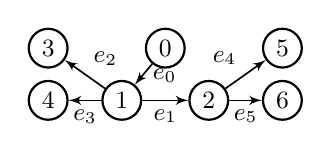
\begin{tikzpicture}[auto, scale=0.85]%, node distance=34mm, thick]
	\small
	\tikzset{mynode/.style={circle,draw,minimum size=14pt,inner sep=0pt,thick},
		myarrow/.style={-, >=latex', shorten >=0pt, line width=0.6pt},
		myarrow_dir/.style={->, >=latex', shorten >=0pt, line width=0.6pt},}
	
	%    \node at (0,-1) {$\bullet$};
	\node[mynode] (n0) at (0.65,0.38) {$0$};
	\node[mynode] (n1) at (0,-0.4) {$1$};
	\node[mynode] (n2) at (1.3,-0.4) {$2$};    
	\node[mynode] (n3) at (-1.1,.38) {$3$};
	\node[mynode] (n4) at (-1.1,-.4) {$4$};
	\node[mynode] (n5) at (2.4,.38) {$5$};
	\node[mynode] (n6) at (2.4,-.4) {$6$};
	
	\path[myarrow_dir] (n1) edge node [yshift=11.5pt, xshift=15pt] {$e_2$} (n3);
	\path[myarrow_dir] (n1) edge node {$e_3$} (n4);
	\path[myarrow_dir] (n1) edge node [yshift=-11.5pt] {$e_1$} (n2);
	\path[myarrow_dir] (n2) edge node {$e_4$} (n5);
	\path[myarrow_dir] (n2) edge node [yshift=-11.5pt, xshift=0pt] {$e_5$} (n6);
	\path[myarrow_dir] (n0) edge node [yshift=5.4pt, xshift=0pt]{$e_0$} (n1);
	
	\end{tikzpicture}
	\vspace{5mm}
	\caption{Interaction topology. \label{fig:topo}}
	\vspace*{-3mm}
	\end{subfigure}
	\hspace*{0.05\textwidth}
	\begin{subfigure}{0.45\textwidth}
		\def\svgwidth{\textwidth}
		\import{figures/handpos_tracking}{formation.pdf_tex}
		\vspace*{-6mm}
		\caption{Desired formation shape. \label{fig:handpos_formation}}
		\vspace*{-3mm}
	\end{subfigure}
	\caption{Illustrations of the simulated example.}
\end{figure}

\subsection{MATLAB Example}
\pgfplotsset{table/search path={figures/handpos_tracking/data}}
\begin{figure}[p]
    \centering
    \begin{subfigure}{0.7\textwidth}
        \centering
        \def\svgwidth{\textwidth}
        \import{figures/handpos_tracking}{sim_trajectory.pdf_tex}
        \vspace*{-6mm}
        \caption{The 3D trajectory of the \glspl{auv}. The black line represents the virtual target.}
        \label{fig:handpos_tracking_trajectory}
    \end{subfigure}  
    \begin{subfigure}{0.47\textwidth}
        \hspace*{-2mm}
        \input{figures/handpos_tracking/sim_formation_errors.tex}
        \vspace*{-6mm}
        \caption{Norms of the formation-keeping errors, $\tilde{\mat{z}}_{1, k}$, and the tracking error, $\tilde{\mat{z}}_{1, o}$.}
        \label{fig:handpos_tracking_formation_errors}
    \end{subfigure}
    \begin{subfigure}{0.47\textwidth}
        \hspace*{1mm}
        \input{figures/handpos_tracking/sim_velocity_errors.tex}
        \vspace*{-6mm}
        \caption{Norms of the velocity errors $\mat{z}_{2, k}$ and $\mat{z}_{2, o}$.}
        \label{fig:handpos_tracking_velocity_errors}
    \end{subfigure}
    \begin{subfigure}{0.47\textwidth}
        \hspace*{-2mm}
        \input{figures/handpos_tracking/sim_distances.tex}
        \vspace*{-6mm}
        \caption{Inter-vehicle distances $\norm{\mat{z}_{1, k}}$. The dashed lines represent the limits $\delta_k$ and $\Delta_k$.}
        \label{fig:handpos_tracking_distances}
    \end{subfigure}
    \begin{subfigure}{0.47\textwidth}
        \vspace*{-40mm}
        \hspace*{1mm}
        \input{figures/handpos_tracking/sim_surge.tex}
        \vspace*{-6mm}
        \caption{Surge velocities of the \glspl{auv}.}
        \label{fig:handpos_tracking_surge}
    \end{subfigure}
    \caption{Results of numerical simulations in MATLAB.}
    \label{fig:handpos_tracking_sim}
\end{figure}


Here we simulate six \acrfullpl{lauv}.
The ocean current velocity is set to $\ocean= \left[0.05\;\;-0.08\;\;-0.03\right]\T$.
The desired formation is illustrated in \figref{fig:handpos_formation}.
The desired relative positions $\mat{z}_{1, k}^d$ are given by
\begin{equation}
	\begin{bmatrix}
		\mat{z}_{1, 1}^d & \cdots & \mat{z}_{1, 5}^d
	\end{bmatrix}
	=
	\begin{bmatrix}
		20 & 10 & 10 & 10 & 10\\ 0 & 15 & -15 & 15 & -15\\ 0 & -5 & -5 & -5 & -5
	\end{bmatrix}
\end{equation}
The trajectory of the virtual target is
\begin{equation}
	\mat{x}_{1, o} = \inlinevector{a \cos(\omega_o t), b \sin(\omega_o t), c \sin(\omega_o t)^2},
\end{equation}
where $a = 60$, $b = 40$, $c = 10$, and $\omega_o = \frac{\pi}{150}$.

The maximal and minimal distance parameters are $\Delta_k=\SI{50}{\meter}$ and $\delta_k=\SI{5}{\meter}$.
The hand position point is chosen at $l=\SI{5}{\meter}$, and the control gains are set to $c_1=0.1$, $c_2=0.5$, $\gamma=0.25$, $c_v=0.2$, $\kappa_u=0.1$, $\kappa_\rho=4$, and $\sigma=0.3$.
Furthermore, in order to avoid discontinuities in the control, the non-smooth ${\rm sign}(s)$ function in \eqref{n338} and \eqref{631} is replaced by the smooth approximation $\tanh\left(c_a\, s\right)$, with $c_a = 10^3$.

\figref{fig:handpos_tracking_sim} presents the results of the simulation scenario.
Specifically, \figref{fig:handpos_tracking_trajectory} shows the 3D trajectories of the \glspl{auv}.
We can see that the vehicles successfully reach the desired formation while following the target, as is also evidenced from the formation and tracking errors in \figref{fig:handpos_tracking_formation_errors} and the velocity errors in \figref{fig:handpos_tracking_velocity_errors}.
Furthermore, note that the hard connectivity and collision-avoidance constraints, shown as dashed black lines in \figref{fig:handpos_tracking_distances}, are always respected.
The soft constraints are satisfied as well, and the surge velocities are kept non-negative, as shown in \figref{fig:handpos_tracking_surge}.
%To see this more clearly, Fig.~\ref{fig:ur} shows the surge velocities for an identical simulation scenario, except for the soft-constraint requirement on the velocities. It is clear by comparing with Fig.~\ref{fig:ur2}, that without the proposed strategy, the surge velocities would take greater negative values.

\subsection{DUNE simulations}
\begin{figure}[p]
    \centering
    \begin{subfigure}{0.7\textwidth}
        \centering
        \def\svgwidth{\textwidth}
        \import{figures/handpos_tracking}{hifi_trajectory.pdf_tex}
        \vspace*{-6mm}
        \caption{The 3D trajectory of the \glspl{auv}. The black line represents the virtual target.}
        \label{fig:handpos_tracking_hifi_trajectory}
    \end{subfigure}  
    \begin{subfigure}{0.47\textwidth}
        \hspace*{-2mm}
        \input{figures/handpos_tracking/hifi_formation_errors.tex}
        \vspace*{-6mm}
        \caption{Norms of the formation-keeping errors, $\tilde{\mat{z}}_{1, k}$, and the tracking error, $\tilde{\mat{z}}_{1, o}$.}
        \label{fig:handpos_tracking_hifi_formation_errors}
    \end{subfigure}
    \begin{subfigure}{0.47\textwidth}
        \hspace*{1mm}
        \input{figures/handpos_tracking/hifi_velocity_errors.tex}
        \vspace*{-6mm}
        \caption{Norms of the velocity errors $\mat{z}_{2, k}$ and $\mat{z}_{2, o}$.}
        \label{fig:handpos_tracking_hifi_velocity_errors}
    \end{subfigure}
    \begin{subfigure}{0.47\textwidth}
        \hspace*{-2mm}
        \input{figures/handpos_tracking/hifi_distances.tex}
        \vspace*{-6mm}
        \caption{Inter-vehicle distances $\norm{\mat{z}_{1, k}}$. The dashed lines represent the limits $\delta_k$ and $\Delta_k$.}
        \label{fig:handpos_tracking_hifi_distances}
    \end{subfigure}
    \begin{subfigure}{0.47\textwidth}
        \vspace*{-40mm}
        \hspace*{-2mm}
        \input{figures/handpos_tracking/hifi_surge.tex}
        \vspace*{-6mm}
        \caption{Surge velocities of the \glspl{auv}.}
        \label{fig:handpos_tracking_hifi_surge}
    \end{subfigure}
    \caption{Results of numerical simulations in \gls{dune}.}
    \label{fig:handpos_tracking_hifi}
\end{figure}


Here, we simulate a formation of six \glspl{lauv} using \gls{dune}.
The parameters of the simulation are chosen identically to the MATLAB example.

\figref{fig:handpos_tracking_hifi} presents the results of the simulation.
Specifically, \figref{fig:handpos_tracking_hifi_trajectory} shows the 3D trajectories of the \glspl{auv}.
We can see that the vehicles manage to reach the desired formation. However, the transient behavior is different from the one under the ideal conditions of the MATLAB simulation.
One reason behind these differences is that in the DUNE simulation, the torque produced by the fins depends on the speed of the vehicle.
Consequently, the \glspl{auv} cannot turn if their speed is too low.
In addition, the surge thrust of the \glspl{auv} is limited.
Consequently, the \glspl{auv} can only reach a surge velocity of $\SI{1.8}{\meter\per\second}$, as shown in \figref{fig:handpos_tracking_hifi_surge}.
Unlike the MATLAB simulations, the soft constraints cannot always be satisfied, and the surge velocities of \glspl{auv} 2 and 5 briefly drop below zero.
Having a negative surge velocity is necessary to satisfy the hard connectivity and collision-avoidance constraints shown as dashed black lines in \figref{fig:handpos_tracking_hifi_distances}.
The formation-tracking errors and the velocity errors are shown in Figures~\ref{fig:handpos_tracking_hifi_formation_errors} and \ref{fig:handpos_tracking_hifi_velocity_errors}, respectively.
We can see that these errros do not converge to zero but rather to a small area around zero.
These nonzero steady-state errors are caused by two factors: the uncertainty of the navigation system, and the delay in the actuators.

\chapter{Combining NSB with the Hand Position Approach}
\label{chap:handpos_NSB}



\chapter{Concluding Remarks and Future Work}
\label{part:conclusions}

\setlength{\epigraphwidth}{0.46\textwidth}
\epigraph{ \it
    We know everything, that is, \\
    that we know nothing.
}{
    L. Smoljak, ``Vyšetřování ztráty třídní knihy,'' 1967 (translated from Czech).
}

In this thesis, we presented and analyzed multiple control algorithms.
The majority of these algorithms solve the formation path-following problem of underactuated \acrfullpl{auv}.
We conclude the thesis by presenting some remarks for each chapter and suggestions for future work.

\subsubsection{Chapter~\ref{chap:collision_avoidance}: \nameref{chap:collision_avoidance}}
In Chapter~\ref{chap:collision_avoidance}, we proposed a method for integrating a \acrfull{colav} scheme into control allocation through the use of \acrfullpl{cbf}.
We demonstrated its effectiveness on two models of \acrfullpl{asv}, where it significantly improved the safety.
The proposed method can be readily implemented on vehicles that already use optimization-based control allocation by simply including the constraints given by the \acrfullpl{cbf} in the optimization.

We note that the performance of the proposed scheme depends on the choice of the parameters, such as the class-$\mathcal{K}_{\infty}$ function $\gamma$, and the weight matrices $\mat{Q}$, $\mat{R}_{\rm abs}$, and $\mat{R}_{\rm rel}$.
Finding a systematic method for choosing the parameter values that guarantee safety for a given vehicle model is a topic for future work.

\subsection*{Part~\ref{part:NSB}: \nameref{part:NSB}}

In this part, we proposed three \gls{nsb} algorithms for solving the formation path-following problem.

\subsubsection{Chapter~\ref{chap:5dof_nsb}: \nameref{chap:5dof_nsb}}

In Chapter~\ref{chap:5dof_nsb}, we proposed a formation path-following method for an arbitrary number of \glspl{auv}, proved the stability of the path following part, and verified its effectiveness in simulations.

Because the proposed algorithm is centralized, our method can only be used in scenarios where all the vehicles can communicate with each other.
A distributed version of the algorithm is introduced later in Chapter~\ref{chap:distr_NSB}.

In the simulations, the formation-keeping error shows exponential convergence to zero.
However, the stability of the formation-keeping task has not been theoretically proven.
A modified version of the algorithm with provable stability of the formation-keeping task is presented in Chapter~\ref{chap:NSB_R}.

\subsubsection{Chapter~\ref{chap:NSB_R}: \nameref{chap:NSB_R}}

This chapter extends the formation path-following \gls{nsb} algorithm to underactuated 6\gls{dof} vehicles while adding obstacle avoidance and depth-limiting capabilities. 
Both the path-following and formation-keeping parts are proven to be stable.     
In the proofs, we assume that the avoidance and depth-limiting tasks are not active.
An analysis of the closed-loop system with active avoidance and depth-limiting tasks is left for future work.

\subsubsection{Chapter~\ref{chap:distr_NSB}: \nameref{chap:distr_NSB}}

In Chapter~\ref{chap:distr_NSB}, we discussed to combine \acrlong{nsb} control with consensus, and in this way solve the formation path-following problem in a fully distributed fashion. We also found that it is possible to implement this concept in two different ways, using a continuous-time consensus algorithm, or a discrete-time one (the latter being more suitable for real-life implementations).
Using Lyapunov analysis, we have shown that in the special case of straight-line paths, the continuous-time version achieves uniform semiglobal exponential stability.
The discrete-time version is based on event-triggered paradigms, so to account for practical limitations in the way agents exchange information.

Both versions are then verified in simulations.
Comparing the discrete-time version to a similar cooperative path following algorithm presented in \cite{praveen_cooperative_2018}, we found 
that the proposed algorithm requires fewer transmissions between the vehicles, while having similar steady-state error.
Finally, we demonstrated the real-life effectiveness of the the discrete-time algorithm in field experiments with a fleet of light autonomous underwater vehicles.

Future work includes extending the stability proofs to the more general case of curved paths and more complex vehicle dynamics, as well as investigating the effects of the event-triggered scheme on the performance of the algorithm.
In addition, we plan to perform additional experiments with more vehicles and underwater communications.

\subsection*{Part~\ref{part:hand_position}: \nameref{part:hand_position}}

In this part, we extended the hand position concept to underactuated \glspl{auv} and presented multiple applications of this concept.

\subsubsection{Chapter~\ref{chap:handpos_definition}: \nameref{chap:handpos_definition}}

In this section, we extended the hand position concept to 6\gls{dof} underactuated underwater vehicles.
By choosing the hand position as the output of our system, we could apply output feedback linearization to simplify the underactuated 6\gls{dof} vehicle dynamics to a double integrator without introducing any singularities.
Then, we introduced the sufficient conditions under which the internal states are ultimately bounded.

As mentioned in the Introduction, the hand position concept and its ability to transform a nonlinear underactuated model to a double integrator without singularities present an opportunity to utilize numerous control strategies that could otherwise not be used on nonholonomic or underactuated vehicles.
Examples of such controllers were presented in Chapters~\ref{chap:handpos_trajectory}--\ref{chap:handpos_NSB}.

\subsubsection{Chapter~\ref{chap:handpos_trajectory}: \nameref{chap:handpos_trajectory}}

In this chapter, we showed how the hand position transformation combined with a simple PID-based controller can be used to solve both the trajectory-tracking and path-following control problems.
Using Lyapunov analysis, we proved the exponential stability of the external dynamics.
Moreover, in the special case of straight-line trajectories and paths, we could modify the controllers and prove the exponential stability of the total system.
The proposed controllers were tested both in numerical simulations and experiments.

\subsubsection{Chapter~\ref{chap:handpos_MPC}: \nameref{chap:handpos_MPC}}

In this chapter, we have proposed a distributed spline-based \gls{mpc} scheme for the formation path-following problem.
We have shown that using splines makes the distributed control problem computationally tractable.
Compared to collocation, the spline parametrization allows us to represent a longer prediction horizon using fewer variables.    
This is also beneficial for the communication, and thus makes it easier to do distributed control in environments where the communication bandwidth is limited (\emph{e.g.,} underwater).

One might argue that restricting the output to splines limits the subspace of feasible trajectories.
However, simulation results show that cubic splines provide a good approximation of many curves.
Another limiting factor is the need for differential flatness.
However, it is often possible to simplify the structure of the model to guarantee differential flatness.        
The proposed spline-based \gls{mpc} scheme can thus be seen as a trade-off between lower computational requirements and more restrictive assumptions on the model.

\subsubsection{Chapter~\ref{chap:handpos_tracking}: \nameref{chap:handpos_tracking}}

In this chapter, we addressed the tracking-in-formation control problem of cooperative autonomous underwater vehicles interacting over directed graphs and under \emph{hard} inter-agent constraints (proximity and collision avoidance) and \emph{soft} constraints (positive surge velocity). 
We proposed a distributed control law that solves this problem and that guarantees, simultaneously, connectivity preservation and inter-agent collision avoidance.
With respect to the stability analysis, it is important to emphasize that, beyond mere convergence properties as usually established in the literature of multi-agent systems, we establish almost-everywhere uniform asymptotic stability with exponential convergence of the tracking errors. 
Current research focuses on validating the results experimentally.

\subsubsection{Chapter~\ref{chap:handpos_NSB}: \nameref{chap:handpos_NSB}}

In this chapter, we proposed an extended \gls{nsb} method for double-integrator systems. The method was proved to provide \acrlongpl{ges} task error dynamics. The method was demonstrated in a case study of formation path-following with underactuated \glspl{auv}. We defined the second-order kinematic tasks for collision avoidance, formation-keeping, and path-following. To force a bounded velocity, we introduced a saturation term to the formation-keeping acceleration. The closed-loop formation-error system with the reformulated formation-keeping acceleration was proved to be \acrlongpl{ugas}, and the closed-loop path-following system was proved to be \acrlongpl{usges}. Simulation results demonstrate the effectiveness of our approach. Possible future work includes verifying the presented results through experiments.


\chapter*{\bibname}
\printbibliography[heading=none]

\appendix
\input{appendices/1-model.tex}
\chapter{Proofs of Lemmas from Chapter \ref{chap:5dof_nsb}}

\section{Derivation of Closed-Loop Barycenter Kinematics}
\label{app:5dof_nsb_barycenter}
We begin by taking $\dot{y}_b^p$ from \eqref{eq:nsb_5dof_y_pb}.
\begin{align}
    \dot{y}_b^p &= \frac{1}{n}\sum_{i=1}^n U_i\,\cos\left(\gamma_i\right)\,\sin\left(\chi_i - \psi_p\right) - \dot{\xi}\,\iota\,x_b^p. \label{eq:nsb_5dof_y_pb_0}
\end{align}
Now, consider the term $\sin\left(\chi_i - \psi_p\right)$.
The course of the vessel is given by
\begin{align}
    \chi_i &= \psi_i + \beta_i, &
    \beta_i &= \arcsin\left(\frac{v_i}{U_i}\right).
\end{align}
After substituting and applying some trigonometric identities, we get
\begin{subequations}
    \begin{align}
        \sin\left(\chi_i - \psi_p\right) &= \sin\left(\psi_i + \beta_i - \psi_p\right) \\
        &= \cos\left(\psi_i - \psi_p\right)\,\sin\left(\beta_i\right) + \sin\left(\psi_i - \psi_p\right)\,\cos\left(\beta_i\right) \\
        &= \cos\left(\psi_i - \psi_p\right)\frac{v_i}{U_i} + \sin\left(\psi_i - \psi_p\right)\frac{\sqrt{u_i^2 + w_i^2}}{U_i}.
    \end{align}
\end{subequations}
Consequently, the term $U_i\,\cos\left(\gamma_i\right)\,\sin\left(\chi_i - \psi_p\right)$ is equivalent to
\begin{equation}
    \begin{split}
        U_i\,\cos\left(\gamma_i\right)\,\sin\left(\chi_i - \psi_p\right) = \cos\left(\gamma_i\right) \bigg(&\cos\left(\psi_i - \psi_p\right)v_i \\
        & \quad + \sin\left(\psi_i - \psi_p\right)\sqrt{u_i^2 + w_i^2}\bigg). 
    \end{split}
    \label{eq:nsb_5dof_y_pb_1}
\end{equation}

\noindent Now, consider a term $\sin\left(\psi_i + \beta_{d,i} - \psi_p\right)$.
Using a similar procedure, we get
\begin{equation}
    \sin\left(\psi_i + \beta_{d,i} - \psi_p\right) = \cos\left(\psi_i - \psi_p\right)\frac{v_i}{U_{d,i}} + \sin\left(\psi_i - \psi_p\right)\frac{\sqrt{u_{d,i}^2 + w_i^2}}{U_{d,i}}. \label{eq:nsb_5dof_y_pb_2}
\end{equation}
Combining \eqref{eq:nsb_5dof_y_pb_1} and \eqref{eq:nsb_5dof_y_pb_2}, we get
\begin{equation}
    \begin{split}
    U_i\,\cos\left(\gamma_i\right)\,\sin\left(\chi_i - \psi_p\right) &= U_{d,i}\,\cos\left(\gamma_i\right)\,\sin\left(\psi_i + \beta_{d,i} - \psi_p\right) \\
    &\, +\! \cos\left(\gamma_i\right)\sin\left(\psi_{i\!} - \psi_p\right) \! \left(\!\sqrt{u_i^2\! + \!w_i^2} -\! \sqrt{u_{d,i}^2\! + w_i^2}\right). 
    \end{split}
    \label{eq:nsb_5dof_y_pb_3}
\end{equation}
Note that the following holds for the angles
\begin{equation}
    \begin{split}
        \psi_i + \beta_{d,i} - \psi_p &= \psi_{d,i} + \tilde{\psi}_i + \beta_{d,i} - \left(\psi_{d,i} + \beta_{d,i} + \beta_{\rm LOS}\right) = \tilde{\psi}_i - \beta_{\rm LOS}, \\
        \beta_{\rm LOS} &= \scale[1]{\arctan\left(\frac{y_b^p}{\Delta\left(\mat{p}_b^p\right)}\right)}.
    \end{split}
\end{equation}
Therefore, their sine is given by
\begin{equation}
    \sin\left(\psi_i + \beta_{d,i} - \psi_p\right) = \sin\left(\tilde{\psi}_i\right)\,\scale[1]{\frac{\Delta\left(\mat{p}_b^p\right)}{\sqrt{\Delta\left(\mat{p}_b^p\right)^2 + \left(y_b^p\right)^2}}} - \cos\left(\tilde{\psi}_i\right)\scale[1]{\frac{y_b^p}{\sqrt{\Delta\left(\mat{p}_b^p\right)^2 + \left(y_b^p\right)^2}}}.
    \label{eq:nsb_5dof_sin_psi_beta}
\end{equation}
Furthermore, note that the following holds for the flight-path angle
\begin{equation}
    \gamma_i = \theta_i - \alpha_i = \tilde{\theta}_i + \theta_{d,i} - \alpha_i = \tilde{\theta}_i + \gamma_{\rm LOS} + \alpha_{d,i} - \alpha_i.
\end{equation}
Consequently, the cosine of the flight-path angle is equal to
\begin{equation}
    \begin{split}
    \cos\left(\gamma_i\right) &= \cos\left(\gamma_{\rm LOS}\right)\cos\left(\tilde{\theta}_i\right)\cos\left(\alpha_{d,i} - \alpha_i\right) \\
        &\quad - \cos\left(\gamma_{\rm LOS}\right)\sin\left(\tilde{\theta}_i\right)\sin\left(\alpha_{d,i} - \alpha_i\right) \\
        & \quad - \sin\left(\gamma_{\rm LOS}\right)\cos\left(\tilde{\theta}_i\right)\sin\left(\alpha_{d,i} - \alpha_i\right) \\
        & \quad - \sin\left(\gamma_{\rm LOS}\right)\sin\left(\tilde{\theta}_i\right)\cos\left(\alpha_{d,i} - \alpha_i\right)
    \end{split}
    \label{eq:nsb_5dof_cos_gamma_i}
\end{equation}
Using the equalities \eqref{eq:nsb_5dof_sin_psi_beta}, \eqref{eq:nsb_5dof_cos_gamma_i}, we can rewrite \eqref{eq:nsb_5dof_y_pb_3} as
\begin{equation}
    \begin{split}
        U_i\,\cos\left(\gamma_i\right)\,\sin\left(\chi_i - \psi_p\right) &= - U_{d,i}\cos\left(\gamma_{\rm LOS}\right)\scale[1]{\frac{y_b^p}{\sqrt{\Delta\left(\mat{p}_b^p\right)^2 + \left(y_b^p\right)^2}}} \\
        & \quad + G_{y,i}\left(\tilde{u}_i, \tilde{\psi}_i, \gamma_i, u_{d,i}, v_i, w_i, \mat{p}_b^p, \psi_p\right),
    \end{split}
    \label{eq:nsb_5dof_y_pb_4}
\end{equation}
where
\begin{equation}
    \begin{split}
        G_{y,i}(\cdot) &= \cos\left(\gamma_i\right)\,\sin\left(\psi_i - \psi_p\right)\left(\sqrt{u_i^2 + w_i^2} - \sqrt{u_{d,i}^2 + w_i^2}\right) \\
        &\quad - U_{d,i}\cos\left(\gamma_i\right)\,\sin\left(\tilde{\psi}_i\right)\scale[1]{\frac{\Delta\left(\mat{p}_b^p\right)}{\sqrt{\Delta\left(\mat{p}_b^p\right)^2 + \left(y_b^p\right)^2}}} \\
        &\quad + U_{d,i}\bigg[\sin\!\left(\gamma_{\rm LOS}\right)\!\left(\cos\!\left(\tilde{\theta}_i\right)\!\sin\!\left(\alpha_{d,i} - \alpha_i\right) + \sin\!\left(\tilde{\theta}_i\right)\!\cos\!\left(\alpha_{d,i} - \alpha_i\right)\right) \\
        & \qquad \qquad -\cos\left(\gamma_{\rm LOS}\right)\left(\cos\left(\tilde{\theta}_i\right)\cos\left(\alpha_{d,i} - \alpha_i\right) - 1\right)\bigg]\scale[1]{\frac{y_b^p}{\sqrt{\Delta\left(\mat{p}_b^p\right)^2 + \left(y_b^p\right)^2}}} 
    \end{split} \label{eq:nsb_5dof_G_y}
\end{equation}

\noindent Substituting \eqref{eq:nsb_5dof_y_pb_4} into \eqref{eq:nsb_5dof_y_pb_0}, we get the following
\begin{equation}
    \begin{split}
        \dot{y}_b^p &= - \frac{1}{n}\sum_{i=1}^n U_{d,i}\cos\left(\gamma_{\rm LOS}\right)\scale[1]{\frac{y_b^p}{\sqrt{\Delta\left(\mat{p}_b^p\right)^2 + \left(y_b^p\right)^2}}} - \dot{\xi}\,\iota\,x_b^p \\
        &\quad + G_y\bigg(\tilde{u}_1, \ldots, \tilde{u}_n, \tilde{\psi}_1, \ldots, \tilde{\psi}_n, \gamma_1, \ldots, \gamma_n, u_{d,1}, \ldots, u_{d,n}, \\
        & \qquad \qquad \quad v_1, \ldots, v_n, w_1, \ldots, w_n, \mat{p}_b^p, \psi_p\bigg),
    \end{split}
\end{equation}
where
\begin{equation}
    G_y(\cdot) = \frac{1}{n} \sum_{i=1}^n G_{y,i}\left(\tilde{u}_i, \tilde{\psi}_i, \gamma_i, u_{d,i}, v_i, w_i, \mat{p}_b^p, \psi_p\right).
\end{equation}

Now, we demonstrate a similar procedure for $\dot{z}_b^p$.
From \eqref{eq:nsb_5dof_y_pb}, we get
\begin{equation}
    \begin{split}
        \dot{z}_b^p &= \frac{1}{n} \sum_{i=1}^n U_i \left(-\cos\left(\theta_p\right)\sin\left(\gamma_i\right) + \cos\left(\gamma_i\right)\sin(\theta_p)\cos\left(\psi_p-\chi_i\right)\right) + \dot{\xi}\,\kappa\,x_b^p \\
        &= \frac{1}{n} \sum_{i=1}^n U_i \left(-\sin\left(\gamma_i - \theta_p\right) - \left(1 - \cos\left(\chi_i - \psi_p\right)\right)\cos\left(\gamma_i\right)\sin(\theta_p)\right) + \dot{\xi}\,\kappa\,x_b^p. 
    \end{split} \label{eq:nsb_5dof_z_pb_1}
\end{equation}
Once again, we consider the terms
\begin{equation}
    \sin\left(\gamma_i - \theta_p\right) = \sin\left(\theta_i - \alpha_i - \theta_p\right) = \sin\left(\theta_i - \theta_p\right)\frac{u_i}{U_i} - \cos\left(\theta_i - \theta_p\right)\frac{w_i}{U_i},
\end{equation}
and
\begin{equation}
    \sin\left(\theta_i - \alpha_{d,i} - \theta_p\right) = \sin\left(\theta_i - \theta_p\right)\frac{u_{d,i}}{U_{d,i}} - \cos\left(\theta_i - \theta_p\right)\frac{w_i}{U_{d,i}},
\end{equation}
which give us the following equality
\begin{equation}
    U_i\,\sin\left(\gamma_i - \theta_p\right) = U_{d,i}\,\sin\left(\theta_i - \alpha_{d,i} - \theta_p\right) + \tilde{u}_i\,\sin\left(\theta_i - \theta_p\right).
\end{equation}
Using a similar trick, we can write the sine as
\begin{equation}
    \sin\left(\theta_i - \alpha_{d,i} - \theta_p\right) = \sin\!\left(\tilde{\theta}_i\right)\!\frac{\Delta\!\left(\mat{p}_b^p\right)}{\sqrt{\Delta\!\left(\mat{p}_b^p\right)^2\! +\! \left(z_b^p\right)^2}} -\, \cos\!\left(\tilde{\theta}_i\right)\!\frac{\left(z_b^p\right)}{\sqrt{\Delta\!\left(\mat{p}_b^p\right)^2 \!+\! \left(z_b^p\right)^2}}
\end{equation}
Consequently, we can rewrite \eqref{eq:nsb_5dof_z_pb_1} as
\begin{equation}
    \begin{split}
        \dot{z}_b^p &= - \frac{1}{n} \sum_{i=1}^n U_{d,i}\frac{z_b^p}{\sqrt{\Delta\left(\mat{p}_b^p\right)^2 + \left(z_b^p\right)^2}} + \dot{\xi}\,\kappa\,x_b^p \\
        & \quad + G_z\bigg(\tilde{u}_1, \ldots, \tilde{u}_n, \tilde{\theta}_1, \ldots, \tilde{\theta}_n, \gamma_1, \ldots, \gamma_n, \chi_1, \ldots, \chi_n, \\
        & \qquad \qquad \quad u_{d,1}, \ldots, u_{d,n}, v_1, \ldots, v_n, w_1, \ldots, w_n, \mat{p}_b^p, \theta_p, \psi_p\bigg),
    \end{split}
\end{equation}
where
\begin{align}
    G_z(\cdot) &= \frac{1}{n} \sum_{i=1}^n G_{z,i}\left(\tilde{u}_i, \tilde{\theta}_i, \gamma_i, \chi_i, u_{d,i}, v_i, w_i, \mat{p}_b^p, \theta_p, \psi_p\right), \\
    \begin{split}
        G_{z,i}(\cdot) &= -U_i\left(\left(1 - \cos\left(\chi_i - \psi_p\right)\right)\cos\left(\gamma_i\right)\sin(\theta_p)\right) - \tilde{u}_i\,\sin\left(\theta_i - \theta_p\right) \\
        & \quad -\! \left(1 - \cos\!\left(\tilde{\theta}_{i\!}\right)\right)\!\frac{\left(z_b^p\right)}{\sqrt{\Delta\!\left(\mat{p}_b^p\right)^2\! +\! \left(z_b^p\right)^2}} - U_{d,i}\sin\!\left(\tilde{\theta}_i\right)\!\frac{\Delta\!\left(\mat{p}_b^p\right)}{\sqrt{\Delta\!\left(\mat{p}_b^p\right)^2\! +\! \left(z_b^p\right)^2}}.
    \end{split} \label{eq:nsb_5dof_G_z}
\end{align}

\section{Desired Pitch and Yaw Rate}
For further calculations, we need to evaluate the desired pitch ($q_{d,i}$) and yaw ($r_{d,i}$) rates of the vessels.
From \eqref{eq:nsb_5dof_theta_dot}, we get the following relation between the yaw rate and the derivative of the yaw angle
\begin{equation}
    q_{d,i} = \dot{\theta}_{d,i}.
\end{equation}
Now, we consider the desired pitch angle from \eqref{eq:nsb_5dof_theta_d}.
Since we are investigating the path following task, we substitute $\gamma_{\rm LOS}$ from \eqref{eq:nsb_5dof_v_LOS} for $\gamma_{{\rm NSB}, i}$.
Differentiating \eqref{eq:nsb_5dof_theta_d} with respect to time yields
\begin{equation}
    q_{d,i} = \dot{\theta}_p(\xi) + \frac{\Delta\left(\mat{p}_b^p\right)\,\dot{z}_b^p - z_b^p\,\dot{\Delta}\left(\mat{p}_b^p\right)}{\Delta\left(\mat{p}_b^p\right)^2 + \left(z_b^p\right)^2} + \frac{u_{d,i}\,\dot{w}}{u_{d,i}^2 + w_i^2},
\end{equation}
which can be expanded to
\begin{equation}
    \begin{split}
        q_{d,i} &= \dot{\xi}\,\kappa(\xi) + \frac{\Delta\left(\mat{p}_b^p\right)\left(\frac{1}{n} \sum\limits_{j=1}^n U_{d,j}\frac{\left(z_b^p\right)}{\sqrt{\Delta\left(\mat{p}_b^p\right)^2 + \left(z_b^p\right)^2}} + \dot{\xi}\,\kappa\,x_b^p + G_z(\cdot)\right)}{\Delta\left(\mat{p}_b^p\right)^2 + \left(z_b^p\right)^2} \\
        &\quad + \frac{z_b^p\!\left(\!-k_{\xi}\frac{\left(x_b^p\right)^2}{\sqrt{1+\left(x_b^p\right)^2}} - \frac{1}{n}\!\sum\limits_{j=1}^n \!U_{d,j}\!\left(\!\scale[1]{\frac{\cos\left(\gamma_{{\rm LOS},j}\right)^2\left(y_b^p\right)^2}{\sqrt{\Delta\left(\mat{p}_b^p\right)^2 + \left(y_b^p\right)^2}}}\! + \!\frac{\left(z_b^p\right)^2}{\sqrt{\Delta\left(\mat{p}_b^p\right)^2 + \left(z_b^p\right)^2}}\!\right)\right)}{\Delta\left(\mat{p}_b^p\right)\left(\Delta\left(\mat{p}_b^p\right)^2 + \left(z_b^p\right)^2\right)} \\
        &\quad + \frac{z_b^p\!\left(y_b^p\,G_y(\cdot) \!+\! z_b^p\,G_z(\cdot)\right)}{\Delta\!\left(\mat{p}_b^p\right)\!\left(\Delta\!\left(\mat{p}_b^p\right)^2 \!+\! \left(z_b^p\right)^2\right)} \\
        & \quad + u_{d,i}\frac{X_w\!\left(u_{d,i}+\tilde{u}_i, u_c\right)\!q + Y_w\!\left(u_{d,i}+\tilde{u}_i, u_c\right)\!\left(w_i - w_c\right)}{u_{d,i}^2 + w_i^2}.
    \end{split}
    \label{eq:nsb_5dof_q_d}
\end{equation}

From \eqref{eq:nsb_5dof_psi_dot}, we get the following relation between the yaw rate and the derivative of the yaw angle
\begin{equation}
    r_{d,i} = \dot{\psi}_{d,i}\,\cos\left(\theta_{d,i}\right).
\end{equation}
Substituting the time-derivative of \eqref{eq:nsb_5dof_psi_d}, we get
\begin{subequations}
    \begin{align}
        r_{d,i} &= \left(\dot{\psi}_p(\xi) - \frac{\Delta\!\left(\mat{p}_b^p\right)\,\dot{y}_b^p - y_b^p\,\dot{\Delta}\left(\mat{p}_b^p\right)}{\Delta\!\left(\mat{p}_b^p\right)^2 + \left(y_b^p\right)^2} - \frac{\dot{v}}{\sqrt{U_{d,i}^2 - v_i^2}}\right)\,\cos\left(\theta_{d,i}\right) \\
        \begin{split}
            &= \left[\dot{\xi}\,\iota(\xi) - \frac{\Delta\!\left(\mat{p}_b^p\right)\left(\frac{1}{n} \sum\limits_{j=1}^n U_{d,i}\frac{\cos\left(\gamma_{\rm LOS}\right)\left(y_b^p\right)}{\sqrt{\Delta\!\left(\mat{p}_b^p\right)^2 + \left(y_b^p\right)^2}} - \dot{\xi}\,\iota\,x_b^p + G_y(\cdot)\right)}{\Delta\!\left(\mat{p}_b^p\right)^2 + \left(y_b^p\right)^2} \right. \\
            &\qquad + \frac{y_b^p\!\left(\!-k_{\xi}\frac{\left(x_b^p\right)^2}{\sqrt{1+\left(x_b^p\right)^2}} - \frac{1}{n}\!\sum\limits_{j=1}^n\! U_{d,i}\!\!\left(\!\scale[1]{\frac{\cos\left(\gamma_{\rm LOS}\right)^2\left(y_b^p\right)^2}{\sqrt{\Delta\left(\mat{p}_b^p\right)^2 + \left(y_b^p\right)^2}}} +\! \frac{\left(z_b^p\right)^2}{\sqrt{\Delta\!\left(\mat{p}_b^p\right)^2\! + \left(z_b^p\right)^2}}\right)\!\right)}{\Delta\!\left(\mat{p}_b^p\right)\left(\Delta\!\left(\mat{p}_b^p\right)^2 + \left(y_b^p\right)^2\right)} \\
            &\qquad + \frac{y_b^p \left(y_b^p\,G_y(\cdot) + z_b^p\,G_z(\cdot)\right)}{\Delta\!\left(\mat{p}_b^p\right)\left(\Delta\!\left(\mat{p}_b^p\right)^2 + \left(y_b^p\right)^2\right)} \\
            &\qquad \left. -\frac{X\left(u_{d,i}+\tilde{u}_i, u_c\right)\,r + Y\left(u_{d,i}+\tilde{u}_i, u_c\right)\left(v_i - v_c\right)}{\sqrt{u_{d,i}^2 + w_i^2}} \right]\, \cos\left(\theta_{d,i}\right).
        \end{split}
    \end{align} \label{eq:nsb_5dof_r_d}
\end{subequations}

\section{Proof of Lemma \ref{lemma_1}}
\label{app:5dof_nsb_lemma_1}
In \cite{moe_LOS_2016}, it is shown that the error states \eqref{eq:nsb_5dof_u_tilde}--\eqref{eq:nsb_5dof_psi_tilde} are UGES and the ocean current estimate errors \eqref{eq:nsb_5dof_V_c_tilde}--\eqref{eq:nsb_5dof_theta_r_tilde} are bounded, which implies that \eqref{eq:nsb_5dof_u_tilde}--\eqref{eq:nsb_5dof_theta_r_tilde} are forward complete.
Therefore, we only need to prove that the underactuated sway and heave dynamics \eqref{eq:nsb_5dof_v_dot}, \eqref{eq:nsb_5dof_w_dot} and the barycenter dynamics \eqref{eq:nsb_5dof_x_pb_CL}--\eqref{eq:nsb_5dof_z_pb_CL} are forward complete.

First, let us consider the underactuated sway dynamics.
From \eqref{eq:nsb_5dof_v_dot}, we get
\begin{equation}
    \dot{v}_i = X_v\left(\tilde{u}_i + u_{d,i}, u_c\right)\,\left(\tilde{r}_i + r_{d,i}\right) + Y_v\left(\tilde{u}_i + u_{d,i}, u_c\right)\,\left(v_i - v_c\right),
\end{equation}
where $\tilde{r}_i = r_i - r_{d,i}$.
Now, let us consider a Lyapunov function candidate
\begin{equation}
    V_v(v_i) = \frac{1}{2} v_i^2. \label{eq:nsb_5dof_V_v}
\end{equation}
Its derivative along the trajectories of $v_i$ is
\begin{equation}
    \dot{V}_v(v_i) = X_v\!\left(\tilde{u}_i + u_{d,i}, u_c\right)\left(\tilde{r}_i + r_{d,i}\right)v_i + Y_v\!\left(\tilde{u}_i + u_{d,i}, u_c\right)\left(v_i - v_c\right)v_i. \label{eq:nsb_5dof_V_v_dot}
\end{equation}
From the boudedness of $\tilde{\mat{X}}_{2,i}$, $\kappa(\xi)$, $\iota(\xi)$, $u_{d,i}$, $u_c$ and $v_c$, we can conclude that there exists some scalar $\beta_{v,0} > 0$ such that
\begin{equation}
    \left\| \left[ \tilde{\mat{X}}_{2,i}\T, \kappa(\xi), \iota(\xi), u_{d,i}, u_c, v_c \right]\T \right\| \leq \beta_0.
\end{equation}
Moreover, from \eqref{eq:nsb_5dof_r_d}, we can conclude that there exist some positive functions $a_r(\beta_{v,0})$ and $b_r(\beta_{v,0})$ such that
\begin{equation}
    \abs{r_{d,i}} \leq a_r(\beta_{v,0})\,\abs{v_i} + b_r(\beta_{v,0}).
\end{equation}
Consequently, we can upper bound $\dot{V}_v(v_i)$ using the following expression
\begin{equation}
    \begin{split}
        \dot{V}_v(v_i) &\leq X_v\left(\tilde{u}_i + u_{d,i}, u_c\right)\left(\tilde{r}_i\,v_i + a_r(\cdot)v_i^2 + b_r(\cdot)v_i\right) \\
        &\quad + Y_v\left(\tilde{u}_i + u_{d,i}, u_c\right)\left(v_i^2 - v_c\,v_i\right).
    \end{split}
\end{equation}
Using Young's inequality, we get
\begin{subequations}
    \begin{align}
        \begin{split}
            \dot{V}_v(v_i) &\leq \left(X_v\left(\tilde{u}_i + u_{d,i}, u_c\right)\left(2 + a_r(\cdot)\right) + 2\,Y_v\left(\tilde{u}_i + u_{d,i}, u_c\right)\right)\,v_i^2 \\
             & \quad + X_v\left(\tilde{u}_i + u_{d,i}, u_c\right)\left(\tilde{r}_i^2 + b_r(\cdot)^2\right) + Y_v\left(\tilde{u}_i + u_{d,i}, u_c\right)\,v_c^2
        \end{split} \\
        & \leq \alpha_v\,V_v(v_i) + \beta_v.
    \end{align}
\end{subequations}
Using the comparison lemma, we get
\begin{equation}
    V_v\left(v_i(t)\right) \leq \left(V_v\left(v_i(t_0)\right) + \frac{\beta_v}{\alpha_v}\right)\,{\rm exp}\left(\alpha_v(t - t_0)\right) - \frac{\beta_v}{\alpha_v}.
\end{equation}
As $V_v(v_i)$ is defined for all $t > t_0$, it follows that $v_i$ is also defined for all $t > t_0$.
The solutions of \eqref{eq:nsb_5dof_v_dot} thus fulfill the definition of forward completeness, as defined in \cite{angeli_forward_1999}.

Now, let us consider the underactuated heave dynamics.
From \eqref{eq:nsb_5dof_w_dot}, we get
\begin{equation}
    \dot{w}_i = X_w\!\left(\tilde{u}_i + u_{d,i}, u_c\right)\left(\tilde{q}_i + q_{d,i}\right) + Y_w\!\left(\tilde{u}_i + u_{d,i}, u_c\right)\left(w_i - w_c\right) + G(\theta_i),
\end{equation}
where $\tilde{q}_i = q_i - q_{d,i}$.
Similar to the previous paragraph, we consider a Lyapunov function candidate
\begin{equation}
    V_w(w_i) = \frac{1}{2} w_i^2, \label{eq:nsb_5dof_V_w}
\end{equation}
whose derivative is
\begin{equation}
    \begin{split}
        \dot{V}_w(w_i) &= X_w\left(\tilde{u}_i + u_{d,i}, u_c\right)\,\left(\tilde{q}_i + q_{d,i}\right)\,w_i \\
        &\quad + Y_w\left(\tilde{u}_i + u_{d,i}, u_c\right)\,\left(w_i - w_c\right)\,w_i + G(\theta)\,w_i.
    \end{split}
\end{equation}
From the boudedness of $\tilde{\mat{X}}_{2,i}$, $\kappa(\xi)$, $\iota(\xi)$, $u_{d,i}$, $u_c$ and $w_c$, we can conclude that there exists some scalar $\beta_0 > 0$ such that 
\begin{equation}
    \left\| \left[ \tilde{\mat{X}}_{2,i}\T, \kappa(\xi), \iota(\xi), u_{d,i}, u_c, w_c \right]\T \right\| \leq \beta_{w,0}.
\end{equation}
Moreover, from \eqref{eq:nsb_5dof_q_d}, we can conclude that there exist some positive functions $a_q(\beta_{w,0})$ and $b_q(\beta_{w,0})$ such that
\begin{equation}
    \abs{q_{d,i}} \leq a_q(\beta_{w,0})\,\abs{w_i} + b_q(\beta_{w,0}).
\end{equation}
Consequently, we can upper bound $\dot{V}_w(w_i)$ using the following expression
\begin{equation}
    \begin{split}
        \dot{V}_w(w_i) &\leq X_w\left(\tilde{u}_i + u_{d,i}, u_c\right)\left(\tilde{q}_i\,w_i + a_q(\cdot)w_i^2 + b_q(\cdot)w_i\right) \\
        &\quad + Y_w\left(\tilde{u}_i + u_{d,i}, u_c\right)\left(w_i^2 - w_c\,w_i\right) + G(\theta_i)\,w_i.
    \end{split}
\end{equation}
Using Young's inequality, we get
\begin{equation}
    \begin{split}
        \dot{V}_w(w_i) &\leq \left(X_w\left(\tilde{u}_i + u_{d,i}, u_c\right)\left(2 + a_q(\cdot)\right) + 2\,Y_w\left(\tilde{u}_i + u_{d,i}, u_c\right) + 1\right)\,w_i^2 \\
        & \quad + X_w\left(\tilde{u}_i + u_{d,i}, u_c\right)\left(\tilde{q}_i^2 + b_q(\cdot)^2\right) + Y_w\left(\tilde{u}_i + u_{d,i}, u_c\right)\,w_c^2 + G(\theta)^2 \\
        & \leq \alpha_w\,V_w(w_i) + \beta_w.
    \end{split}
\end{equation}
Using the comparison lemma, we get
\begin{equation}
    V_w\left(w_i(t)\right) \leq \left(V_w\left(w_i(t_0)\right) + \frac{\beta_w}{\alpha_w}\right)\,{\rm exp}\left(\alpha_w(t - t_0)\right) - \frac{\beta_w}{\alpha_w}.
\end{equation}
Using the same arguments as in the previous paragraph, we conclude that the solutions of \eqref{eq:nsb_5dof_w_dot} are forward complete.

Finally, let us consider the barycenter dynamics.
We use a Lyapunov function candidate
\begin{equation}
    V_b(\mat{p}_b^p) = \frac{1}{2} \left(\left(x_b^p\right)^2 + \left(y_b^p\right)^2 + \left(z_b^p\right)^2\right),
\end{equation}
whose derivative along the solutions of \eqref{eq:nsb_5dof_x_pb_CL}--\eqref{eq:nsb_5dof_z_pb_CL} is
\begin{equation}
    \begin{split}
        \dot{V}_b\left(\mat{p}_b^p\right) &= -k_{\xi}\frac{\left(x_b^p\right)^2}{\sqrt{1 + \left(x_b^p\right)^2}} + G_y(\cdot)\,y_b^p + G_z(\cdot)\,z_b^p \\
        &\quad - \frac{1}{n}\sum_{i=1}^n U_{d,i} \left(
            \frac{\cos\left(\gamma_{\rm LOS}\right)^2\left(y_b^p\right)^2}{\sqrt{\Delta\left(\mat{p}_b^p\right)^2 + \left(y_b^p\right)^2}} +
            \frac{\left(z_b^p\right)^2}{\sqrt{\Delta\left(\mat{p}_b^p\right)^2 + \left(z_b^p\right)^2}}
        \right) \\
        &\leq G_y(\cdot)\,y_b^p + G_z(\cdot)\,z_b^p + \frac{1}{2} \left(x_b^p\right)^2.
    \end{split}
\end{equation}
Using Young's inequality, we get
\begin{equation}
    \begin{split}
        \dot{V}_b\left(\mat{p}_b^p\right) &\leq \frac{1}{2} \left(\left(x_b^p\right)^2 + \left(y_b^p\right)^2 + \left(z_b^p\right)^2\right) + \frac{1}{2}\left(G_y(\cdot)^2 + G_z(\cdot)^2\right) \\
        &\leq V_b\left(\mat{p}_b^p\right) + \frac{1}{2}\left(G_y(\cdot)^2 + G_z(\cdot)^2\right).
    \end{split}
\end{equation}
Note that from \eqref{eq:nsb_5dof_G_y} and \eqref{eq:nsb_5dof_G_z}, we can conclude that there exist some positive function $\zeta_y(U_{d,1}, \ldots, U_{d,n})$ and $\zeta_z(U_{d,1}, \ldots, U_{d,n})$ such that
\begin{align}
    \abs{G_y(\cdot)} \leq \zeta_y(\cdot) \left\| \left[\tilde{u}_1, \ldots, \tilde{u}_n, \tilde{\psi}_1, \ldots, \tilde{\psi}_n\right]\T \right\|, \\
    \abs{G_z(\cdot)} \leq \zeta_z(\cdot) \left\| \left[\tilde{u}_1, \ldots, \tilde{u}_n, \tilde{\theta}_1, \ldots, \tilde{\theta}_n\right]\T \right\|.
\end{align}
Consequently, there exists a class-$\mathcal{K}_{\infty}$ function $\zeta_p(\cdot)$ such that
\begin{equation}
    \begin{split}
        \dot{V}_p\left(\mat{p}_b^p\right) \leq V_p\left(\mat{p}_b^p\right) + \zeta_p\bigg(&v_1, \ldots, v_n, w_1, \ldots, w_n, \tilde{u}_1, \ldots, \tilde{u}_n, \\
        &\quad \tilde{\psi}_1, \ldots, \tilde{\psi}_n, \tilde{\theta}_1, \ldots, \tilde{\theta}_n\bigg).
    \end{split}
\end{equation}
Since all the arguments of $\zeta_p(\cdot)$ are forward complete, Corollary 2.11 of \cite{angeli_forward_1999} is satisfied and the barycenter dynamics is forward complete, thus concluding the proof of Lemma~\ref{lemma_1}.

\section{Proof of Lemma \ref{lemma_2}}
\label{app:5dof_nsb_lemma_2}
First, we consider the sway dynamics.
We take the Lyapunov function candidate $V_v$ from \eqref{eq:nsb_5dof_V_v} and simplify its derivative by setting $\left[\tilde{\mat{X}}_1\T, \tilde{\mat{X}}_2\T\right] = \mat{0}\T$.
\begin{equation}
    \dot{V}_v(v_i) = X_v\left(u_{d,i}, u_c\right)\,r_{d,i}\,v_i + Y_v\left(u_{d,i}, u_c\right)\,\left(v_i - v_c\right)\,v_i. \label{eq:nsb_5dof_V_v_dot_2}
\end{equation}
Next, we find an upper bound on $r_{d,i}\,v_i$.
We substitute from \eqref{eq:nsb_5dof_r_d}, set $\left[\tilde{\mat{X}}_1\T, \tilde{\mat{X}}_2\T\right] = \mat{0}\T$ and collect all terms that grow linearly with $v_i$ to obtain the following expression
\begin{align}
    \scale[0.95]{r_{d,i}\,v_i}\, &\scale[0.95]{= \!\left(\! v_i\!\left(\!1 \!+\! \frac{\Delta(\mat{p}_b^p)\,x_b^p}{\Delta(\mat{p}_b^p)^2 + \left(x_b^p\right)^2}\!\right)\! \iota(s) \frac{1}{n}\!\! \sum\limits_{j=1}^n \!U_j\Omega_x(\gamma_j, \theta_p, \chi_j, \psi_p) \!+\! \frac{Y_v(u_{d,i}, u_c)}{\sqrt{u_{d,i}^2 + w_i^2}}v_i^{2\!}\! \right)\! \cos(\theta_{d,i})} \nonumber \\
    &\quad \scale[0.95]{+ F_v(u_{d,i}, u_c, v_c, v_i, w_i, r_i, \theta_{d, i}),}
\end{align}
where
\begin{equation}
    \scale[1]{F_v(\cdot) = \frac{X_v(u_{d,i}, u_c)\,r_i - Y_v(u_{d,i}, u_c)\,v_c}{\sqrt{u_{d,i}^2 + w_i^2}} v_i \, \cos(\theta_{d,i}).}
\end{equation}
We can bound this expression as
\begin{align}
    \abs{r_{d,i}\,v_i} &\leq \frac{2}{n}\abs{v_i}\,\abs{\iota(\xi)}\sum_{j=1}^n\left(\abs{u_j} + \abs{v_j} + \abs{w_j}\right) + \abs{F_v(\cdot)} \nonumber \\
    &\leq \frac{2}{n}\abs{\iota(\xi)}\,v_i^2 + \frac{2}{n}\abs{v_i}\,\abs{\iota(\xi)}\left(\sum_{j \neq i}\bigl(\abs{u_j} + \abs{v_j} + \abs{w_j}\bigr) + \abs{u_i} + \abs{w_i}\right) \nonumber \\
    &\quad + \abs{F_v(u_{d,i}, u_c, v_c, v_i, w_i, r_i, \theta_{d, i})},
\end{align}
which we can substitute to \eqref{eq:nsb_5dof_V_v_dot_2} to obtain
\begin{equation}
    \begin{split}
        \dot{V}_v(v_i) &\leq \left(X_v\left(u_{d,i}, u_c\right)\frac{2}{n}\abs{\iota(\xi)} + Y_v\left(u_{d,i}, u_c\right)\right)v_i^2 \\
        &\quad + \left(\frac{2}{n}\abs{v_i}\,\abs{\iota(\xi)}\sum_{j \neq i}\bigl(\abs{u_j} + \abs{v_j} + \abs{w_j}\bigr) + \abs{u_i} + \abs{w_i}\right) \\
        & \quad + \left(\abs{F_v(\cdot)} - Y_v\left(u_{d,i}, u_c\right)\abs{v_c}\right) \abs{v_i}.
    \end{split}
\end{equation}
For a sufficiently large $v_i$, the quadratic term will dominate the linear term.
Therefore, we can conclude that $v_i$ is bounded if 
\begin{equation}
    X_v\left(u_{d,i}, u_c\right)\frac{2}{n}\abs{\iota(\xi)} + Y_v\left(u_{d,i}, u_c\right) < 0.
\end{equation}
Since $Y_v$ is assumed to be always negative, the inequality is satisfied if
\begin{equation}
    \abs{\iota(\xi)} < \frac{n}{2}\abs{\frac{Y_v\left(u_{d,i}, u_c\right)}{X_v\left(u_{d,i}, u_c\right)}}.
\end{equation}

Now, we perform a similar procedure for the heave dynamics.
We take the Lyapunov function candidate $V_w$ from \eqref{eq:nsb_5dof_V_w} and simplify its derivative by setting $\left[\tilde{\mat{X}}_1\T, \tilde{\mat{X}}_2\T\right] = \mat{0}\T$.
\begin{equation}
    \dot{V}_w(w_i) = X_w\left(u_{d,i}, u_c\right)\,q_{d,i}\,w_i + Y_w\left(u_{d,i}, u_c\right)\,\left(w_i - w_c\right)\,w_i + G(\theta_i)\,w_i. \label{eq:nsb_5dof_V_w_dot}
\end{equation}
Next, we find an upper bound on $q_{d,i}\,w_i$.
We substitute from \eqref{eq:nsb_5dof_q_d}, set $\left[\tilde{\mat{X}}_1\T, \tilde{\mat{X}}_2\T\right] = \mat{0}\T$ and collect all terms that grow linearly with $w_i$ to obtain the following expression
\begin{align}
    \scale[1]{q_{d,i}\,w_i}\, &\scale[1]{= w_i\left(1 + \frac{\Delta(\mat{p}_b^p)\,x_b^p}{\Delta(\mat{p}_b^p)^2 + \left(x_b^p\right)^2}\right) \kappa(\xi) \frac{1}{n} \sum\limits_{j=1}^n U_j\,\Omega_x(\gamma_j, \theta_p, \chi_j, \psi_p)} \\
    & \quad \scale[1]{+ u_{d,i}\frac{Y_w(u_{d,i}, u_c)}{u_{d,i}^2 + w_i^2}w_i^2 + F_w(u_{d,i}, u_c, w_c, w_i, q_i),}
\end{align}
where
\begin{equation}
    \scale[1]{F_w(\cdot) =  u_{d,i}\frac{X_w(u_{d,i}, u_c)\,r_i - Y_w(u_{d,i}, u_c)\,w_c}{\sqrt{u_{d,i}^2 + w_i^2}} w_i.}
\end{equation}
We can bound this expression as
\begin{equation}
    \begin{split}
        \abs{q_{d,i}\,w_i} &\leq \frac{2}{n}\abs{\kappa(\xi)}\,w_i^2 + \frac{2}{n}\abs{w_i}\,\abs{\kappa(\xi)}\left(\sum_{j \neq i}\bigl(\abs{u_j} + \abs{v_j} + \abs{w_j}\bigr) + \abs{u_i} + \abs{v_i}\right) \\
        &\quad + \abs{F_w(u_{d,i}, u_c, w_c, w_i, q_i)},
    \end{split}
\end{equation}
which we can substitute to \eqref{eq:nsb_5dof_V_w_dot} to obtain
\begin{equation}
    \begin{split}
        \dot{V}_w(w_i) &\leq \left(X_w\left(u_{d,i}, u_c\right)\frac{2}{n}\abs{\kappa(\xi)} + Y_w\left(u_{d,i}, u_c\right)\right)w_i^2 \\
        & \quad + \left(\frac{2}{n}\abs{w_i}\,\abs{\kappa(\xi)}\sum_{j \neq i}\bigl(\abs{u_j} + \abs{v_j} + \abs{w_j}\bigr) + \abs{u_i} + \abs{w_i}\right) \\
        & \quad + \left(\abs{F(\cdot)} - Y_w\left(u_{d,i}, u_c\right)\abs{v_c} + \abs{G(\theta_i)}\right) \abs{w_i} + G(\theta_i)\,w_i.
    \end{split}
\end{equation}
For a sufficiently large $w_i$, the quadratic term will dominate the linear term.
Therefore, we can conclude that $w_i$ is bounded if 
\begin{equation}
    X_w\left(u_{d,i}, u_c\right)\frac{2}{n}\abs{\kappa(\xi)} + Y_w\left(u_{d,i}, u_c\right) < 0.
\end{equation}
Since $Y_w$ is assumed to be always negative, the inequality is satisfied if
\begin{equation}
    \abs{\kappa(\xi)} < \frac{n}{2}\abs{\frac{Y_w\left(u_{d,i}, u_c\right)}{X_w\left(u_{d,i}, u_c\right)}},
\end{equation}
which concludes the proof of Lemma \ref{lemma_2}.

\section{Proof of Lemma \ref{lemma_3}}
\label{app:5dof_nsb_lemma_3}
First, we consider the sway dynamics.
We take the Lyapunov function candidate $V_v$ from \eqref{eq:nsb_5dof_V_v} and simplify its derivative by setting $\tilde{\mat{X}}_2 = \mat{0}$.
\begin{equation}
    \dot{V}_v(v_i) = X_v\left(u_{d,i}, u_c\right)\,r_{d,i}\,v_i + Y_v\left(u_{d,i}, u_c\right)\,\left(v_i - v_c\right)\,v_i. \label{eq:nsb_5dof_V_v_dot_3}
\end{equation}
Next, we find an upper bound on $r_{d,i}\,v_i$.
We substitute from \eqref{eq:nsb_5dof_r_d}, set $\tilde{\mat{X}}_2 = \mat{0}$ and collect all terms that grow linearly with $v_i$ to obtain the following expression
\begin{equation}
    \begin{split}
        {r_{d,i}\,v_i} &= \scale[1]{\left( v_i\left(1 + \frac{\Delta(\mat{p}_b^p)\,x_b^p}{\Delta(\mat{p}_b^p)^2 + \left(x_b^p\right)^2}\right) \iota(\xi) \frac{1}{n} \sum\limits_{j=1}^n U_j\,\Omega_x(\gamma_j, \theta_p, \chi_j, \psi_p) \right.} \\
        &\qquad \scale[1]{
        - \frac{y_b^p\,v_i\,\sum\limits_{j=1}^n\left(\frac{\cos\left(\gamma_{\rm LOS}\right)y_b^p}{\sqrt{\Delta\left(\mat{p}_b^p\right)^2 + \left(y_b^p\right)^2}} + \frac{z_b^p}{\sqrt{\Delta\left(\mat{p}_b^p\right)^2 + \left(z_b^p\right)^2}}\right)}{n\,\Delta(\mat{p}_b^p)\left(\Delta(\mat{p}_b^p)^2 + \left(y_b^p\right)^2\right)} } \\
        &\qquad \left. + \frac{v_i\,\Delta(\mat{p}_b^p)\sum\limits_{j=1}^n\frac{\cos\left(\gamma_{\rm LOS}\right)y_b^p}{\sqrt{\Delta\left(\mat{p}_b^p\right)^2 + \left(y_b^p\right)^2}}}{n\,\left(\Delta(\mat{p}_b^p)^2 + (y_b^p)^2\right)} + \frac{Y_v(u_{d,i}, u_c)}{\sqrt{u_{d,i}^2 + w_i^2}}v_i^2 \right) \cos(\theta_{d,i}) \\
        &\quad + H_v(u_{d,i}, \theta_{d,i}, u_c, v_c, v_i, w_i, r_i, \mat{p}_b^p, \xi),
    \end{split}
\end{equation}
\begin{equation}
    \begin{split}
        H_v(\cdot) & = \left(\left(1 + \frac{\Delta(\mat{p}_b^p)\,x_b^p}{\Delta(\mat{p}_b^p)^2 + \left(x_b^p\right)^2}\right)k_{\xi}\,\iota(\xi)\frac{x_b^p}{\sqrt{1+\left(x_b^p\right)^2}} \right. \\
        &\qquad + \frac{X_v(u_{d,i}, u_c)\,r_i - Y_v(u_{d,i}, u_c)\,v_c}{\sqrt{u_{d,i}^2 + w_i^2}}  \\
        &\qquad \left. - \frac{y_b^p\,k_{\xi}\,x_b^p}{\sqrt{1+\left(x_b^p\right)^2}\Delta(\mat{p}_b^p)\left(\Delta(\mat{p}_b^p)^2 + \left(y_b^p\right)^2\right)}  \right) v_i \, \cos(\theta_{d,i}).
    \end{split}
\end{equation}
We can bound this expression as
\begin{equation}
    \begin{split}
        \abs{r_{d,i}\,v_i} &\leq \left(\frac{2}{n}\abs{\iota(\xi)} + \frac{3}{n\,\Delta(\mat{p}_b^p)}\right)\abs{v_i}\,\sum_{j=1}^n\left(\abs{u_j} + \abs{v_j} + \abs{w_j}\right) + \abs{H_v(\cdot)} \\
        &\leq \left(\frac{2}{n}\abs{\iota(\xi)} + \frac{3}{n\,\Delta(\mat{p}_b^p)}\right)\,v_i^2 + \abs{H_v(\cdot)} \\
        &\quad + \left(\frac{2}{n}\abs{\iota(\xi)} + \frac{3}{n\,\Delta(\mat{p}_b^p)}\right)\left(\sum_{j \neq i}\bigl(\abs{u_j} + \abs{v_j} + \abs{w_j}\bigr) + \abs{u_i} + \abs{w_i}\right),
    \end{split}
\end{equation}
which we can substitute to \eqref{eq:nsb_5dof_V_v_dot_3} to obtain
\begin{equation}
    \begin{split}
        \dot{V}_v(v_i) &\leq \left(X_v\left(u_{d,i}, u_c\right)\left(\frac{2}{n}\abs{\iota(\xi)} + \frac{3}{n\,\Delta(\mat{p}_b^p)}\right) + Y_v\left(u_{d,i}, u_c\right)\right)v_i^2 \\
        & \quad + \left(\frac{2}{n}\abs{\iota(\xi)} + \frac{3}{n\,\Delta(\mat{p}_b^p)}\right)\left(\sum_{j \neq i}\bigl(\abs{u_j} + \abs{v_j} + \abs{w_j}\bigr) + \abs{u_i} + \abs{w_i}\right) \\
        & \quad + \left(\abs{H_v(\cdot)} - Y_v\left(u_{d,i}, u_c\right)\abs{v_c}\right) \abs{v_i}.
    \end{split}
\end{equation}
For a sufficiently large $v_i$, the quadratic term will dominate the linear term.
Therefore, we can conclude that $v_i$ is bounded if 
\begin{equation}
    X_v\left(u_{d,i}, u_c\right)\left(\frac{2}{n}\abs{\iota(\xi)} + \frac{3}{n\,\Delta(\mat{p}_b^p)}\right) + Y_v\left(u_{d,i}, u_c\right) < 0.
\end{equation}
From the definition of the lookahead distance \eqref{eq:nsb_5dof_delta}, this condition is satisfied if
\begin{equation}
    \Delta_0 > \frac{3}{n\abs{\frac{Y_v\left(u_{d,i}, u_c\right)}{X_v\left(u_{d,i}, u_c\right)}} - 2\abs{\iota(\xi)}}.
\end{equation}

Now, we perform a similar procedure for the heave dynamics.
We take the Lyapunov function candidate $V_w$ from \eqref{eq:nsb_5dof_V_w} and simplify its derivative by setting $\tilde{\mat{X}}_2 = \mat{0}$.
\begin{equation}
    \dot{V}_w(w_i) = X_w\left(u_{d,i}, u_c\right)\,q_{d,i}\,w_i + Y_w\left(u_{d,i}, u_c\right)\,\left(w_i - w_c\right)\,w_i + G(\theta_i)\,w_i. \label{eq:nsb_5dof_V_w_dot_2}
\end{equation}
Next, we find an upper bound on $q_{d,i}\,w_i$.
We substitute from \eqref{eq:nsb_5dof_q_d}, set $\tilde{\mat{X}}_2 = \mat{0}$ and collect all terms that grow linearly with $w_i$ to obtain the following expression
\begin{equation}
    \begin{split}
        {q_{d,i}\,w_i} &= \scale[1]{ w_i\left(1 + \frac{\Delta(\mat{p}_b^p)\,x_b^p}{\Delta(\mat{p}_b^p)^2 + \left(x_b^p\right)^2}\right) \kappa(\xi) \frac{1}{n} \sum_{j=1}^n U_j\,\Omega_x(\gamma_j, \theta_p, \chi_j, \psi_p)} \\
        &\quad \scale[1]{- \frac{z_b^p\,w_i\,\sum_{j=1}^n\left(\frac{\cos\left(\gamma_{\rm LOS}\right)y_b^p}{\sqrt{\Delta\left(\mat{p}_b^p\right)^2 + \left(y_b^p\right)^2}} + \frac{z_b^p}{\sqrt{\Delta\left(\mat{p}_b^p\right)^2 + \left(z_b^p\right)^2}}\right)}{n\,\Delta(\mat{p}_b^p)\left(\Delta(\mat{p}_b^p)^2 + \left(z_b^p\right)^2\right)} } \\
        &\quad  + \frac{w_i\,\Delta(\mat{p}_b^p)\sum_{j=1}^n\frac{z_b^p}{\sqrt{\Delta\left(\mat{p}_b^p\right)^2 + \left(z_b^p\right)^2}}}{n\,\left(\Delta(\mat{p}_b^p)^2 + (z_b^p)^2\right)} + u_{d,i}\frac{Y_w(u_{d,i}, u_c)}{{u_{d,i}^2 + w_i^2}}w_i^2 \\
        &\quad + H_w(u_{d,i}, u_c, v_c, w_i, v_i, q_i, \mat{p}_b^p, \xi),
    \end{split}
\end{equation}
where
\begin{equation}
    \begin{split}
        H_w(\cdot) & = \left(\left(1 + \frac{\Delta(\mat{p}_b^p)\,x_b^p}{\Delta(\mat{p}_b^p)^2 + \left(x_b^p\right)^2}\right)k_{\xi}\,\kappa(\xi)\frac{x_b^p}{\sqrt{1+\left(x_b^p\right)^2}} \right. \\
        & \qquad - \frac{y_b^p\,k_{\xi}\,x_b^p}{\sqrt{1+\left(x_b^p\right)^2}\Delta(\mat{p}_b^p)\left(\Delta(\mat{p}_b^p)^2 + \left(y_b^p\right)^2\right)} \\
        &\qquad \left. + u_{d,i}\frac{X_w(u_{d,i}, u_c)\,r_i - Y_w(u_{d,i}, u_c)\,v_c}{{u_{d,i}^2 + w_i^2}} \right) w_i.
    \end{split}
\end{equation}
We can bound this expression as
\begin{equation}
    \begin{split}
        \abs{q_{d,i}\,w_i} &\leq \left(\frac{2}{n}\abs{\kappa(\xi)} + \frac{3}{n\,\Delta(\mat{p}_b^p)}\right)\abs{w_i}\,\sum_{j=1}^n\left(\abs{u_j} + \abs{v_j} + \abs{w_j}\right) + \abs{H_w(\cdot)} \\
        &\leq \left(\frac{2}{n}\abs{\kappa(\xi)} + \frac{3}{n\,\Delta(\mat{p}_b^p)}\right)\,w_i^2 + \abs{H_w(\cdot)} \\
        &\quad + \left(\frac{2}{n}\abs{\kappa(\xi)} + \frac{3}{n\,\Delta(\mat{p}_b^p)}\right)\left(\sum_{j \neq i}\bigl(\abs{u_j} + \abs{v_j} + \abs{w_j}\bigr) + \abs{u_i} + \abs{w_i}\right),
    \end{split}
\end{equation}
which we can substitute to \eqref{eq:nsb_5dof_V_w_dot_2} to obtain
\begin{equation}
    \begin{split}
        \dot{V}_w(w_i) &\leq \left(X_w\left(u_{d,i}, u_c\right)\left(\frac{2}{n}\abs{\kappa(\xi)} + \frac{3}{n\,\Delta(\mat{p}_b^p)}\right) + Y_w\left(u_{d,i}, u_c\right)\right)w_i^2 \\
        & \quad + \left(\frac{2}{n}\abs{\kappa(\xi)} + \frac{3}{n\,\Delta(\mat{p}_b^p)}\right)\left(\sum_{j \neq i}\bigl(\abs{u_j} + \abs{v_j} + \abs{w_j}\bigr) + \abs{u_i} + \abs{w_i}\right) \\
        & \quad + \left(\abs{H_w(\cdot)} - Y_w\left(u_{d,i}, u_c\right)\abs{v_c}\right) \abs{w_i}.
    \end{split}
\end{equation}
For a sufficiently large $w_i$, the quadratic term will dominate the linear term.
Therefore, we can conclude that $w_i$ is bounded if 
\begin{equation}
    X_w\left(u_{d,i}, u_c\right)\left(\frac{2}{n}\abs{\kappa(\xi)} + \frac{3}{n\,\Delta(\mat{p}_b^p)}\right) + Y_w\left(u_{d,i}, u_c\right) < 0.
\end{equation}
From the definition of the lookahead distance \eqref{eq:nsb_5dof_delta}, this condition is satisfied if
\begin{equation}
    \Delta_0 > \frac{3}{n\abs{\frac{Y_w\left(u_{d,i}, u_c\right)}{X_w\left(u_{d,i}, u_c\right)}} - 2\abs{\kappa(\xi)}}.
\end{equation}

\chapter{Derivations from Chapter~\ref{chap:NSB_R}}
\label{app:NSB_R}

%\section{Bounds on $\bs{\omega}_{\ivel_{{\rm NSB}, i}}$}
\section{Bounds on the NSB Velocity}
\label{app:v_NSB}
Recall the definition of $\bs{\omega}_{\ivel_{{\rm NSB},i}}$ in \eqref{eq:NSB_R_omega_v}.
Note that by definition, a normalized vector is always orthogonal to its derivative.
Therefore, the following equality holds:
\begin{equation}
    \norm{\bs{\omega}_{\ivel_{{\rm NSB}, i}}} = \norm{\overline{\ivel}_{{\rm NSB}, i}}\norm{\dot{\overline{\ivel}}_{{\rm NSB}, i}}
    = \norm{\dot{\overline{\ivel}}_{{\rm NSB}, i}}.
\end{equation}
Therefore, instead of the pseudo-angular velocity, it is possible to investigate the derivative of the normalized NSB velocity.
Note that according to the assumptions in Theorem~\ref{thm1}, the analysis should be performed on the manifold $\left[\tilde{\bs{\sigma}}\T, \tilde{\mat{X}}\T\right] = \mat{0}\T$.
Substituting $\tilde{\bs{\sigma}} = \mat{0}$ to \eqref{eq:NSB_R_v_NSB_i} yields
\begin{equation}
    \begin{split}
        \ivel_{{\rm NSB}, i} &= \ivel_{\rm LOS} + \dot{\mat{R}}_p(\xi)\mat{p}_{f,i}^f \\
        &= U_{\rm LOS}\mat{R}_p(\xi) \left(\mat{e}_1 + \norm{\partial \mat{p}_p(\xi) / \partial \xi}^{-1}\bs{\omega}_p(\xi) \times \mat{p}_{f,i}^f\right).
    \end{split}
    \label{eq:NSB_R_v_NSB_i_nominal}
\end{equation}
For brevity, let us define
\begin{align}
    \bs{\kappa} &= \norm{\partial \mat{p}_p(\xi) / \partial \xi}^{-1}\bs{\omega}_p(\xi), &
    \mat{e}_p &= \mat{e}_1 + \bs{\kappa} \times \mat{p}_{f,i}^f
\end{align}
The normalized NSB velocity is then given by
\begin{equation}
    \overline{\ivel}_{{\rm NSB}, i} = \frac{\mat{R}_p(\xi) \mat{e}_p}{\norm{\mat{e}_p}}.
    \label{eq:NSB_R_v_NSB_i_normalized}
\end{equation}
Differentiating \eqref{eq:NSB_R_v_NSB_i_normalized} with respect to time yields
\begin{equation}
    \dot{\overline{\ivel}}_{{\rm NSB}, i} = 
    \frac{U_{\rm LOS}\mat{R}_p\left(\bs{\kappa}\times\mat{e}_p + \bs{\iota}\times\mat{p}_{f,i}^f\right)}{\norm{\mat{e}_p}}
    - \frac{U_{\rm LOS}\mat{R}_p\mat{e}_p\left(\mat{e}_p\T\left(\bs{\iota}\times\mat{p}_{f,i}^f\right)\right)}{\norm{\mat{e}_p}^2},
    \label{eq:NSB_R_v_NSB_i_dot}
\end{equation}
where $\bs{\iota} = \partial \bs{\kappa} / \partial \xi$. From \eqref{eq:NSB_R_v_NSB_i_dot}, it follows that
\begin{equation}
    \norm{\dot{\overline{\ivel}}_{{\rm NSB}, i}} \leq
    U_{\rm LOS} \left(\norm{\bs{\kappa}} + \frac{\norm{\bs{\iota}\times\mat{p}_{f,i}^f}\left(1 + \norm{\mat{e}_p}\right)}{\norm{\mat{e}_p}}\right).
    \label{eq:NSB_R_v_NSB_i_dot_bound1}
\end{equation}
If we assume that the second and third partial derivatives of $\mat{p}_p$ with respect to the path parameter are bounded, then $\bs{\iota}$ is bounded as well.
Let us define
\begin{equation}
    c_{\rm NSB} = \max_{i, \xi} \left(\norm{\bs{\kappa}} + \frac{\norm{\bs{\iota}\times\mat{p}_{f,i}^f}\left(1 + \norm{\mat{e}_p}\right)}{\norm{\mat{e}_p}}\right).
    \label{eq:NSB_R_c_NSB}
\end{equation}
Substituting \eqref{eq:NSB_R_U_LOS} and \eqref{eq:NSB_R_c_NSB} into \eqref{eq:NSB_R_v_NSB_i_dot_bound1} gives us the following upper bound
\begin{equation}
    \norm{\dot{\overline{\ivel}}_{{\rm NSB}, i}} \leq 
    \frac{\ivels_{2, \max} + \sqrt{\sum_{i=1}^n \left(v_i^2 + w_i^2\right) + u_{\min}^2}}{1 - k_{\rm NSB}}\,c_{\rm NSB}.
    \label{eq:NSB_R_v_NSB_i_dot_bound2}
\end{equation}
Note that for any two positive numbers $a$ and $b$, the following inequality holds: $\sqrt{a + b} \leq \sqrt{a} + \sqrt{b}$.
Therefore, we can further upper-bound \eqref{eq:NSB_R_v_NSB_i_dot_bound2} with
\begin{equation}
    \norm{\dot{\overline{\ivel}}_{{\rm NSB}, i}} \leq 
    \underbrace{\frac{c_{\rm NSB}}{1 - k_{\rm NSB}}}_{a_{\rm NSB}}\norm{\bvel_u} +
    \underbrace{\frac{\ivels_{2, \max} + u_{\min}}{1 - k_{\rm NSB}}\,c_{\rm NSB}}_{b_{\rm NSB}}.
\end{equation}
We have thus shown that there exist positive constants $a_{\rm NSB}$ and $b_{\rm NSB}$ that satisfy \eqref{eq:NSB_R_omega_NSB_bound}.

%\section{Bounds on $\bs{\omega}_{\bvel_i}$}
\section{Bounds on the Linear Velocity}
\label{app:omega_v}
Note that by the assumptions of Theorem~\ref{thm1}, the surge velocity of the vehicle satisfies $u_i = u_{d, i}$, and the linear velocity vector $\bvel_i$ thus  satisfies
\begin{align}
    \bvel_i &= \inlinevector{u_{d,i}, v_i, w_i} = \inlinevector{\sqrt{\norm{\ivel_{{\rm NSB}, i}}^2 - v_i^2 - w_i^2}, v_i, w_i}, &
    \norm{\bvel_i} &= \norm{\ivel_{{\rm NSB}, i}}.
    \label{eq:NSB_R_v_i_nominal}
\end{align}
The time-derivative of a normalized vector is given by
\begin{equation}
    \dot{\overline{\bvel}}_i = \frac{\dot{\bvel}_i}{\norm{\bvel_i}} - \frac{\bvel_i\,\,\frac{\rm d}{{\rm d}t}\!\norm{\bvel_i}}{\norm{\bvel_i}^2},
\end{equation}
and the pseudo-angular velocity is thus given by
\begin{equation}
    \bs{\omega}_{\bvel_i} = \overline{\bvel}_i \times \dot{\overline{\bvel}}_i
    = \frac{\bvel_i}{\norm{\bvel_i}} \times 
        \left(\frac{\dot{\bvel}_i}{\norm{\bvel_i}} - \frac{\bvel_i\,\,\frac{\rm d}{{\rm d}t}\!\norm{\bvel_i}}{\norm{\bvel_i}^2}\right)
    = \frac{\bvel_i \times \dot{\bvel}_i}{\norm{\bvel_i}^2}.
    \label{eq:NSB_R_omega_v_a1}
\end{equation}
Now, let us focus on $\dot{\bvel}_i$.
Differentiating \eqref{eq:NSB_R_v_i_nominal} with respect to time yields
\begin{equation}
    \dot{\bvel}_i = \begin{bmatrix}
        \frac{\ivel_{{\rm NSB}, i}\T\dot{\ivel}_{{\rm NSB}, i} - v_i\dot{v}_i - w_i\dot{w}_i}{u_i} \\
        \dot{v}_i \\
        \dot{w}_i
    \end{bmatrix}.
    \label{eq:NSB_R_v_i_dot}
\end{equation}
From \eqref{eq:NSB_R_underactuated_dynamics}, the underactuated dynamics are given by
\begin{subequations}
    \begin{align}
        \dot{v}_i &= \left(X_{v0} + X_{v1}(u_i-u_c)\right)r_i + \left(Y_{v0} + Y_{v1}(u_i-u_c)\right)(v_i-v_c) \nonumber \\
        &\quad + \left(Z_{v0} + Z_{v1}p_i\right)(w_i-w_c) + w_cp_i - u_cr_i, \\
        \dot{w}_i &= \left(X_{w0} + X_{w1}(u_i-u_c)\right)q_i + \left(Y_{w0} + Y_{w1}(u_i-u_c)\right)(w_i-w_c) \nonumber \\
        &\quad + \left(Z_{w0} + Z_{w1}p_i\right)(v_i-v_c) + u_cq_i - v_cp_i,
    \end{align}
    \label{eq:NSB_R_underactuated_dynamics_expanded}
\end{subequations}
where
\begin{subequations}
    \begin{align}
        X_v(u_r) &= X_{v0} + X_{v1}u_r, &
        X_w(u_r) &= X_{w0} + X_{w1}u_r, \\
        Y_v(u_r) &= Y_{v0} + Y_{v1}u_r, &
        Y_w(u_r) &= Y_{w0} + Y_{w1}u_r, \\
        Z_v(p) &= Z_{v0} + Z_{v1}p, &
        Z_w(p) &= Z_{w0} + Z_{w1}p.
    \end{align}
\end{subequations}
Substituting \eqref{eq:NSB_R_underactuated_dynamics_expanded} into \eqref{eq:NSB_R_v_i_dot} yields
\begin{equation}
    \dot{\bvel}_i = \mat{A}_{\bs{\omega}_i} \bs{\omega}_i + \widehat{\bs{\omega}}_{0, i},
    \label{eq:NSB_R_v_i_dot_matrix_form}
\end{equation}
where
\begin{equation}
    \begin{split}
        \mat{A}_{\bs{\omega}_i\!}\! &=\!\!
        \begin{bmatrix}
            \frac{w_{i}\,\left(v_{c}-Z_{w1}\,v_{r}\right)-v_{i}\,\left(w_{c}+Z_{v1}\,w_{r}\right)}{u_{i}} & 
            \!-\frac{w_{i}\,\left(X_{w0}+X_{w1}\,u_{r}+u_{c}\right)}{u_{i}}\! & 
            \frac{v_{i}\,\left(u_{c}-X_{v0}-X_{v1}\,u_{r}\right)}{u_{i}} \\ 
            w_{c}+Z_{v1}\,w_{r} & 0 & X_{v0\!}+\!X_{v1\!}\,u_{r\!}-u_{c} \\ 
            -v_{c}-Z_{w1}\,v_{r} & \!X_{w0\!}+\!X_{w1\!}\,u_{r\!}+u_{c\!} & 0
        \end{bmatrix} \\
        \widehat{\bs{\omega}}_{0, i}\! &=\!\!
        \begin{bmatrix}
            \frac{\ivel_{{\rm NSB}, i}\T\dot{\ivel}_{{\rm NSB}, i} 
            - v_i\left(\left(Y_{v0} + Y_{v1}u_r\right)v_r + Z_{v0}w_r\right)
            - w_i\left(\left(Y_{w0} + Y_{w1}u_r\right)w_r + Z_{w0}v_r\right)}{u_i} \\
            \left(Y_{v0} + Y_{v1}u_r\right)v_r + Z_{v0}w_r \\
            \left(Y_{w0} + Y_{w1}u_r\right)w_r + Z_{w0}v_r
    \end{bmatrix}.
    \end{split}
\end{equation}
Substituting \eqref{eq:NSB_R_v_i_dot_matrix_form} into \eqref{eq:NSB_R_omega_v_a1} yields
\begin{equation}
    \bs{\omega}_{\bvel_i} = \frac{\bvel_i \times \left(\widehat{\mat{A}}_{\bs{\omega}_i}\bs{\omega}_i + \widehat{\bs{\omega}}_{0, i}\right)}{\norm{\bvel_i}^2}
    = \underbrace{\frac{\mat{S}\left(\bvel_i\right)\widehat{\mat{A}}_{\bs{\omega}_i}}{\norm{\bvel_i}^2}}_{\mat{A}_{\bs{\omega}_i}}\bs{\omega}_i
     + \underbrace{\frac{\bvel_i \times \widehat{\bs{\omega}}_{0, i}}{\norm{\bvel_i}^2}}_{\bs{\omega}_{0, i}}.
     \label{eq:NSB_R_omega_v_affine}
\end{equation}
We have thus shown that $\bs{\omega}_{\bvel_i}$ is affine in $\bs{\omega}_i$.

Now we investigate the determinant of $(\mat{I} + \mat{A}_{\bs{\omega}_i})$.
From the definition of $\mat{A}_{\bs{\omega}_i}$ in \eqref{eq:NSB_R_omega_v_affine}, we get the following expression
\begin{align}
    \det\left(\mat{I} + \mat{A}_{\bs{\omega}_i}\right) = \bigg( &
    u_i\left(u_i^2 + v_i^2 + w_i^2\right) - u_c\left(u_i^2 + v_i^2 + w_i^2\right) \nonumber \\
    & - \left(u_cu_i + v_cv_i + w_cw_i\right)\left(u_i - u_c\right) + X_{v0}\left(u_i^2 + v_i^2\right) \nonumber \\
    & - X_{w0}\left(u_i^2 + w_i^2\right) + \left(X_{v1} - X_{w1}\right)u_i\left(u_i - u_c\right)^2 \nonumber \\
    & + \left(X_{v1} + Z_{w1}\right)v_i^2\left(u_i - u_c\right) - \left(X_{w1} + Z_{v1}\right)w_i^2\left(u_i - u_c\right) \nonumber \\
    & - X_{v0}X_{w0}u_i - X_{v0}\left(u_iu_c + v_iv_c\right) + X_{w0}\left(u_iu_c + w_iw_c\right) \nonumber \\
    & - X_{v0}\left(X_{w1}u_i^2 - Z_{w1}v_i^2\right) - X_{w0}\left(X_{v1}u_i^2 - Z_{v1}w_i^2\right) \nonumber \\
    & - X_{v1}X_{w1}u_i\left(u_i - u_c\right)^2 - \left(X_{v1} + Z_{w1}\right)v_iv_c\left(u_i - u_c\right) \nonumber \\
    & + \left(X_{w1} + Z_{v1}\right)w_iw_c\left(u_i - u_c\right) + X_{v1}Z_{w1}v_i^2\left(u_i - u_c\right) \nonumber \\
    & + X_{w1}Z_{v1}w_i^2\left(u_i - u_c\right) + X_{v0}\left(X_{w1}u_iu_c - Z_{w1}v_iv_c\right) \nonumber \\
    & + X_{w0}\left(X_{v1}u_iu_c - Z_{v1}w_iw_c\right) - X_{v1}Z_{w1}v_iv_c\left(u_i - u_c\right) \nonumber \\
    & - X_{w1}Z_{v1}w_iw_c\left(u_i - u_c\right)\bigg) \frac{1}{u_i\left(u_i^2 + v_i^2 + w_i^2\right)}.
\end{align}
% We need to find an upper bound on this expression.
% To do so, we will employ the following strategy:
% If possible, we will cancel the terms in the denominator with terms in the numerator.
% If the terms cannot be canceled, we will use the fact that $u_i \geq u_{\min}$, and put the following upper bound on the denominator
% \begin{equation}
%     \frac{1}{u_i\left(u_i^2 + v_i^2 + w_i^2\right)} \leq \frac{1}{u_{\min}^3}.
% \end{equation}
% Furthermore, we will utilize the following inequalities that hold for any $a, b, c, K, L \in \mathbb{R}$
% \begin{subequations}
% \begin{align}
%     \abs{a} &\leq \sqrt{a^2 + b^2 + c^2}, &
%     \frac{\abs{a}}{a^2 + b^2 + c^2} &\leq \frac{1}{\sqrt{a^2 + b^2 + c^2}}, \\
%     \abs{ab} &\leq \frac{1}{2}\left(a^2 + b^2\right), &
%     \abs{Ka + Lb} &\leq \max\left\{\abs{K}, \abs{L}\right\} \left(\abs{a} + \abs{b}\right).
% \end{align}
% \end{subequations}
% Using this strategy, we arrive at the following upper bound
It can then be shown that the determinant satisfies
\begin{equation}
    \det\left(\mat{I} + \mat{A}_{\bs{\omega}_i}\right) \leq 1 - k_a,
\end{equation}
where
\begin{align}
    k_a = 
    &\, \frac{\abs{u_c}}{u_{\min}} + 2\abs{X_{v1} - X_{w1} - X_{v1}X_{w1}}\frac{u_{\min}^2 + u_c^2}{u_{\min}^2} + \frac{\abs{X_{v0}} + \abs{X_{w0}}}{u_{\min}} \nonumber \\
    & + \frac{\left(\abs{u_c} + \abs{v_c} + \abs{w_c}\right)\!\left(u_{\min} + \abs{u_c}\right)}{u_{\min}^2} + \max\left\{\abs{X_{v0}}\!, \abs{X_{w0}}\right\}\!\frac{u_{\min\!}^2 + \norm{\mat{V}_c}^2}{u_{\min}^3} \nonumber\\
    &+ \max\left\{\abs{X_{v1}+Z_{w1}+X_{v1}Z_{w1}}, \abs{X_{w1}+Z_{v1}+X_{w1}Z_{v1}}\right\}\frac{u_{\min} + \abs{u_c}}{u_{\min}} 
     \nonumber\\
    & + \frac{\abs{X_{v0}X_{w0}}}{u_{\min}^2}
    + \abs{X_{v1}\!+\!Z_{w1}\!-\!X_{v1}Z_{w1}}\frac{\abs{v_c}\left(u_{\max} + \abs{u_c}\right)}{u_{\max}^2} \nonumber \\
    & + \frac{\abs{X_{v0}}\max\left\{\abs{X_{w1}}, \abs{Z_{w1}}\right\} + \abs{X_{w0}}\max\left\{\abs{X_{v1}}, \abs{Z_{v1}}\right\}}{u_{\min}} \nonumber\\
    & + \abs{X_{w1}+Z_{v1}-X_{w1}Z_{v1}}\frac{\abs{w_c}\left(u_{\max} + \abs{u_c}\right)}{u_{\max}^2} \nonumber\\
    & + \frac{\abs{X_{v0}}\left(\abs{X_{w1}u_c}+\abs{Z_{w1}v_c}\right) + \abs{X_{w0}}\left(\abs{X_{v1}u_c}+\abs{Z_{v1}w_c}\right)}{u_{\min}^2}
\end{align}
Note that the components of the ocean current, $\abs{u_c}$, $\abs{v_c}$, and $\abs{w_c}$, can be upper bounded by $\norm{\mat{V}_c}$.
We have therefore found a constant upper bound on the determinant.

Now, let us focus on $\bs{\omega}_{0, i}$.
Recall the definition of $\bs{\omega}_{0, i}$ in \eqref{eq:NSB_R_omega_v_affine}.
To find an upper bound, we will use the following inequality
\begin{align}
    \norm{\bvel_i \times \widehat{\bs{\omega}}_{0, i}} &\leq \norm{\bvel_i}\norm{\widehat{\bs{\omega}}_{0, i}}, &
    & \implies &
    \norm{\bs{\omega}_{0, i}} &\leq \frac{\norm{\widehat{\bs{\omega}}_{0, i}}}{\norm{\bvel_i}}.
\end{align}
Recall the definition of $\widehat{\bs{\omega}}_{0, i}$ in \eqref{eq:NSB_R_v_i_dot_matrix_form}.
To find an upper bound on this vector, we will utilize the following inequality:
Consider a vector $\mat{x} = \inlinevector{\sum_{i=1}^{N_a} a_i, \sum_{i=1}^{N_b} b_i, \sum_{i=1}^{N_c} c_i}$, where $a_i, b_i, c_i \in \mathbb{R}$.
The following inequality holds for the Euclidean norm of $\mat{x}$
\begin{equation}
    \norm{\mat{x}} \leq \sum_{i=1}^{N_a} \abs{a_i} + \sum_{i=1}^{N_b} \abs{b_i} + \sum_{i=1}^{N_c} \abs{c_i}.
\end{equation}
Therefore, we can find an upper bound on $\norm{\widehat{\bs{\omega}}_{0, i}}$ by analyzing its components.

Let us begin by investigating the term $\frac{\ivel_{{\rm NSB}, i}\T\dot{\ivel}_{{\rm NSB}, i}}{u_i}$.
From \eqref{eq:NSB_R_v_NSB_i_nominal}, $\ivel_{{\rm NSB}, i}$ and its time-derivative are given by
\begin{align}
    \ivel_{{\rm NSB}, i} &= U_{\rm LOS}\mat{R}_p(\xi)\mat{e}_p, &
    \dot{\ivel}_{{\rm NSB}, i} &= U_{\rm LOS}\mat{R}_p(\xi)\left(\bs{\kappa}\times\mat{e}_p + \bs{\iota}\times\mat{p}_{f,i}^f\right).
\end{align}
For brevity, let us define
\begin{equation}
    \mat{e}_d = \bs{\kappa}\times\mat{e}_p + \bs{\iota}\times\mat{p}_{f,i}^f.
\end{equation}
Then, the following inequality holds for the investigated term
\begin{equation}
\begin{split}
    \abs{\frac{\ivel_{{\rm NSB}, i}\T\dot{\ivel}_{{\rm NSB}, i}}{u_i}} &\leq
    \frac{\norm{\ivel_{{\rm NSB}, i}}\norm{\dot{\ivel}_{{\rm NSB}, i}}}{u_i} =
    \frac{\norm{\bvel_i}U_{\rm LOS}\norm{\mat{e}_d}}{u_i} \\
    &\leq \norm{\bvel_i}\frac{\norm{\mat{e}_d}}{\norm{\mat{e}_p}}\frac{\norm{\ivel_{{\rm NSB}, i}}}{u_i}
    \leq \frac{\norm{\mat{e}_d}}{\norm{\mat{e}_p}}\frac{\norm{\bvel_i}^2}{u_{\rm min}}
\end{split}
\end{equation}
We can now expand the remaining terms in $\widehat{\bs{\omega}}_{0, i}$ to arrive at the following upper bound
\begin{equation}
\begin{split}
    \norm{\widehat{\bs{\omega}}_{0, i}}\! \leq\, &
    \frac{\norm{\mat{e}_d}}{\norm{\mat{e}_p}}\frac{\norm{\bvel_i}^2}{u_{\rm min}}
    + \abs{\frac{Y_{v1}\left(u_i-u_c\right) + Y_{v0}}{u_i}}v_i^2
    + \abs{\frac{Y_{w1}\left(u_i-u_c\right) + Y_{w0}}{u_i}}w_i^2 \\
    &+ \abs{\frac{Z_{v0}+Z_{w0}}{u_i}v_iw_i} + \abs{\frac{Y_{v1}u_cv_c - Y_{v0}v_c - Z_{v0}w_c - Y_{v1}u_iv_c}{u_i}v_i} \\
    &+ \abs{\frac{Y_{w1}u_cw_c - Y_{w0}w_c - Z_{w0}v_c - Y_{w1}u_iv_c}{u_i}w_i} \\
    &+ \abs{Y_{v0}-Y_{v1}u_c+Y_{v1}u_i}\abs{v_i} + \abs{Z_{v0}w_i} + \abs{Z_{w0}v_i} \\
    &+ \abs{Y_{v1}u_cv_{c\!} - Z_{v0}w_{c\!} - Y_{v0}v_{c\!} - Y_{v1}u_iv_c} + \abs{Y_{w0\!}-Y_{w1}u_{c\!}+Y_{w1}u_i}\abs{w_i} \\
    &+ \abs{Y_{w1}u_cw_c - Z_{w0}v_c - Y_{w0}w_c - Y_{w1}u_iw_c}.
\end{split}
\end{equation}
Next, we use a similar strategy as in the previous section to get the following upper bound
\begin{align}
    \norm{\widehat{\bs{\omega}}_{0, i}} \leq &
    \frac{\norm{\mat{e}_d}}{\norm{\mat{e}_p}}\frac{\norm{\bvel_i}^2}{u_{\rm min}} + \frac{1}{2}\frac{\abs{Z_{v0} + Z_{w0}}}{u_{\min}}\left(v_i^2 + w_i^2\right)
    + \abs{Y_{w1}u_cw_c} \nonumber \\
    &+ \max\!\left\{\!\frac{\abs{Y_{v1}}\!\left(u_{\min\!}\!+\!\abs{u_c}\right)\! + \!\abs{Y_{v0}}}{u_{\min}}\!, \frac{\abs{Y_{w1}}\!\left(u_{\min\!}\!+\!\abs{u_c}\right)\! +\! \abs{Y_{w0}}}{u_{\min}}\!\right\}\!\left(v_i^2\! + \!w_i^2\right) \nonumber \\
    &+ \frac{\abs{Y_{v1}u_cv_c} + \abs{Y_{v0}v_c} + \abs{Z_{v0}w_c} + \abs{Y_{v1}u_{\max}v_c}}{u_{\max}}\abs{v_i} \nonumber \\
    & + \left(\abs{Y_{v0}} + \abs{Y_{v1}u_c} + \abs{Z_{w0}}\right)\abs{v_i} + \abs{Y_{v1}u_iv_i} + \abs{Z_{w0}v_c} \nonumber \\
    &+ \frac{\abs{Y_{w1}u_cw_c} + \abs{Y_{w0}w_c} + \abs{Z_{w0}v_c} + \abs{Y_{w1}u_{\max}w_c}}{u_{\max}}\abs{w_i} \nonumber \\
    & + \left(\abs{Y_{w0}} + \abs{Y_{w1}u_c} + \abs{Z_{v0}}\right)\abs{w_i} + \abs{Y_{w1}u_iw_i} + \abs{Y_{w0}w_c} \nonumber \\
    &+ \left(\abs{Y_{v1}v_c}+\abs{Y_{w1}w_c}\right)\abs{u_i} + \abs{Y_{v1}u_cv_c} + \abs{Z_{v0}w_c} + \abs{Y_{v0}v_c}
\end{align}
Note that the norm of $\bvel_i$ satisfies
\begin{equation}
    \norm{\bvel_i} = \norm{\ivel_{{\rm NSB}, i}} = U_{\rm LOS}\norm{\mat{e}_p}
    \leq \frac{\norm{\mat{e}_p}}{1 - k_{\rm NSB}}\norm{\bvel_u} + \frac{\ivels_{2, \max} + u_{\min}}{1 - k_{\rm NSB}}\norm{\mat{e}_p},
\end{equation}
and the term $\left(v_i^2+w_i^2\right)$ satisfies the following two inequalities
\begin{align}
    v_i^2+w_i^2 &\leq \norm{\bvel_i}^2, &
    v_i^2+w_i^2 &\leq \norm{\bvel_u}^2.
\end{align}
We finally arrive at the following upper bound on $\norm{\bs{\omega}_{0, i}}$
\begin{equation}
\begin{split}
    \norm{\bs{\omega}_{0, i}} \leq &
    \Bigg(\frac{\norm{\mat{e}_d}}{u_{\min}\left(1 - k_{\rm NSB}\right)}
    + \frac{1}{2}\frac{\abs{Z_{v0} + Z_{w0}}}{u_{\min}} + \abs{Y_{v1}} + \abs{Y_{w1}}\Bigg) \norm{\bvel_u} \\
    &+ \max\left\{\frac{\abs{Y_{v1}}\!\left(u_{\min}\!+\!\abs{u_c}\right) + \abs{Y_{v0}}}{u_{\min}}, \frac{\abs{Y_{w1}}\!\left(u_{\min}\!+\!\abs{u_c}\right) + \abs{Y_{w0}}}{u_{\min}}\!\right\} \norm{\bvel_u} \\
    &+ \frac{\norm{\mat{e}_d}\!\left(\ivels_{2, \max}\! + \!u_{\min}\right)}{u_{\min}\left(1 - k_{\rm NSB}\right)}
    \!+\! \frac{\abs{Y_{v1}u_cv_c} + \abs{Y_{v0}v_c}\! + \!\abs{Z_{v0}w_c}\! + \!\abs{Y_{v1}u_{\max}v_c}}{u_{\max}} \\
    & + \abs{Y_{v1}u_c} + \abs{Z_{w0}} + \frac{\abs{Y_{w1}u_cw_c} + \abs{Y_{w0}w_c} + \abs{Z_{w0}v_c} + \abs{Y_{w1}u_{\max}w_c}}{u_{\max}} \\
    & + \abs{Y_{v0}} + \abs{Y_{w0}} + \abs{Y_{w1}u_c} + \abs{Z_{v0}} + \abs{Y_{v1}v_c} + \abs{Y_{w1}w_c} \\
    & + \frac{\abs{Y_{v1}u_cv_c} + \abs{Z_{v0}w_c} + \abs{Y_{v0}v_c} + \abs{Y_{w1}u_cw_c} + \abs{Z_{w0}v_c} + \abs{Y_{w0}w_c}}{u_{\min}} \\
    & \triangleq a_v\norm{\bvel_u} + b_v
\end{split}
\end{equation}
Similarly to the previous section, we can upper-bound $\abs{u_c}$, $\abs{v_c}$, and $\abs{w_c}$ with $\norm{\mat{V}_c}$.
We have thus found positive constants $a_v$ and $b_v$ that satisfy \eqref{eq:NSB_R_omega_0_bound}.


\end{document}
